% ******************************* PhD Thesis Template **************************

\documentclass[a4paper, 10pt, twoside, print, custombib]{Classes/PhDThesisPSnPDF}

% ******************************************************************************
% ******************************* Class Options ********************************
% *********************** See README for more details **************************
% ******************************************************************************

% `a4paper'(The University of Cambridge PhD thesis guidelines recommends a page
% size a4 - default option) or `a5paper': A5 Paper size is also allowed as per
% the Cambridge University Engineering Deparment guidelines for PhD thesis
%
% `11pt' or `12pt'(default): Font Size 10pt is NOT recommended by the University
% guidelines
%
% `oneside' or `twoside'(default): Printing double side (twoside) or single
% side.
%
% `print': Use `print' for print version with appropriate margins and page
% layout. Leaving the options field blank will activate Online version.
%
% `index': For index at the end of the thesis
%
% `draftclassic': For draft mode without loading any images (same as draft in book)
%
% `draft': Special draft mode with line numbers, images, and water mark with
% timestamp and custom text. Position of the text can also be modified.
%
% `abstract': To generate only the title page and abstract page with
% dissertation title and name, to submit to the Student Registry
%
% `chapter`: This option enables only the specified chapter and it's references
%  Useful for review and corrections.
%
% ************************* Custom Page Margins ********************************
%
% `custommargin`: Use `custommargin' in options to activate custom page margins,
% which can be defined in the preamble.tex. Custom margin will override
% print/online margin setup.
%
% *********************** Choosing the Fonts in Class Options ******************
%
% `times' : Times font with math support. (The Cambridge University guidelines
% recommend using times)
%
% `fourier': Utopia Font with Fourier Math font (Font has to be installed)
%            It's a free font.
%
% `customfont': Use `customfont' option in the document class and load the
% package in the preamble.tex
%
% default or leave empty: `Latin Modern' font will be loaded.
\renewcommand{\familydefault}{\sfdefault}
% ********************** Choosing the Bibliography style ***********************
%
% `authoryear': For author-year citation eg., Krishna (2013)
%
% `numbered': (Default Option) For numbered and sorted citation e.g., [1,5,2]
%
% `custombib': Define your own bibliography style in the `preamble.tex' file.
%              `\RequirePackage[square, sort, numbers, authoryear]{natbib}'.
%              This can be also used to load biblatex instead of natbib
%              (See Preamble)
%
% **************************** Choosing the Page Style *************************
%
% `default (leave empty)': For Page Numbers in Header (Left Even, Right Odd) and
% Chapter Name in Header (Right Even) and Section Name (Left Odd). Blank Footer.
%
% `PageStyleI': Chapter Name next & Page Number on Even Side (Left Even).
% Section Name & Page Number in Header on Odd Side (Right Odd). Footer is empty.
%
% `PageStyleII': Chapter Name on Even Side (Left Even) in Header. Section Number
% and Section Name in Header on Odd Side (Right Odd). Page numbering in footer

% Uncomment to change page style
\pagestyle{PageStyleII}

% ********************************** Preamble **********************************
% Preamble: Contains packages and user-defined commands and settings
% ******************************************************************************
% ****************************** Custom Margin *********************************

% Add `custommargin' in the document class options to use this section
% Set {innerside margin / outerside margin / topmargin / bottom margin}  and
% other page dimensions
\ifsetCustomMargin
  \RequirePackage[left=37mm,right=30mm,top=35mm,bottom=30mm]{geometry}
  \setFancyHdr % To apply fancy header after geometry package is loaded
\fi

% Add spaces between paragraphs
%\setlength{\parskip}{0.5em}
% Ragged bottom avoids extra whitespaces between paragraphs
\raggedbottom
% To remove the excess top spacing for enumeration, list and description
%\usepackage{enumitem}
%\setlist[enumerate,itemize,description]{topsep=0em}

% *****************************************************************************
% ******************* Fonts (like different typewriter fonts etc.)*************

% Add `customfont' in the document class option to use this section

\ifsetCustomFont
  % Set your custom font here and use `customfont' in options. Leave empty to
  % load computer modern font (default LaTeX font).
  %\RequirePackage{helvet}

  % For use with XeLaTeX
  %  \setmainfont[
  %    Path              = ./libertine/opentype/,
  %    Extension         = .otf,
  %    UprightFont = LinLibertine_R,
  %    BoldFont = LinLibertine_RZ, % Linux Libertine O Regular Semibold
  %    ItalicFont = LinLibertine_RI,
  %    BoldItalicFont = LinLibertine_RZI, % Linux Libertine O Regular Semibold Italic
  %  ]
  %  {libertine}
  %  % load font from system font
  %  \newfontfamily\libertinesystemfont{Linux Libertine O}
\fi

% *****************************************************************************
% **************************** Custom Packages ********************************

% ************************* Algorithms and Pseudocode **************************

%\usepackage{algpseudocode}


% ********************Captions and Hyperreferencing / URL **********************

% Captions: This makes captions of figures use a boldfaced small font.
\RequirePackage[small,bf]{caption}

%\RequirePackage[labelsep=space,tableposition=top]{caption}
\renewcommand{\figurename}{Figure} %to support older versions of captions.sty


% *************************** Graphics and figures *****************************

\usepackage{rotating}
\usepackage{wrapfig}

% Uncomment the following two lines to force Latex to place the figure.
% Use [H] when including graphics. Note 'H' instead of 'h'
\usepackage{float}
\restylefloat{figure}

% Subcaption package is also available in the sty folder you can use that by
% uncommenting the following line
% This is for people stuck with older versions of texlive
%\usepackage{sty/caption/subcaption}
\usepackage{subcaption}

% ********************************** Tables ************************************
\usepackage{booktabs} % For professional looking tables
\usepackage{multirow}

\usepackage{multicol}
\usepackage{longtable}
\usepackage{tabularx}


% *********************************** SI Units *********************************
\usepackage{siunitx} % use this package module for SI units


% ******************************* Line Spacing *********************************

% Choose linespacing as appropriate. Default is one-half line spacing as per the
% University guidelines

% \doublespacing
\onehalfspacing
% \singlespacing


% ************************ Formatting / Footnote *******************************

% Don't break enumeration (etc.) across pages in an ugly manner (default 10000)
\clubpenalty=500
\widowpenalty=500

\usepackage[perpage]{footmisc} %Range of footnote options


% *****************************************************************************
% *************************** Bibliography  and References ********************

\usepackage{cleveref} %Referencing without need to explicitly state fig /table

% Add `custombib' in the document class option to use this section
\ifuseCustomBib
   %\RequirePackage[square, sort, numbers, authoryear]{natbib} % CustomBib

% If you would like to use biblatex for your reference management, as opposed to the default `natbibpackage` pass the option `custombib` in the document class. Comment out the previous line to make sure you don't load the natbib package. Uncomment the following lines and specify the location of references.bib file

\RequirePackage[backend=biber, citestyle=authoryear,bibstyle=authortitle, sorting=nty, natbib=true]{biblatex}
\bibliography{references} %Location of references.bib only for biblatex



% changes the default name `Bibliography` -> `References'
\renewcommand{\bibname}{References}


% ******************************************************************************
% ************************* User Defined Commands ******************************
% ******************************************************************************

% *********** To change the name of Table of Contents / LOF and LOT ************

%\renewcommand{\contentsname}{My Table of Contents}
%\renewcommand{\listfigurename}{My List of Figures}
%\renewcommand{\listtablename}{My List of Tables}


% ********************** TOC depth and numbering depth *************************

\setcounter{secnumdepth}{6}
\setcounter{tocdepth}{6}


% ******************************* Nomenclature *********************************

% To change the name of the Nomenclature section, uncomment the following line

\renewcommand{\nomname}{Abbreviations}


% ********************************* Appendix ***********************************

% The default value of both \appendixtocname and \appendixpagename is `Appendices'. These names can all be changed via:

%\renewcommand{\appendixtocname}{List of appendices}
%\renewcommand{\appendixname}{Appndx}

% *********************** Configure Draft Mode **********************************

% Uncomment to disable figures in `draft'
%\setkeys{Gin}{draft=true}  % set draft to false to enable figures in `draft'

% These options are active only during the draft mode
% Default text is "Draft"
%\SetDraftText{DRAFT}

% Default Watermark location is top. Location (top/bottom)
%\SetDraftWMPosition{bottom}

% Draft Version - default is v1.0
%\SetDraftVersion{v1.1}

% Draft Text grayscale value (should be between 0-black and 1-white)
% Default value is 0.75
%\SetDraftGrayScale{0.8}


% ******************************** Todo Notes **********************************
%% Uncomment the following lines to have todonotes.

%\ifsetDraft
%	\usepackage[colorinlistoftodos]{todonotes}
%	\newcommand{\mynote}[1]{\todo[author=kks32,size=\small,inline,color=green!40]{#1}}
%\else
%	\newcommand{\mynote}[1]{}
%	\newcommand{\listoftodos}{}
%\fi

% Example todo: \mynote{Hey! I have a note}

\usepackage{chemformula}
\newcommand{\myparagraph}[1]{\paragraph{#1}\mbox{}\\}
\newcommand{\mysubparagraph}[1]{\subparagraph{#1}\mbox{}\\}

% ************************ Thesis Information & Meta-data **********************
% Thesis title and author information, refernce file for biblatex
% ************************ Thesis Information & Meta-data **********************
%% The title of the thesis
\title{The Interplay of RSV and IFITs}
%\texorpdfstring is used for PDF metadata. Usage:
%\texorpdfstring{LaTeX_Version}{PDF Version (non-latex)} eg.,
%\texorpdfstring{$sigma$}{sigma}

%% Subtitle (Optional)
\subtitle{A comprehensive analysis of human and bovine IFIT induction and interaction with human and bovine RSV}

%% The full name of the author
\author{Michal Varga}

%% Department (eg. Department of Engineering, Maths, Physics)
\dept{Department of Pathology}

%% University and Crest
\university{University of Cambridge}
% Crest minimum should be 30mm.
%\crest{
\includegraphics[width=0.2\textwidth]{Figs/University_Crest.pdf}}
%% Use this crest, if you are using the college crest
%% Crest long miminum should be 65mm
\crest{

\includegraphics[width=0.45\textwidth]{University_Crest_Long}
\hspace{0.5cm} 

\includegraphics[scale=0.19]{Figs/pirbright.pdf}}

%% College shield [optional] 
% Crest minimum should be 30mm.
\collegeshield{
\includegraphics[width=0.2\textwidth]{Figs/CollegeShields/Selwyn_College_shield.pdf}}


%% Supervisor (optional)
%% for multiple supervisors, append each supervisor with the \newline command
\supervisor{Prof. Ian Brierley\newline
Dr. Dalan Bailey\newline
Dr. Trevor Sweeney}

%% Supervisor Role (optional) - Supervisor (default) or advisor
% \supervisorrole{\textbf{Supervisors: }}
%% if no title is desired:
% \supervisorrole{}

%% Supervisor line width: required to align supervisors
\supervisorlinewidth{0.44\textwidth}

%% Advisor (optional)
%% for multiple advisors, append each advisor with the \newline command
%\advisor{Dr. A. Advisor\newline
%Dr. B. Advisor}
     
%% Advisor Role (optional) - Advisor (default) or leave empty
% \advisorrole{Advisors: }
%% if no title is required
% \advisorrole{}

%% Advisor line width: required to align supervisors
%\advisorlinewidth{0.25\textwidth}


%% You can redefine the submission text:
% Default as per the University guidelines:
% ``This dissertation is submitted for the degree of''
%\renewcommand{\submissiontext}{change the default text here if needed}

%% Full title of the Degree
\degreetitle{Doctor of Philosophy}

%% College affiliation (optional)
\college{Selwyn College}

%% Submission date
% Default is set as {\monthname[\the\month]\space\the\year}
\degreedate{December 2023} 

%% Meta information
\subject{Virology} \keywords{{RSV} {IFIT} {Inclusion Bodies} {University of
Cambridge}}


% ***************************** Abstract Separate ******************************
% To printout only the titlepage and the abstract with the PhD title and the
% author name for submission to the Student Registry, use the `abstract' option in
% the document class.

\ifdefineAbstract
 \pagestyle{empty}
 \includeonly{Declaration/declaration, Abstract/abstract}
\fi

% ***************************** Chapter Mode ***********************************
% The chapter mode allows user to only print particular chapters with references
% Title, Contents, Frontmatter are disabled by default
% Useful option to review a particular chapter or to send it to supervisior.
% To use choose `chapter' option in the document class

\ifdefineChapter
 \includeonly{04. Introduction/introduction}
\fi

% ******************************** Front Matter ********************************
\begin{document}

\frontmatter

\maketitle


\chapter{Declaration}
This thesis is the result of my own work and includes nothing which is the outcome of work done in collaboration except as declared in the preface and specified in the text. I further state that this work is not substantially the same as any work that has already been submitted before for any degree or other qualification except as declared in the preface and specified in the text. It does not exceed the prescribed word limit for 60,000 words (excluding appendices, bibliography, footnotes and tables) by the relevant Degree Committee, and consists of 58,831 words and 133 display items.

% Author and date will be inserted automatically from thesis.tex \author \degreedate

% Words in text: 90


\chapter{Abstract}
The interferon-induced proteins with tetratricopeptide repeats (IFITs) are early-response antiviral proteins conserved across vertebrates. Following stimulation, they are some of the most highly induced genes, although the patterns of induction kinetics of individual IFIT proteins being species-, cell type-, tissue-, virus-, and inducer-specific. Most mammals, including Homo sapiens and Bos taurus, express four IFIT proteins—IFIT1, IFIT2, IFIT3, and IFIT5. These proteins exert their antiviral action through mechanisms well described in human systems, involving the potentiation of innate immune signalling cascades (IFIT1, IFIT3, and IFIT5), promotion of apoptosis (IFIT2), inhibition of cell cycle progression (IFIT3), and detection of non-self single-stranded RNA (IFIT1 and IFIT5). Human IFITs were shown to be the restrictors of several RNA viruses such as parainfluenza virus 3 and influenza A virus. Most importantly, IFITs, particularly IFIT1, IFIT2, and IFIT3, globally exhibit antiviral properties against respiratory syncytial virus (RSV), evidenced by the decreased viral mRNA production upon ectopic expression and an opposing effect upon IFIT gene silencing.

Human and bovine RSV stand as the predominant causes of lower respiratory tract infections, posing significant health risks to young calves, children under 5, the elderly, and immunocompromised individuals. RSV, an enveloped, single-stranded negative-sense RNA virus, is host-restricted \textit{in vivo}. In infected cells, RSV forms membrane-less perinuclear cytoplasmic inclusion bodies (IBs), recognised as sites for viral RNA transcription and replication. These IBs also manipulate cellular components, either repurposing them for viral benefit (e.g., components of the eIF4F complex) or inhibiting their function (e.g., MAVS and MDA5). Our study aimed to determine if the IFITs are induced during RSV infection and thus their reported ectopic inhibition of RSV is relevant \textit{in vivo}. Additionally, we sought to unravel the nature of this inhibition, specifically by examining IFITs' interaction with RSV IBs. Lastly, we aimed to understand if this induction and subsequent inhibition are consistent between species by assessing bovine IFIT interaction with bovine RSV, as information on this aspect is lacking in the literature.

Our observations revealed the induction of human IFITs by both human and bovine RSV infections. Furthermore, we established that the induction by human RSV is dependent on viral replication and functional interferon signalling. Lastly, minimal induction of bovine IFITs was observed following infection with either bovine or human RSV. Subsequently, our focus shifted to elucidating the mechanism of RSV fitness reduction by IFIT proteins. We assayed the interaction phenotypes of human and bovine IFITs during human and bovine RSV infection, revealing a phenotypically diverse set of interactions per IFIT. Importantly, these interactions were consistent between the species, ranging from intra-IB inclusion formation, colocalisation with the IB boundary, diffusion throughout the cytoplasm and IB structure, to exclusion from these structures. Further analysis using pseudo-inclusion bodies (pIBs), IB-like structures that spontaneously emerge after the expression of RSV nucleoprotein and phosphoprotein, and overexpressed IFIT proteins during RSV infection showed consistent interaction of IFIT1, IFIT2, and IFIT5 with both pIBs and IBs. This suggests that the anti-RSV action of IFITs is mediated via interactions with these structures, potentially hindering RSV's ability to proceed with its physiological viral RNA transcription and replication.

% words in text: 509
\chapter{Acknowledgements}
First, I would like to sincerely thank my supervisors, Dr Dalan Bailey and Dr Trevor Sweeney, for their exceptional guidance and unwavering support throughout the project. Thank you both for your empathy and understanding, creating an environment that fostered both academic and personal growth. I am profoundly grateful to Dalan for his exceptional mentorship, encouragement, and his compassionate, human approach, which has had a great impact on this journey. 

In addition, I would like to thank all past and present members of the Viral Glycoproteins group at the Pirbright Institute: Dr James Kelly, Dr Fatoumatta Jobe, Nazia Thakur, Leanne Logan, Dr Carina Conceição, Emily Lacey, Dr Stacey Human, Ahmed Mohamed, Dr Giulia Gallo, and  Dr Joseph Newman, who have been an invaluable source of support from the start of my PhD. The collaborative spirit within the labs has created a remarkable atmosphere that has significantly enriched my research experience. Special thanks for the enjoyable lunch breaks and the wonderful team spirit and the tremendous help that has made this not only productive but also fun.

Secondly, I am grateful to Prof. Ian Brierley, who kindly took me on midway through my PhD and has been supportive in ensuring a smooth transition. Your insightful contributions and invaluable academic guidance has helped me navigate the final phases of the thesis. I would also like to thank to members of other labs at the Virology Division at the University of Cambridge, for the positive and collaborative spirit, creating a welcoming atmosphere.

The work contained within this thesis would not have been possible without the support of the core facilities teams at the Bioimaging Facilities at both the Department of Pathology and the Pirbright Institute, for which I am incredibly grateful. I also need to thank the Department of Pathology and the Pirbright Institute for funding my studentship and giving me this opportunity.

To my friends, both in Slovakia and abroad, thank you for keeping me sane throughout this journey. Special thanks to my housemates in the Selwyn house and other Cantabrigian friends for creating a home that was not only a fun and relaxing place but also a haven during both highs and lows. Lastly, to my wife Cristina, your unwavering support, understanding, and patience have been my constant pillars. You have been my colleague, friend, partner in crime, and the pillar that has kept me going through the brightest days and darkest times. I am profoundly grateful for your presence in my life.

A heartfelt thank you goes to my family, including my sister, brother, and especially my parents, Katka and Marek, for their unwavering support throughout my entire life. Their belief in me and encouragement to pursue my passions have been instrumental. \textbf{Ďakujem vám za všetko!}

\begin{figure}[b]
$$\mbox{"Started making it. Had a breakdown. Bon Appetite" - James Acaster}$$
\end{figure}

% Words in text: 456

% *********************** Adding TOC and List of Figures ***********************

\tableofcontents
\listoffigures
\listoftables

\renewcommand{\listfigurename}{Table of Figures}
\renewcommand{\listtablename}{Table of Tables}


% \printnomenclature[space] space can be set as 2em between symbol and description
\printnomenclature[4em]

%\printnomenclature

% ******************************** Main Matter *********************************
\mainmatter

\chapter{Introducion} \label{ch:Introduction}
\section{Interferon-Induced Proteins with Tetratricopeptide Repeats} \label{sec:Interferon-Induced Proteins with Tetratricopeptide Repeats}
The interferon-induced proteins with tetratricopeptide repeats (\textit{IFIT}) gene family are interferon-stimulated genes (ISGs) that are activated early in antiviral response. In unstimulated cells, with the exception of some myeloid cell subsets, they are barely detectable; however, upon viral infection, their translated products become some of the most abundant proteins in the cell (\cite{Diamond2013TheProteins}). \textit{IFITs} are conserved in higher animals yet absent in the genomes of plants, insects, and yeast. 

With regards to their genomic composition, they are composed of two exons, the first encoding the ATG, two additional nucleotides and a 5' untranslated region (UTR), with the second exon containing the rest of the coding sequence and 3' UTR (\cite{deVeer1998IFI60/ISG60/IFIT4Genes}). Most of the IFIT family gene members contain multiple copies of specific sequences in their promoter regions called interferon-stimulated response elements (IRSE), which are targets for downstream effectors of the interferon signalling cascade, enabling the fast activation of IFIT gene transcription (\cite{Lou2009Ifr-9/stat2Stat1}).   

Most mammalian IFIT genes are categorised into 4 subgroups named IFIT1, IFIT2, IFIT3, and IFIT5 all with clear orthologous relationships (\cite{Sarkar2004NovelGenes}). Primates, along with some other mammalian species have a duplication of IFIT1 called IFIT1B, which lacks the ISRE in its gene promoter regions, and thus effectivelly only act as a pseudogene. Several rodents including mice and rats have lost the IFIT1 and IFIT5 genes and have duplications of IFIT1B and IFIT3 (\cite{Daugherty2016Evolution-guidedMammals.}) resulting in IFIT1B (typically referred to as IFIT1), IFIT1B-like gene 1, IFIT1B-like 2 gene, IFIT3 and IFIT3B genes. In contrast, avian species have lost most IFIT genes, with only one left resembling human IFIT5 (\cite{Liu2013Lineage-SpecificFamily}). These variations in IFIT gene numbers are most probably the result of differing evolutionary pressures posed by different viruses affecting their respective host species, although it is evident that maintaining IFIT genes in the genome must be beneficial. 

\subsection{Routes of \textit{IFIT} Expression Activation} \label{subsec:Routes of IFIT Expression Activation}
\subsubsection{Interferon Signalling} \label{Interferon Signalling}
\textit{IFIT} induction can be achieved by activating several arms of the innate immune system (Figure \ref{fig:Pathways Inducing ISG mRNA Production.}). The strongest inducers are type I interferons, such as Interferon alpha and beta (IFN\(\alpha\)/\(\beta\)).  Their signalling is mediated via activation of IFN\(\alpha\)/\(\beta\) receptor and the subsequent downstream Janus kinase (JAK), and Signal transducer and activator of transcription (STAT) signal transduction. As a result, interferon-stimulated gene factor 3 (ISGF3), consisting of phosphorylated STAT1 and STAT2 proteins bound to interferon regulatory factor (IRF) IRF9, translocates to the nucleus, binds to the ISRE in the IFIT promoters and induces their transcription (\cite{Der1998IdentificationArrays}; \cite{Mesev2019DecodingInfection}; \cite{Schoggins2011Interferon-stimulatedFunctions}). 

\subsubsection{Pattern Recognition Receptors} \label{Pattern Recognition Receptors}
Another arm of \textit{IFIT} activation is mediated through several pattern recognition receptors (PRRs), which can recognise various pathogen-associated molecular patterns (PAMPs). \textit{IFITs} have been reported to be induced by bacterial PAMPs such as lipopolysaccharide (LPS) from Neisseria meningitidis via activation of Toll-like receptor (TLR) 4 (\cite{Zhou2013InterferonDefense.}). Interestingly, TLR4 has also been observed to be activated by the glycoprotein of respiratory syncytial virus (RSV) (\cite{Funchal2015RespiratoryNeutrophils}). Other TLRs such as TLR3, TLR7, and TLR9 are capable of sensing PAMPs in the form of foreign nucleic acids in the endosomes. TLRs then interact with their adaptor proteins to in turn activate IRF3, IRF7, and nuclear factor kappa B (NF\(\kappa\)B), all of which have the capability to induce \textit{IFIT} family genes (\cite{Diamond2013TheProteins}). These pathways are often prevalent in lymphocytes, monocytes, and mast cells; however, cytosolic nucleic acid sensors are functional in a broader subset of cells (\cite{Ablasser2011WhereFit}).

\begin{figure}
    \centering
    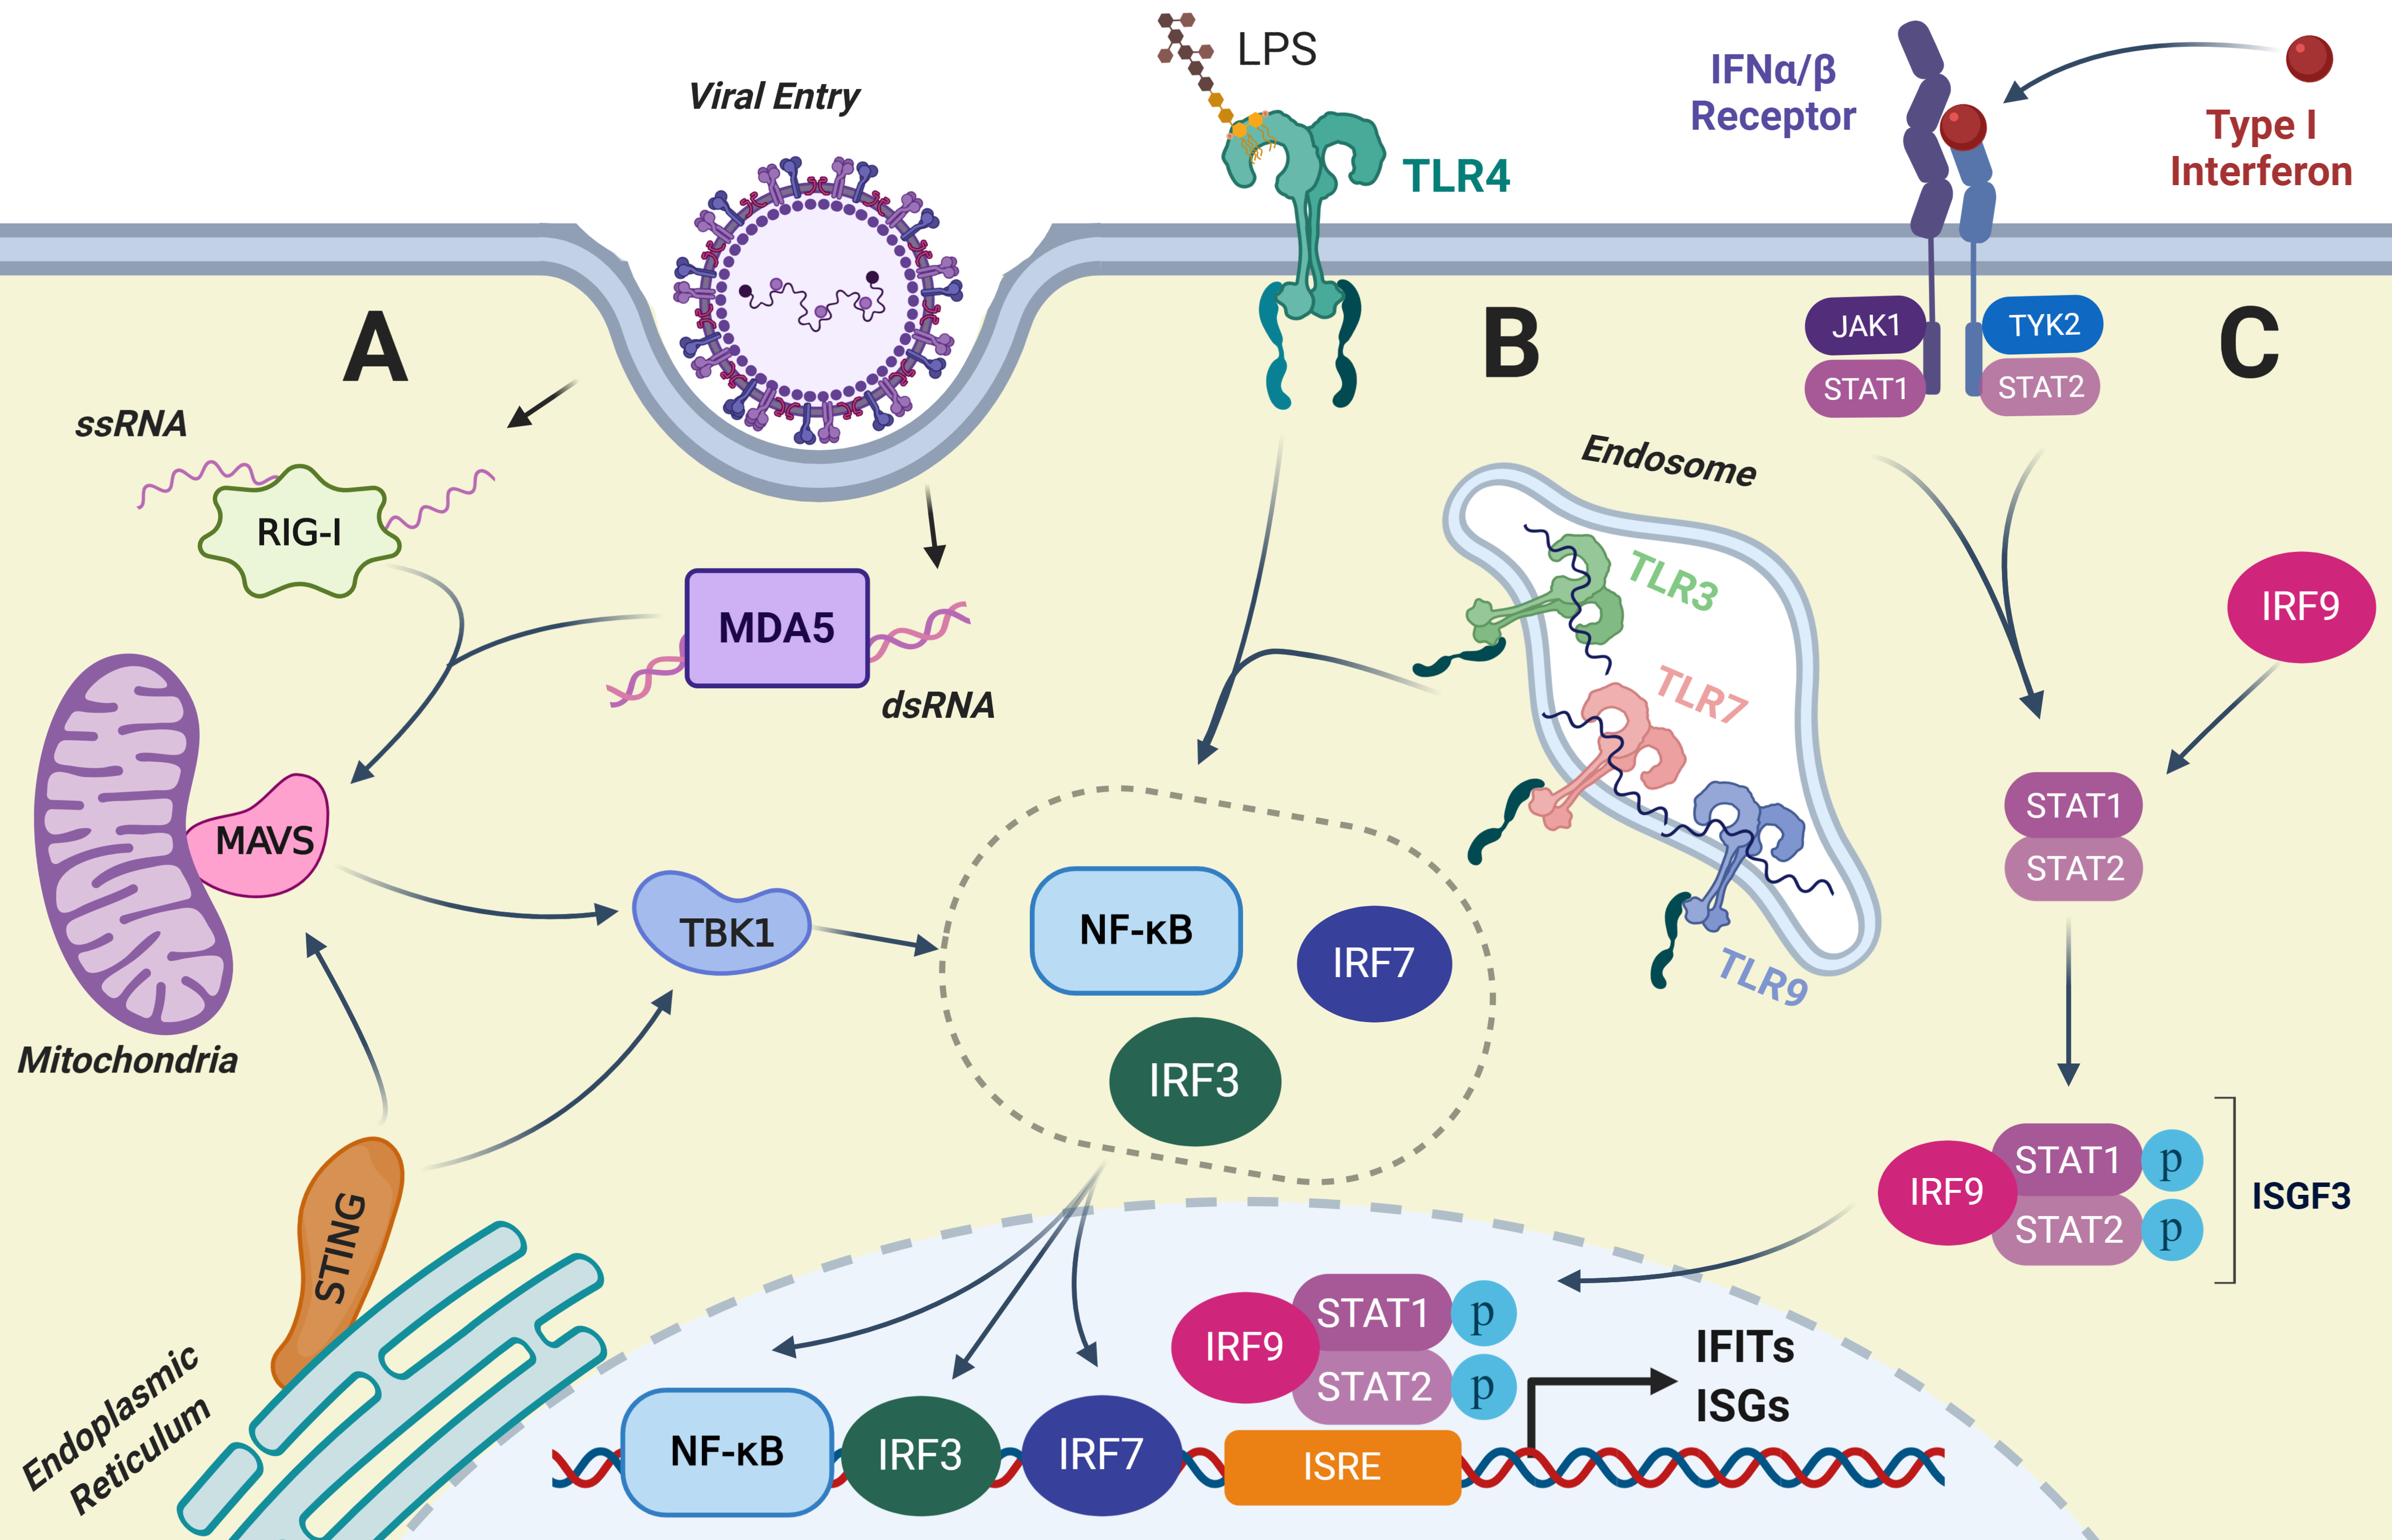
\includegraphics[width=1\linewidth]{04. Introduction//Figs/01. IFIT transcription activation figure.png}
    \caption[Pathways Inducing ISG mRNA Production.]{\textbf{Pathways Inducing ISG mRNA Production.} Three routes of ISGs transcription induction are depicted. Pathway A shows virus releasing its genome upon its entry and subsequent foreign nucleic acid detection by cytosolic sensors RIG-I and MDA5. These detect single-stranded and double-stranded RNA respectively. Both activate MAVS, which in turn activates TBK1. STING protein facilitates this activation by enhancing MAVS and TBK1 interaction. Pathway B shows PAMP detection by TLR receptors. TLR4 recognises LPS in the extracellular space while TLR3, TLR7, and TLR9 detect foreign nucleic acids in endosomes. TBK1, as well as TLR activation, leads to the translocation of activated IRF3, IRF7, and NF\(\kappa\)B into the nucleus where they promote ISGs transcription activation. Pathway C depicts type 1 interferon signalling pathway. IFN\(\alpha\)/\(\beta\) receptor activation leads to STAT1 and STAT2 activation. Further addition of IRF9 forms ISGF3 complex, which translocates into the nucleus onto ISRE and promotes ISGs transcription activation. ISG, interferon-stimulated genes; RIG-I, retinoic acid-inducible gene-I; MDA5, melanoma differentiation-associated gene 5; MAVS, mitochondrial antiviral signalling protein; TBK1, TANK-binding kinase 1; STING, stimulator of interferon genes; PAMP, pathogen-associated molecular pattern; TLR, toll-like receptor; IRF, interferon regulatory factor; NF\(\kappa\)B, nuclear factor kappa B; IFN, interferon; STAT, signal transducer and activator of transcription; ssRNA, single-stranded RNA; dsRNA, double-stranded RNA; ISGF, interferon-stimulated gene factor; ISRE, interferon-stimulated response elements. The figure was adapted from Diamond and Farzan, (2013) and Natalya Odoardi's BioRender template. Created with BioRender.com.}
    \label{fig:Pathways Inducing ISG mRNA Production.}
\end{figure}

\subsubsection{Cytosolic Nuclec Acid Sensors} \label{Cytosolic Nuclec Acid Sensors}
Cytosolic RNA sensors include melanoma differentiation-associated gene 5 (MDA5) and retinoic acid-inducible gene I (RIG-I) (\cite{Vladimer2014IFITs:Proteins}). Both signal through mitochondrial antiviral signalling protein (MAVS), which in turn activates IRF3, IRF7, and NF\(\kappa\)B as their downstream effectors (\cite{Ashley2019Interferon-IndependentCytomegalovirus}). In order to prevent activation by cellular RNA molecules, a precise RNA-recognition mechanism has to be conducted by the sensors. While MDA5 senses long double-stranded RNA (dsRNA) (\cite{Brisse2019ComparativeMDA5.}), RIG-I is able to sense differences in the 5' RNA modifications (\cite{Schlee2016DiscriminatingSensing}). During mRNA maturation in higher eukaryotes, 7-methyl guanosine (m7G) is connected by a 5'- 5' triphosphate bridge, which is referred to as capping (\cite{Devarkar2016StructuralRIG-I}; \cite{Ramanathan2016MRNAApplications}). Several viruses carry uncapped, 5'-triphosphorylated (5'-PPP) or incompletely capped RNA (cap 0), whereas host animals possess cap-1 and cap-2 mRNA moieties (\cite{Choi2018ACaps}), which are all depicted in Figure \ref{fig:Overview of 5'RNA Modifications.}. \textit{IFITs} can be activated by several signal transduction pathways, each with its own inducers and kinetics. A cross-play of these pathways is what in turn orchestrates IFIT response during viral infection.

\begin{figure}
    \centering
    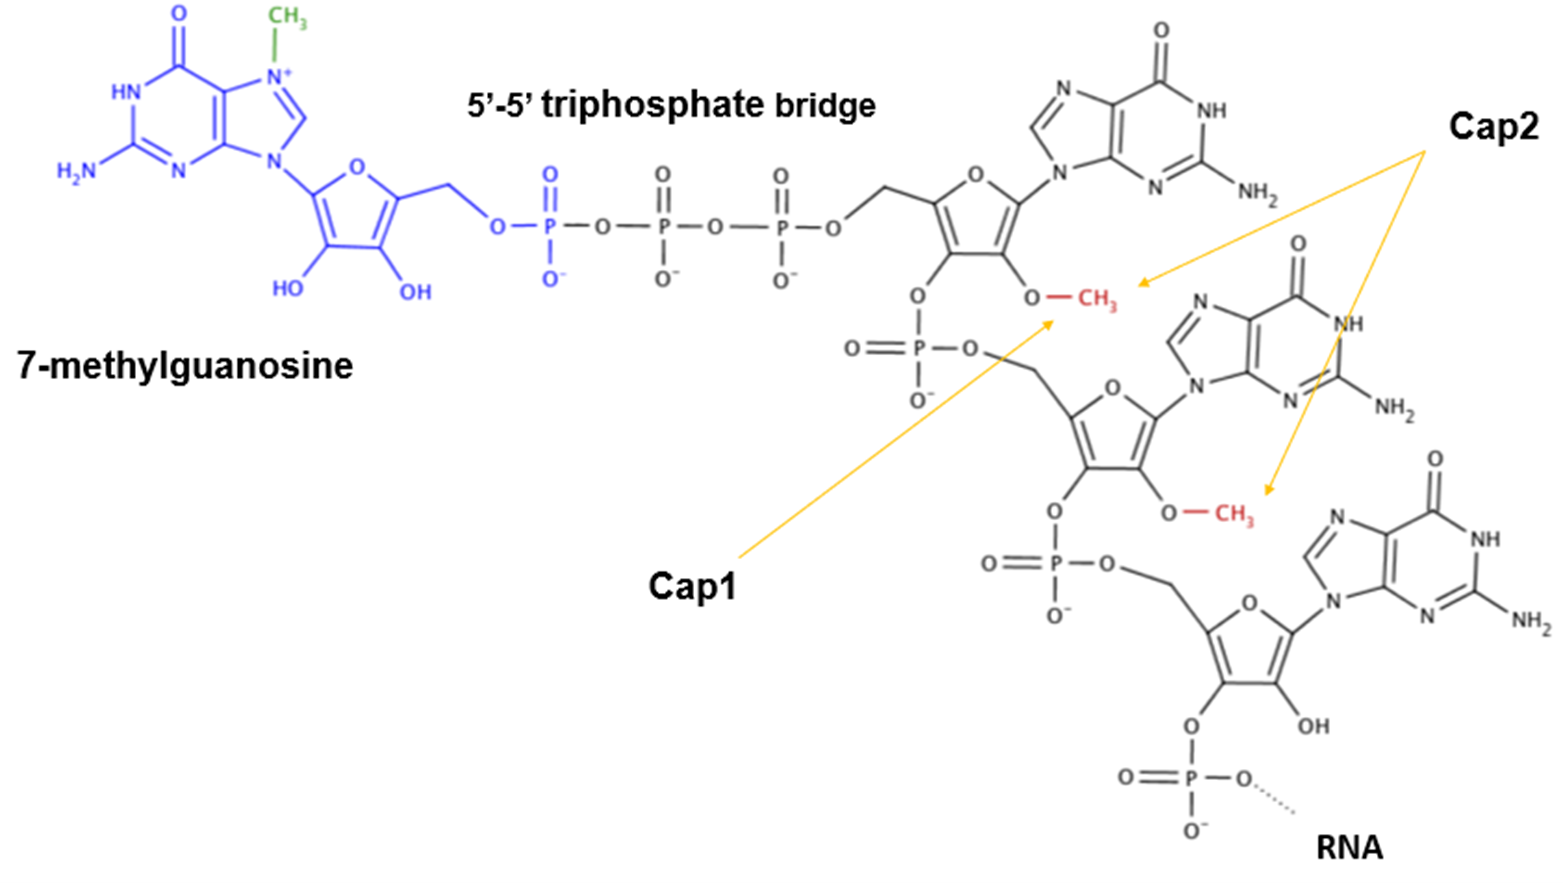
\includegraphics[width=0.75\linewidth]{04. Introduction//Figs/02. 5-RNA Modifications.png}
    \caption[Overview of 5'RNA Modifications.]{\textbf{Overview of 5'RNA Modifications.} Mature mRNA is displayed. Higher eukaryotes modify their mRNA by the initial addition of guanosine (blue) via 5' - 5' triphosphate bridge to the 5' end. Subsequently, the guanosine is methylated into 7-methylguanosine (green) and this modification is referred to as Cap0 structure. Furthermore, the first 2 bases of RNA can be methylated (red) and make either Cap1 or Cap2 structural modifications (yellow arrows). The figure was adapted from \cite{Picard-Jean2013RNAGenomes}.}
    \label{fig:Overview of 5'RNA Modifications.}
\end{figure}

\subsection{Structural Features of IFIT Proteins} \label{subsec:Structural Features of IFIT Proteins}
IFITs are composed of multiple copies of tetratricopeptide repeats (TPR). These are motifs comprised of 3-16 tandem repeats of 34 amino acids, which adopt helix-turn-helix confirmations (\cite{DAndrea2003TPRHelix}). TPRs are conserved in all species from bacteria through plants to higher animals and are commonly found in scaffolding proteins (\cite{Vladimer2014IFITs:Proteins}). IFIT TPRs are comprised of degenerate sequences meaning the conservation of the motif is limited. This allows different IFIT proteins to have a broader profile of protein interactors while still maintaining the overall conformation (\cite{Fensterl2015Interferon-InducedPathogenesis}). IFIT proteins are often subjected to post-translational modifications such as ubiquitination or ISGylation (addition of small IFN-induced ubiquitin-like proteins), which may alter IFIT stability and function.

\subsubsection{IFITs and Their Interaction with RNA} \label{IFITs and Their Interaction with RNA}
IFIT1 and IFIT5 both form a positively charged channel with an affinity for 5' ends of single-stranded RNA (ssRNA) molecules in a sequence non-specific manner. IFIT5 can accommodate 5'PPP RNA and effectively acts as a sensor for these molecules (\cite{Abbas2013StructuralProteins}; \cite{Pichlmair2011IFIT1RNA}). On the other hand, IFIT1 can accommodate m7G, but certain residues inside its channel prevent efficient binding of cap1 and cap2 moieties (\cite{Diamond2014IFIT1:Translation}; \cite{Mears2018BetterResponse}). Through these interactions they can effectively discriminate between self and non-self RNA moieties. IFIT2 is also capable of RNA binding, albeit independent on the 5'-capping state. The C terminals of IFIT2 homo-dimer create a super-helical structure with a positively-charged nucleotide-binding channel on its inner surface, which was observed to bind to AU-rich RNA molecules (\cite{Yang2012CrystalMechanisms}). Mechanistic studies identified IFIT2 binding to mRNAs as important to prevent ribosomal pausing and thus increasing the transnational efficiency of IFIT2-bound mRNAs, a process which has been observed to be hijacked by influenza A virus (\cite{Tran2020InfluenzaMRNAs}).

\subsubsection{Formation of IFIT Protein Complexes} \label{Formation of IFIT Protein Complexes}
As shown in Figure \ref{fig:IFIT Structures and Multimer Formation.}, all IFIT proteins, apart from IFIT5, can form homo- and hetero- dimeric and trimeric complexes. IFIT1 homodimerizes via its C-terminal domain (\cite{Abbas2013StructuralProteins}). The same domain has been shown to interact with the C termini of both IFIT2 and IFIT3, although the IFIT1:IFIT3 complex is more thermodynamically stable (\cite{Fleith2018IFIT3RNA}). Compared to IFIT1, IFIT5 has its dimerization motif shielded by its C terminal TPR and thus stays monomeric in solution (\cite{Kumar2014InhibitionMRNAs}). In contrast, IFIT2 and IFIT3 are rarely seen as monomeric in solution and rather stay as their respective homodimers or IFIT2:3 heterodimers. This is predicted to be done by swapping the third TRP domain in their N-terminal domains (Figure \ref{fig:IFIT Structures and Multimer Formation.}), which keeps them in a more thermodynamically stable configuration (\cite{Yang2012CrystalMechanisms}). IFIT2 homodimer forms a large positively charged cavity which has a propensity to bind dsRNA and AU-rich RNA molecules (\cite{Vladimer2014IFITs:Proteins}; \cite{Yang2012CrystalMechanisms}). IFIT3 interacts with IFIT1 via its C-terminal domain and this interaction increases the half-life of IFIT1 and its specificity for cap0 RNA. Thus, IFIT3 acts as an enhancer of IFIT1 action (\cite{Fleith2018IFIT3RNA}; \cite{Johnson2018HumanStability}). Recently, it has been shown that IFIT1, IFIT2, and IFIT3 form a heterotrimer, although the precise function of this complex has yet to be elucidated (\cite{Fleith2018IFIT3RNA}). In summary, TPR motifs allow IFITs to have a multitude of possible interaction partners, including themselves. Formation of IFIT homo- and hetero-oligomers influences their function and half-life, allowing for variable possible outcomes to occur following IFIT protein production based on the level of each of the proteins. 

\begin{figure}
    \centering
    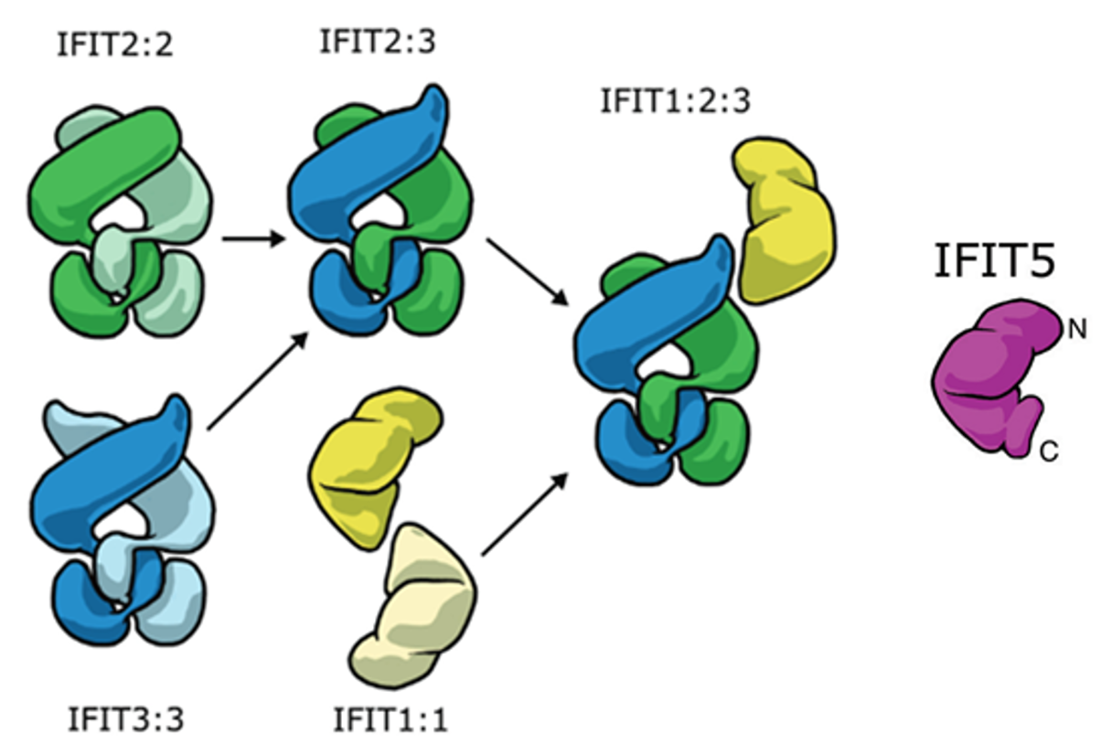
\includegraphics[width=0.75\linewidth]{04. Introduction//Figs/05. IFIT-complexes.png}
    \caption[IFIT Structures and Multimer Formation.]{\textbf{IFIT Structures and Multimer Formation.} IFIT tertiary and quaternary protein conformations are illustrated. IFIT1 is shown in yellow, IFIT2 in green, IFIT3 in blue, and IFIT5 is highlighted in purple. IFIT1 is able to homodimerise or heterooligomerise with IFIT2 and IFIT3 via its C terminal domain. IFIT5 has the corresponding interaction domain occluded by a helix and thus does not interact with the rest of IFIT proteins. IFIT2 and IFIT3 are capable of forming homodimers or heterodimers by ‘swapping’ TPRs in their N terminal regions. By combining the interactions IFIT1:2:3 heterotrimer is formed. The figure was adapted from \cite{Mears2018BetterResponse}.}
    \label{fig:IFIT Structures and Multimer Formation.}
\end{figure}

\subsection{Localisation and Functions of IFIT Proteins} \label{subsec:Localisation and Functions of IFIT Proteins}
\subsubsection{Localisation of IFIT Proteins} \label{Localisation of IFIT Proteins}
As with everything, loads of data on human and mouse models

IFIT1

\cite{}

IFIT2



IFIT3



IFIT5




\cite{Thul2017AProteome} - human protein atlas subcellular

\subsubsection{Inhibition of Translation and Viral Replication} \label{Inhibition of Translation and Viral Replication}
IFITs can restrict viral replication by several mechanisms. IFIT1 and IFIT5 can physically prevent non-self RNA from interacting with eukaryotic initiation factor (eIF) 4F (\cite{Kumar2014InhibitionMRNAs}). IFIT1 and 2 block the binding of eIF3 to the eIF2-GTP-Met-tRNA ternary complex by interacting with the eIF3E subunit, whereas human IFIT2, and mouse IFIT1 and IFIT2, can block the formation of the 43S-mRNA complex by binding to the eIF3C subunit (\cite{Diamond2014IFIT1:Translation}; \cite{Guo2000CharacterizationVirus}). This is a cap-independent mechanism for viral translation inhibition, however, extensive IFIT expression can negatively influence the whole cellular translation processes via this mechanism and can hinder normal inflammatory responses. Overexpression of IFIT1 in human embryonic kidney (HEK) 293T cells inhibited the activation of IRF3 and NF\(\kappa\)B and the transcription of IFN\(\beta\) in response to polyinosinic-polycytidylic acid (poly I:C) (\cite{Li2009ISG56Response}). The previously mentioned affinity of IFIT2 for AU-rich RNA can also regulate cellular translation as a lot of transcripts for cytokines or apoptotic factors are rich in adenine and uracil (\cite{Palanisamy2012ControlMicroRNAs}). 

\subsubsection{Modulation of Innate Immune Response Signalling} \label{Modulation of Innate Immune Response Signalling}
IFIT proteins also have the potential to influence innate immune responses by direct interaction with signalling cascade proteins. IFIT3 can potentiate RIG-I signalling by forming a scaffold between MAVS and TANK-binding kinase 1 (TBK1), (\cite{Liu2011IFN-InducedTBK1}), whereas IFIT5 enhances this pathway upstream by recruiting RIG-I to MAVS (\cite{Zhang2013IFIT5Pathways}). IFIT5 has also been reported to help facilitate NF\(\kappa\)B activation via scaffolding its activation kinases (\cite{Zhang2013IFIT5Pathways}). On the other hand, studies show that IFIT1 can both negatively and positively influence RIG-I signalling, upstream of MAVS. IFIT1 interacts with the stimulator of interferon genes (STING), an enhancer of MAVS and TBK1 interaction and it was proposed that these conflicting actions are caused by its multiple binding sites on STING (\cite{Li2009ISG56Response}; \cite{Reynaud2015IFIT1Interferon}). 

\subsubsection{Effects on Cell Cycle Progression and Apoptosis} \label{Effects on Cell Cycle Progression and Apoptosis}
IFIT2 and IFIT3 also have roles in cellular homeostasis. IFIT2 overexpression induces the mitochondrial dependant apoptotic pathway. IFIT2 has been shown to localise on mitochondrial membranes and to directly interact with pro-apoptotic factors which lead to apoptosome formation and subsequent caspase-9 activation (\cite{Chen2017InhibitionApoptosis}; \cite{Diamond2013TheProteins}). Expression of IFIT3 has been observed to alleviate these effects, most probably by the formation of IFIT2:3 dimers (\cite{Mears2018BetterResponse}; \cite{Stawowczyk2011TheApoptosis}). IFIT3 has also been observed to have negative effects on proliferation via indirect degradation of cyclin-dependant kinase inhibitor p27. As a result, cell cycle progression halts at the G1/S transition checkpoint (\cite{Xiao2006RIG-GProteins}). An overview of the IFIT mechanisms of action is depicted in Figure \ref{fig:Overview of IFIT Mechanisms of Action}.

Therefore, IFITs not only act as complementary RNA sensors to RIG-I but are also important as mediators of a plethora of other processes. These range from regulation of transcription, activation and inhibition of innate immune signalling, and regulation of cell life cycle. It is again possible that preference for these actions is influenced by the levels of particular IFIT proteins and their interplay. Taking into consideration the above-described modes of IFIT expression activation, we can speculate that different stimuli such as viruses or signalling molecules at different concentrations will result in quite diverging actions of IFIT proteins on the phenotype of the cell.

\begin{figure}
    \centering
    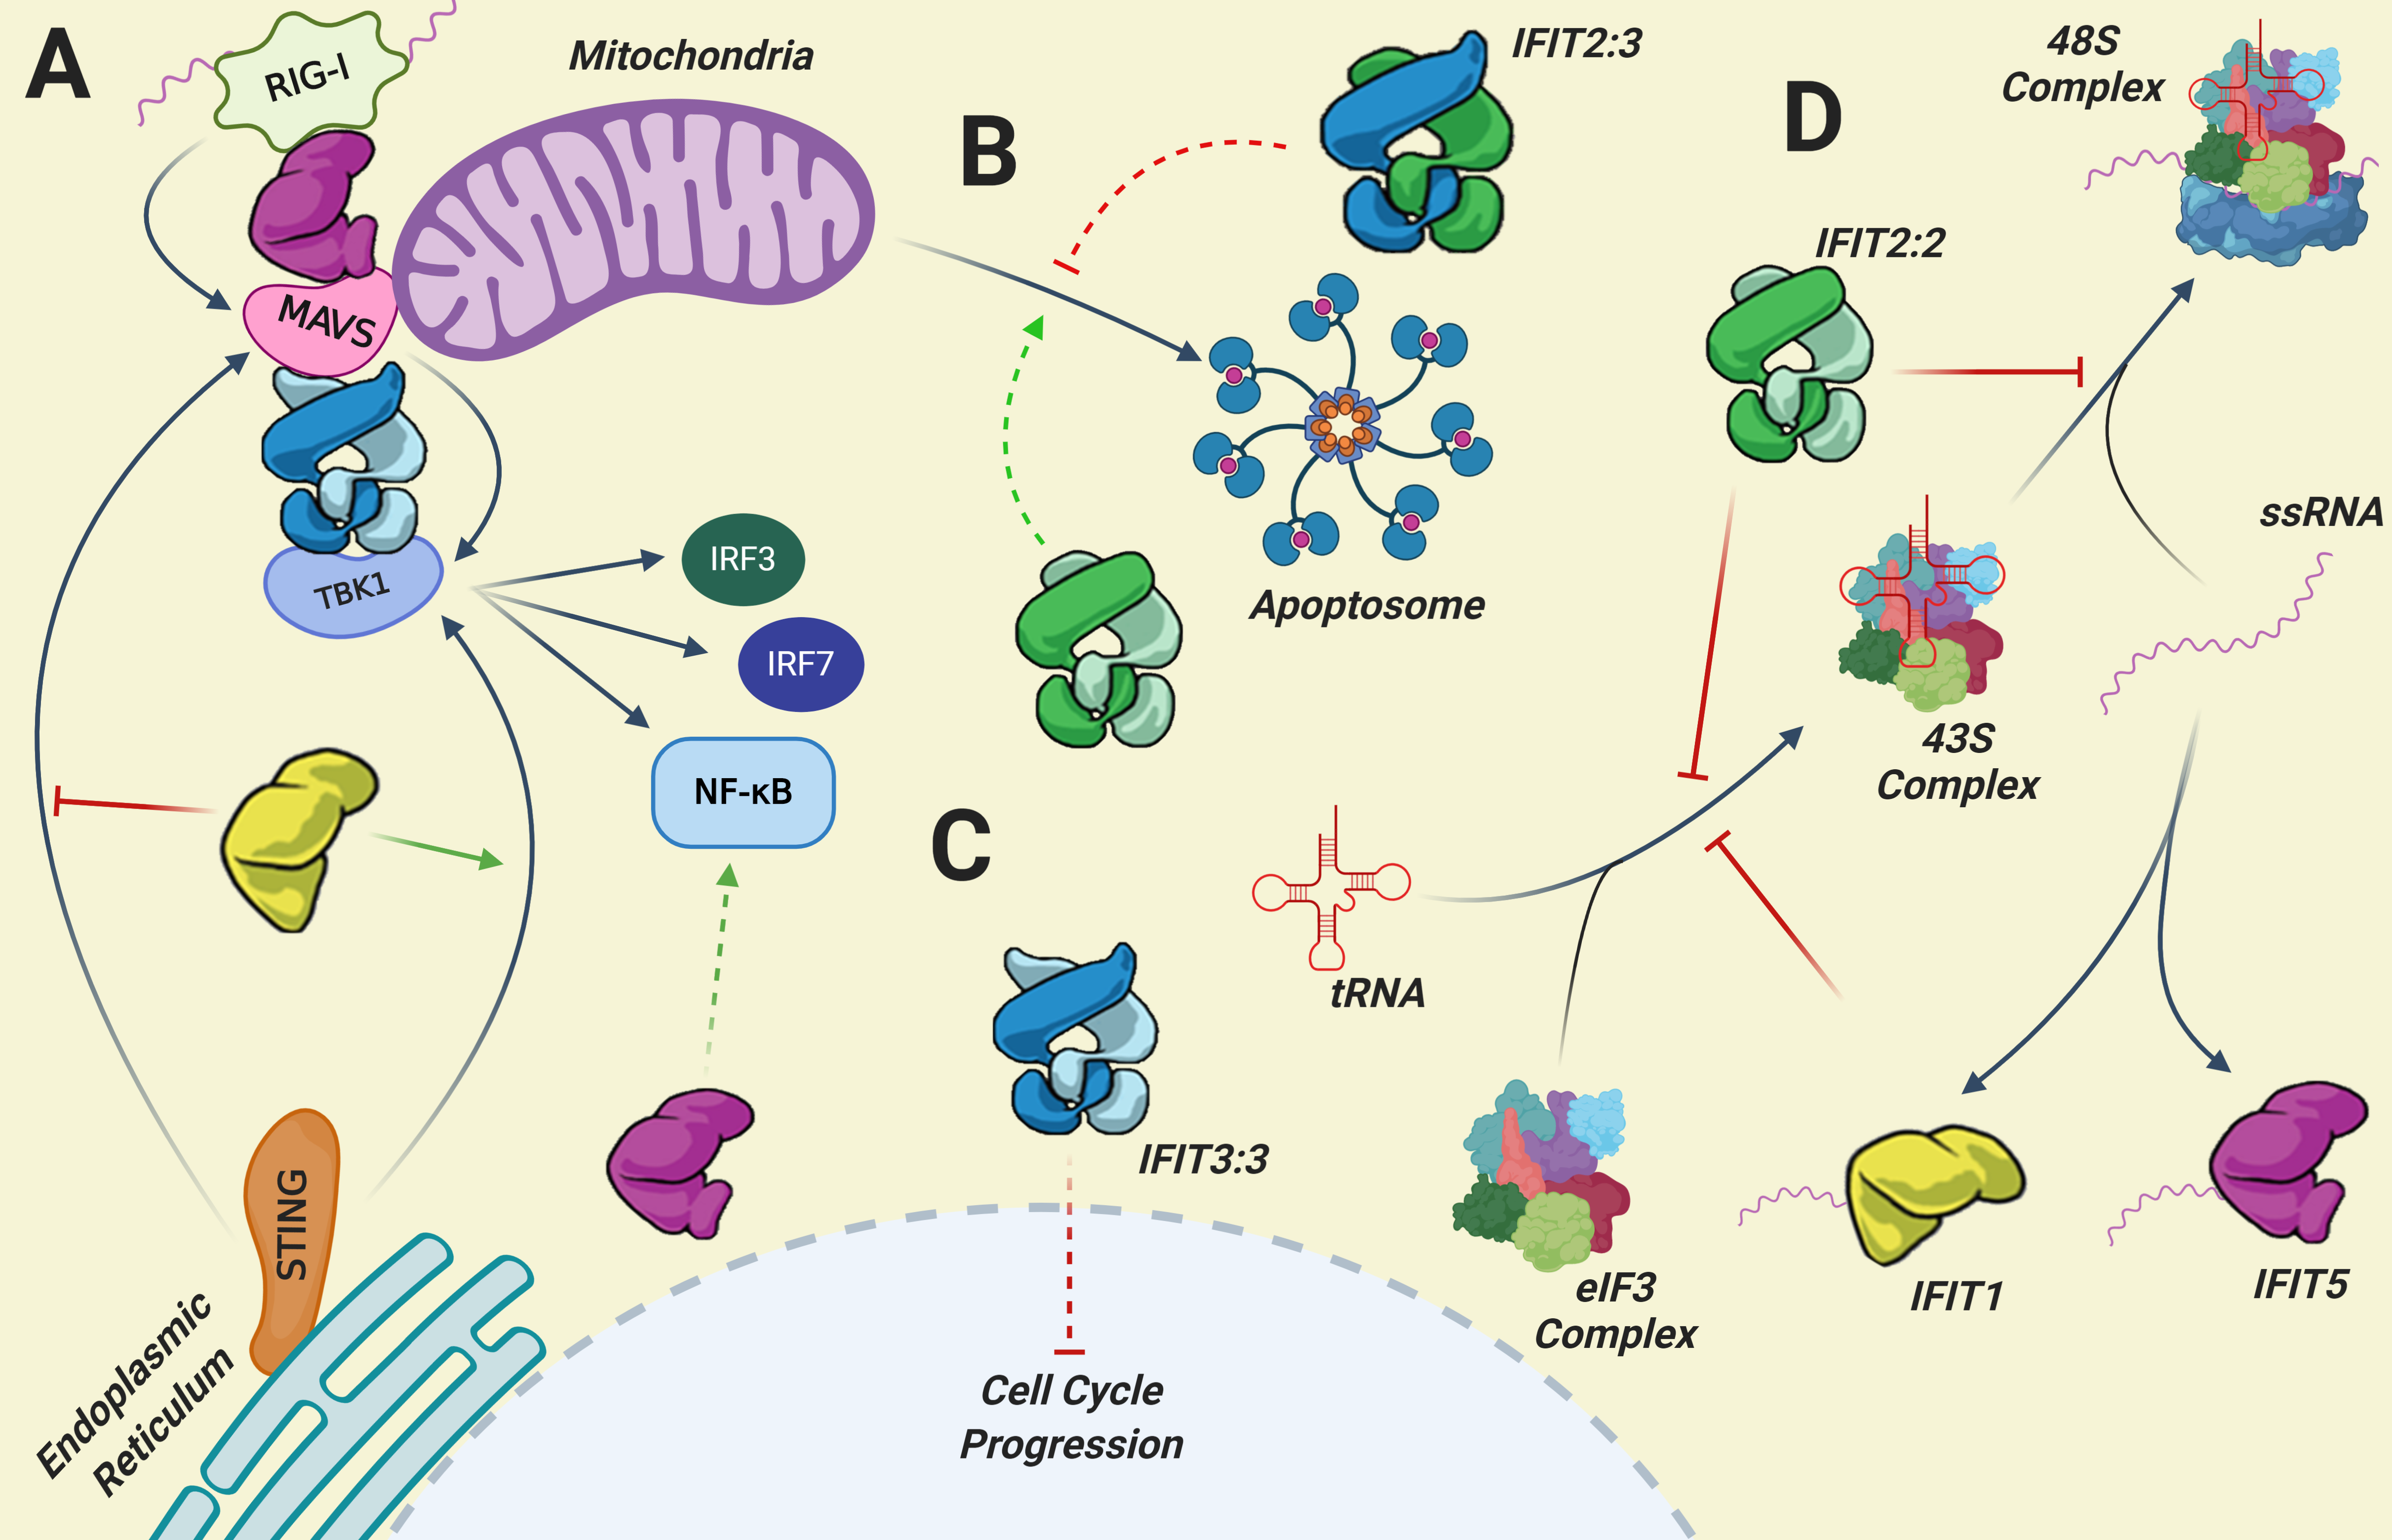
\includegraphics[width=1\linewidth]{04. Introduction//Figs/06. IFIT Mechanism of Action.png}
    \caption[Overview of IFIT Mechanisms of Action.]{\textbf{Overview of IFIT Mechanisms of Action.} IFITs have been described to have multiple actions in cells. Pathway A shows their involvement in innate immune signalling modulation. IFIT5 potentiate RIG-I activation of MAVS by scaffolding the two proteins together. IFIT3:3 further scaffolds MAVS to its effector, TBK1, which induces IRF3, IRF7 and NF\(\kappa\)B nuclear translocation when activated. STING protein also potentiates MAVS and TBK1 interaction. IFIT1 has been observed to inhibit STING interaction with MAVS while potentiating its interaction with TBK1. IFIT5 can also indirectly activate NF\(\kappa\)B. Pathway B shows IFIT2:2 involvement with apoptosome formation. IFIT2:3 complex reduces the pro-apoptotic activity of IFIT2:2. IFIT3:3 is involved in cell cycle arrest, as depicted in pathway C. Pathway D shows IFIT inhibition of viral replication and cellular translation. IFIT1 and IFIT5 can directly bind to cap0 and 5’PPP mRNA respectively and prevent its translation. IFIT1 and IFIT2 can both prevent 43S complex formation, while IFIT2 can also inhibit 48S complex formation. IFIT, Interferon-Induced Protein with Tetratricopeptide Repeats; RIG-I, retinoic acid-inducible gene I; MAVS, mitochondrial antiviral signalling protein; TBK1, TANK-binding kinase 1; STING, stimulator of interferon genes; IRF, interferon regulatory factor; NF\(\kappa\)B, nuclear factor kappa B; eIF, eukaryotic elongation factor; ssRNA, single-stranded RNA; tRNA, transfer RNA. The figure was adapted from \cite{Mears2018BetterResponse} and \cite{Diamond2013TheProteins}. Created using BioRender.com.}
    \label{fig:Overview of IFIT Mechanisms of Action}
\end{figure}

\subsection{IFIT Responses to Viral Infections} \label{subsec:IFIT Responses to Viral Infections}
Human IFIT effects on single-stranded RNA viruses have been studied extensively within the past decade. \cite{Rabbani2016Identification3} reported that IFIT1 and IFIT3 restrict human parainfluenza virus 3 (PIV3, negative-sense ssRNA virus), while ectopic expression of IFIT2 and IFIT5 did not affect the viral fitness. \textit{In vitro} IFIT1 knock-down experiments using short hairpin RNA showed marked enhancement of protein expression of human PIV2, PIV5, and mumps virus, all negative-sense ssRNA viruses (\cite{Andrejeva2013ISG56/IFIT1Synthesis}; \cite{Young2016HumanFamily}). Hantaviruses, a family of negative-sense ssRNA viruses such as Prospect Hill virus (PHV), and Tula virus (TULV), strongly induce IFIT3 expression during the course of their infection (\cite{Matthys2011TheInduction}). Most importantly within the non-segmented negative-sense ssRNA viruses, IFIT1, IFIT2, and IFIT3 have been reported to be globally antiviral against respiratory syncytial virus (RSV). Dori and colleagues either overexpressed or silenced these 3 IFITs and assessed RSV fitness by quantifying the viral mRNA produced. They reported decreased viral fitness following overexpression, while silencing of IFITs increased the viral mRNA production (\cite{Drori2020InfluenzaProteins}). Another negative-sense ssRNA virus, which bears a segmented genome, influenza A virus, has been shown to upregulate IFIT1, IFIT2, and IFIT3 in primary macrophages during infection (\cite{Lietzen2011QuantitativeMacrophages}). Recent studies also show the ability of IFIT1 and IFIT2 to negatively influence the viral fitness of influenza, as the knock-down of these IFITs resulted in increased viral RNA and protein production, while the opposite was true if IFIT1 and IFIT2 were overexpressed (\cite{Zhu2023TheSynthesis}). Human IFIT1 has been observed to be differentially expressed during hepatitis C virus (HCV) infection. HCV was described to suppress IFIT1 upregulation and subsequent experiments showed an inverse relationship between artificial levels of IFIT1 and HCV ability to infect host cells (\cite{Raychoudhuri2011ISG56Replication}, \cite{Ishida2019HepaticInfection}). Currently, there is very limited information about the effect of bovine IFIT expression on the viral fitness of bovine viruses.


\section{Respiratory Syncytial Virus} \label{sec:Respiratory Syncytial Virus}
Human and bovine Respiratory Syncytial Virus (hRSV and bRSV) are enveloped, negative-sense, single-stranded RNA viruses belonging to the Orthopneumovirus genus (\cite{Afonso2016Taxonomy2016.}). These viruses are recognized for inducing acute respiratory disease, which is confined to their respective hosts. Despite this host specificity, shared genetic and antigenic characteristics are observed among these closely related viruses (\cite{Buchholz2000ChimericVaccine}). hRSV primarily infects humans, while bRSV infects cattle. They are known to be the leading causes of lower respiratory tract illness in their respective hosts (\cite{Nair2013GlobalAnalysis.}; \cite{Sacco2014RespiratoryCattle}). Although these viruses can infect individuals of all ages, severe respiratory illness, including bronchiolitis and pneumonia, is more common in infants, the elderly, and immunocompromised individuals (\cite{AR2005RespiratoryAdults}; \cite{Coultas2019RespiratoryAge}). On a global scale, hRSV affects nearly all children by the age of five, resulting in approximately 33 million cases and 3.2 million hospital admissions annually (\cite{Shi2017GlobalStudy}). Tragically, around 60,000 hospitalized children under the age of five succumb to the infection, with a notably higher mortality rate among infants under six months, especially those at high risk due to factors such as premature birth and pre-existing chronic lung and heart conditions (\cite{Shi2017GlobalStudy}; \cite{Jha2016RespiratoryVirus}; \cite{Coultas2019RespiratoryAge}). Bovine RSV infection also poses a significant threat to the global cattle farming industry, resulting in substantial economic losses (\cite{Brodersen2010BovineVirus}; \cite{Valarcher2007BovineInfection}).

Despite extensive research and development efforts spanning several decades, the availability of approved vaccines against hRSV remains limited. Historical challenges include the failure of the formalin-inactivated RSV vaccine, which led to enhanced natural infection in some vaccinated children (\cite{Fulginiti1969RespiratoryVaccine}; \cite{Kim1969RespiratoryVaccine}). Additional hurdles involve the heterogeneity of RSV subtypes and the incomplete immune responses generated against the virus. However, recent advances in the field have introduced a range of vaccine strategies, including live-attenuated wild-type virus, vector-based, viral protein sub-unit, mRNA-based, and DNA-based candidates. Presently, 24 vaccines are in various stages of clinical development, including two licensed vaccines: Arexvy (GSK) and Abrysvo (Pfizer). These vaccines are used as immunizing agents to prevent lower respiratory tract disease in older adults, with Abrysvo additionally indicated for passive immunization of infants through maternal administration during pregnancy (\cite{Topalidou2023RespiratoryVaccines}). In contrast, there are several vaccines available for bRSV, with the first one dating back to the 1970s. However, these vaccines offer only mild protection. Consequently, there is a pressing need to develop more efficacious vaccines for both hRSV and bRSV (\cite{Ellis2017HowCattle}).

% from FJ
%%%%%%%%%%%%%%%%%%%%%%%%%%%%%%%%%%%%%%%%%%%%%%%%%%%%%%%%%%%%%%%%%%%%%%%%%%%%%%%%%%%%%%%%%%%%%%%%%%%%%%%%%%%%%%%%%%%%%%%%%%%%%%%%%%%%%%%%%%%%%%%%%%%%%%%%%%%%%%%%%%%%%%%%%
\subsection{Genomic and Virion Composition} \label{subsec:Genomic and Virion Composition}
Orthopneumoviruses have a linear negative-sense RNA genome, (15,223 nucleotides [nt] in length for hRSV A2 [GenBank accession no. KT992094] and 15,140 nt for bRSV A51908 [GenBank accession no. NC038272] which encodes genes for 11 proteins from 10 mRNAs. These are, in order from the 3' end: NS1, NS2, N, P, M, SH, G, F, M2, and L (Fig 1.1); and are flanked by 3' leader and 5' trailer sequences. This follows the typical genome organisation of mononegaviruses, encoding genes for a nucleoprotein (N), polymerase cofactor (P), matrix protein (M), surface glycoprotein (G) and polymerase (L) (Pfaller et al., 2015). M21 is The only exception is the M2 gene which has two slightly overlapping open reading frames (ORFs). 

Orthopneumoviruses may be distinguished from related viruses by the presence of four extra genes: NS1, NS2, SH and M2. Three of the encoded proteins (non-structural proteins; NS1 and NS2 and small hydrophobic; SH protein) are non-essential for virus replication but function in inhibiting innate immune signalling (Schlender et al., 2000, Spann et al., 2004, Pollock et al., 2017, Taylor et al., 2014, Bitko et al., 2007, Atreya and Kulkarni, 1999). NS1 and NS2 are not found in any other virus in the Mononegavirales order and have been shown to antagonise apoptosis (Bitko et al., 2007) and interferon (IFN)-mediated host responses by targeting both type I and II IFN induction (Schlender et al., 2000, Spann et al., 2004, Spann et al., 2005) and signalling (Lo et al., 2005). The two proteins localise in the cytoplasm, can form homotetramers, and work synergistically or individually (Schlender et al., 2000, Swedan et al., 2009). Specifically, NS2 interacts with a cytoplasmic nucleic acid receptor (RIG-I) inhibiting its interaction with the mitochondrial antiviral-signalling protein (MAVS) (Ling et al., 2009). Similarly, NS1 can inhibit phosphorylation of interferon regulatory factor 3 (IRF-3) by interacting with MAVS (Boyapalle et al., 2012) or by decreasing the levels of IKKε, a key protein kinase that specifically phosphorylates IRF3 (Swedan et al., 2009). The proteins can also decrease levels of other components of the interferon signalling pathway. NS1, and to a lesser extent NS2, mediate a decrease in the levels of TRAF3 in a non-proteasomal mechanism (Swedan et al., 2009). Recently, the NS proteins have also been shown to be involved in formation of an “NS -degradasome” that promotes the degradation of components of IFN induction or signalling, such as, RIG-I and IRF-3 and -7, TBK1 and STAT2 (Goswami et al., 2013). Consequently, activation of the cytotoxic T lymphocyte component of the adaptive immune response is also suppressed (Kotelkin et al., 2006).

The M2 gene which encodes the M2-1 and M2-2 proteins with roles in the regulation of viral RNA synthesis, is unique to members of the Pneumoviridae family and the basis for their recent separation from paramyxoviruses (Rima et al., 2017). These are expressed from overlapping ORFs, with expression of the second ORF using a unique mechanism of translation of the mRNA (Ahmadian et al., 2000, Gould and Easton, 2007, Powell, 2010). M2-1 is essential for virus replication and mainly localises in inclusion bodies (IBs) formed in the cytoplasm of infected cells (Rincheval et al., 2017). The details of viral transcription are discussed later, but briefly, once initiated at the 3' extragenic leader sequence, viral mRNA transcripts are produced sequentially from the 3' end of the genome in a stop-restart mechanism directed by gs and ge sequences that flank each gene (Kuo et al., 1996b). M2-1 acts as a transcription factor that prevents the early termination of the transcription machinery at ge signals, thus enhancing the transcription of genes towards the 5' end of the genome (Collins et al., 1995, Collins et al., 1996, Fearns and Collins, 1999b). M2-1 forms tetramers that can exist in phosphorylated and non-phosphorylated forms (Lambert et al., 1988, Tran et al., 2009). Phosphorylation was found to be important for hMPV replication and pathogenesis (Cai et al., 2016). The phosphorylation status of RSV M2-1 has been suggested to determine its interacting partners, localisation (cytoplasmic or intra-IB) and subsequent function (Richard et al., 2018). Both forms can interact with the P protein. However, interaction of phosphorylated M2-1 in the cytoplasm with P bound to a phosphatase, PP1, facilitates its dephosphorylation and recruitment into IBs, where they regulate viral mRNA transcription (Richard et al., 2018). M2-1 then binds and concentrates with the newly synthesised mRNA, an interaction which displaces P (Blondot et al., 2012, Tran et al., 2009, Cuesta et al., 2000). Phosphorylation then releases M2-1 from the mRNA destined for translation and free M2-1 may then restart the cycle by interacting with P (Richard et al., 2018). Whether M2-1 plays a role in translation remains unclear but an interactomics study has identified that M2-1 interacts with several cellular proteins involved in mRNA metabolism and translation (Bouillier et al., 2019). Separately, a CCCH zinc-binding motif, that usually plays a role in RNA binding, is found in the conserved functionally essential N-terminus of both RSV (Hardy and Wertz, 2000, Tang et al., 2001, Zhou et al., 2003) and MPV M2-1 (Cai et al., 2015). The exact role of this motif, other than stabilisation of the tetrameric complex (Esperante et al., 2013), is presently unclear. M2-1 was also shown to play a role in M protein IB localisation and its interaction with the ribonucleoprotein complex (Li et al., 2008, Kiss et al., 2014). M2-2 is encoded by the second ORF of the M2 gene and unlike M2-1 is an accessory protein, not essential for virus growth. However, deletion of this ORF from hRSV A2 resulted in host range-specific partial attenuation of the virus (Jin et al., 2000a). Its absence also increased viral mRNA transcription and expression of the antigenic proteins (F and G) whilst genome and antigenome replication were reduced in comparison (Bermingham and Collins, 1999, Jin et al., 2000a). This suggests that accumulation of the M2-2 protein, perhaps in later stages of infection when significant viral proteins are expressed, directs RNA synthesis in favour of genome and anti-genome replication by downregulating transcription (Collins et al., 2013). Since both processes use the same machinery and RNA template, a balance is important for efficient virus replication. In effect, M2-2 acts as an RNA synthesis regulatory factor, although the exact mechanism of this switch is not clearly understood. Viruses lacking the expression of this protein are currently being investigated as live-attenuated vaccine candidates with promising results (McFarland et al., 2020, McFarland et al., 2018). Recently, hMPV M2-2 protein was found to inhibit innate immune signalling by targeting MAVS (Chen et al., 2016, Kitagawa et al., 2017, Ren et al., 2014, Ren et al., 2012). A similar role has not been reported for orthopneumovirus M2-2 proteins and there is no significant sequence identity between the pneumovirus M2-2 proteins (Collins et al., 2013). The final extra orthopneumovirus gene, SH, encodes one of three surface glycoproteins found in the virus lipid envelope (Fig 1.2). Unlike the unique NS and M2 proteins, SH orthologs are found in some members of the paramyxoviridae family and their role will be discussed in section 1.3. The other encoded proteins, non-glycosylated structural protein M, glycoproteins G and F involved in attachment and entry into host cells, and components of the RNA-dependent RNA polymerase complex (RdRp), N, P and L, will be discussed in the next two sections.

\begin{figure}
    \centering
    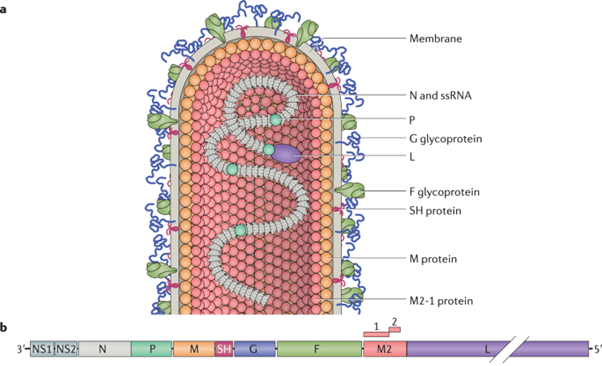
\includegraphics[width=1\linewidth]{04. Introduction//Figs/07. RSV-composition.png}
    \caption[RSV-composition]{\textbf{RSV-composition} }
    \label{fig:RSV-composition}
\end{figure}

\begin{figure}
    \centering
    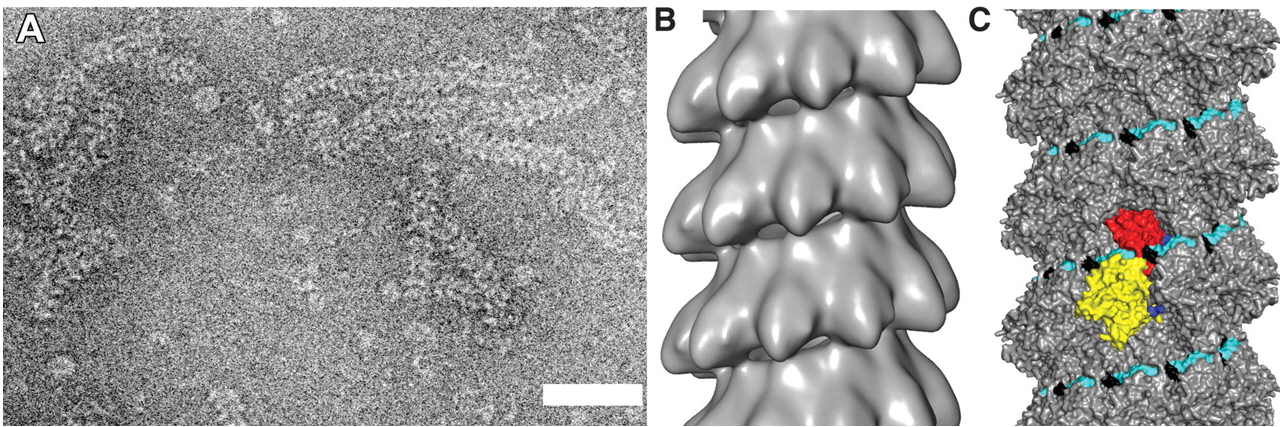
\includegraphics[width=1\linewidth]{04. Introduction//Figs/08. N-structure.jpeg}
    \caption[N-structure]{\textbf{N-structure} }
    \label{fig:N-structure}
\end{figure}

\begin{figure}
    \centering
    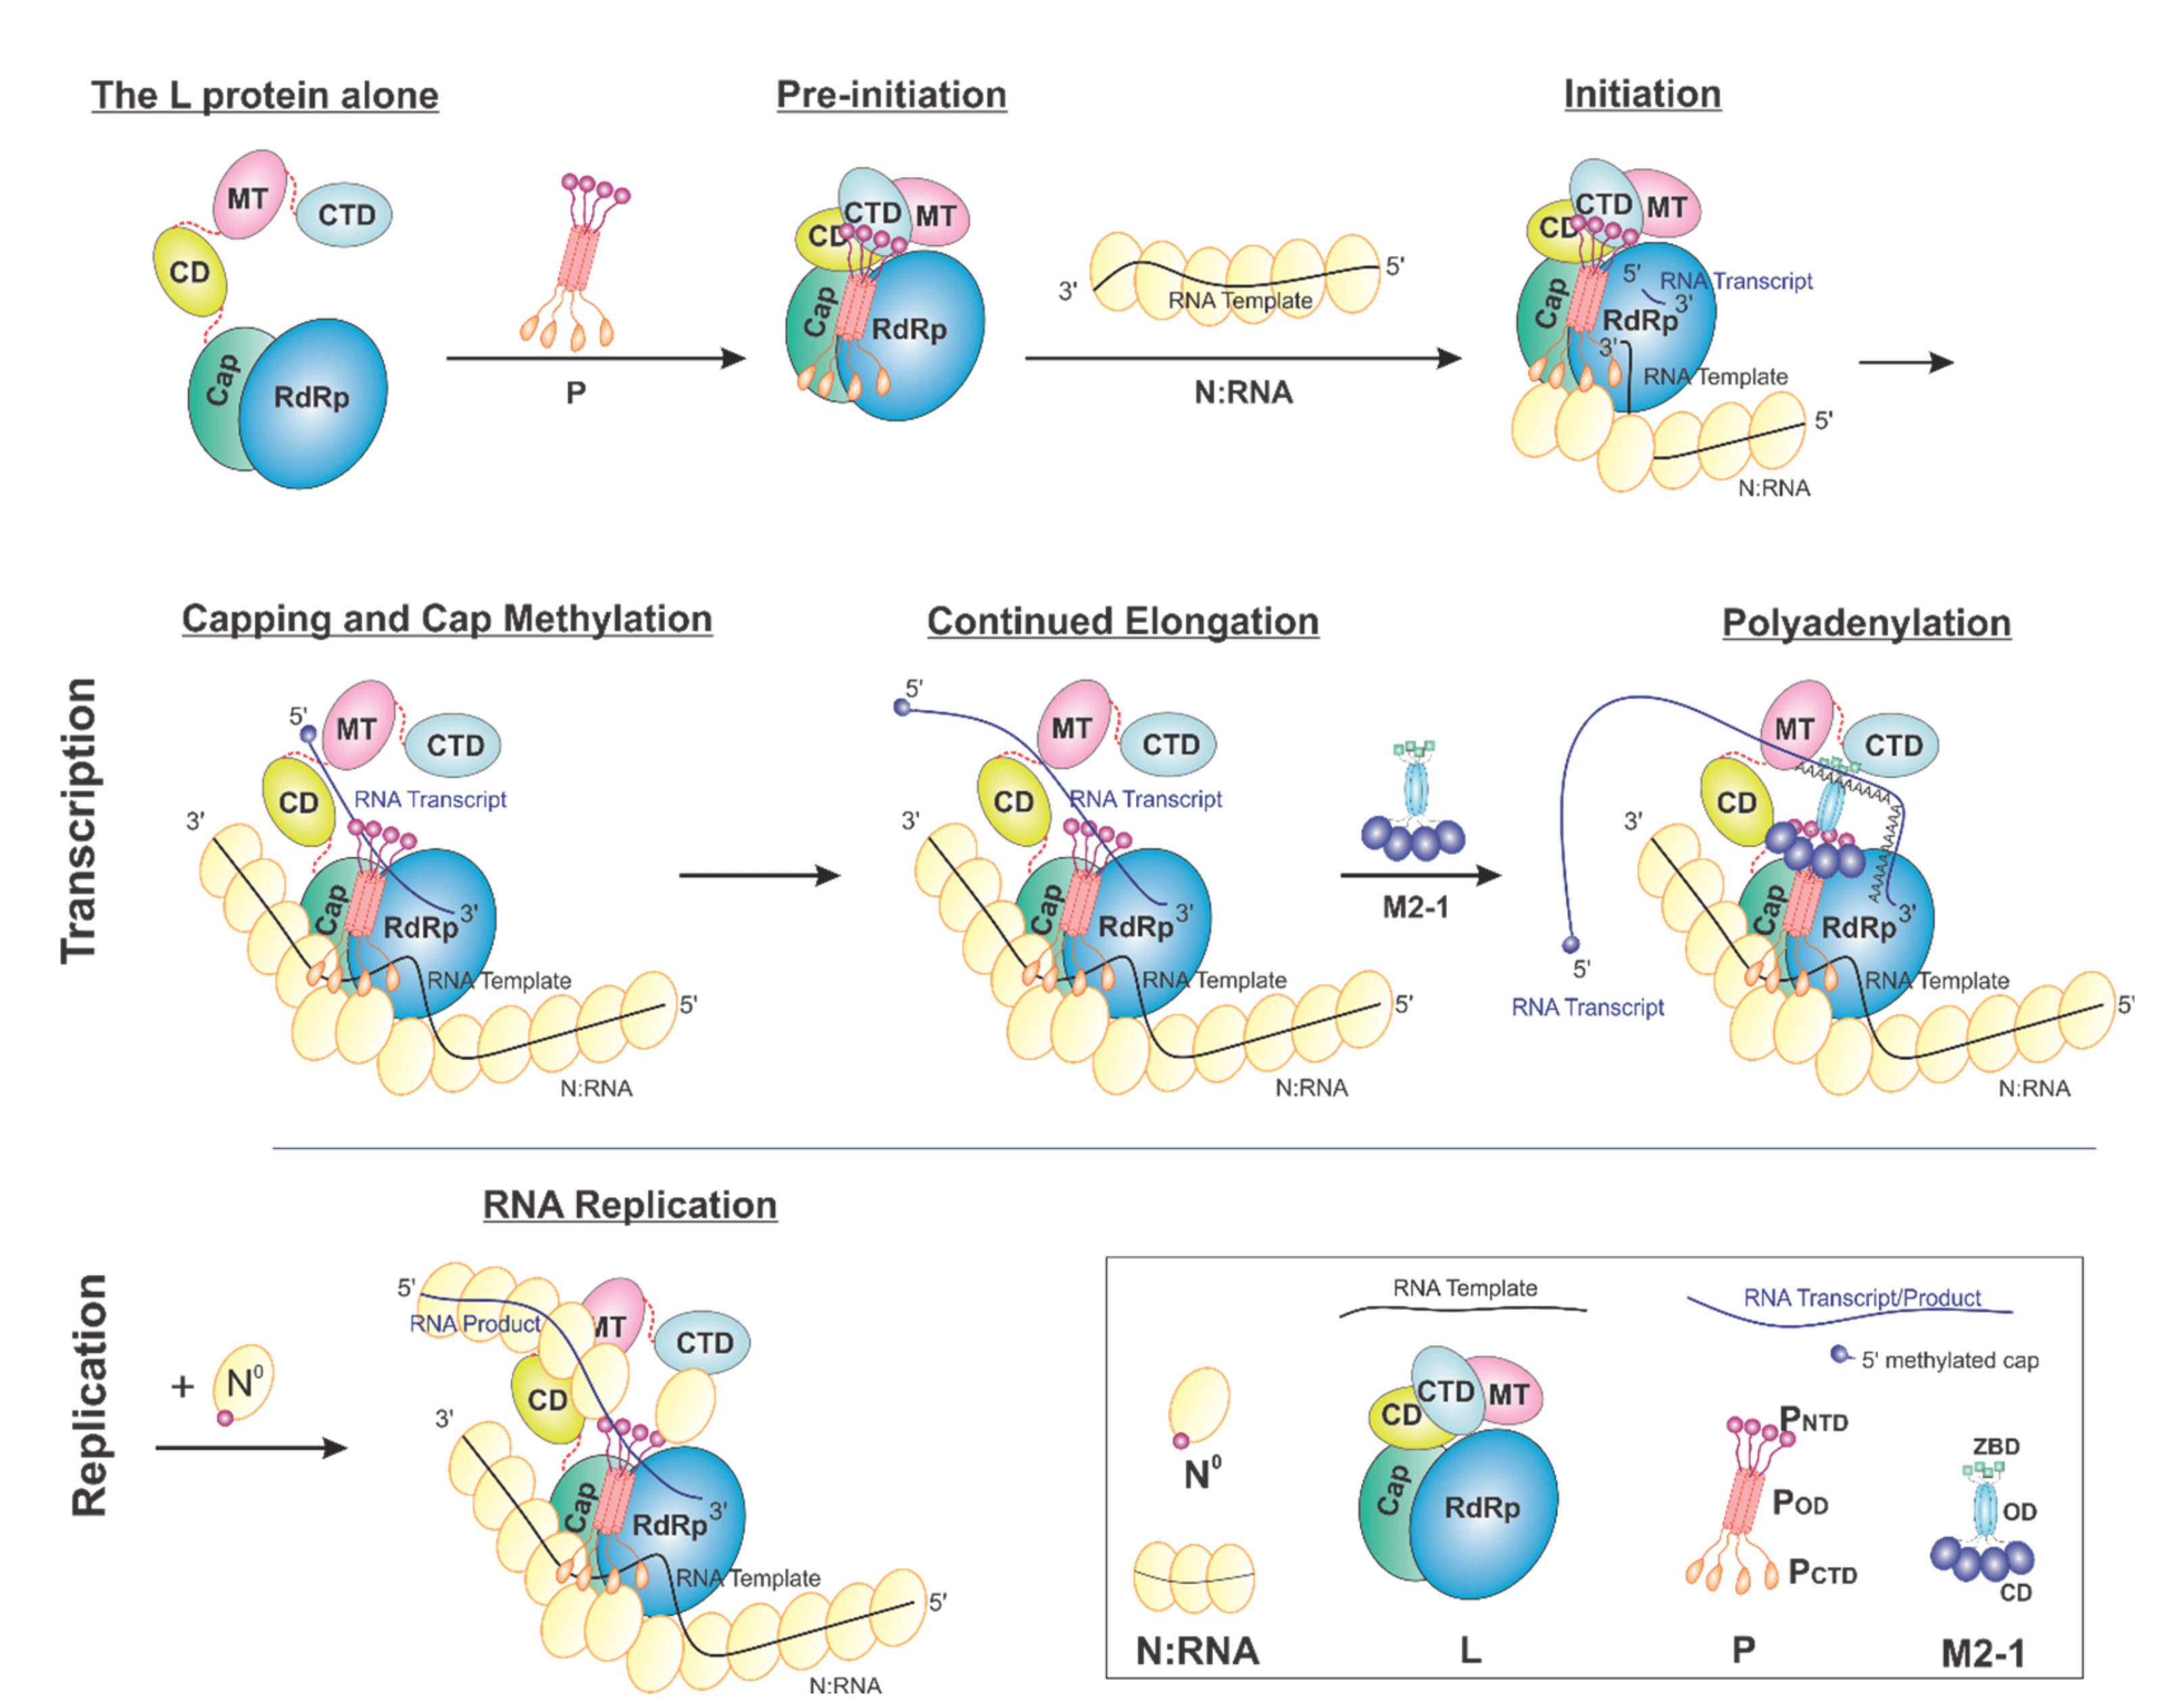
\includegraphics[width=1\linewidth]{04. Introduction//Figs/09. N_p_l_m21-interaction-overview.png}  
    \caption[Nplm21-interaction-overview]{\textbf{Nplm21-interaction-overview} }
    \label{fig:Nplm21-interaction-overview}
\end{figure}

Bovine and human RSV are enveloped viruses possessing negative-sense ssRNA genome approximately 15 kilobase-pairs in size. Upon viral attachment and entry, the genome is released into the cytoplasm in the form of a ribonucleoprotein i.e. a complex of RSV genome with its nucleoprotein (N protein) (\cite{Noton2015InitiationReplication}). Viral replication also requires the RNA-dependent RNA polymerase (L protein) and the phosphoprotein (P protein), whereas RSV transcription also requires M2-1 protein, which is hypothesised to prevent premature termination of this process (\cite{Tanner2014CrystalPhosphorylation}). RSV transcripts are modified with 5' cap structures prior to their translation. Both viral replication and transcription were previously believed to happen diffusely throughout the cytoplasm; however, recent studies suggest viral inclusion bodies (IBs) are the main site for RSV replication and transcription (\cite{Rincheval2017FunctionalVirus}). 

\subsection{Viral Life Cycle} \label{subsec:Viral Life Cycle}
put this quite simplified

\subsection{RSV Inclusion Bodies} \label{subsec:RSV Inclusion Bodies}
Human RSV infection is characterised by the formation of intracytoplasmic granules known as inclusion bodies (IBs; Fig 1.8) (Fricke et al., 2013, Lifland et al., 2012, Rincheval et al., 2017). These have been consistently observed both in vitro and in vivo (Norrby et al., 1970, Neilson and Yunis, 1990, Garcia et al., 1993, Lifland et al., 2012, Rincheval et al., 2017, Fricke et al., 2013), and are structurally and functionally similar to inclusions formed by several other viruses classified within the Mononegavirales order. This includes IBs induced by rabies virus infection termed Negri bodies (Lahaye et al., 2009, Nikolic et al., 2016, Nikolic et al., 2017), hMPV (Cifuentes-Munoz et al., 2017), MeV (Zhou et al., 2019), NiV (Ringel et al., 2019), and Ebola virus (Hoenen et al., 2012), and likely represent an essential component of the cellular cycle of many negative-sense RNA viruses. Recently, IBs were also observed in IAV infected cells, negative strand RNA viruses with a segmented genome (Alenquer et al., 2019). Interestingly, viral IBs also share many characteristics with biomolecular condensates called liquid organelles (Nevers et al., 2020). These form by liquid-liquid phase separation, LLPS, a process which favours macromolecular-macromolecular over macromolecular-water interactions (Banani et al., 2017, Uversky, 2017, Nevers et al., 2020, Alberti et al., 2019). The resulting structures have high molecular density, are composed of RNA and proteins (mostly RNA-binding proteins, RBPs), and also lack surrounding membranes, unlike classical organelles. These organelles are not exclusive to pathogens; cellular examples of biomolecular condensates include stress granules and P-bodies that form in the cytoplasm, and nucleoli and Cajal bodies found in the nucleus (Gomes and Shorter, 2019, Banani et al., 2017). They can be identified by their liquid-like properties based on the following criteria: spherical shape, ability to rapidly undergo fusion and fission, and their high fluidity/dynamic state when assessed by fluorescence recovery after photobleaching (FRAP) (Gomes and Shorter, 2019, McSwiggen et al., 2019, Alberti et al., 2019).



\subsubsection{Assembly of RSV IBs} \label{Assembly of RSV IBs}
With regards to viral IBs – biomolecular condensates formed in the context of virus infection – several have been shown to have liquid-like properties based on the criteria currently used for defining liquid organelles. These include cytoplasmic inclusions induced in RSV (Rincheval et al., 2017), MeV (Zhou et al., 2019), VSV (Heinrich et al., 2018), rabies (Nikolic et al., 2017) and ebola (Hoenen et al., 2012) virus infected cells, formed through the process of LLPS (Alberti et al., 2019, Nevers et al., 2020). However, the exact mechanism of their formation is less well characterised. RSV IBs appear in the cytoplasm at around 6h post infection, as viral proteins are expressed and grow in size as infection proceeds (Fricke et al., 2013, Lifland et al., 2012, Rincheval et al., 2017). Although they colocalise all proteins of the polymerase complex (Fig 1.8), for RSV, rabies and measles viruses, the N and P proteins are the minimum components essential for their formation in the absence of infection (Lifland et al., 2012, Nikolic et al., 2017, Rincheval et al., 2017, Zhou et al., 2019). Co-expression of the N and P proteins alone results in the formation of IB-like structures (pseudo-IBs) with similar properties to the viral inclusions. For VSV, the minimal system requires the presence of L (Heinrich et al., 2018). Viral IBs are essentially condensates of RNA and protein as proven by the large amounts of nucleocapsids and viral mRNA contained in these structures (Fig 1.9). The minimal system however does not rule out the involvement of RNA interactions in formation of the structures as cellular RNA may be used in the absence of virus infection. More recently, the N and P proteins of RSV (Galloux et al., 2020b) and MeV (Guseva et al., 2020) were shown to induce liquid droplets outside of the cellular environment, thus showing they are the main drivers of viral phase separation. However, there was a discrepancy between the two viruses in cells as the formation of pseudo-IBs by RSV N and P required N:RNA interaction (Galloux et al., 2020b); however, the MeV proteins did not (Guseva et al., 2020, Zhou et al., 2019). Guseva et al. further showed that although RNA is dispensable for MeV N:P phase separation, it preferentially colocalises to and triggers assembly of nucleocapsid-like particles within the structures formed.

Similar to cellular proteins involved in inducing LLPS, assembly of ectopically expressed N and P proteins into inclusions has been shown to involve oligomerisation and intrinsically disordered domains within these viral proteins (Zhou et al., 2019, Nikolic et al., 2017, Galloux et al., 2020a). The higher degree of intrinsic disorder within P proteins of RSV (Gilman et al., 2019, Pereira et al., 2017), MeV and rabies virus (Nevers et al., 2020, Longhi et al., 2017) suggests it has a greater propensity to phase separate but the involvement of N shows there are crucial mechanisms provided by this protein. Mechanistically, for RSV, the central oligomerisation domain and Cterminal domain (an intrinsically disordered region) of P, plus the ability of N to interact with both P and RNA, were shown to be required for pseudo-IB formation (Galloux et al., 2020b). Despite sequence variability, similar intrinsically disordered and oligomerisation domains are present in rabies and MeV P proteins (Nevers et al., 2020), and were also shown to be required for pseudo-IB formation (Nikolic et al., 2017, Zhou et al., 2019). Therefore, it appears that the N and P proteins and RNA (depending on the virus) are the “scaffolds” required for IB formation. Thus, as the concentrations of the viral proteins increase during infection, oligomerisation of P, multiple interactions facilitated by the intrinsically disordered regions of N and P (Pereira et al., 2017) and interactions with viral RNA (Galloux et al., 2015) could act in synergy to initiate phase separate and nucleation of the IB. These may then mature and grow in size as they further colocalise newly synthesised viral RNA and protein. Of note, several other viral protein-protein and protein-RNA interactions which could contribute towards maturation exist in IBs. For instance, the viral nucleocapsid which concentrates in IBs (Fig 1.8 and Fig 1.9), is composed of genomic RNA, N, L and P proteins (Fig 1.2) (Easton et al., 2004). M2-1 also can form multiple interactions - with P (Mason et al., 2003, Richard et al., 2018), M (Li et al., 2008) and viral mRNA (Rincheval et al., 2017). However, the process of maturation appears to be a complex and regulated process as indicated by the organisation of the condensates into multi-phasic structures. Rincheval et al. recently demonstrated the presence of sub-compartments within RSV IBs with distinct protein and RNA composition, biophysical properties and functions termed inclusion body associated granules; IBAGs (Rincheval et al., 2017). M2-1 and newly synthesised viral mRNA, presumably interacting, mainly localised to these IBAGs (Rincheval et al., 2017). This is similar to the distinct, coexisting liquid phases that make up the nucleolus (Feric et al., 2016). The IBAGs are dynamic structures, and their contents are subsequently released to the cytoplasm. However, further investigation is required to understand the mechanism underlying the evolution of biomolecular condensates from a single phase to sub-compartments carrying out distinct functions.

\begin{figure}
    \centering
    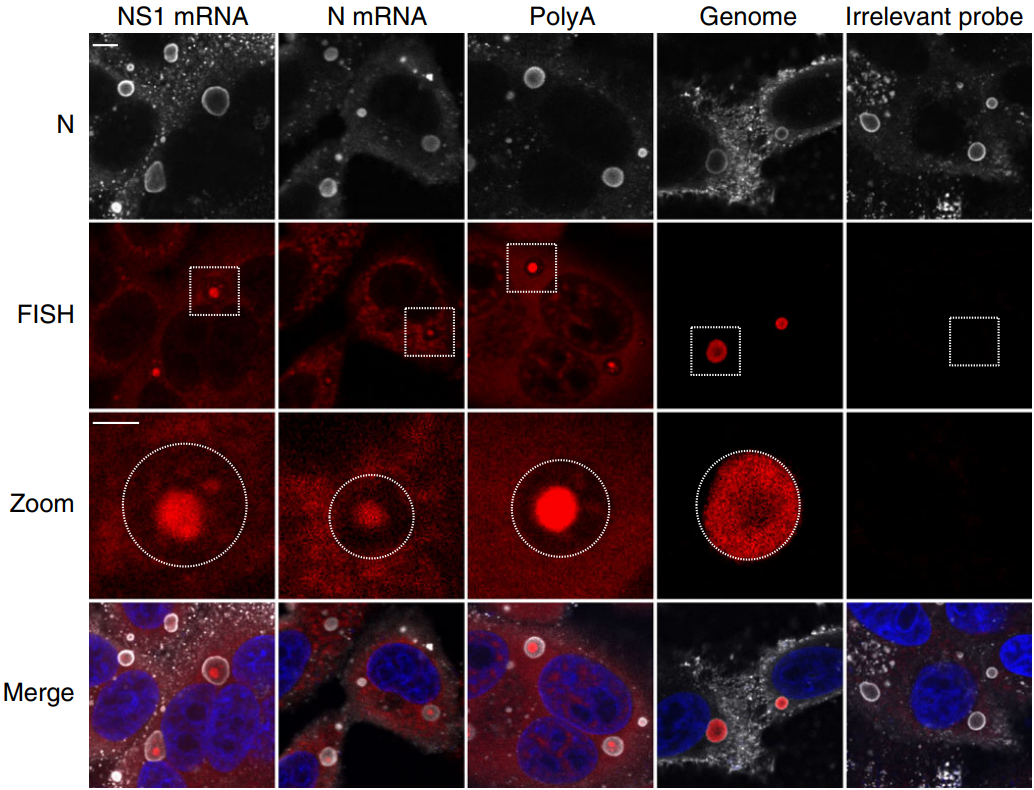
\includegraphics[width=1\linewidth]{04. Introduction/Figs/11. RSV IBs.png}  
    \caption[RSV IBs]{\textbf{RSV IBs} }
    \label{fig:RSV IBs}
\end{figure}

\subsubsection{Function of RSV IBs} \label{Function of RSV IBs}
The formation of membrane-less liquid organelles allows cells to spatially compartmentalise specific cellular processes whilst allowing biomolecule exchange with the cyto-/nucleoplasm (Banani et al., 2017, Gomes and Shorter, 2019). Viruses also appear to use biomolecular condensation for a multitude of virus-virus/virus-host interactions with the advantage of increasing the efficiency of replication. Prominent examples include IBs which are essentially replication complexes and sites of nucleocapsid assembly (Nevers et al., 2020), and also lipid rafts where particle assembly takes place (McDonald et al., 2004). The functional compartmentalisation of viral proteins and replication intermediates into inclusion bodies also minimises their interaction with factors of the host immune response. The exact role of IBs induced during infection was previously unclear and initially thought of as “aggregates of viral nucleocapsids” (Garcia et al., 1993). Recent evidence shows it is a common mechanism used by several mononegaviruses and further demonstrates their involvement in processes such as viral RNA replication and host immune modulation (Nevers et al., 2020).

Analysis of hRSV infected cells by immunofluorescence (IF) microscopy shows concentration of several viral proteins within IBs including N, P, L, M2-1, M and NS2 (Carromeu et al., 2007, Garcia et al., 1993, Lindquist et al., 2010, Brown et al., 2005, McDonald et al., 2004, Ghildyal et al., 2002). Most of these viral proteins are directly/indirectly associated with the nucleocapsid, explaining their colocalization within the structure. Interestingly, all of the proteins involved in transcription and replication (N, P, L and M2-1) co-localise in the IBs, whereas the surface glycoproteins are excluded. Recent identification of viral genomic RNA and mRNA within the IB (Fig 1.9) strongly suggests that these organelles are functional and are the primary site for viral RNA replication and transcription within the infected cell (Rincheval et al., 2017). Interestingly, distinct spatial organisations were observed between viral genomic and mRNA. As already noted above, mRNA concentrated in IBAGs whereas genomic RNA mostly localised towards the boundary of the IB (Fig 1.9). Further study is required to understand the significance of this organisation. Similarly, IBs produced in rabies (Lahaye et al., 2009) and ebola (Hoenen et al., 2012) virus infected cells were also shown as the sites of RNA replication and transcription. However, this does not appear to be universal a trend since viral RNA replication of Nipah virus (NiV) was recently shown to occur outside both its structurally distinct IB populations (Ringel et al., 2019).

As discussed in sub-section 1.2.3, a number of host cell proteins have been shown to interact with or co-localise within RSV induced IBs. These include antiviral proteins MAVS and MDA5 (Lifland et al., 2012), and signalling proteins involved in the cellular response to viral infection – p38 mitogen-activated protein kinase (MAPK) and O-linked N-acetylglucosamine transferase (OGT) (Fricke et al., 2013). In addition, the chaperone protein, HSP70 that protects cells from stress, has also been observed within RSV IBs (Brown et al., 2005). MDA5 and MAVS sequestration into IBs were shown to result in a reduction of IFNβ mRNA induction (Lifland et al., 2012). Similarly, sequestration of p38 MAPK and OGT suppressed MK2 activity and stress granule assembly. Recruitment of these key signalling proteins into IBs following RSV infection appears to be an additional mechanism of immune antagonism whereby their roles are inhibited through sequestration. However, whether these integrate with the scaffolds during the process of IB formation or associate with the granules as they mature, remains to be elucidated. Of note, viral IBs are induced in the early stages of infection, at a time when activation of innate immune signalling pathways is crucial. Thus, the use of IBs for innate immune antagonism is an important phenomenon for enhancing virus fitness during infection. Currently, it is unclear how broad this mechanism for regulating host antiviral responses is for viruses that induce cytoplasmic IBs. Much of what is currently known is on RSV IBs (Lifland et al., 2012, Fricke et al., 2013, Brown et al., 2005), although cellular WD repeat-containing protein 5 (Zhou et al., 2019, Ma et al., 2018), heat shock protein 72 (Zhang et al., 2005b) and actin-modulating protein cofilin (Koga et al., 2015) were also observed in measles virus IBs. Localisation of WD repeat-containing protein 5 in IBs was shown to enhance virus infection (Ma et al., 2018). It is therefore essential that further research is conducted to determine the scope of this strategy of immune modulation and to examine the implications for host responses to infection.
%%%%%%%%%%%%%%%%%%%%%%%%%%%%%%%%%%%%%%%%%%%%%%%%%%%%%%%%%%%%%%%%%%%%%%%%%%%%%%%%%%%%%%%%%%%%%%%%%%%%%%%%%%%%%%%%%%%%%%%%%%%%%%%%%%%%%%%%%%%%%%%%%%%%%%%%%%%%%%%%%%%%%%%%%

IBs are amorphous membranelles aggregates, which have been observed to form as early as 6 hours post-infection and often localise in close proximity to the nucleus (\cite{Bachi1973MorphogenesisVirus}; \cite{Jobe2020RespiratorySignaling}). They have characteristics of biomolecular condensates (with a similar electron density under electron microscopy to the nucleoli) and resemble cytoplasmic inclusions associated with other viral infections e.g. Negri bodies forming during rabies virus infection (\cite{Nikolic2017NegriOrganelles}). RSV N and P proteins are found on the edges of IBs, while L and M2-1 proteins are located inside the structure. (\cite{Rincheval2017FunctionalVirus}), using super-resolution imaging, discovered internal IB compartments called IB-associated granules (IBAGs). These not only contained different viral proteins compared to the rest of the IB, but nascent RNA labelling also suggested IBAGs to be the sites where newly synthesized mRNA concentrates (\cite{Jobe2020RespiratorySignaling}; \cite{Richard2018RSVTranscription}). Taken together, data suggests that IBs are specialised sites which enable viral replication and transcription and that these processes may be compartmentalised.

It is currently unknown if IFIT proteins interact with these structures. Given the well-described roles of IFITs in sensing viral RNA, it is possible that different IFITs may localise into IBs and IBAG, potentially interacting with viral RNA before the capping process takes place or directly interfere with the translational machinery. It is also possible that IFITs are restricted from accessing IBs by an unknown mechanism. Understanding these processes may reveal novel routes of increasing viral sensitivity to the innate immune response.



\section{Aims of the Study} \label{sec:Aims}
Here have a page of the aims.

A detailed comparative study of human and bovine IFITs and their interaction with RSV. Looking at their induction, expression, and changes in localisation. Looking at interaction with RSV IBs. Assessing the involvement of IFIT2 in the RSV life cycle.

For your Aims make sure these are very detailed, so 2 pages roughly. Not 3-4 bullet points of 2 lines each, which I have seen!

clearly human ifits are global restictors of hrsv. but is it relevant, do they get induced? can we isolate what is inducing them if so? 

are human ifits induced by brsv and thus have a potential to crossprotect from it?

does this reproduce in bifit with brsv and crossprotection from hrsv?

through what mechanism are ifits inhibitory? where are they located during infection?

do they interact with parts of rsv stuff?

is there a difference between ifits in interaction with htese structures?

%acronyms
\nomenclature[z-DEM]{DEM}{Untranslated}

\nomenclature[z-IBAG]{IBAG}{IB-Associated Granule}
\nomenclature[z-IB]{IB}{Inclusion Body}
\nomenclature[z-BVDV]{BVDV}{Bovine Viral Diarrhoea Virus}
\nomenclature[z-HCV]{HCV}{Hepatitis C Virus}
\nomenclature[z-TULV]{TULV}{Tula Virus}
\nomenclature[z-PHV]{PHV}{Prospect Hill Virus}
\nomenclature[z-PIV3]{PIV3}{Parainfluenza Virus 3}
\nomenclature[z-STING]{STING}{Stimulator of Interferon Genes}
\nomenclature[z-TBK1]{TBK1}{TANK-Binding Kinase 1}
\nomenclature[z-HEK]{HEK}{Human Embryonic Kidney}
\nomenclature[z-eIF]{eIF}{Eukaryotic Initiation Factor}
\nomenclature[z-ssRNA]{ssRNA}{Single-Stranded RNA}
\nomenclature[z-TPR]{TPR}{Tetratricopeptide Repeat}
\nomenclature[z-IFIT]{IFIT}{Interferon-Induced Protein with Tetratricopeptide Repeats}
\nomenclature[z-ISG]{ISG}{interferon-Stimulated Gene}
\nomenclature[z-UTR]{UTR}{Untranslated Region}
\nomenclature[z-IRSE]{IRSE}{Interferon-Stimulated Response Elements}
\nomenclature[z-STAT]{STAT}{Signal Transducer and Activator of Transcription}
\nomenclature[z-JAK]{JAK}{Janus Kinase}
\nomenclature[z-IRF]{IRF}{Interferon Regulatory Factor}
\nomenclature[z-ISGF3]{ISGF3}{Interferon-Stimulated Gene Factor 3}
\nomenclature[z-5'-PPP]{5'-PPP}{5'-triphosphoate}
\nomenclature[z-m7G]{m7G}{7-methyl guanosine}
\nomenclature[z-dsRNA]{dsRNA}{Double-Stranded RNA}
\nomenclature[z-MAVS]{MAVS}{Mitochondrial Antiviral Signalling Protein}
\nomenclature[z-RIG-I]{RIG-I}{Retinoic Acid-Inducible Gene I}
\nomenclature[z-MDA5]{MDA5}{Melanoma Differentiation-Associated Gene 5}
\nomenclature[z-NF\(\kappa\)B]{NF\(\kappa\)B}{Nuclear Factor kappa B}
\nomenclature[z-RSV]{RSV}{Respiratory Syncytial Virus}
\nomenclature[z-PRR]{PRR}{Pattern Recognition Receptor}
\nomenclature[z-PAMP]{PAMP}{Pathogen-Associated Molecular Pattern}
\nomenclature[z-LPS]{LPS}{Lipopolysaccharide}
\nomenclature[z-TLR]{TLR}{Toll-Like Receptor}


%Words in text: 2625
%Words in headers: 112
\chapter{Materials and Methods} \label{ch:Materials and Methods}

\section{Cell Culture} \label{sec:Cell Culture}
\subsection{Cell Culture Conditions} \label{subsec:Cell Culture Conditions}
All cell lines listed in Table \ref{tab:Cell Lines Table} were cultured in cell culture flasks (Corning) at 37°C in a 5\% \ch{CO2} atmosphere. All cell lines with the exception of BEAS-2B were maintained in complete Dulbecco’s Modified Eagle's Medium (DMEM; Sigma-Aldrich) supplemented with 10\% Foetal Bovine Serum (FBS, Sigma-Aldrich), 1\% L-Glutamine (Sigma-Aldrich) and 1\% penicillin and streptomycin mixture (TermoFisher). BEAS-2B cell line was cultured in LHC basal medium (TermoFisher), supplemented with 10\% FBS (Sigma-Aldrich), 1\% L-Glutamine (Sigma-Aldrich) and 1\% penicillin and streptomycin mixture (TermoFisher).

\begin{table}
  \centering
  \begin{tabular}{|l|l|l|ll}
    \cline{1-3}
    Cell Line & Description & Source & &  \\ \cline{1-3}
    VERO & monkey   kidney epithelial cells & \\ \cline{1-2}
    A549 & human alveolar epithelial cancer cells & & &  \\ \cline{1-2}
    HEK293T & human embryonic kidney cells & & &  \\ \cline{1-2}
    MDBK & Madin-Darby bovine kidney cells & & &  \\ \cline{1-2}
    BT & bovine turbinate epithelial cells & & &  \\ \cline{1-2}
    HeLa & human uterine epithelial cancer cells &
    \multirow{-6}{*}{\begin{tabular}[c]{@{}l@{}}The Pirbright Institute's \\ Central Services Unit \\ (CSU)\end{tabular}} &
    &
    \\ \cline{1-3}
    BEAS-2B & human bronchial epithelial cells & ATCC & &  \\ \cline{1-3}
  \end{tabular}
  \caption[Cell lines used in this study.]{\textbf{Cell lines used in this study.}}
  \label{tab:Cell Lines Table}
\end{table}




\subsection{Passaging and Seeding Cells} \label{subsec:Passaging and Seeding Cells}
All cell lines were grown until ~80\% confluent, at which point the growth media was removed and cells were washed with sterile Phosphate Buffered Saline (PBS). Cells were detached from the flasks using Trypsin/EDTA solution (Life Technologies). After complete detachment, cells were diluted in complete media and 5\% of the cells were transferred to a new flask for further passaging. The reminding cells were used for seeding for experiments.




\subsection{Transfecting Cells} \label{subsec:Transfecting Cells}
Plasmids were transfected to well-adhered cells (>6 hours post seeding) using TransIT-X2 (Geneflow). Plasmid DNA was diluted in Opti-MEM (ThermoFisher), TransIT-X2 was added in 1:2 ratio (\(\mu\)g of DNA to \(\mu\)L of TransIT-X2), vortexed and then incubated at room temperature for 40 minutes. The transfection mix was added dropwise to cells and incubated at 37ºC and 5\% \ch{CO2} for the required times to allow protein expression.




\subsection{Treatment with the Activators of Innate Immune System} \label{subsec:Treatment with the Activators of Innate Immune System}
Several known activators of the innate immune system were used for cellular treatment (see Table \ref{tab:Activators of the Innate Immune System Table}). These were human and bovine interferon-alpha and gamma (IFN), \textit{E. Coli} lipopolysaccharide (LPS) and polyinosinic:polycytidylic acid (poly I:C). 2 \(\mu\)g of poly I:C was transfected as described in Section \ref{subsec:Transfecting Cells} and incubated for 24 hours. Concentrations used for bovine IFN\(\alpha\) were 0.5 and 5 ng/mL with an incubations of either 3, 6 or 24 hours. Human IFN\(\alpha\) was used in the concentration of 1000 units per mL, with the incubation time of 6 or 24 hours. Human IFN\(\gamma\) was used in concentrations of 500, 1000, and 2000 units per mL for a duration of 6 hours. LPS was used in a concentration of 5 and 5000 \(\mu\)g/mL for human cell lines and concentrations of 0.5, 1, 2.5, 5, and 10 for the bovine cell lines, for a duration of 6 hours.
 
\begin{table}
\centering
\begin{tabular}{ccc}
\hline
\textbf{Name} & \textbf{Provider}    & \textbf{Product Number} \\ \hline
Human IFN\(\alpha\)    & Sigma-Aldrich UK     & SRP4596                 \\ \hline
Bovine IFN\(\alpha\)   & Bio-Techne Ltd.      & RP0008B-025             \\ \hline
Human IFN\(\gamma\)    & PeproTech, Inc.      & 300-02                  \\ \hline
Bovine IFN\(\gamma\)   & Cambridge Bioscience & 2300-BG-025             \\ \hline
LPS           & Sigma-Aldrich UK     & L4391-1MG               \\ \hline
Poly I:C      & Sigma-Aldrich UK     & P1530-25MG              \\ \hline
\end{tabular}
\caption[Activators of the Innate Immune System.]{\textbf{Activators of the Innate Immune System.}}
\label{tab:Activators of the Innate Immune System Table}
\end{table}




\section{Virus Work} \label{sec:Virus Work}
\subsection{Virus Propagation and Production} \label{subsec:Virus Propagation and Production}
Viruses (outlined in Table \ref{tab:Outline of Viruses Used table}) were propagated in the VERO cell line. 70\% confluent T175 cell culture flask was incubated with 0.01 multiplicity of infection (MOI) concentration of virus of choice diluted in serum-free cell culture medium for 2 hours. Afterwards, the virus-containing media was washed away with PBS and cells were incubated in 2\% serum-containing growth media for 72 hours. After, cells were scraped into the media and the viral particles were liberated from cytoplasm by sonication. This was done at 70\% amplitude and 1 second long on and off pulses. Cell debris was separated by centrifugation at 2900 g for 30 minutes at 4°C. The supernatant was either snap-frozen in a dry ice ethanol mixture and stored at -80°C as crude extracted virus or was further purified. Further ultracentrifugation purification was conducted to ensure that all cytokines, chemokines, and other stimulants are removed from the viral stock. Crude extracted supernatants were mixed with \ch{MgSO4} (Sigma), 50\% (w/v) polyethylene glycol (PEG) 6000 (Sigma) in NT buffer (100mM \ch{MgSO4}, 150 mM \ch{NaCl} (Sigma), 1mM EDTA (Invitrogen), 50 mM Tris-\ch{HCl} (Sigma), pH 7.5) and serum-free DMEM to a final concentration of 100 mM, 10\% and 2.3\% (v/v) respectively. The solution was thoroughly mixed with a magnetic stirrer at 4°C for 90  minutes to precipitate the viral particles. Afterwards, the particles were pelleted by centrifugation at 2900 g for 20 minutes at 4°C and resuspended in 700 \(\mu\)L 4°C NT buffer. Finally, viral particles were separated and concentrated by ultracentrifugation at 32,000 rpm at 4°C for 1.5 hours in the SW-32 rotor on a discontinuous sucrose gradient. The gradient was prepared by sequential layering and freezing at -80°C 60\%, 45\%, and 30\% sucrose (Sigma) in NT buffer, placed in Ultra-Clear 14x95 mm centrifuge tubes (Beckman Coulter UK Ltd). The outcome was two viral bands (at 30-45\% and 45-60\% interface) which were both collected and snap-frozen in a dry ice ethanol mixture and stored at -80°C.

\begin{table}
\centering
\begin{tabular}{ccccc}
\hline
{\textbf{Virus name}} &
  {\textbf{Species}} &
  { \textbf{Strain}} &
  { \textbf{Modification}} &
  { \textbf{Source}} \\ \hline
hRSV      & Human  & A2     & WT   &  \\ \cline{1-4}
hRSV-GFP  & Human  & A2     & GFP  &  \\ \cline{1-4}
bRSV      & Bovine & A51908 & WT   &  \\ \cline{1-4}
BRSV-GFP  & Bovine & A51908 & GFP  &  \\ \cline{1-4}
bRSV \(\Delta\)SH  & Bovine & A51908 & \(\Delta\)SH  &  \\ \cline{1-4}
bRSV \(\Delta\)NS1 & Bovine & A51908 & \(\Delta\)NS1 &  \\ \cline{1-4}
bRSV \(\Delta\)NS2 & Bovine & A51908 & \(\Delta\)NS2 &  \\ \cline{1-4}
bRSV \(\Delta\)NS1/2 &
  Bovine &
  A51908 &
  \(\Delta\)NS1 \& \(\Delta\)NS2 &
  \multirow{-8}{*}{The Pirbright Institute} \\ \hline
\end{tabular}
\caption[Outline of Viruses Used.]{\textbf{Outline of Viruses Used.}}
\label{tab:Outline of Viruses Used table}
\end{table}




\subsection{Virus Quantification by TCID50 Assay} \label{subsec:Virus Quantification by TCID50 Assay}
Crude or ultra-purified samples from Section ref{Virus Propagation and Production} were thawed at room temberature and serialy diluted in 0\% FBS DMEM in 1:10 ratios in quadruplicates with final volume of 50 \(\mu\)L. A TC75 cell cuture flask with 100\% confluent permissive cell line of choise (preferably one that will be used for subsequent experiments) was trypsinised and diluted in 100 mL of 2\% FBS DMEM and 100 \(\mu\)L of it was dispensed per titration well. Plates were left to incubate at 37°C in a 5\% \ch{CO2} atmosphere for 4 days, after which they were analysed for the presence of cytopathic effects. This data was used to calculate the multiplicity of infection.




\subsection{Viral Infections, UV-Inactivation and Ruxolitinib Treatment} \label{subsec:Viral Infections, UV-Inactivation and Ruxolitinib Treatment}
Crude or ultra-purified samples from Section ref{Virus Propagation and Production} were thawed at room temberature. If the experimental procedure required UV-inactivation, the viral extract was placed in circular plastic dish, transfered to the UV cross-linker (COMPANY), and irradiated without the lid for 60 seconds at the power of WHATEVER. Cells at the confluency of 80\% had their media removed and were washed with PBS. Afterwards, the virus diluted at the desired MOI in serum-free cell culture media was added and samples were incubated at 37°C in a 5\% \ch{CO2} atmosphere for 2 hours. Afterwards, the inoculum was removed and replaced with 2\% serum cell culture medium and left to incubate at 37°C in a 5\% \ch{CO2} atmosphere. If the experimental procedure required the presence of ruxolitinib, it was mixed-in with the culture medium at 5 nM and cells were left to incubate at 37°C in a 5\% \ch{CO2} atmosphere until the end point of the experiment.




\subsection{Viral Growth Curves} \label{subsec:Viral Growth Curves}
Cells infected as described in Section \ref{subsec:Viral Infections, UV-Inactivation and Ruxolitinib Treatment} were collected as a supernatant and cellular fraction at time intervals of 24, 48, 72, 96, 120, 144, and 168 hours post-infection, snap frozen in dry ice ethanol mixture, and later tittered as described in Section \ref{subsec:Virus Quantification by TCID50 Assay}.




\section{Quantitative Real Time/Reverse Transcription PCR} \label{sec:Quantitative Real Time/Reverse Transcription PCR}
\subsection{RNA Extraction and cDNA Synthesis} \label{subsec:RNA Extraction and cDNA Synthesis}
Initially, cells were washed using phosphate-buffered saline (PBS; 137 mM \ch{NaCl}, 10 mM phosphate, 2.7 mM \ch{KCl}, pH 7.4) after which RNA was extracted using an RNeasy Mini Kit (Qiagen). The concentration and purity of samples were assessed using the NanoDrop One spectrophotometer (Thermo Fisher). Complementary DNA (cDNA) was synthesised using Moloney Murine Leukaemia Virus Reverse Transcriptase (MMLV RT; Promega). Firstly, RNA was mixed with oligo dT primers (Sigma-Aldrich) at a 2:1 ratio and the resulting mixture was topped up with nuclease-free \ch{H2O} to a final volume of 13 \(\mu\)L. Denaturation, which removes any secondary structures in the samples was done by incubation at 70°C for 5 minutes, followed by a step of rapid primer annealing by incubating the samples in icy water for 2 minutes. 12 \(\mu\)L of reaction master mix consisting of 5 \(\mu\)L 10 mM dNTPs, 5 \(\mu\)L MMLV RT Buffer, 1 \(\mu\)L of RNAse inhibitor and 1 \(\mu\)L of MMLV reverse transcriptase (Promega) was then added. Samples were then incubated at 42°C for 1 hour, after which they were diluted 1:4 using nuclease-free \ch{H2O}. As a control for DNA contamination evaluation, there was always at least one sample in which the MMLV RT was substituted with \ch{H2O}.




\subsection{Quantitative PCR} \label{subsec:Quantitative PCR}
RNA transcripts of interest were quantified using quantitative polymerase chain reaction (qPCR). Luna Universal qPCR Master Mix and Luna Universal Probe qPCR Master Mix (New England Biolabs) were used for SYBR-based and TaqMan-based qPCR, respectively. For SYBR-based method, 10 \(\mu\)L of Master Mix was mixed with template cDNA, 1 \(\mu\)L of primer set, and topped up to 20 \(\mu\)L by nuclease-free water. Probe-based sample preparation only differs in using 2 \(\mu\)L of primer/probe mix instead of the above mentioned 1 \(\mu\)L. Samples were run on the QuantStudio 3 Real-Time PCR System (Thermo Fisher) on a MicroAmp Fast Optical 96-Well reaction plates (Fisher Scientific), sealed with MicroAmp Adhesive qPCR plate seal (Fisher Scientific). The temperature of the metal cover on the top was set to 105°C to prevent evaporation, and plates were run on a standard thermal cycling mode as depicted in Table \ref{tab:qPCR Cycling Conditions table}. The temperature changes between different stages were set to 1.6°C/s. During the extension step of the PCR stage, signal acquisition took place. For TaqMan-based qPCR only hold and PCR stages were run, whereas for SYBR-based qPCR the quality control step of melt curves acquisition was also conducted. During the transition from the annealing step of melt curve stage to the final step, the temperature increase was 0.1°C/s, with a continual signal acquisition.

\begin{table}
\centering
\begin{tabular}{lllllll}
\hline
Stage        & SYBR & TaqMan & Step                 & Temperature & Time & Cycle \\ \hline
Hold         & Yes  & Yes    & Annealing            & 50°C        & 2'   & 1     \\ \hline
Hold         & Yes  & Yes    & Initial Denaturation & 95°C        & 10'  & 1     \\ \hline
PCR          & Yes  & Yes    & Denaturation         & 95°C        & 15'' & 40    \\ \hline
PCR          & Yes  & Yes    & Extension            & 60°C        & 60'  & 40    \\ \hline
Melt   Curve & Yes  & No     & Denaturation         & 95°C        & 15'' & 1     \\ \hline
Melt Curve   & Yes  & No     & Annealing            & 60°C        & 60'' & 1     \\ \hline
Melt   Curve & Yes  & No     & Dissociation         & 95°C        & 15'' & 1     \\ \hline
\end{tabular}
\caption[qPCR Cycling Conditions.]{\textbf{qPCR Cycling Conditions.}}
\label{tab:qPCR Cycling Conditions table}
\end{table}




\subsection{Primer Design and Assay Setup} \label{subsec:Primer Design and Assay Setup}
To amplify specific regions of genes of interest, commercial forward-reverse primer with fluorescent probe were bought where available (see Table \ref{tab:Commercial qPCR Primers Table}). However, there were no available primers for amplification of bovine \textit{IFIT} genes. For this reason, these primers were designed \textit{in silico}. Using coding DNA sequences obtained from ENSEMBL database (\cite{Cunningham2022Ensembl2022}) and the PrimerQuest software (Integrated DNA Technologies) with its default parameters (50 mM of monovalent salt, 3 mM of bivalent salt, 0.8 mM dNTP, and 200 nM of primer DNA), 3 forward-reverse primer sets were established per bovine \textit{IFIT} gene. Minimal, optimal and maximal values for amplicon size, GC content, melting temperature and sizes of both probes and primers are depicted in \ref{tab:Parameters for qPCR Primer Design table}. Three primer sets, optimized for TaqMan, were designed per the gene of interest. The sequences can be seen in Table \ref{tab:Bovine IFIT qPCR Primers table}. Although the probes were not used this approach presents itself with a possibility of changing the methodology to decrease protentional false positives if needed. The rest of the targets were commercially purchased with the exception of primers for quantification of \textit{bRSV N} gene, which are based on publication of Boxus and collegues (\cite{Boxus2005RealVirus}). A summary of these can be found in Table \ref{tab:Commercial qPCR Primers Table}. For establishing efficiencies of our designed primers and for quantitative transcript characterisation, standard curves were designed for each target gene on those plates. This was done using plasmid DNA containing the gene of interest, diluted in a series of 10-fold dilutions from 102 to 108 copies per sample.

\begin{table}
\centering
\begin{tabular}{ccc}
\textbf{Target} & \textbf{Provider} & \textbf{TaqMan / SYBR} \\ \hline
Human IFIT1     & Life Technologies & TaqMan                 \\ \hline
Human IFIT2     & Life Technologies & TaqMan                 \\ \hline
Human IFIT3     & Life Technologies & TaqMan                 \\ \hline
Human IFIT5     & Life Technologies & TaqMan                 \\ \hline
Human GAPDH     & Primer Design Ltd & TaqMan                 \\ \hline
Bovine GAPDH    & Life Technologies & TaqMan                 \\ \hline
Bovine Mx1      & Sigma-Aldrich     & SYBR                   \\ \hline
hRSV N          & Sigma-Aldrich     & SYBR                   \\ \hline
bRSV N          & Sigma-Aldrich     & SYBR                   \\ \hline
\end{tabular}
\caption[Commercial qPCR Primers.]{\textbf{Commercial qPCR Primers.}}
\label{tab:Commercial qPCR Primers Table}
\end{table}


\begin{table}
\centering
\begin{tabular}{lllllll}
                        &                    & \textbf{Minimal} & \textbf{Optimal} & \textbf{Maximal} &  &  \\ \cline{3-5}
                        & Amplicon Size (nt) & 75               & 100              & 150              &  &  \\ \cline{1-5}
\multirow{3}{*}{Primer} & Tm (°C)            & 59               & 62               & 65               &  &  \\ \cline{2-5}
                        & GC (\%)            & 35               & 50               & 65               &  &  \\ \cline{2-5}
                        & Size (nt)          & 17               & 22               & 30               &  &  \\ \cline{1-5}
\multirow{3}{*}{Probe}  & Tm (°C)            & 64               & 68               & 72               &  &  \\ \cline{2-5}
                        & GC (\%)            & 40               & 50               & 60               &  &  \\ \cline{2-5}
                        & Size (nt)          & 20               & 24               & 30               &  &  \\ \cline{1-5}
\end{tabular}
\caption[Parameters for qPCR Primer Design.]{\textbf{Parameters for qPCR Primer Design.}}
\label{tab:Parameters for qPCR Primer Design table}
\end{table}

\begin{table}
\centering
\begin{tabular}{lllll}
\textbf{Target} & \textbf{Primer   Set} & \multicolumn{2}{l}{\textbf{Sense}} & \textbf{Sequence   (5'-3')} \\ \hline
bIFIT1 & 1 & Forward & \multicolumn{2}{l}{CAGGGTCTTGGAGGAGATTATG}  \\ \hline
bIFIT1 & 1 & Reverse & \multicolumn{2}{l}{CTCTTCAGGGCTTCTTCATTCT}  \\ \hline
bIFIT1 & 2 & Forward & \multicolumn{2}{l}{CAGGCAGAAGCCCAGATTTA}    \\ \hline
bIFIT1 & 2 & Reverse & \multicolumn{2}{l}{TCCTTCCTCACAGTCCATCT}    \\ \hline
bIFIT1 & 3 & Forward & \multicolumn{2}{l}{CTGAGAGGCCAGAATGAAGAAG}  \\ \hline
bIFIT1 & 3 & Reverse & \multicolumn{2}{l}{GTAATGCAGCCAGGCATAGT}    \\ \hline
bIFIT2 & 1 & Forward & \multicolumn{2}{l}{CAGGGATCAAAGGAAGGAGAAA}  \\ \hline
bIFIT2 & 1 & Reverse & \multicolumn{2}{l}{TCCTGAAGAAACGCCAAGAG}    \\ \hline
bIFIT2 & 2 & Forward & \multicolumn{2}{l}{TTCCGTATCGGCTCCTATCT}    \\ \hline
bIFIT2 & 2 & Reverse & \multicolumn{2}{l}{GGAAGCTCTTTGCTGAATTCTTT} \\ \hline
bIFIT2 & 3 & Forward & \multicolumn{2}{l}{TGAGAAGGCTCTGGAGAAGA}    \\ \hline
bIFIT2 & 3 & Reverse & \multicolumn{2}{l}{GCTTGCCTCAAAGGGTTAATG}   \\ \hline
bIFIT3 & 1 & Forward & \multicolumn{2}{l}{ACTACGCCTGGGTCTACTATC}   \\ \hline
bIFIT3 & 1 & Reverse & \multicolumn{2}{l}{TCCAGCTCAGGACATTCAATAC}  \\ \hline
bIFIT3 & 2 & Forward & \multicolumn{2}{l}{CTTGGTCTCTCCAAGGCTTAAT}  \\ \hline
bIFIT3 & 2 & Reverse & \multicolumn{2}{l}{GCTGTTCTTTAGGAGGTGATCC}  \\ \hline
bIFIT3 & 3 & Forward & \multicolumn{2}{l}{CTGGATCACCTCCTAAAGAACAG} \\ \hline
bIFIT3 & 3 & Reverse & \multicolumn{2}{l}{TCGGGAAGCTCTCTGAGTATAG}  \\ \hline
bIFIT5 & 1 & Forward & \multicolumn{2}{l}{CCACTCGCAACAGACCTAAA}    \\ \hline
bIFIT5 & 1 & Reverse & \multicolumn{2}{l}{CGTGTAGGCAAATGCAAACATA}  \\ \hline
bIFIT5 & 2 & Forward & \multicolumn{2}{l}{GCTTGAAACAAGCGGAAGAAA}   \\ \hline
bIFIT5 & 2 & Reverse & \multicolumn{2}{l}{GTCATAGTAAACCCACGCATAGT} \\ \hline
bIFIT5 & 3 & Forward & \multicolumn{2}{l}{GGAAGAAATCATACGGCGAGAG}  \\ \hline
bIFIT5 & 3 & Reverse & \multicolumn{2}{l}{AGCTGACCCATGTCATAGTAAAC} \\ \hline
\end{tabular}
\caption[Bovine IFIT qPCR Primers.]{\textbf{Bovine IFIT qPCR Primers.}}
\label{tab:Bovine IFIT qPCR Primers table}
\end{table}




\subsection{Data Processing} \label{subsec:Data Processing}
Data processing, statistical analysis and graph generation was conducted R programming language (\cite{RCoreTeam2022R:Computing}) using RStudio environment (\cite{RStudioTeam2022RStudio:RStudio}). Tidyverse and data.table R packages (\cite{Wickham2019WelcomeTidyverse}; \cite{Dowle2022Data.table:data.frame}) were used for data manipulation, while ggplot and scales R packages were utilised for plotting (\cite{Wickham2019WelcomeTidyverse}; \cite{Wickham2022Scales:Visualization}). For human \textit{IFIT} targets and bovine \textit{Mx1}, relative differences in transcript abundance between conditions were established using \(\Delta\)\(\Delta\) cycle threshold (Ct) methodologies using internal calibrators (human and bovine \textit{GAPDH} respectively). The formulae can be seen in Equation \ref{eq:Mathematical Bases of delta delta Ct Relative Quantification Method}. The final values were divided by the mean control values to standardise the data. For custom-created bovine \textit{IFIT} primer pairs described in Section \ref{tab:Bovine IFIT qPCR Primers table} the absolute amount of material detected was extrapolated from standard curves, which were calculated using Equation \ref{eq:Amplification Efficiency Equation}. The slope of the standard curves was also assessed for the evaluation of the best candidate primer pairs to be used in subsequent experiments and as the internal control for batch variation. The internal calibrator (bovine \textit{GAPDH}) was run alongside the bovine \textit{IFIT} samples and was used to factorise the extrapolated values in accordance with the differential abundance of the internal calibrator detected between conditions. In other words, the \(2^{-\Delta\Delta \mbox{Ct}}\) values from bovine \textit{GAPDH} of different conditions were divided by the value measured in control conditions. This vector of relative abundance between conditions was applied as a factor on measured bovine \textit{IFIT} extrapolated values, which were prior modified into a vector of relative abundances standardised to control themselves. This was all done to control for differential amplification efficiencies observed between different bovine \textit{IFIT} primer pairs. As each experiment was standardised to the control conditions it was possible to aggregate data points from different experiments into one large dataset. Because control conditions had always a relative value of one, they were emitted from the graphs. All the other conditions are shown as a relative abundance value to the control, and in term to each other. 


\begin{figure}
$$\mbox{Relative Quantification} = 2^{\Delta\Delta \mbox{Ct}}$$
$$\Delta\Delta \mbox{Ct} = \Delta \mbox{Ct}_{\mbox{Test Samples}}-\Delta \mbox{Ct}_{\mbox{Calibrator Samples}}$$
$$\Delta \mbox{Ct}_{\mbox{Test Samples}} = \mbox{Ct}_{\mbox{Target Gene in Tests}}-\mbox{Ct}_{\mbox{Reference Gene in Tests}}$$
$$\Delta \mbox{Ct}_{\mbox{Calibrator Samples}} = \mbox{Ct}_{\mbox{Target Gene in Calibrator}}-\mbox{Ct}_{\mbox{Reference Gene in Calibrator}}$$
\caption[Mathematical Bases of $\Delta\Delta$Ct Relative Quantification Method.]{\textbf{Mathematical Bases of $\Delta\Delta$Ct Relative Quantification Method.}}
\label{eq:Mathematical Bases of delta delta Ct Relative Quantification Method}
\end{figure}

\begin{figure}
$$\mbox{Amplification Efficiency} = 10^{-1/\mbox{slope}}-1$$
\caption[Amplification Efficiency Equation.]{\textbf{Amplification Efficiency Equation.}}
\label{eq:Amplification Efficiency Equation}
\end{figure}




\section{DNA Work} \label{sec:DNA Work}
\subsection{DNA Plasmids} \label{subsec:DNA Plasmids}
All plasmids used in this project had their backbone based either on SCRPSY or on pcDNA3.1. Their schematics can be seen in Figure \ref{fig:SCRPSY Representative Map} and Figure \ref{fig:pcDNA3.1 Representative Map}, respectively. SCRPSY backboned plasmids were provided by CRV Glasgow and were part of their interferon stimulated genes plasmid library. These included open reading frames (ORFs) of bovine \textit{IFIT1}, \textit{IFIT2}, \textit{IFIT3}, and \textit{IFIT5} as well as human \textit{IFIT1B}, \textit{IFIT2}, \textit{IFIT3} and \textit{IFIT5}. The ORFs in these constructs do not possess any tags. The benefit of SCRPSY backbone is the possibility of delivery inside the cells by direct transfection or by transduction. SCRPSY plasmids containing bovine \textit{IFIT} ORFs were used as templates for generation of tagged bovine \textit{IFITs} in pcDNA3.1 plasmid backbones. pcDNA3.1 backboned plasmids with ORFs for human \textit{RSV P}, human \textit{RSV N}, human \textit{RSV N} conjugated to green fluorescent protein (GFP), bovine \textit{RSV P}, bovine \textit{RSV N}, bovine \textit{RSV N} conjugated to GFP, and \textit{GFP} conjugated to FLAG, human \textit{IFIT1} conjugated to FLAG, human \textit{IFIT2} conjugated to FLAG, and human \textit{IFIT5} conjugated to FLAG were provided by the Viral Glycoproteins Group and Viral Gene Expression Group (both from the Pirbright Institute) respectively.

\begin{figure}
    \centering
    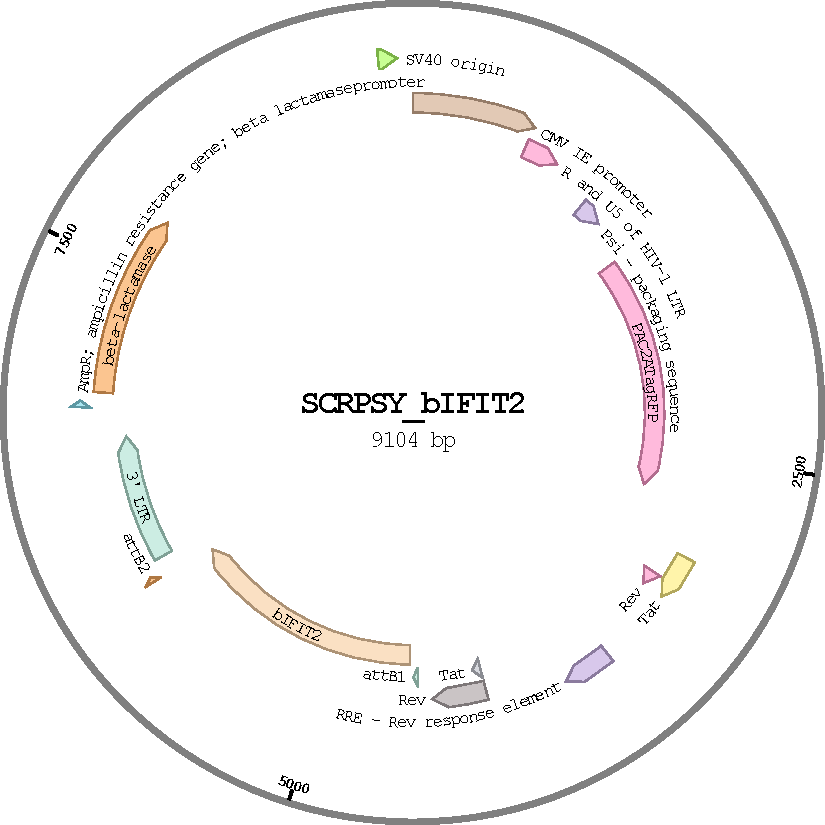
\includegraphics[width=0.6\linewidth]{05. Methods/Figs/01. scrpsy.pdf}
    \caption[SCRPSY Representative Map.]{\textbf{SCRPSY Representative Map.}}
    \label{fig:SCRPSY Representative Map}
\end{figure}

\begin{figure}
    \centering
    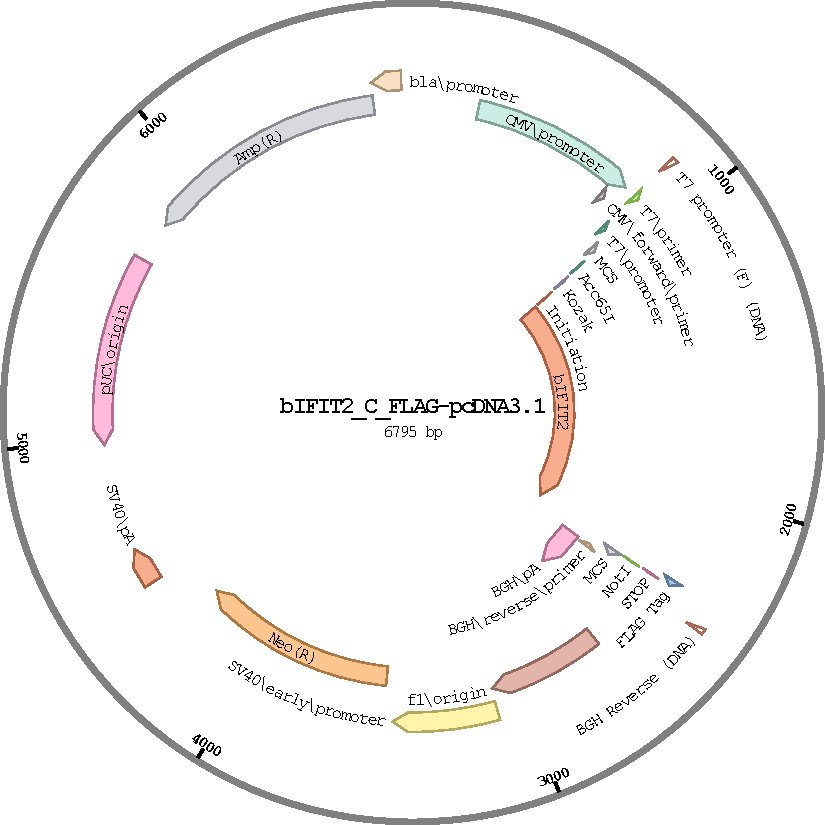
\includegraphics[width=0.6\linewidth]{05. Methods//Figs/02. pcDNA3.1.pdf}
    \caption[pcDNA3.1 Representative Map.]{\textbf{pcDNA3.1 Representative Map.}}
    \label{fig:pcDNA3.1 Representative Map}
\end{figure}




\subsection{Common Subcloning Methodologies} \label{subsec:Common Subcloning Methodologies}
\subsubsection[DNA Agarose Gel Electrophoresis and Extractions]{Analysis of DNA by Agarose Gel Electrophoresis and Gel Extractions} \label{Analysis of DNA by Agarose Gel Electrophoresis and Gel Extractions}
Linearised DNA was resolved and potentially isolated on 0.8\% agarose in Tris-Borate EDTA (TBE) buffer gel. 0.8\% agarose mixture was used as it provides resolution power greater than 10kbp-0.1kbp. DNA visualisation was enabled by the addition of 15 \(\mu\)L ethidium bromide into 50 mL agarose TBE solution at \~50°C prior to gel casting. DNA samples were mixed with 6X loading buffer (NEB) and loaded onto the gel. A DNA ladder was also electrophoresed in a separate well to allow size comparison. Samples were run at 80V for 90 minutes. After the run DNA bands were visualised using UV. Samples intended for gel purifications were excised from the gel using a clean scalpel and were placed into clean 1.5 mL tubes.




\subsubsection{DNA Clean-Up After PCR or Gel Extraction} \label{DNA Clean-Up After PCR or Gel Extraction}
DNA clean-up was performed using QiaQuick Gel Extraction kit (Quiagen) with accordance to the manufacturers protocol. In short, 3 volumes of buffer QC were added to either post PCR DNA or to a gel slice (where 1 mg of gel was assumed to be equivalent to 1 \(\mu\)L). Samples were incubated at 50°C for 10 minutes, after which one sample volume of isopropanol was added to the samples. Samples were collected on a QIAquick spin column via centrifugation and washed with buffer PE twice. DNA was eluted to 1.5 mL tube using centrifugation.




\subsubsection{DNA Ligation} \label{DNA Ligation}
20 \(\mu\)L total volume ligation reaction was prepared using DNA to be ligated, 2 \(\mu\)L T4 DNA ligase buffer (NEB) and 1 \(\mu\)L of T4 DNA ligase (NEB). Samples were incubated at 16°C for 72 hours.




\subsubsection[Transformation of \textit{E.Coli} and Bacterial Culture]{Transformation of Chemically Competent \textit{E.Coli} Cells and Bacterial Culture Amplification} \label{Transformation of Chemically Competent E.Coli Cells and Bacterial Culture Amplification}
2 \(\mu\)L of ligated samples or 1 \(\mu\)L of concentrated DNA were mixed with 25 \(\mu\)L \textit{E. coli} in 0.5 mL PCR tubes and were placed in a PCR cycler. Samples were initially incubated at 4°C for 15 minutes, following by heat shock performed by incubation at 42°C for 45 seconds followed by 2 minutes at 4°C. Afterwards, 75 \(\mu\)L of SOC solution was added and samples were left to incubate at 37°C for 60 minutes. Finally, 100 \(\mu\)L of transformed bacterial culture was streaked on room temperature agar plate containing ampicillin with a quadrant streaking method to ensure dilution gradient establishment on the plate allowing for single colony formation in the final quadrant. Plates were left to incubate for 24 hours at 37°C. Afterwards, single colonies were picked, annotated, and amplified in LB broth containing 1 \(\mu\)L per mL of ampicillin for 24 hours at 37°C.




\subsubsection{DNA Purification and Sequencing} \label{DNA Purification and Sequencing}
Bacterial cultures from the final step of Section \ref{Transformation of Chemically Competent E.Coli Cells and Bacterial Culture Amplification} were pelleted by centrifugation at 4°C for 30 minutes at 4000 g. Based on the size of the culture, the plasmid DNA was purified either by Miniprep or Midiprep kit (Quiagen; from 5 mL and 50 mL cultures respectively) based on the manufacturers protocol using the alkaline lysis method. Final purified DNA was quality assessed by restriction digestion followed by agarose gel electrophoresis (described in Section \ref{Analysis of DNA by Agarose Gel Electrophoresis and Gel Extractions}), which, if successful, was followed by sanger sequencing. Sequencing primers used to sequence ORFs of pcDNA3.1 plasmids were the forward T7 promoter primer and reverse BGH primer.




\subsection{PCR for Cloning into pcDNA3.1} \label{subsec:PCR for Cloning into pcDNA3.1}
In order to create tagged bovine \textit{IFIT} ORFs and subclone them from SCRPSY backbone into pcDNA3.1 backbone the following protocol was used. Primers were designed based on the schematic in \ref{fig:Schematic for PCR Primer Design}. The primers were 27-60 nucleotides in length. Their melting temperatures were established and used in the PCR protocol. PCR reaction mixtures with final volume of 100 \(\mu\)L were created by combining 10 \(\mu\)L of 10X Pfu Buffer (Promega) with 100 ng of plasmid DNA, 4 \(\mu\)L of 5 nM dNTPs (NEB), 2 \(\mu\)L of Pfu DNA polymerase (Promega), 1 \(\mu\)L of 100 \(\mu\)M forward and reverse primer and nuclease-free water. Samples were placed in PCR thermocycler and incubated for 30 seconds at 98°C. Followed were 30 cycles of 10 seconds at 98°C, followed by 30 seconds at 58°C and 90 seconds at 72°C. Final step was incubation at 72°C for 2 minutes. To degrade the original plasmid material, samples were incubated with DpnI restriction enzyme for 1 hour at 37°C. Afterwards, samples were cleaned as described in Section \ref{DNA Clean-Up After PCR or Gel Extraction}. The ORF amplicons had their ends digested by a sequential restriction digest with Acc65I (NEB) and NotI (NEB) restriction enzymes. This was done by diluting samples with 10X 3.1 buffer into 1X, adding restriction enzyme, incubation for 1 hour at 37°C and heat inactivation of enzyme at 65°C for 15 minutes. Digested amplicons were cleaned-up as described in Section \ref{DNA Clean-Up After PCR or Gel Extraction}. Donor plasmid pcDNA3.1 was linearised using Acc65I and NotI restriction enzymes as described above, and gel extracted as detailed in Section \ref{Analysis of DNA by Agarose Gel Electrophoresis and Gel Extractions} and \ref{DNA Clean-Up After PCR or Gel Extraction}. Linearised plasmid was dephosphorylated using Antarctic phosphatase (NEB). Amplicons and dephosphorylated plasmid were ligated in 5:1 molar ratio as described in Secton \ref{DNA Ligation}.

\begin{figure}
    \centering
    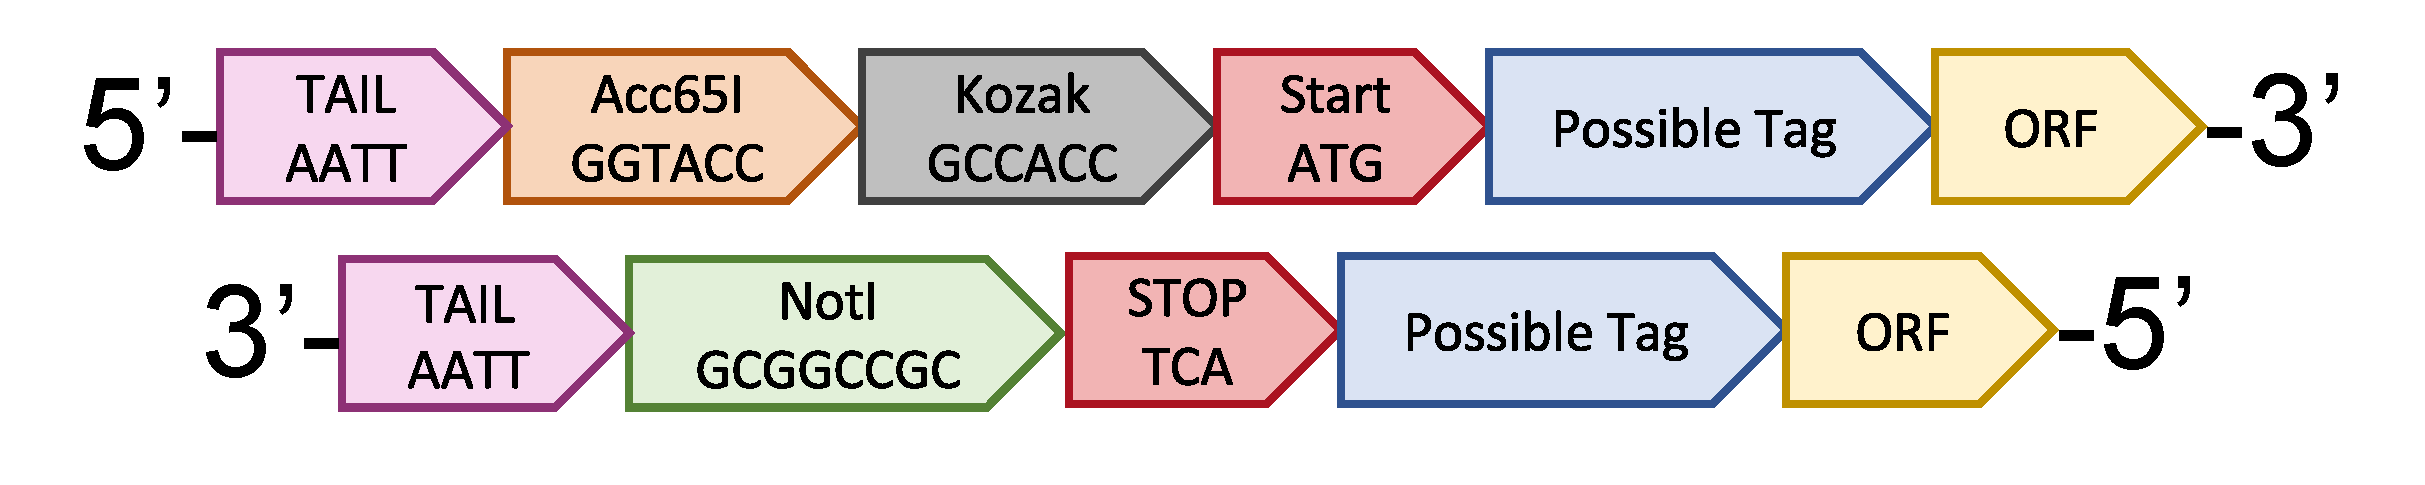
\includegraphics[width=1\linewidth]{05. Methods//Figs/03. cloning scheme.pdf}
    \caption[Schematic for PCR Primer Design.]{\textbf{Schematic for PCR Primer Design.}}
    \label{fig:Schematic for PCR Primer Design}
\end{figure}




\subsection{PCR for Point Mutant Generation} \label{subsec:PCR for Point Mutant Generation}
To create \textit{IFIT2} RNA-binding mutants a following protocol was used. Based on the publication in Tran \textit{et al.,} inverse PCR methodology was used with the primers for hIFIT mutations being taken from the study (\cite{Tran2020InfluenzaMRNAs}). bIFIT2 primers were based on the human ones. A protein model of human IFIT2 complex, visualised in PyMol software (\cite{SchrodingerTeam2023TheSystem}), had the amino acid residues 292 and 410 highlighted and compared to the residues on the corresponding place of predicted bovine IFIT2 structure. The effects of the mutations on the surfaces polarity assayed \textit{in silico}. This established that the corresponding amino acid residues on the bovine IFIT2 needed to be mutated were 287 and 401. The final primers can be seen in table Table \ref{tab:Primers for Inverse PCR Mutagenesis table}, where the mutating nucleotides are shown using lower case characters.
PCR reaction mixtures with final volume of 100 \(\mu\)L were created by combining 10 \(\mu\)L of 10X Pfu Buffer (Promega) with 100 ng of plasmid DNA, 4 \(\mu\)L of 5 nM dNTPs (NEB), 2 \(\mu\)L of Pfu DNA polymerase (Promega), 1 \(\mu\)L of 100 \(\mu\)M forward and reverse primer and nuclease-free water. Samples were placed in PCR thermocycler and incubated for 30 seconds at 98°C. Followed were 30 cycles of 10 seconds at 98°C, followed by 30 seconds at 58°C and 200 seconds at 72°C. Final step was incubation at 72°C for 2 minutes. To degrade the original plasmid material, samples were incubated with DpnI restriction enzyme for 1 hour at 37°C. Afterwards, samples were cleaned as described in Section \ref{DNA Clean-Up After PCR or Gel Extraction} and eluted in 20 \(\mu\)L of nuclease-free water. DNA was phosphorylated by adding 2\(\mu\)L of 10X ligase buffer and 1 \(\mu\)L of T4 Polynucleotide Kinase (NEB) and incubating the samples for 30 minutes at 37°C. The enzyme was inactivated by incubation at 65°C for 20 minutes. Samples were then ligated by addition of 1 \(\mu\)L of T4 DNA ligase and incubation at 16°C for 72 hours.

\begin{table}
\centering
\begin{tabular}{ll}
\hline
\textbf{Primer Name}   & \textbf{Sequence 5'-3'}    \\ \hline
hIFIT2   R292E forward & GTGCTGCTATgagGCAAAAGTCTTC  \\ \hline
hIFIT2 R292E reverse   & CCAATTTGGCAATGCAGG         \\ \hline
hIFIT2   K410E forward & GGAGAAAGAAgagATGAAAGACAAAC \\ \hline
hIFIT2 K410E reverse   & CTTGATTTCTGGTTTATTTTTACAC  \\ \hline
bIFIT2   R287E forward & GTGCTGCTATgagGCCAAAGTCCT   \\ \hline
bIFIT2 R287E reverse   & CCAATATGGCAATGCAGG         \\ \hline
bIFIT2   K401E forward & GAAGGAGAAgaaATGAAAAACAAAC  \\ \hline
bIFIT2 K401E reverse   & CTTTGATCCCTGGTTTAT         \\ \hline
\end{tabular}
\caption[Primers for Inverse PCR Mutagenesis.]{\textbf{Primers for Inverse PCR Mutagenesis.}}
\label{tab:Primers for Inverse PCR Mutagenesis table}
\end{table}




\section{Protein Work} \label{sec:Protein Work}
\subsection{Immunoprecipitation} \label{subsec:Immunoprecipitation}
Immunoprecipitation (IP) and co-immunoprecipitation (co-IP) was performed to isolate specific proteins or protein complexes, respectively. 2,000,000 HEK293T cells were seeded in a 10 cm dish. For transfection experiments 7.7 \(\mu\)g of DNA was transfected as described in Section \ref{subsec:Transfecting Cells}. 24 hours post transfection cells, or at the terminal point of experiment cells were scraped and transferred into a 50 mL conical tube. Cells were repeatedly spun down and washed with PBS until there was no residual contamination from culture media. Final cell pellet was resuspended in 1 mL of cold lysis buffer (10 mM Tris/HCl pH 7.5; 150 mM NaCl; 0.5 mM EDTA; 0.5\% NP-40; 1:100 protease inhibitors (Sigma)) and incubated for 30 minutes on ice. Afterwards samples were spun down at 20,000 g for 10 min at 4°C and the supernatant was transferred into pre-cooled tube. Dynabead protein-G beads (ThermoFisher) were bind to a target antibody by combining 50 \(\mu\)L of magnetic beads with 5 \(\mu\)g of target antibody in 200 \(\mu\)L of PBS with Tween 20 for 10 minutes at room temperature. Afterwards, using a magnet, the supernatant was removed without removing the bead-antibody complexes. After the beads were resuspended in lysis buffer. After centrifuging the lysates were added to the beads and incubated using a rotor for 30 minutes at 4°C. Afterwards the samples were washed twice using magnetic rack and a wash buffer (10 mM Tris/HCl pH 7.5; 150 mM NaCl; 0.5 mM EDTA). After the final wash was removed the bead-sample complexes were resuspended in 45 \(\mu\)L 2x SDS loading buffer, incubated at 95°C for 5 minutes. Afterwards the samples were centrifuged at top speed for 2 minutes and the pellet was discarded. This was the \textbf{bound} sample, which contained the immunoprecipitated target, along with the antibody which was used to precipitate it. During the experiment two additional samples were aliquoted, each 50 \(\mu\)L in volume. First was after centrifugation of the lysates (\textbf{input} sample) and the second after incubation of lysates with the beads on rotor (\textbf{unbound} sample). Both of these samples were mixed 1:1 with 2x SDS loading buffer and boiled at 95°C for 5 minutes.




\subsection{SDS-PAGE and Western Blotting} \label{subsec:SDS-PAGE and Western Blotting}
At the end point of experiments with cells, the growth medium was removed, and the cells were washed with PBS. Cells were lysed in 1X Laemmli SDS sample buffer (Bio-Rad) supplemented with \(\beta\)-mercaptoethanol (Sigma) and denatured by boiling at 95°C for 5 minutes. Samples were run on 10\% SDS polyacrylamide gels. The running gel was prepared using 10-\% v/v polyacrylamide (Protogel), 0.39 M Tris pH 8.8, 0.1\% w/v SDS, 0.1\% w/v ammonium persulphate (APS) and 0.04\% w/v tetramethylethylenediamine (TEMED; Bio-Rad). The stacking gel consisted of 5\% v/v polyacrylamide, 0.13 M Tris pH 6.8, 0.1\% w/v SDS, 0.1\% w/v APS and 0.1\% w/v TEMED. PageRuler Plus prestained protein ladder (Thermo Scientific) was used as a molecular weight marker. Samples were run in a Mini-PROTEAN Tetra Vertical Electrophoresis Cell (BioRad) at 110 V for 120 minutes. Afterwards the proteins were transferred into polyvinylidene difluoride (PVDF) membranes (Bio-Rad) using the Trans-blot Turbo blotting system (Bio-Rad) with 1X transfer buffer (25 mM Tris, 192 mM glycine, pH 8.3; Bio-Rad) following the manufacturer’s instructions (30 min at 25 V). Afterwards the membranes were blocked by incubation with with 5\% (w/v) skimmed milk in PBS with 0.1\% Tween 20 (PBST) for an hour. Afterwards the membranes were washed several times with in PBS with 0.1\% Tween 20. During this step it is possible to reversible visualise proteins on the membrane using Ponceau S (ThermoFisher). After washing steps the membranes were incubated with milk-PBST-primary antibody mixtures overnight at 4°C, washed three times with PBS-T and probed with either horseradish peroxidase-conjugated secondary antibodies or fluorophore-conjugated secondary antibodies, diluted in 5\% milk in PBST. Protein bands were detected either directly or using Clarity Western ECL substrate (Bio-Rad) and imaged with Bio-Rad ChemiDoc MP Imaging System.




\section{Confocal Microscopy} \label{sec:Confocal Microscopy}
Cells grown on a glass coverslip with 13 mm diameter (Agar Scientific) were washed with PBS and fixed by incubating for 15 minutes with room temperature 4\% paraformaldehyde (Sigma-Aldrich) at the end point of the experiments. Samples were subsequently permeabilised by being incubated in 0.2\% Triton X-100/PBS solution for 5 minutes. Residual Triton was removed by PBS washes, after which the coverslips were blocked using 1\% bovine serum albumin (BSA; Sigma-Aldrich) in PBS for at least 30 minutes. Samples were then incubated overnight with the primary antibody 1\% BSA in PBS solution, diluted as specified in Table \ref{tab:Antibodies for Confocal Microscopy}. Afterwards, they were washed again with PBS and incubated for an hour at room temperature with secondary antibodies diluted in 1\% BSA in PBS solution, as specified in Table \ref{tab:Antibodies for Confocal Microscopy}. Nuclei of the cells were stained by 4,6-diamidino-2-phenylindole (DAPI; Abcam), diluted 1:20,000 in water. After 10-minute incubation, residual DAPI was washed away by water, following by an additional was with PBS. Stained slides were mounted on glass slides using Vectashield (Vector Labs). Confocal images were acquired on Leica TCS SP5 and Zeiss LMS700 confocal microscopes using 405 nm, 488 nm, and 568 nm laser lines with 63X oil immersion objective. Laser lines were operated in sequential manner to prevent bleed-through and the image quality was enhanced by frame averaging. The pinhole was set to 1 airy unit. Maximal laser line gains were established per experiment using secondary antibody only controls, while minimal gains were established using the maximum intensity of sample slides, allowing for maximum range of signal acquisition. Image analysis was conducted in FiJi (\cite{Schindelin2012Fiji:Analysis}) and final figures were constructed using QuickFigures FiJi plugin (\cite{Mazo2021QuickFigures:Figures}).


\begin{table}
\centering
\begin{tabular}{@{}cccc@{}}
\toprule
\textbf{Antibody Target} & \textbf{Host Species} & \textbf{Provider} & \textbf{Working Dilution} \\ \midrule
RSV N       & Mouse  & Abcam             & 1:400   \\
RSV P       & Mouse  & FILL              & 1:400   \\
RSV   M2/1  & Mouse  & FILL              & 1:400   \\
IFIT1       & Rabbit & Invitrogen        & 1:200   \\
IFIT2   (A) & Rabbit & Proteintech       & 1:200   \\
IFIT2 (B)   & Rabbit & Novus Biologicals & 1:200   \\
IFIT3       & Rabbit & Proteintech       & 1:200   \\
IFIT5       & Rabbit & Invitrogen              & 1:200   \\
FLAG        & Rabbit & Invitrogen              & 1:200   \\
Rabbit Igg  & FILL   & Invitrogen              & 1:10000 \\
Mouse   Igg & FILL   & Invitrogen              & 1:10000 \\ \bottomrule
\end{tabular}
\caption[Antibodies for Confocal Microscopy.]{\textbf{Antibodies for Confocal Microscopy.}}
\label{tab:Antibodies for Confocal Microscopy}
\end{table}




\section{RNAseq Differential Expression Analysis} \label{sec:RNAseq Differential Expression Analysis}
RNAseq experiments comparing the transcript levels between control cells and cells infected with either wild-type bovine RSV or bovine RSV with a deleted SH gene, either 16 and 40 hours post infection were previously performed by Dr. Fouthemata Jobe from the Viral Glycoproteins Group at the Pirbright Institute. The initial data analysis was performed by the bioinformatics team of the Pirbright Institute. They included the viral genes as a part of the analysis and therefore these were the only differentially expressed genes from the study. I have reanalysed the counts dataset, which had viral genes omitted. Data processing, statistical analysis and graph generation was conducted R programming language (\cite{RCoreTeam2022R:Computing}) using RStudio enviroment (\cite{RStudioTeam2022RStudio:RStudio}). Initial exploratory data analysis and differential expression analysis was done using the DESeq2 R package (\cite{Love2014ModeratedDESeq2}). Viral genes were filtered from the dataset pre analysis. After creation of DESeq2 object, genes with no counts were filtered. To perform initial exploratory data analysis and visualization data was transformed using regularized logarithm (rlog) and the variance stabilizing transformation (VST) methods. This was done to stabilize the variance across the mean. The transformed data was visualised using the principal component analysis (PCA) plot and sample distance matrix. Following this the differential expression analysis was performed on non-transformed filtered data. Following the recommendation of Schurch \textit{et al.}, the fold-change threshold was set to 0.5 and the minimum adjusted p value was set to 1\% to optimise the true positive rate and false positive rates (\cite{Schurch2016HowUse}). The data was visualised by volcano plots, MA plots and heatmaps (using pheatmap R package (\cite{Kolde2019Pheatmap:Heatmaps})). The final dataset was annotated with the appropriate gene names and gene symbols from latest available bovine genomic dataset using org.Bt.eg.db R package (\cite{Carlson2022Org.Bt.eg.db:Bovine}).




\section{Statistical Analysis} \label{sec:Statistical Analysis}
Statistical analysis was performed using R programming language (\cite{RCoreTeam2022R:Computing}) using the RStudio environment (\cite{RStudioTeam2022RStudio:RStudio}). The pipeline can be viewed in the following URL: http://rpubs.com/ogosimiso/995988. Initially, data was assessed visually using boxplots and Q-Q plots. Boxplots were used to roughly assess the normality, whereas Q-Q plots were used for rough equality of variance assumptions. A mathematical test of the normality of distribution was done using the Shapiro-Wilk normality test. This was performed on each individual condition as well as the whole dataset in its entirety. Mathematical assessment of equality of variance was done by Bartlett test of homogeneity of variances for normally distributed samples and by Levene's Test for Homogeneity of Variance (car package for R (\cite{Fox2019AnRegression})) for non-normally distributed samples. To obtain the final significance values various mathematical tests were used based on the number of comparisons and the previously established type of distribution and equality of variance. For a pair of samples with normal distribution and equal variance a two-sample t-test was conducted. For multiple comparisons of normally distributed data with equal variance analysis of variance (ANOVA) combined with Tukey multiple comparison of means was performed. For a pair of samples with non-normal distribution but equal variance, a two-sample t-test was conducted. For multiple comparisons of non-normally distributed data with equal variance a Kruskal-Wallis rank sum test was performed (dunn.test R package (\cite{Dinno2017Dunn.test:Sums})). For a single comparison of data which has normal distribution but non-equal variance a Welch Two Sample t-test was performed. For multiple comparisons of data with normal distribution but non-equal variance one-way analysis of means (not assuming equal variances) combined with Games-Howell test was performed (rstatix R package (\cite{Kassambara2022Rstatix:Tests})). 

%acronyms
\nomenclature[z-DMEM]{$DMEM$}{Dulbecco’s Modified Eagle’s Medium} 
\nomenclature[z-FBS]{$FBS$}{Foetal Bovine Serum }    
\nomenclature[z-PBS]{$PBS$}{Phosphate Buffered Saline}    
\nomenclature[z-IFN]{$IFN$}{Interferon}  
\nomenclature[z-ANOVA]{$ANOVA$}{Analysis of Variance} 
\nomenclature[z-PCA]{$PCA$}{Principal Component Analysis} 
\nomenclature[z-VST]{$VST$}{Variance Stabilizing Transformation} 
\nomenclature[z-rlog]{$rlog$}{Regularized Logarithm} 
\nomenclature[z-DAPI]{$DAPI$}{4,6-diamidino-2-phenylindole} 
\nomenclature[z-BSA]{$BSA$}{Bovine Serum Albumin} 
\nomenclature[z-PBST]{$PBST$}{PBS with 0.1\% Tween 20} 
\nomenclature[z-PVDF]{$PVDF$}{polyvinylidene difluoride} 
\nomenclature[z-TEMED]{$TEMED$}{tetramethylethylenediamine} 
\nomenclature[z-APS]{$APS$}{ammonium persulphate}  
\nomenclature[z-IP]{$IP$}{Immunoprecipitation}  
\nomenclature[z-co-IP]{$co-IP$}{co-immunoprecipitation}  
\nomenclature[z-TBE]{$TBE$}{Tris-Borate EDTA}  
\nomenclature[z-ORFs]{$ORFs$}{Open Reading Frames}  
\nomenclature[z-GFP]{$GFP$}{Green Fluorescent Protein}  
\nomenclature[z-MOI]{$MOI$}{Multiplicity of Infection}  
\nomenclature[z-PEG]{$PEG$}{Polyethylene Glycol}  
\nomenclature[z-cDNA]{$cDNA$}{Complementary DNA}  
\nomenclature[z-qPCR]{$qPCR$}{Quantitative Polymerase Chain Reaction}  
\nomenclature[z-Ct]{$Ct$}{Cycle Threshold}  
\nomenclature[z-MMLV RT]{$MMLV RT$}{Moloney Murine Leukaemia Virus Reverse Transcriptase}  

%Words in text: 4832
%Words in headers: 127
\chapter{Assesment of Transcriptional Induction, Expression, and Subcellular Localisation of Human IFITs in the Context of RSV} \label{Assesment of Transcriptional Induction, Expression, and Subcellular Localisation of Human IFITs in the Context of RSV}
\section{Introduction and Aims} \label{Introduction and Aims-Chapter 1}
\textbf{Half page intro:}
Ifit gene regulation (promoters and such) \newline
Ifit paths of induction \newline
interferons \newline
Lps tlr4 \newline
Poly IC \newline
Ifit induction by other viruses and inducers \newline


\textbf{Half page aims:}
We hypothesised both human and bovine IFITs to be induced by human and bovine RSV infection. We aimed to systematically test this by initially confirming that our model cell lines are capable of IFIT induction following the treatment of known innate immune system activators such as interferons, LPS, and poly I:C. These would also allow us to assess the  We would then assess the IFIT induction during human and bovine RSV infection using a range of viral concentrations and end assay time points. Lastly, we would validate this data in more physiologically relevant cell lines as well as using omics approaches.

\section{Results} \label{Results-Chapter 1}

\subsection{Transcriptional Changes of Human \textit{IFITs}} \label{Transcriptional Changes of Human IFITs}
To unravel the impact of cellular stimulation with activators of the innate immune response and human RSV, on the expression of human \textit{IFIT} genes, quantitative real-time reverse transcription PCR (qPCR) analysis was executed in accordance with the methodology outlined in Section \ref{Quantitative Real Time/Reverse Transcription PCR}. Briefly, cells were cultivated in 12-well plates and subsequently subjected to the respective stimulants. At the endpoint of the experiments, the RNA was extracted, followed by cDNA synthesis and the transcript quantification by qPCR. All transcript levels were standardized to human \textit{GAPDH} expression, employing  the 
\(\Delta\)\(\Delta\)Ct method. Subsequently, all values were normalized against mock-treated samples, enabling data aggregation and inter-experimental induction value comparison. The statistical analysis was conducted as outlined in Section \ref{Statistical Analysis}. Notably, the choice of the appropriate statistical test hinged on the normality of data distribution and equality of variance, aspects which will be underscored in the ensuing text.



\subsubsection{Human \textit{IFITs} Responses of to Known Activators of Innate Immune Response} \label{Human IFIT Responses to Known Activators of Innate Immune Response}
In order to establish the expression competency of human \textit{IFITs} of the A549 cell line, along with elucidating how different innate immune pathways contribute to the overall expression profile, I treated the cells with differing activators of the innate immune response. As described in Section \ref{Routes of IFIT Expression Activation}, and depicted in Figure \ref{Pathways Inducing ISG mRNA Production.},  interferon-stimulated genes (ISGs) can have their induction activated either via the interferon receptor signalling, intracellular foreign nucleic acid detection or via extracellular PAMP sensing. The latter, in the context of RSV, includes stimulation of TLR4 with either LPS or RSV particles. After surveying the literature I ended up using 1,000 international units (IU) per mL of human interferon alpha (\cite{Terenzi2006DistinctISG56}; \cite{Santhakumar2018ChickenViruses}). For interferon-gamma stimulation, which stimulates predominantly immune cells \textit{in vivo} concentrations of 500, 1,000 and 2,000 IU/mL were used. LPS was administered in concentrations of 5 ng/mL and 5 \(\mu\)g/mL for the duration of 6 hours. (\cite{Mears2019Ifit1Cells}; \cite{Zhang2019GrouperResponse}). To stimulate intracellular foreign nucleic acid recognition 2 \(\mu\)g of poly I:C were transfected into A549 cells and incubated for 24 hours (\cite{Mears2019Ifit1Cells}; \cite{Palchetti2015TransfectedCells}).

\begin{figure}
    \centering
    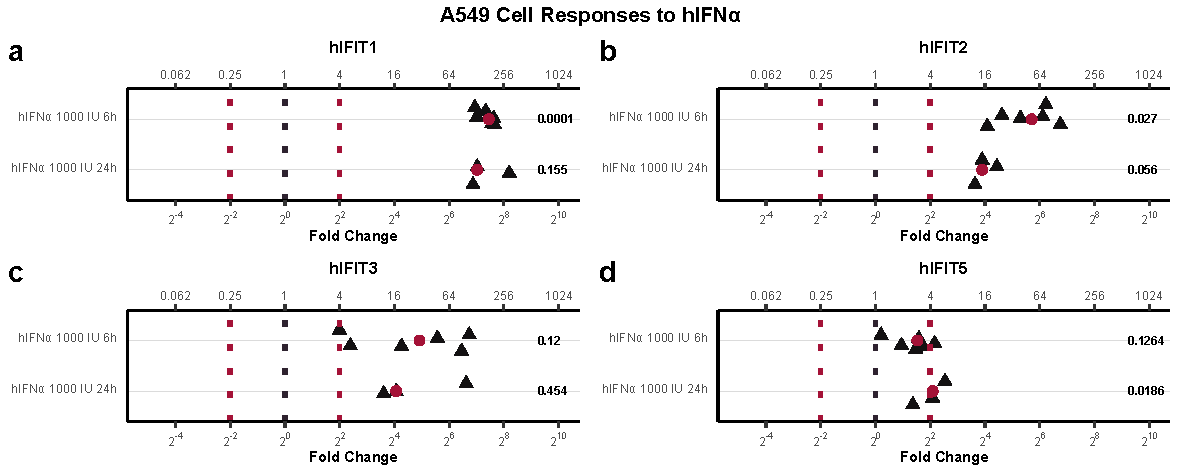
\includegraphics[width=1\linewidth]{06. Chapter 1/Figs/01. Induction/01. a549_treat_ifna.pdf}
    \caption[qPCR Analysis of A549 \textit{hIFIT} Response to hIFN\(\alpha\).]{\textbf{qPCR Analysis of A549 \textit{hIFIT} to hIFN\(\alpha\).} The relative abundance of (a) \textit{hIFIT1}, (b) \textit{hIFIT2}, (c) \textit{hIFIT3}, and (d) \textit{hIFIT5} genes, extracted from the A549 cell line, with response to human interferon alpha (IFN\(\alpha\)) at a concentration of 1000 IU per mL for a treatment duration of 6 or 24 hours. The shown values are relative to standardised mock values. The red circles signify median values. The black dotted line indicates mock expression, while the red dotted lines indicate biologically significant levels of induction. Numeric values signify the p-values compared to mock.}
    \label{A549 Response to hIFNa}
\end{figure}

The A549 cell line, derived from   lung carcinomatous tissue from a 58-year-old Caucasian male in 1972 is a well-established model of alveolar epithelial cells, routinely used for cancer to viral research alike (\cite{Lieber1976ACells}). We observe that after the stimulation of the A549 cell line with 1,000 IU/mL of hIFN\(\alpha\) for either 6 or 24 hours human \textit{IFIT1}, \textit{IFIT2}, and \textit{IFIT3} were induced drastically, especially \textit{IFIT1}, which was induced around 200-fold (Figure \ref{A549 Response to hIFNa}). The relative induction levels were identical between \textit{IFIT2} and \textit{IFIT3}. For all of these 3 genes, we can observe a decreased expression with longer incubation of IFN\(\alpha\), i.e. approximately half of the induction levels caused by 6-hour long incubation. Human \textit{IFIT5} shows minimal induction compared to the other \textit{IFITs} (3 and 4-fold for 6 and 24-hour long incubation respectively), which hovers around the mark of what is considered biologically significant induction, especially for ISGs, which are supposed not to be highly basally expressed. We can also observe a reverse trend of the time dependency of hIFN\(\alpha\)-induced expression. This suggests differential induction sensitivities between \textit{hIFIT1} (highly induced), \textit{hIFIT2} and \textit{hIFIT3} (medium induced) and \textit{hIFIT5} (low induced). All \textit{hIFIT} values had normal distributions and unequal variance other than \textit{hIFIT5}, which had normal distribution and normal variance.

\begin{figure}
    \centering
    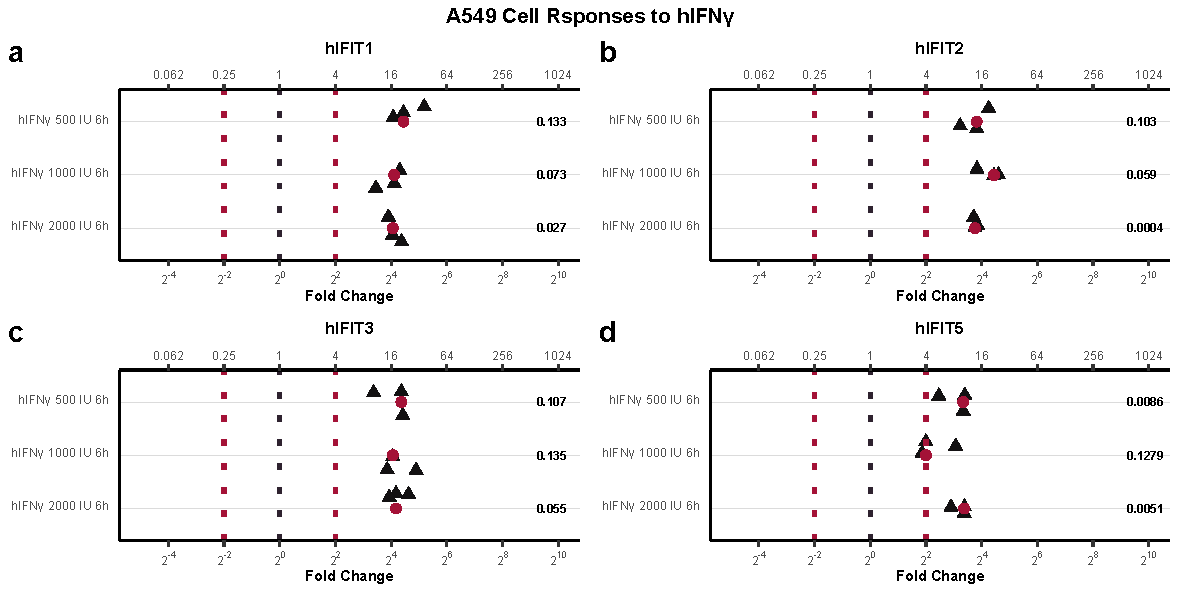
\includegraphics[width=1\linewidth]{06. Chapter 1/Figs/01. Induction/02. a549_treat_ifng.pdf}
    \caption[qPCR Analysis of A549 \textit{hIFIT} Response to hIFN\(\gamma\).]{\textbf{qPCR Analysis of A549 \textit{hIFIT} Response to hIFN\(\gamma\).} The relative abundance of (a) \textit{hIFIT1}, (b) \textit{hIFIT2}, (c) \textit{hIFIT3}, and (d) \textit{hIFIT5} genes, extracted from the A549 cell line, with response to human interferon-gamma (IFN\(\gamma\)) at concentrations of 500, 1000, and 2000 IU per mL for a treatment duration of 6 hours. The shown values are relative to standardised mock values. The red circles signify median values. The black dotted line indicates mock expression, while the red dotted lines indicate biologically significant levels of induction. Numeric values signify the p-values compared to mock.}
    \label{A549 Response to hIFNg}
\end{figure}

The response of human \textit{IFIT} genes to human IFN gamma can be seen in Figure \ref{A549 Response to hIFNg}. We can observe all \textit{IFITs} other than \textit{hIFIT5} responding equally to all concentrations tested i.e. 500, 1,000 and 2,000 IU/mL. Their response was concentration independent of a magnitude of around 15-fold. \textit{hIFIT5} response to very low concentration and very high concentrations was around 10-fold, while its transcript abundance increased only 4 times when treated with 1,000 IU/mL concentration. This suggests that the interferon-gamma component of the human \textit{IFIT} response is relatively equal for all of the \textit{IFIT} genes. This data, along with the data from hIFN\(\alpha\) induction also confirms that the A549 cell line is \textit{hIFIT} induction capable, which is great. All \textit{hIFIT} values had normal distributions and unequal variance other than \textit{hIFIT5}, which had normal distribution and normal variance.

\begin{figure}
    \centering
    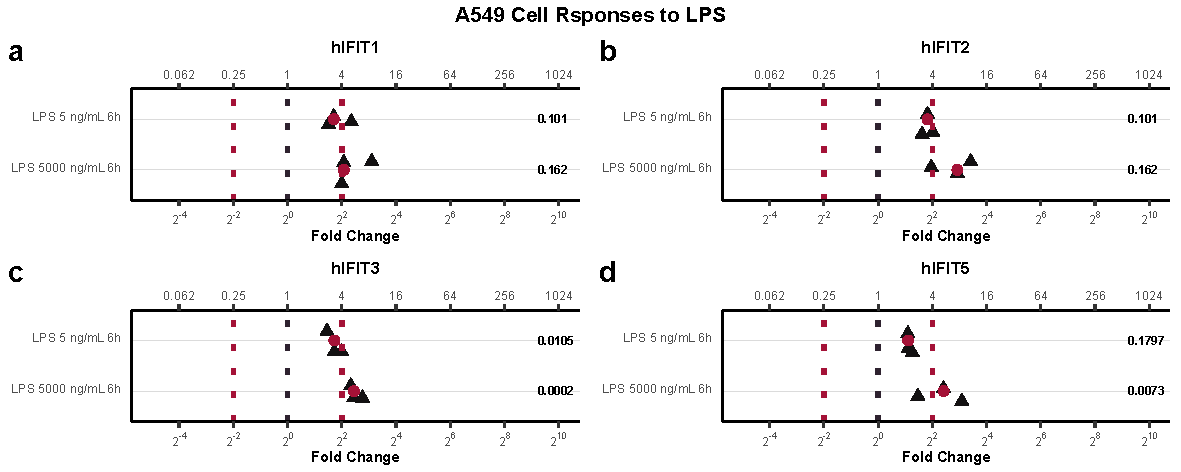
\includegraphics[width=1\linewidth]{06. Chapter 1/Figs/01. Induction/03. a549_treat_lps.pdf}
    \caption[qPCR Analysis of A549 \textit{hIFIT} Response to LPS.]{\textbf{qPCR Analysis of A549 \textit{hIFIT} Response to LPS.} The relative abundance of (a) \textit{hIFIT1}, (b) \textit{hIFIT2}, (c) \textit{hIFIT3}, and (d) \textit{hIFIT5} genes, extracted from the A549 cell line, with response to lipopolysaccharide (LPS) at concentrations of 5 and 5000 ng/mL for a treatment duration of 6 hours. The shown values are relative to standardised mock values. The red circles signify median values. The black dotted line indicates mock expression, while the red dotted lines indicate biologically significant levels of induction. Numeric values signify the p-values compared to mock.}
    \label{A549 Response to LPS}
\end{figure}

In order to assess the involvement of TLR4, a receptor also responsible for detecting RSV particles, A549 cells were incubated for 6 hours with low (5 ng/mL) and high (5,000 ng/mL) concentrations of bacterial LPS, its known activator. We can see that all \textit{IFITs} respond in a concentration dependant manner but the response is the lowest out of the different stimulants used. Low-concentration LPS incubation causes biologically insignificant induction of all \textit{hIFITs} of 2-fold for \textit{hIFIT5} and 3-fold for the other \textit{IFITs}. The high concentration on the other hand yields biologically significant induction levels of 4-8 fold induction. All \textit{hIFIT} values had normal distributions and unequal variance other than \textit{hIFIT3}, which had normal distribution and normal variance.

\begin{figure}
    \centering
    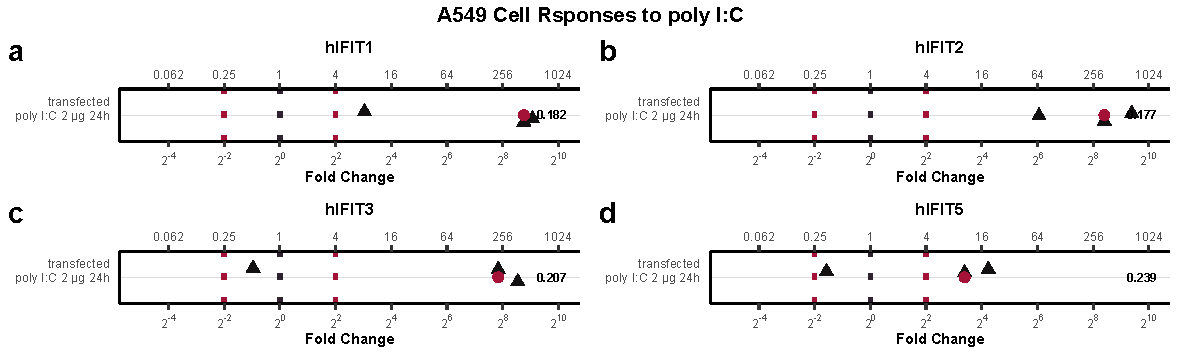
\includegraphics[width=1\linewidth]{06. Chapter 1/Figs/01. Induction/04. a549_treat_polyic.pdf}
    \caption[qPCR Analysis of A549 \textit{hIFIT} Response to Transfected poly I:C.]{\textbf{qPCR Analysis of A549 \textit{hIFIT} Response to Transfected poly I:C.} The relative abundance of (a) \textit{hIFIT1}, (b) \textit{hIFIT2}, (c) \textit{hIFIT3}, and (d) \textit{hIFIT5} genes, extracted from the A549 cell line. The cells were transfected with 2 \(\mu\)g of poly I:C for 24 hours. The shown values are relative to standardised mock values. The red circles signify median values. The black dotted line indicates mock expression, while the red dotted lines indicate biologically significant levels of induction. Numeric values signify the p-values compared to mock.}
    \label{A549 Response to poly I:C}
\end{figure}

When A549 cells were transfected with 2\(\mu\)g of poly I:C for 24 hours we were able to observe the biggest induction compared to the other inducers previously used (Figure \ref{A549 Response to poly I:C}). As with the other inducers, hIFIT1 induction is the greatest (circa 500-fold), followed by \textit{hIFIT2} and \textit{hIFIT3} with 300-fold and 200-fold responses respectively, with \textit{hIFIT5} trailing behind with the lowest response of only 10-fold. This again suggests that \textit{hIFIT5} seems to have differential transcriptomic regulation compared to the other genes of the \textit{IFIT} family. All \textit{hIFIT} values had normal distributions and unequal variance.

\begin{figure}
    \centering
    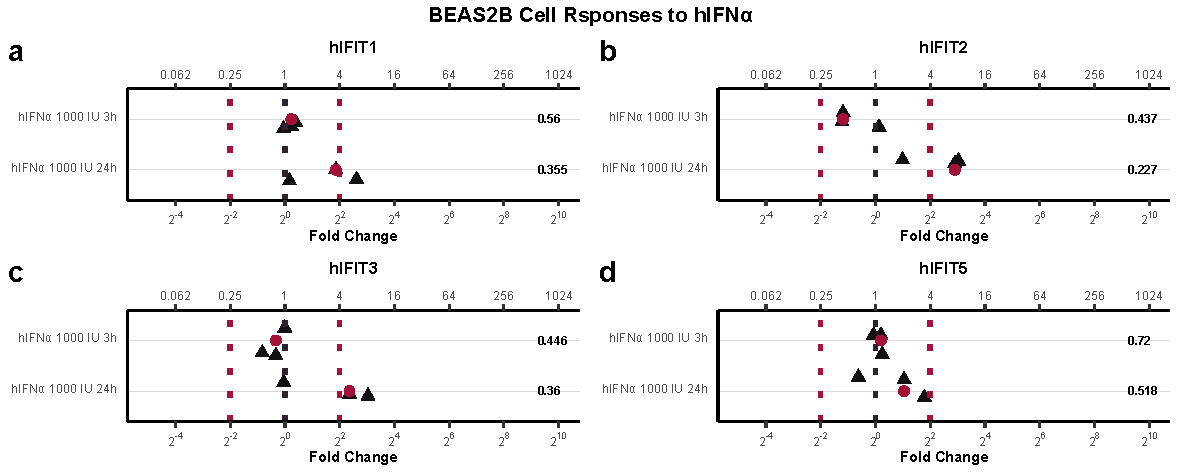
\includegraphics[width=1\linewidth]{06. Chapter 1/Figs/01. Induction/09. beas2b_ifna.pdf}
    \caption[qPCR Analysis of BEAS-2B \textit{hIFIT} Response to hIFN\(\alpha\).]{\textbf{qPCR Analysis of BEAS-2B \textit{hIFIT} Response to hIFN\(\alpha\).} The relative abundance of (a) \textit{hIFIT1}, (b) \textit{hIFIT2}, (c) \textit{hIFIT3}, and (d) \textit{hIFIT5} genes, extracted from the BEAS-2B cell line, with response to human interferon alpha (IFN\(\alpha\)) at a concentration of 1000 IU per mL for a treatment duration of 3 or 24 hours. The shown values are relative to standardised mock values. The red circles signify median values. The black dotted line indicates mock expression, while the red dotted lines indicate biologically significant levels of induction. Numeric values signify the p-values compared to mock.}
    \label{BEAS-2B responses to hIFNa}
\end{figure}

Lastly, we validated the human interferon alpha induction data in a more biologically relevant cell line, BEAS-2B. Established from bronchial epithelial biopsies from healthy samples, and later immortalised using the transfection of cyclin-dependent kinase 4 and human telomerase reverse transcriptase, these cells are an invaluable tool in the field of bronchial development and pathogenesis (\cite{Ramirez2004ImmortalizationOncoproteins}). After the treatment with human interferon alpha at concentrations of 1,000 IU/mL for 3 hours, we can see that this stimulation was not sufficient to induce the expression of any human \textit{IFIT} (Figure \ref{BEAS-2B responses to hIFNa}). However, when the cells were stimulated for 24 hours we can observe induction above biological significance for \textit{hIFIT1}, \textit{hIFIT2}, and \textit{hIFIT3}, with 4-fold, 8-fold, and 5-fold increase respectively. \textit{hIFIT5} shows only 2-fold median induction, which could be caused by the intrinsic variability of the assay. So as we observed with the A549 cell line, \textit{hIFIT5} behaves in discord with the other human \textit{IFITs}. All \textit{hIFIT} values had normal distributions and unequal variance.


\subsubsection{Human \textit{IFITs} Responses to Human RSV Infection} \label{Human \textit{IFITs} Responses to Human RSV}
After successfully confirming the \textit{IFIT} induction competency of  our workhorse cell line A549 as well as in the more physiologically relevant cell line BEAS-2B, we turn our attention to assessing the effect of human RSV infection on \textit{hIFIT} induction. To date, no studies have ever investigated this. Initially, we wanted to assess the effect of low, medium and high (0.1, 1, and 2 MOI respectively) infections as well as short and long-term infections (24 and 48 HPI respectively) on \textit{hIFIT} induction. My colleagues in the Viral Glycoproteins from the Pirbright Institute routinely perform hRSV infections of both A549 and BEAS-2B cell lines and thus the knowledge of what constitutes low and high MOI infection, as well as what short and long infection periods are widely known and available (I GUESS SOME CITATION HERE).  The virus was prepared and quantified as described in Section \ref{Virus Propagation and Production} and Section \ref{Virus Quantification by TCID50 Assay}. Briefly, infected cells were sonicated, cell debris was separated by centrifugation and virus-containing supernatant was gathered and titred. A549 cells were infected with the hRSV-containing supernatant at multiplicities of infection (MOI) of 0.1, 1,  and 2. Total mRNA was collected from the samples either 24 or 48 hours post-infection (HPI) and converted to complementary DNA, as described in Section \ref{RNA Extraction and cDNA Synthesis}. This was subsequently quantified by qPCR as described in Section \ref{Quantitative PCR} and the data analysed as described in Section \ref{Data Processing}. The responses of \textit{hIFITs} as a function of HPI and MOI can be seen in Figure \ref{A549 response to hRSV timepoints}, along with a plot quantifying human \textit{RSV N} mRNA as a control for viral replication. The relative quantification values of \textit{RSV N} has to be taken with a grain of salt as it is being compared to mock-infected samples that should have no \textit{RSV N} mRNA present. As a result, the actual relative values are dependent on the Ct values detected in the mock. 
 

\begin{figure}
    \centering
    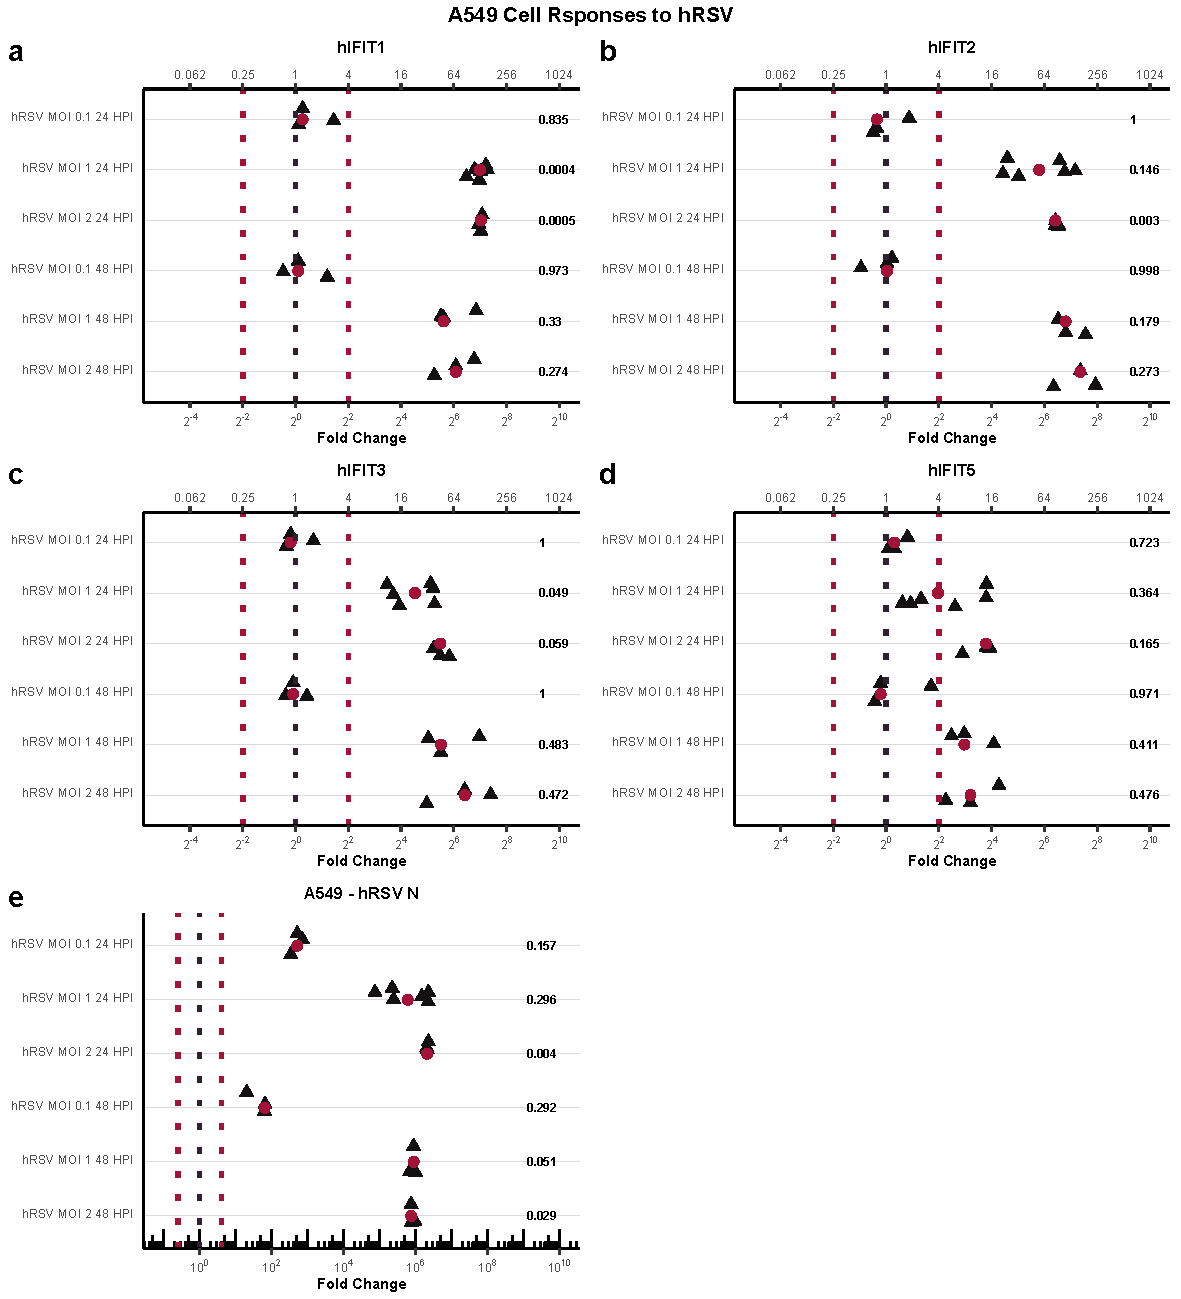
\includegraphics[width=1\linewidth]{06. Chapter 1/Figs/01. Induction/05. a549_hrsv_timepoints.pdf}
    \caption[A549 \textit{hIFIT} Response to hRSV as a Function of Time and MOI.]{\textbf{A549 \textit{hIFIT} Response to hRSV as a Function of Time and MOI.} The relative abundance of (a) \textit{hIFIT1}, (b) \textit{hIFIT2}, (c) \textit{hIFIT3}, (d) \textit{hIFIT5}, and (e) \textit{hRSV N} genes, extracted from A549 cell line following infection with human RSV at MOI of either 0.1, 1, or 2 for either 24 or 48 hours post-infection. The shown values are relative to standardised mock values. The red circles signify median values. The black dotted line indicates mock expression, while the red dotted lines indicate biologically significant levels of induction. Numeric values signify the p-values compared to mock.}
    \label{A549 response to hRSV timepoints}
\end{figure}


First of all, we can observe low MOI infection, although causing a productive infection as seen by \textit{hRSV N} mRNA relative quantification, did not yield any relative change of \textit{hIFIT} levels, suggesting that their induction is dependant not solely on the viral replication, but on the underlying magnitude of infection. In general, MOI 2 infection yields higher induction for all \textit{hIFITs}, although the magnitude is comparable with MOI 1 infections. \textit{hIFIT1} is induced the highest out of the other genes at 24 HPI, with both MOI 1 and 2 reaching 120-fold induction levels, while the induction magnitude diminishes slightly at 48 HPI, where infections at MOI 1 and 2 yield 50-fold and 80-fold median induction values. As seen previously in Section \ref{Human IFIT Responses to Known Activators of Innate Immune Response}, \textit{hIFIT2} and \textit{hIFIT3} display very similar trends of induction (with the only difference being \textit{hIFIT2} responses being 2 times the ones of \textit{hIFIT3}) for all the conditions tested here. In more detail, 24 HPI \textit{hIFIT2} gets induced 60-fold and 90-fold to the MOI of 1 and 2 respectively, while at 48 HPI the median induction magnitude increases to 100-fold and 120-fold respectively. This makes \textit{hIFIT2} the highest induced \textit{hIFIT} at 48 HPI. This also suggest that the induction dynamics of \textit{hIFIT1} differ from those of \textit{hIFIT2} and \textit{hIFIT3}. With regards to \textit{hIFIT5}, it displays the lowest, albeit still biologically significant induction for MOIs 1 and 2 for both time-points tested at median induction levels of 4 and 12 for 24 HPI MOIs 1 and 2 respectively, and 9 and 10 for 48 HPI MOIs 1 and 2 respectively. All datasets were of normal distribution and non-equal variance.


\begin{figure}
    \centering
    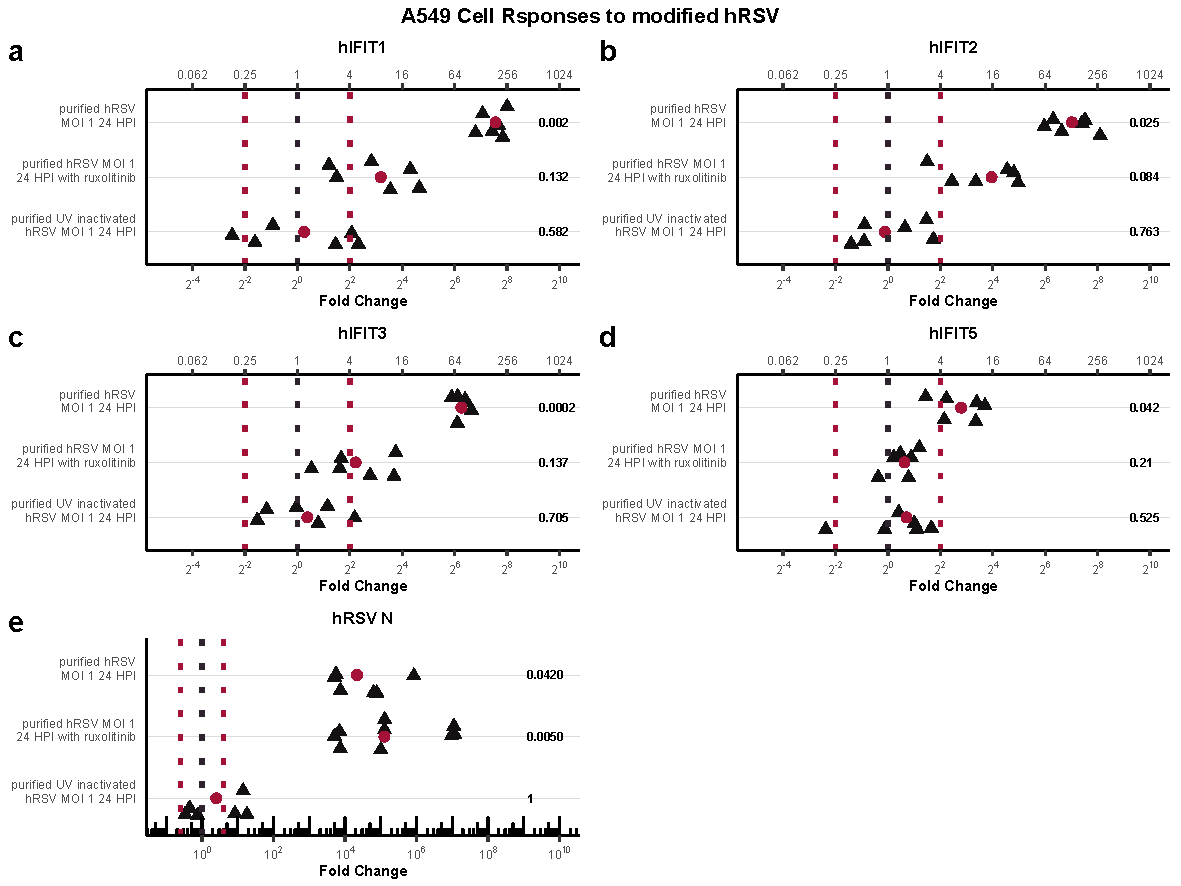
\includegraphics[width=1\linewidth]{06. Chapter 1/Figs/01. Induction/06. a549_hrsv_uv_roxo.pdf}
    \caption[The Effect of Ultra-Purification, UV-Inactivation and INFR Inhibition on \textit{hIFIT} Induction Following hRSV Infection in A549.]{\textbf{The Effect of Ultra-Purification, UV-Inactivation and INFR Inhibition on \textit{hIFIT} Induction Following hRSV Infection in A549.} The relative abundance of (a) \textit{hIFIT1}, (b) \textit{hIFIT2}, (c) \textit{hIFIT3}, (d) \textit{hIFIT5}, and (e) \textit{hRSV N} genes, extracted from A549 cell line following infection with ultra-purified hRSV at MOI 1 for 24 hours. The cells were either treated with the virus alone (first row), or with the virus and 5 nM of ruxolitinib (interferon receptor inhibitor) during the whole infection period (second row), or with UV-inactivated hRSV (last row). The shown values are relative to standardised mock values. The red circles signify median values. The black dotted line indicates mock expression, while the red dotted lines indicate biologically significant levels of induction. Numeric values signify the p-values compared to mock.}
    \label{The effect of ultra-purification, UV-inactivation and INFR inhibition on hIFIT induction following hRSV infection in A549}
\end{figure}

After confirming and concluding that human RSV infection indeed induces \textit{hIFIT} mRNA expression, we wanted to investigate the underlying induction principles. We wanted to investigate if the induction observed is indeed caused by human RSV detection and not by any other contaminants present in the virus prep such as cytokines, chemokines, and other stimulants. To do this, we created ultra-purified hRSV preps by ultra-centrifugation on a discontinuous sucrose cushion, as described in Section \ref{Virus Propagation and Production}. We also wanted to test if it is predominately the infected cells that have the \textit{hIFIT} expression increased as a defence mechanism to acute infection, or if the infected cells stimulate the \textit{hIFIT} expression in neighbouring cells as a prophylactic against the infection, or both. To test this, after the infection procedure, we incubated the cells with 5 nM of ruxolitinib, a well established small molecule JAK/STAT inhibitor, as is described in Section \ref{Viral Infections, UV-Inactivation and Ruxolitinib Treatment}. Based on the observations from Figure \ref{A549 response to hRSV timepoints} we used MOI of 1, 24 HPI to ensure sufficient \textit{hIFIT} induction, while decreasing the stress of the cells.  Lastly, we also hypothesised that viral replication is required for \textit{hIFIT} expression. To test this, some ultra-purified hRSV samples were UV-inactivated by a UV-cross-linker, as described in Section \ref{Viral Infections, UV-Inactivation and Ruxolitinib Treatment}.

The results of the experiment can be seen in Figure \ref{The effect of ultra-purification, UV-inactivation and INFR inhibition on hIFIT induction following hRSV infection in A549}. \textit{hRSV N} dataset was of normal distribution with equal variance, while all the other were of normal distribution and non-equal variance. We can see that although purified hRSV infection yielded lower induction compared to what was observed in Figure \ref{A549 response to hRSV timepoints} with regards to hRSV MOI 1 24 HPI infection (\(10^6\)-fold to \(10^{4.5}\)-fold), it induced all \textit{hIFITs}, even to higher mounts that what was seen with crude-extracted virus. In more detail, \textit{hIFIT1} was induced the highest at 180-fold (compared to 120-fold observed previously), closely followed by \textit{hIFIT2}, which median induction was at 180-fold (compared to 80-fold observed previously). \textit{hIFIT3} induction was 75-fold, double what was seen previously with crude extracted hRSV, while \textit{hIFIT5} median induction was 6-fold, a very comparable level to 4-fold that was observed previously. Regardless of the absolute magnitude of the relative values, this data suggest that the main driving force in hRSV presence and not contaminants in the viral prep. With regards to the effect of JAK/STAT inhibitor ruxolitinib, its presence diminished induction of all \textit{hIFITs}. \textit{hIFIT1}, \textit{hIFIT2}, and \textit{hIFIT3} maintained median induction values above the biologically significant threshold at 8, 10, and 5-fold respectively, while \textit{hIFIT5} showed only minimal median induction value of only 1.5-fold. We can also observe an order of magnitude more \textit{hRSV N} mRNA detection, suggesting that inhibiting interferon signalling is beneficial for the virus, which makes sense. Lastly, we assessed how a detection of non-replicative hRSV particles contribute to \textit{hIFIT} induction. UV-cross-linking of hRSV inhibited viral replication, as can be seen by the {hRSV N} mRNA quantification. This in fact prevented induction of all the \textit{hIFITs}, suggesting that TLR4 sensing of RSV particle is not sufficient to initiate signalling cascades that would lead to \textit{hIFIT} induction. All together, this data suggest that hRSV particles indeed drive the \textit{hIFIT} induction, however, they have to be replication competent. Additional essential aspect is the presence of functional interferon signalling cascades and the underlying paracrine interferon signalling initiated by infected cells in order to protect its neighbours.

\begin{figure}
    \centering
    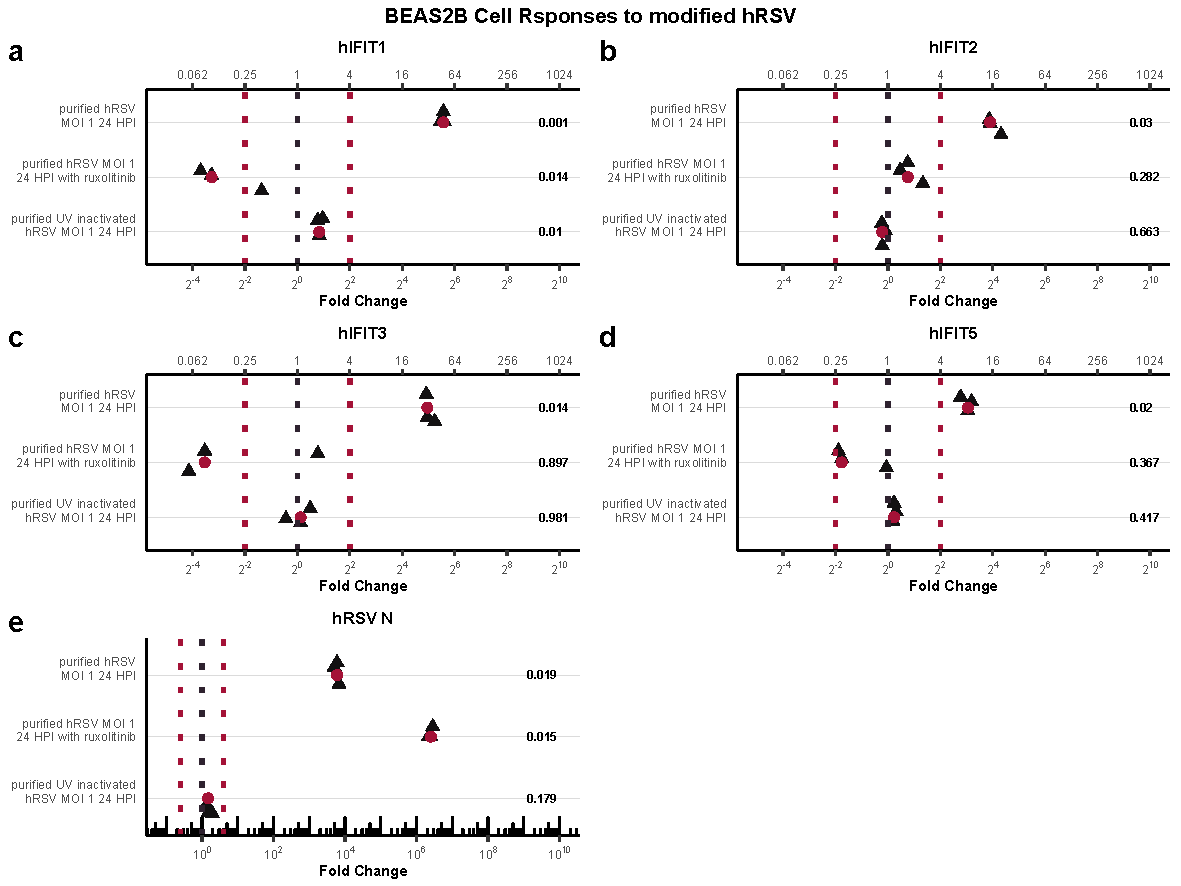
\includegraphics[width=1\linewidth]{06. Chapter 1/Figs/01. Induction/10. beas2b_hrsv.pdf}
    \caption[The Effect of Ultra-Purification, UV-Inactivation and INFR Inhibition on \textit{hIFIT} Induction Following hRSV Infection in BEAS-2B.]{\textbf{The Effect of Ultra-Purification, UV-Inactivation and INFR Inhibition on \textit{hIFIT} Induction Following hRSV Infection in BEAS-2B.} The relative abundance of (a) \textit{hIFIT1}, (b) \textit{hIFIT2}, (c) \textit{hIFIT3}, (d) \textit{hIFIT5} and (e) \textit{hRSV N} genes, extracted from BEAS-2B cell line following infection with ultra-purified hRSV at MOI 1 for 24 hours. The cells were either treated with the virus alone (first row), or with the virus and 5 nM of ruxolitinib (interferon receptor inhibitor) during the whole infection period (second row), or with UV-inactivated hRSV (last row). The shown values are relative to standardised mock values. The red circles signify median values. The black dotted line indicates mock expression, while the red dotted lines indicate biologically significant levels of induction. Numeric values signify the p-values compared to mock.}
    \label{The effect of ultra-purification, UV-inactivation and INFR inhibition on hIFIT induction following hRSV infection in BEAS-2B}
\end{figure}

Next we validated the findings using BEAS-2B cell line. We recreated the experiment from Figure \ref{The effect of ultra-purification, UV-inactivation and INFR inhibition on hIFIT induction following hRSV infection in A549} and the results can be seen in Figure \ref{The effect of ultra-purification, UV-inactivation and INFR inhibition on hIFIT induction following hRSV infection in BEAS-2B}. All datasets were of normal distribution and non-equal variance. All \textit{hIFITs} are induced to biologically significant levels by the infection of ultra-purified hRSV infection by 40, 15, 32, and 7-fold for \textit{hIFIT1}, \textit{hIFIT2}, \textit{hIFIT3}, and \textit{hIFIT5} respectively. These responses are also significantly higher than what was observed with human interferon alpha treatment (Figure \ref{BEAS-2B responses to hIFNa}). In line to what we have seen in A549 cell line, \textit{hIFIT1} is the highest induced, while \textit{hIFIT5} responds the worst to the infection. Interestingly, \textit{hIFIT3} median induction is higher than the one of \textit{hIFIT2}. When looking at the effect of ruxolitinib we can see that it prevented the induction of \textit{hIFIT2} and actually significantly decreased the relative levels of \textit{hIFIT1}, \textit{hIFIT3}, and \textit{hIFIT5} to the levels of \(2^{-3}\), \(2^{-3.5}\), and \(2^{-2}\) respectively. This suggest that not only is the interferon signalling required for \textit{hIFIT2} induction, it is vital for the maintenance  of basal \textit{hIFIT1}, \textit{hIFIT3}, and \textit{hIFIT5} levels in this cell line. Lastly, when the cells were infected with UV irradiated ultra-purified hRSV, none of the \textit{hIFITs} relative expression changed to biologically significant levels. This is in line to what we observed with A549 cell line. Taken together, we validate that replication competent viral particles are required for \textit{hIFIT} induction and while functional interferon receptor signalling cascades as also required, as we have seen in A549, in BEAS-2B they are necessary for maintaining the basal expression levels of \textit{hIFIT1}, \textit{hIFIT3}, and \textit{hIFIT5} mRNA levels.


\begin{figure}
    \centering
    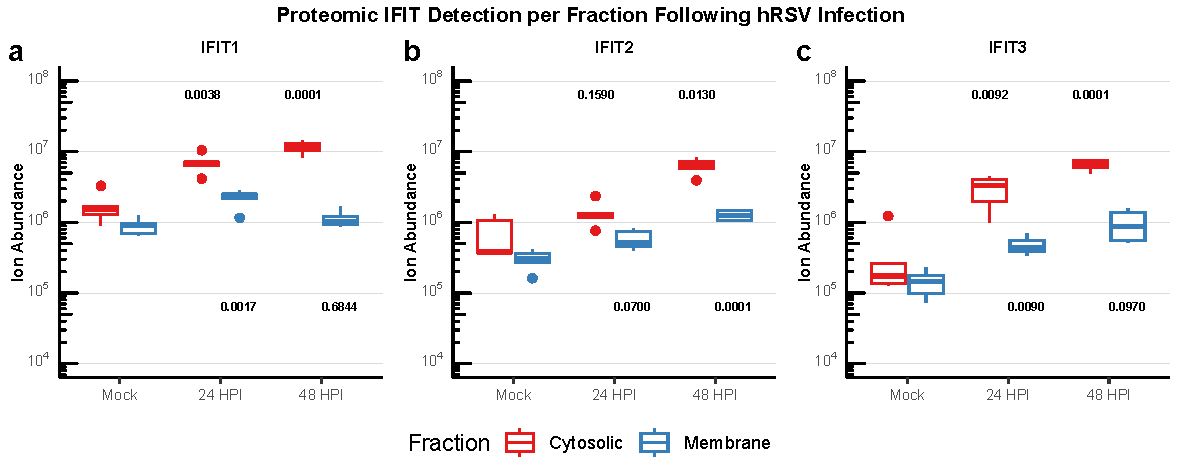
\includegraphics[width=1\linewidth]{06. Chapter 1/Figs/01. Induction/13. merged_proteomics.pdf}
    \caption[Human IFIT proteins detected per fraction.]{\textbf{Human IFIT proteins detected per fraction.} Analysis of summed peptide intensities of (a) hIFIT1, (b) hIFIT2, and (c) hIFIT3 detected per either cytosolic or membrane fractions of A549 cells which were either mock-infected, or infected with hRSV MOI 1 for either 24 or 48 hours.There were no hits for IFIT5. This data is from a proteomic study, published in \cite{Jobe2023ViralCondensates}. Samples are composed of biological quintuplicates. Numeric values signify the p-values compared to mock the respective mock, i.e. top numbers for cytosolic fraction, bottom for membrane fraction.}
    \label{Human IFIT proteomics.}
\end{figure}

To conclude the assessment of human IFIT responses to human RSV, I was kindly provided by a quantitative mass spectrometry dataset of human IFITs detected in either cytosolic or membrane fraction of either mock-infected or cells infected with human RSV at MOI 1, processed 24 or 48 HPI. This dataset was provided by Dr. Kelly and Dr. Jobe from the Pirbright Institute and its findings have now been published (\cite{Jobe2023ViralCondensates}). Quintuplicate of cytosolic and membrane fractions were isolated by in-gel digestion and analysed by label free quantitative mass spectrometry. Normalised and log transformed ion abundance data for hIFIT1, hIFIT2, and hIFIT3 can be seen in Figure \ref{Human IFIT proteomics.}. hIFIT1 cytoplasmic and hIFIT2 membrane datasets had normaldistributions and equal variances, while all the others displayed normal distributions with non-equal variances. Human IFIT5 did not yield any hits and thus was excluded from the analysis and we can conclude that its proteome is not drastically changed by hRSV infection, with is in line with our qPCR data. hIFIT1 is the most basally abundant, followed by hIFIT2 and hIFIT3. The basal abundance of hIFITs is around equal between the fractions. The infection at 24 HPI causes increased abundance of all hIFITs in all fraction, more specifically hIFIT1 increased 5x in cytosolic fraction and 1.3x in membrane fraction; hIFIT2 increased 4x in cytosolic and 2xin membrane fractions; and hIFIT3 increased relatively the most by 13.5x in cytosolic fraction and 3x in membrane fraction. The highest total abundance at 24 HPI was still hIFIT1. At 48 HPI we can observe further increase in abundance for all other than hIFIT1 in membrane fraction which decreased to mock levels. In more detail, hIFIT1 in cytosolic fraction increased further 2x; hIFIT2 increased further 5x in cytosolic and 4x in membrane fraction; and hIFIT3 further increased 3x in cytosolic fraction and 2.5x in membrane fraction. These data together validate our qPCR results seen in Figure \ref{A549 response to hRSV timepoints} and Figure \ref{The effect of ultra-purification, UV-inactivation and INFR inhibition on hIFIT induction following hRSV infection in A549} and highlight the differential spatio-temporal expression dynamics of human IFITs.


\subsubsection{Human \textit{IFITs} Responses to bRSV Infection} \label{Human IFITs Responses to bRSV}
We were interested knowing if there is cross-species protection between hRSV and bRSV, with regards to cell infectivity and \textit{hIFIT} induction. We had an arsenal of several bRSV viruses including the wild-type (WT) along with a panel of mutant viruses with deletions of small-hydrophobic (SH) protein, non-structural (NS) protein 1 or 2 or both (see Table \ref{Outline of Viruses Used table}). As described in INTRODUCTION these proteins are responsible for STUFF FROM INTRODUCTION. The viruses were prepared and quantified as described in Section \ref{Virus Propagation and Production} and Section \ref{Virus Quantification by TCID50 Assay}. Briefly, infected cells were sonicated, cell debris was separated by centrifugation and virus-containing supernatant was gathered and titred. It is to be noted that due to the lack of the anti-antiviral proteins meant the virus preparation of \(Delta\)NS viruses had orders of magnitude lower titre than the other viruses. Regardless, A549 cells were initially infected with the WT and \(Delta\)SH bRSV-containing supernatant at MOI of 1. Total mRNA was collected from the samples 24 HPI and converted to complementary DNA, as described in Section \ref{RNA Extraction and cDNA Synthesis}. This was subsequently quantified by qPCR as described in Section \ref{Quantitative PCR} and the data analysed as described in Section \ref{Data Processing}. The responses of \textit{hIFITs} as a function of HPI and MOI can be seen in Figure \ref{Responses of A549 to bRSV WT and dSH.}, along with a plot quantifying bovine \textit{RSV N} mRNA as a control for viral replication.

\begin{figure}
    \centering
    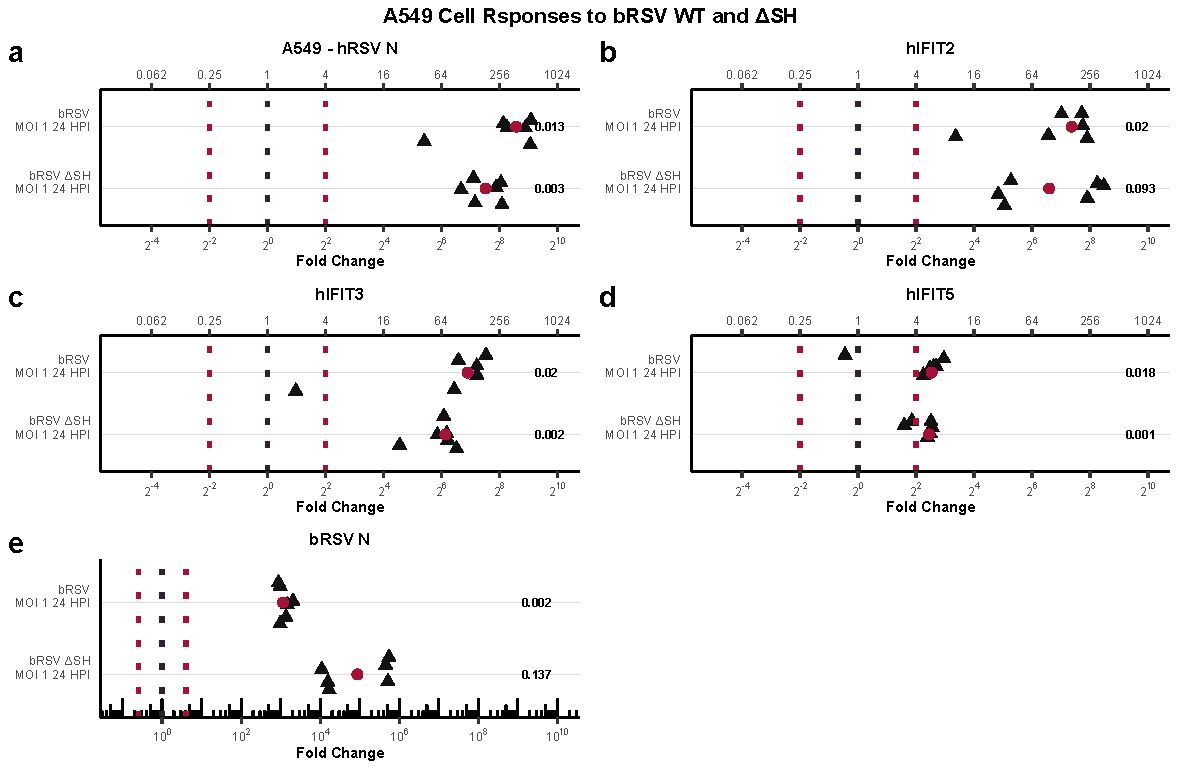
\includegraphics[width=1\linewidth]{06. Chapter 1/Figs/01. Induction/07. a549_brsv_moi1.pdf}
    \caption[A549 \textit{hIFIT} Response to WT and \(\Delta\)SH bRSV Infection.]{\textbf{A549 \textit{hIFIT} Response to WT and \(\Delta\)SH bRSV Infection.} The relative abundance of (a) \textit{hIFIT1}, (b) \textit{hIFIT2}, (c) \textit{hIFIT3}, (d) \textit{hIFIT5} and (e) \textit{bRSV N} genes, extracted from A549 cell line following infection with WT or \(\Delta\)SH bRSV at MOI 1, 24 HPI.  The shown values are relative to standardised mock values. The red circles signify median values. The black dotted line indicates mock expression, while the red dotted lines indicate biologically significant levels of induction. Numeric values signify the p-values compared to mock.}
    \label{Responses of A549 to bRSV WT and dSH.}
\end{figure}

We can see that both bRSV WT and bRSV \(\Delta\)SH were successfully replicating in the A549 cell line and this in fact both induced all \textit{hIFITs} to biologically significant levels. Interestingly, although bRSV \(\Delta\)SH \textit{N} relative mRNA levels were two orders of magnitude higher than the ones of WT bRSV, the detected indution magnitudes of \textit{hIFITs} were in general lower compared to the ones caused by bRSV WT infection. This is counterintuitive as the lack of SH protein should make the virus less infectious and thus show worse replication competency, while it should allow higher \textit{ISG} induction as there is less antagonism of the activation cascades present. Regardless, looking at the \textit{hIFITs} in more detail, \textit{hIFIT1} median induction by bRSV WT and \(\Delta\)SH infection was 400-fold and 150-fold respectively, which were again the highest induction magnitudes detected out of all \textit{hIFIT} response. On the other side of the spectrum is \textit{hIFIT5} with the median induction of 6-fold for both viruses, which are the lowest induction values and are consistent with what we observed so far throught the study. \textit{hIFIT2} was induced 180-fold and 80-fold by the WT and \(\Delta\)SH, while \textit{hIFIT3} was induced 128 and 70 fold respectively. Intriguingly, when compared to crude-extracted hRSV MOI 1 24 HPI from Figure \ref{A549 response to hRSV timepoints} we can see that although \textit{bRSV N} median relative abundances were two and one orders of magnitude lower for bRSV WT and \(\Delta\)SH respectively compared to \textit{hRSV N} but regardless, they caused greater induction of all \textit{hIFITs}. This suggest that bRSV is potentiated in human cells, probably due to the lack of species-specific inhibition, and this potentiation in turn causes higher \textit{hIFIT} induction as a response.

\begin{figure}
    \centering
    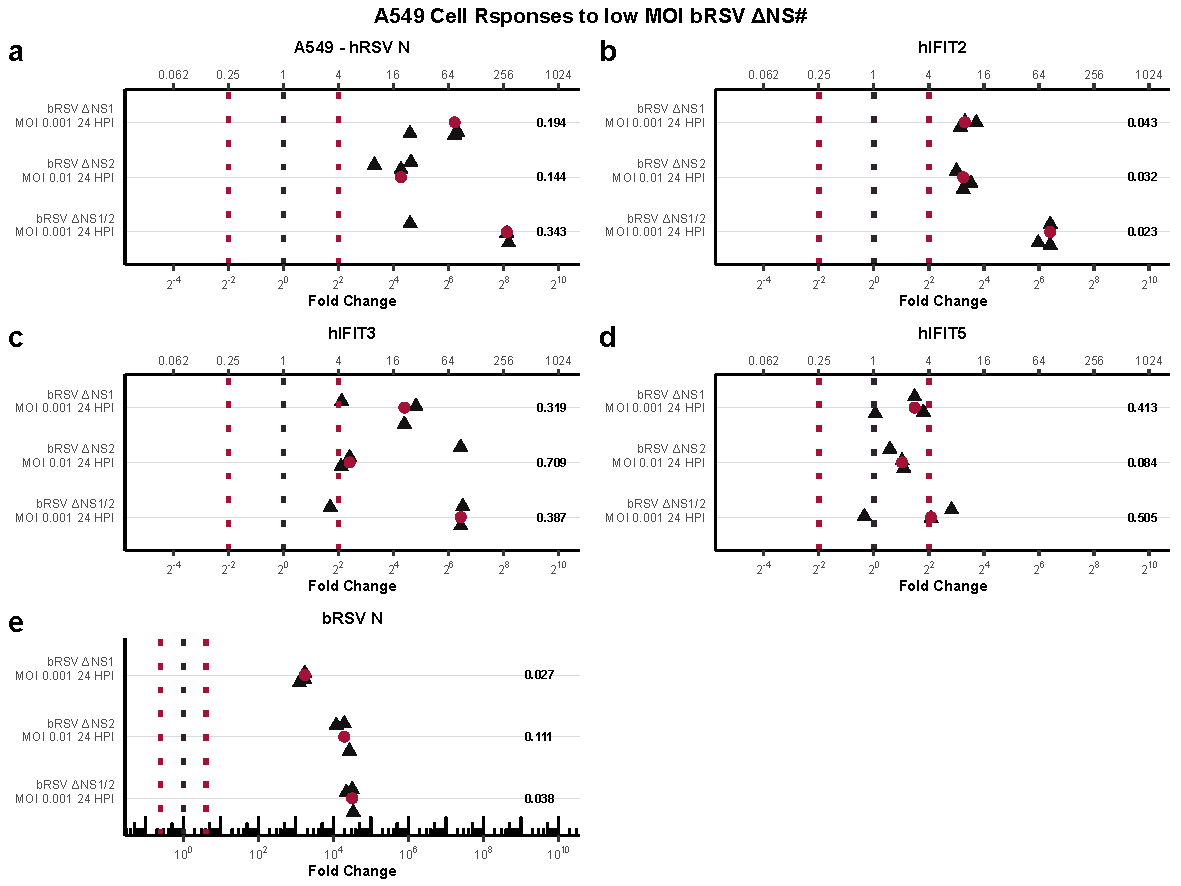
\includegraphics[width=1\linewidth]{06. Chapter 1/Figs/01. Induction/08. a549_brsv_dns.pdf}
    \caption[A549 \textit{hIFIT} Response to Low MOI \(\Delta\)NSs bRSV Infection.]{\textbf{A549 \textit{hIFIT} Response to Low MOI \(\Delta\)NSs bRSV Infection.} The relative abundance of (a) \textit{hIFIT1}, (b) \textit{hIFIT2}, (c) \textit{hIFIT3}, (d) \textit{hIFIT5} and (e) \textit{bRSV N} genes, extracted 24 HPI from A549 cell line following infection with bRSV \(\Delta\)NS1, \(\Delta\)NS2, and \(\Delta\)NS1/2 at MOIs of 0.001, 0.01, and 0.001 respectively. The shown values are relative to standardised mock values. The red circles signify median values. The black dotted line indicates mock expression, while the red dotted lines indicate biologically significant levels of induction. Numeric values signify the p-values compared to mock.}
    \label{Responses of A549 to bRSV dNSs.}
\end{figure}

Next, we investigated the effect of the rest of the mutant bRSV viruses, namely \(\Delta\)NS1, \(\Delta\)NS2, and a double knock-out \(\Delta\)NS1/2. As mentioned above, we had trouble achieving high titres using the crude-extraction methodology and thus the MOIs used are lower than what was conducted with WT and \(\Delta\)SH bRSV, more precisely 0.001 for \(\Delta\)NS1 and \(\Delta\)NS1/2, and 0.01 for \(\Delta\)NS2 bRSV. Total mRNA was extracted 24 hours post infection. In Figure \ref{Responses of A549 to bRSV dNSs.} we can see that all 3 viruses were able to successfully replicate, despite the low MOI. The replication magnitude mimics what was seen in Figure \ref{Responses of A549 to bRSV WT and dSH.} where \(\Delta\)NS1 \textit{bRSV N} mRNA levels were comparable to the wild-type infection and \(\Delta\)NS2 and \(\Delta\)NS1/2 levels were comparable to \(\Delta\)SH bRSV infection, although slightly lower. We can also observe mixed responses of \textit{hIFITs}, albeit all of them upregulation. \textit{hIFIT1} again was upregulated the highest, 70-fold, 20-fold and 300-fold to \(\Delta\)NS1, \(\Delta\)NS2, and \(\Delta\)NS1/2 respectively. \textit{hIFIT2} induction levels were almost identical for \(\Delta\)NS1 and \(\Delta\)NS2 viruses at around 8-fold despite the difference in MOI. \(\Delta\)NS1/2 bRSV infection induced it the highest, 70-fold. For \textit{hIFIT3} we can observe different induction dynamics. While \(\Delta\)NS1 infection induced it to higher levels that what we observed in \textit{hIFIT2} (20-fold), \(\Delta\)NS2 yielded barely biologically significant induction (4-fold), while virus lacking both non structural proteins induced \textit{hIFIT3} to equal levels as was observed with \textit{hIFIT2} (70-fold). Although we can see similar upregulation trends with \textit{hIFIT5} to what was observed with other \textit{hIFITs}, meaning \(\Delta\)NS1 causes medium induction, \(\Delta\)NS2 causes low induction, and \(\Delta\)NS1/2 causing high inducion, only the latter can be considered biologicaly significant (4-fold). Yet again, compared to the results with low MOI infection with hRSV (Figure \ref{A549 response to hRSV timepoints}), bRSV seems to be more replication competent, as seen by the relative \textit{bRSV N} mRNA levels, and a more potent \textit{hIFIT} inducer, as low MOI hRSV infection did not yield any induction what so ever. This data also highlights that NS1 negatively regulates \textit{hIFIT} induction more compared NS2, and a lack of both proteins seems to have a synergistic effect on \textit{hIFIT} induction.


\begin{figure}
    \centering
    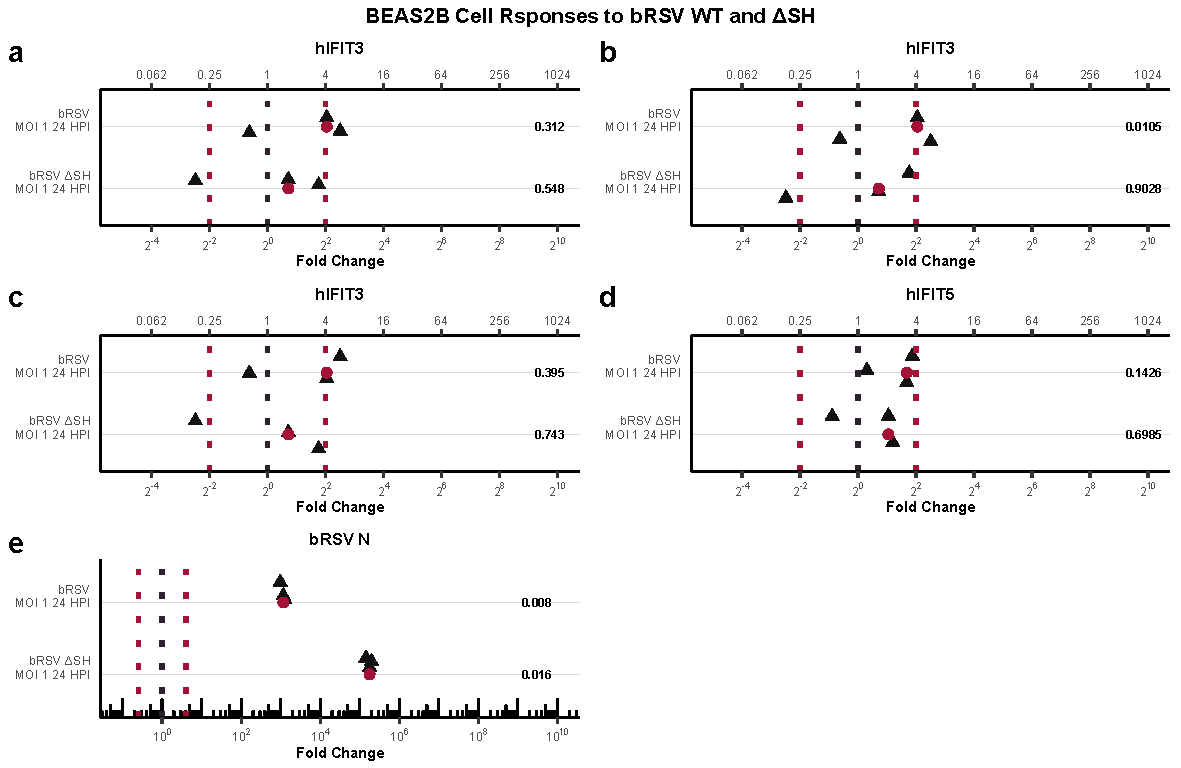
\includegraphics[width=1\linewidth]{06. Chapter 1/Figs/01. Induction/11. beas2b_brsv_moi1.pdf}
    \caption[BEAS-2B \textit{hIFIT} Response to WT and \(\Delta\)SH bRSV Infection.]{\textbf{BEAS-2B \textit{hIFIT} Response to WT and \(\Delta\)SH bRSV Infection.} The relative abundance of (a) \textit{hIFIT1}, (b) \textit{hIFIT2}, (c) \textit{hIFIT3}, (d) \textit{hIFIT5} and (e) \textit{bRSV N} genes, extracted from BEAS-2B cell line following infection with WT or \(\Delta\)SH bRSV at MOI 1, 24 HPI.  The shown values are relative to standardised mock values. The red circles signify median values. The black dotted line indicates mock expression, while the red dotted lines indicate biologically significant levels of induction. Numeric values signify the p-values compared to mock.}
    \label{BEAS-2B responses to bRSV WT and dSH.}
\end{figure}


Lastly we wanted to validate these results in BEAS-2B cell line. The experimental setup was identical to what was described above during the investigation of A549 \textit{hIFIT} responses to bRSV infection. Figure \ref{BEAS-2B responses to bRSV WT and dSH.} shows the induction levels caused by infection at MOI 1, 24 HPI with WT and \(\Delta\)SH bSRV. We can see, based on the median relative \textit{bRSV N} mRNA levels, that the viruses are capable of infecting BEAS-2B and are replicating approximately to the levels of what we observed in A549 cell line. We can also observe that the general trend from A549 one experiment is present, meaning \textit{hIFITs} are being positively induced, and more by the WT bRSV infection than the (\Delta\)SH one, with the difference being magnitude of these inductions. In more detail, the induction of all \textit{hIFITs} seems to be similar, barely biologically significant by WT infection (4-fold), and very weak by (\Delta\)SH infection (>2-fold). \textit{hIFIT5} is induced just below biological significance by WT bRSV and at the same level as the other \textit{hIFITs} by the mutant virus. So interestingly the \textit{hIFIT} induction seems to be cell line and stimulus specific.


\begin{figure}
    \centering
    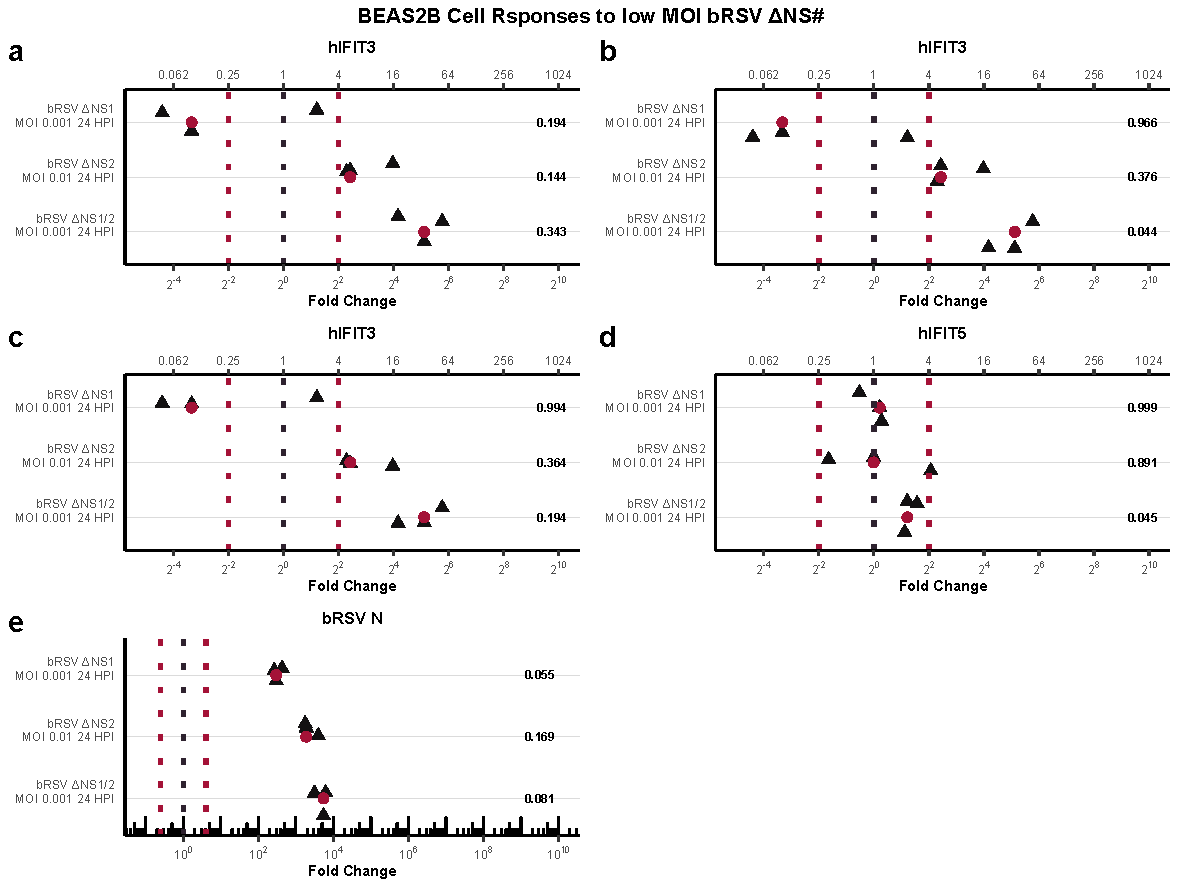
\includegraphics[width=1\linewidth]{06. Chapter 1/Figs/01. Induction/12. beas2b_brsv_dns.pdf}
    \caption[BEAS-2B \textit{hIFIT} Response to Low MOI \(\Delta\)NSs bRSV Infection.]{\textbf{BEAS-2B \textit{hIFIT} Response to Low MOI \(\Delta\)NSs bRSV Infection.} The relative abundance of (a) \textit{hIFIT1}, (b) \textit{hIFIT2}, (c) \textit{hIFIT3}, (d) \textit{hIFIT5} and (e) \textit{bRSV N} genes, extracted 24 HPI from BEAS-2B cell line following infection with bRSV \(\Delta\)NS1, \(\Delta\)NS2, and \(\Delta\)NS1/2 at MOIs of 0.001, 0.01, and 0.001 respectively. The shown values are relative to standardised mock values. The red circles signify median values. The black dotted line indicates mock expression, while the red dotted lines indicate biologically significant levels of induction. Numeric values signify the p-values compared to mock.}
    \label{BEAS-2B responses to bRSV dNSs.}
\end{figure}


Furthermore we validated the \(\Delta\)NSs infection data from A549 (Figure \ref{Responses of A549 to bRSV dNSs.}) using the same experimental setup as was described prevously. As we can see in Figure \ref{BEAS-2B responses to bRSV dNSs.}, the induction behaviour again differs from what we observed with A549 cell line. Based on \textit{bRSV N} mRNA levels, we can see that the mutant viruses were able to replicate, although the asolute relative values are one order of magnitude lower to what was observed with A549 cell line. \textit{hIFIT5} does not respond to the infection with \(\Delta\)NS1 and \(\Delta\)NS2 bRSv and positively but biologically significantly responds to \(\Delta\)NS1/2 virus. \textit{hIFIT1}, \textit{hIFIT2}, and \textit{hIFIT3} display very similar induction profile to the stimulant. More specificaly, \(\Delta\)NS1 infection downregulated all by \(2^{-3}\)-fold, while \(\Delta\)NS2 infection caused just biologically significant induction (4-fold), and the double mutant \(\Delta\)NS1/2 caused median induction of 32-fold. This data suggest NS1 protein being \textit{hIFIT} inductive, while the presence NS2 negatively influencing \textit{hIFIT} expression. This is in reverse to what we observed with A549. A lack of both non structural proteins seems to have synergisticly positive effect on \textit{hIFIT} induction, like we observed with the A549 cell line.

\subsubsection*{Summary} \label{Summary-human-induction}
Interestingly, the maximal induction of \textit{hIFIT5} observed in this study seems to be 10-16 fold, a order of magnitude lower of what is observed for the other \textit{hIFIT}.
\subsection{Localisation of Human and Bovine IFITs} \label{Localisation of Human and Bovine IFITs}
Asdfasfsdfasdf \newline
IF Mock | INF | Infection \newline
A549 BEAS2B

Merge pictures of clusters of cells looking at changes between subcellular localisation and a clear increase in mean intensity. Graphs show mean intensity changes from all cells imaged.

\begin{figure}
    \centering
    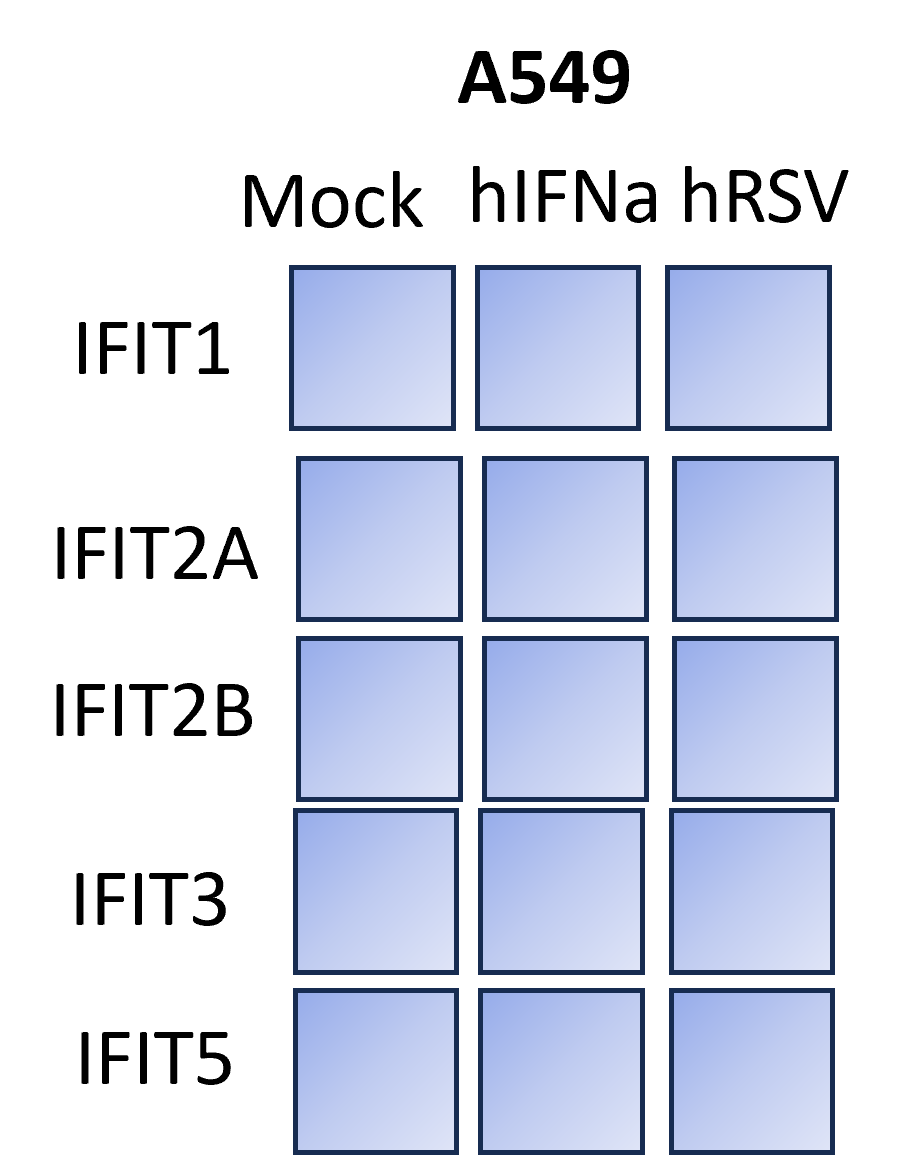
\includegraphics[width=1\linewidth]{06. Chapter 1/Figs/02. Localisation/01. a549 merges.png}
    \caption[A549 localisation mergers.]{A549 localisation mergers.}
    \label{A549 localisation mergers.}
\end{figure}


\begin{figure}
    \centering
    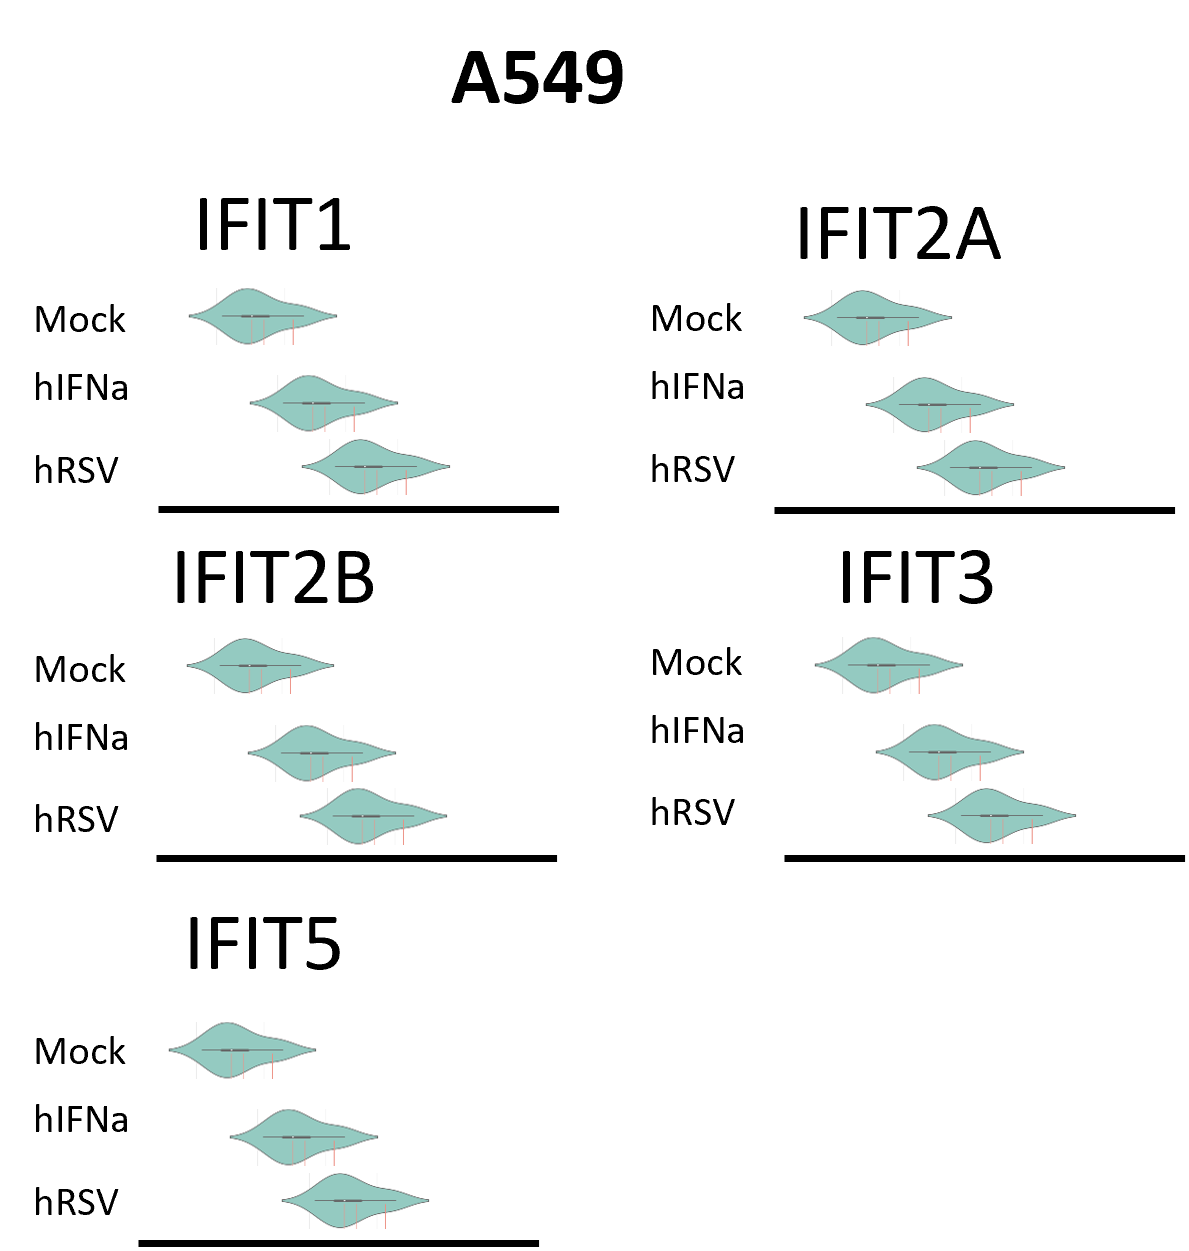
\includegraphics[width=1\linewidth]{06. Chapter 1/Figs/02. Localisation/02. a549 plots.png}
    \caption[A549 localisation plots.]{A549 localisation plots.}
    \label{A549 localisation plots.}
\end{figure}


\begin{figure}
    \centering
    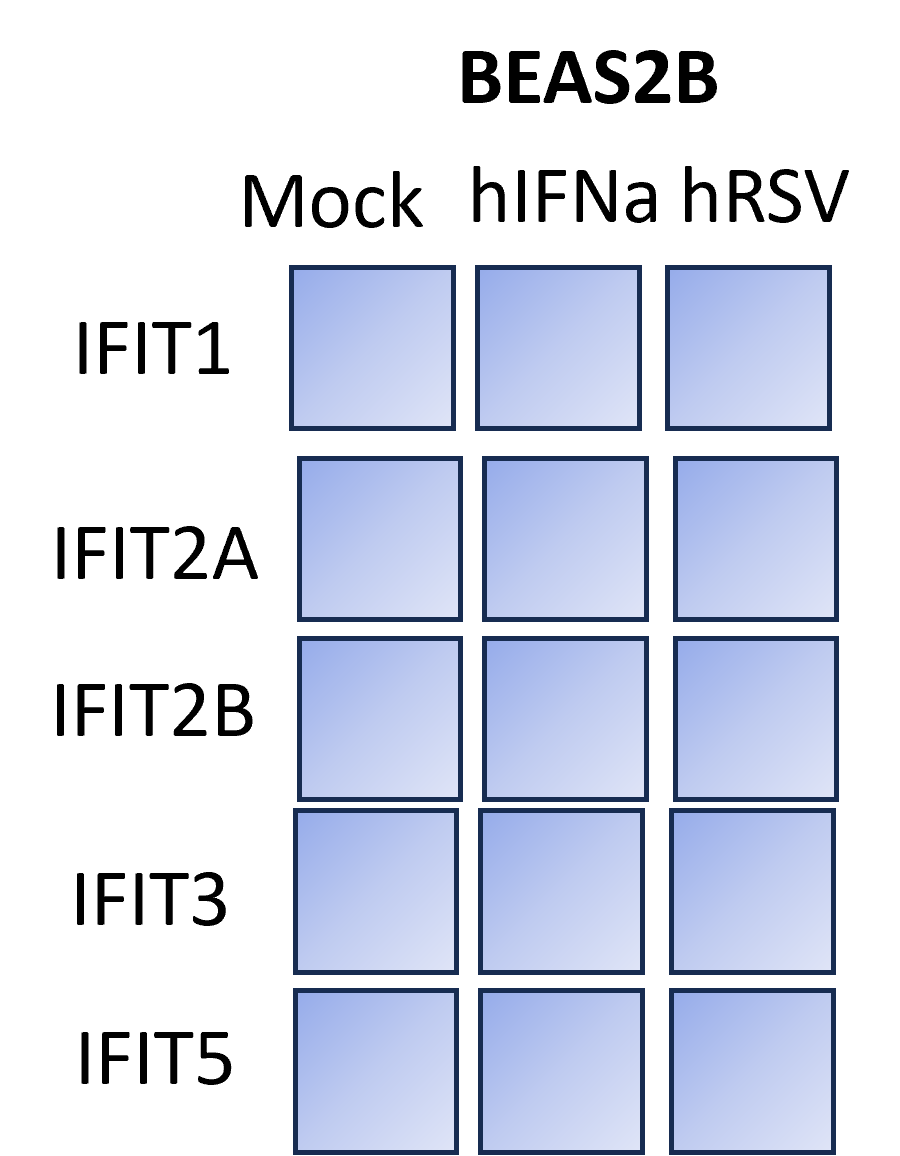
\includegraphics[width=1\linewidth]{06. Chapter 1/Figs/02. Localisation/03. beas2b merges.png}
    \caption[BEAS-2B localisation mergers.]{BEAS-2B localisation mergers.}
    \label{BEAS-2B localisation mergers.}
\end{figure}


\begin{figure}
    \centering
    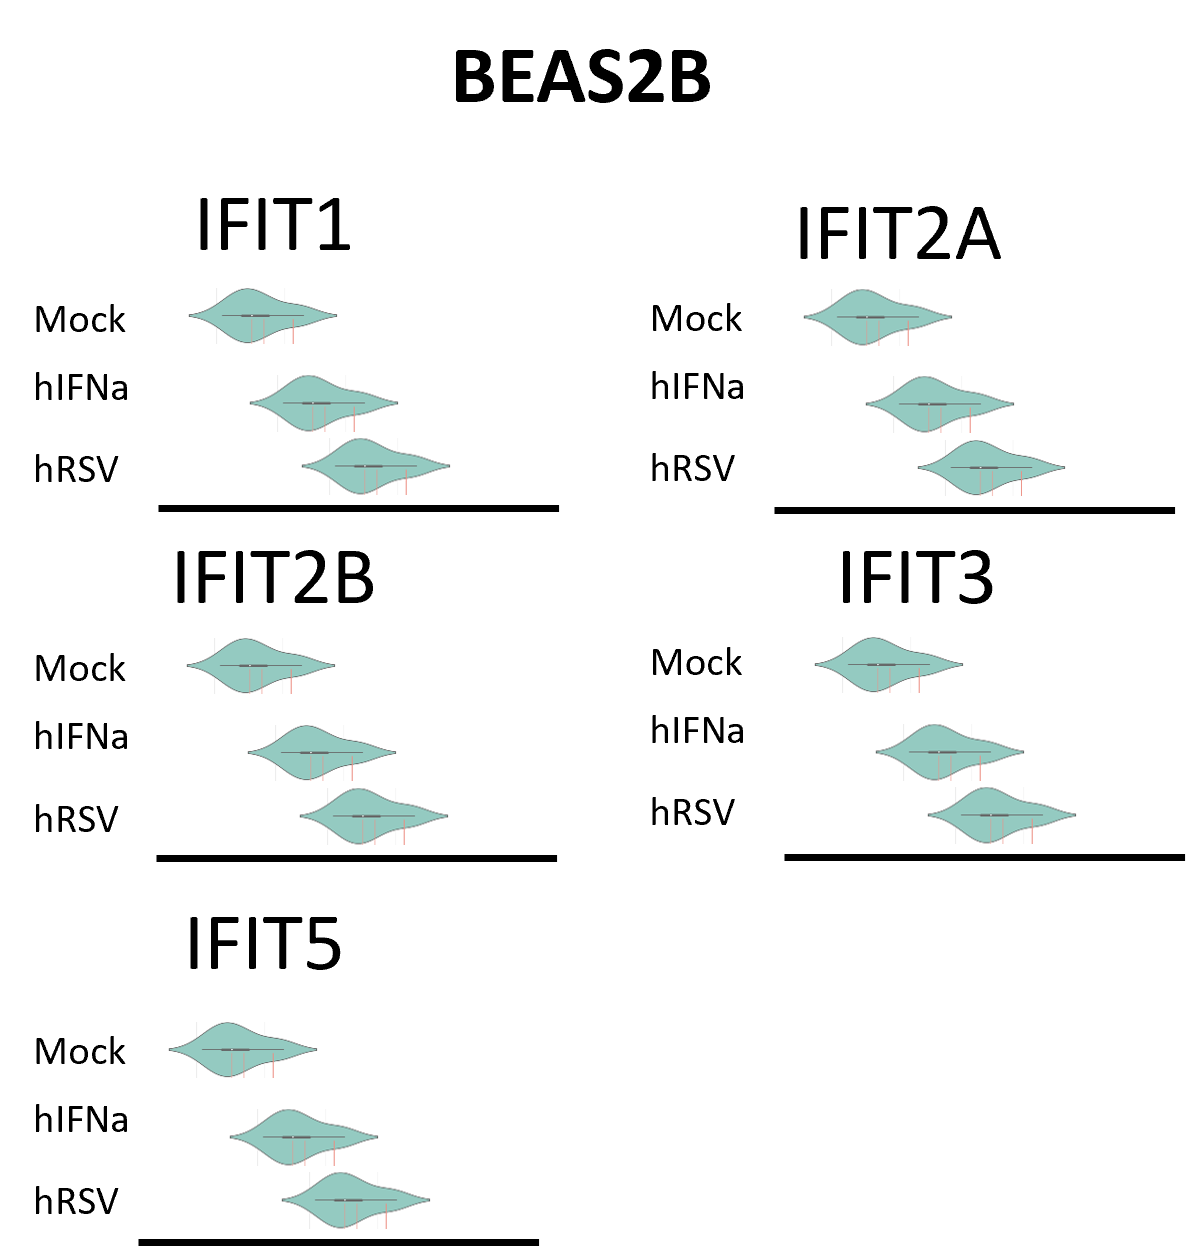
\includegraphics[width=1\linewidth]{06. Chapter 1/Figs/02. Localisation/04. beas2b plots.png}
    \caption[BEAS-2B localisation plots.]{BEAS-2B localisation plots.}
    \label{BEAS-2B localisation plots.}
\end{figure}





\section{Discussion} \label{Discussion-Chapter 1}
Recap human induction \newline
Recap human localisation



\nomenclature[z-IU]{IU}{International Units}
\nomenclature[z-PS]{PS}{Primer Set}
\nomenclature[z-MOI]{MOI}{Multiplicity of Infection}
\nomenclature[z-HPI]{HPI}{Hours Post Infection}
\chapter{Assessment of Transcriptional Induction of Bovine IFITs in the Context of RSV} \label{ch:Assessment of Transcriptional Induction of Bovine IFITs in the Context of RSV}
\section{Background and Aims} \label{sec:Background and Aims Chapter2}
From published literature, it is evident that induced human \textit{IFIT} expression negatively impacts RSV replication. The results obtained in Chapter \ref{ch:Assessment of Transcriptional Induction of Human IFITs in the Context of RSV} confirm the differential expression of human \textit{IFITs} in response to both hRSV and bRSV infections. However, an investigation into \textit{in vitro} bovine \textit{IFIT} induction and its potential influence on bovine RSV has not been undertaken to date.

Our hypothesis posited that bovine \textit{IFITs} would be induced by both human and bovine RSV, similar to the observations made for human \textit{IFITs} in the previous chapter. Our objective was to systematically test this hypothesis, employing methodologies akin to those used in Chapter \ref{ch:Assessment of Transcriptional Induction of Human IFITs in the Context of RSV}. Initially, our efforts were directed towards preparing essential technological materials and information, such as qPCR primers for \textit{bIFIT} detection. Additionally, we aimed to assess bRSV growth in various model bovine cell lines employed in our study. Subsequently, we sought to confirm the capability of our model cell lines to induce \textit{IFITs} following the treatment with known activators of the innate immune system, such as IFN$\upalpha$ and LPS. Following this, our strategy involved evaluating \textit{IFIT} induction during both human and bovine RSV infections, utilising a range of viral concentrations and various end assay time points.

\section{Results} \label{sec:Results Chapter2}
\subsection{Technology Establishment} \label{subsec:Technology Establishment}
\subsubsection{Primer Design and Validation for Bovine \textit{IFIT} Quantification} \label{Primer Design and Validation for Bovine IFIT Quantification}
We devised a panel of three qPCR primer sets (PS) for each bovine \textit{IFIT} gene. Detailed information about this process is outlined in Section \ref{subsec:Primer Design and Assay Setup}. Briefly, we inputted the coding sequences into the PrimerQuest software (Integrated DNA Technologies) to identify the most suitable oligonucleotides. To evaluate the amplification efficiencies of each primer set, we employed serial dilutions of \textit{IFIT} DNA clones from a bovine ISG library as standards (accessible through a collaboration with CVR Glasgow). The outcomes are depicted in Figure \ref{fig:Validation of custom-made bIFIT qPCR primers}. The graph demonstrates that primer sets 1 exhibited the most favourable amplification efficiencies. All primer sets, except for \textit{bIFIT3}, yielded amplification efficiencies of around 100\%. Consequently, they were chosen for subsequent experiments. While \textit{bIFIT3} primer sets demonstrated similar outcomes in terms of standard curve slopes and amplification efficiencies, PS1 consistently outperformed the others in repeated testing rounds (data not presented). As a result, it was selected for further experimentation.

\begin{figure}
    \centering
    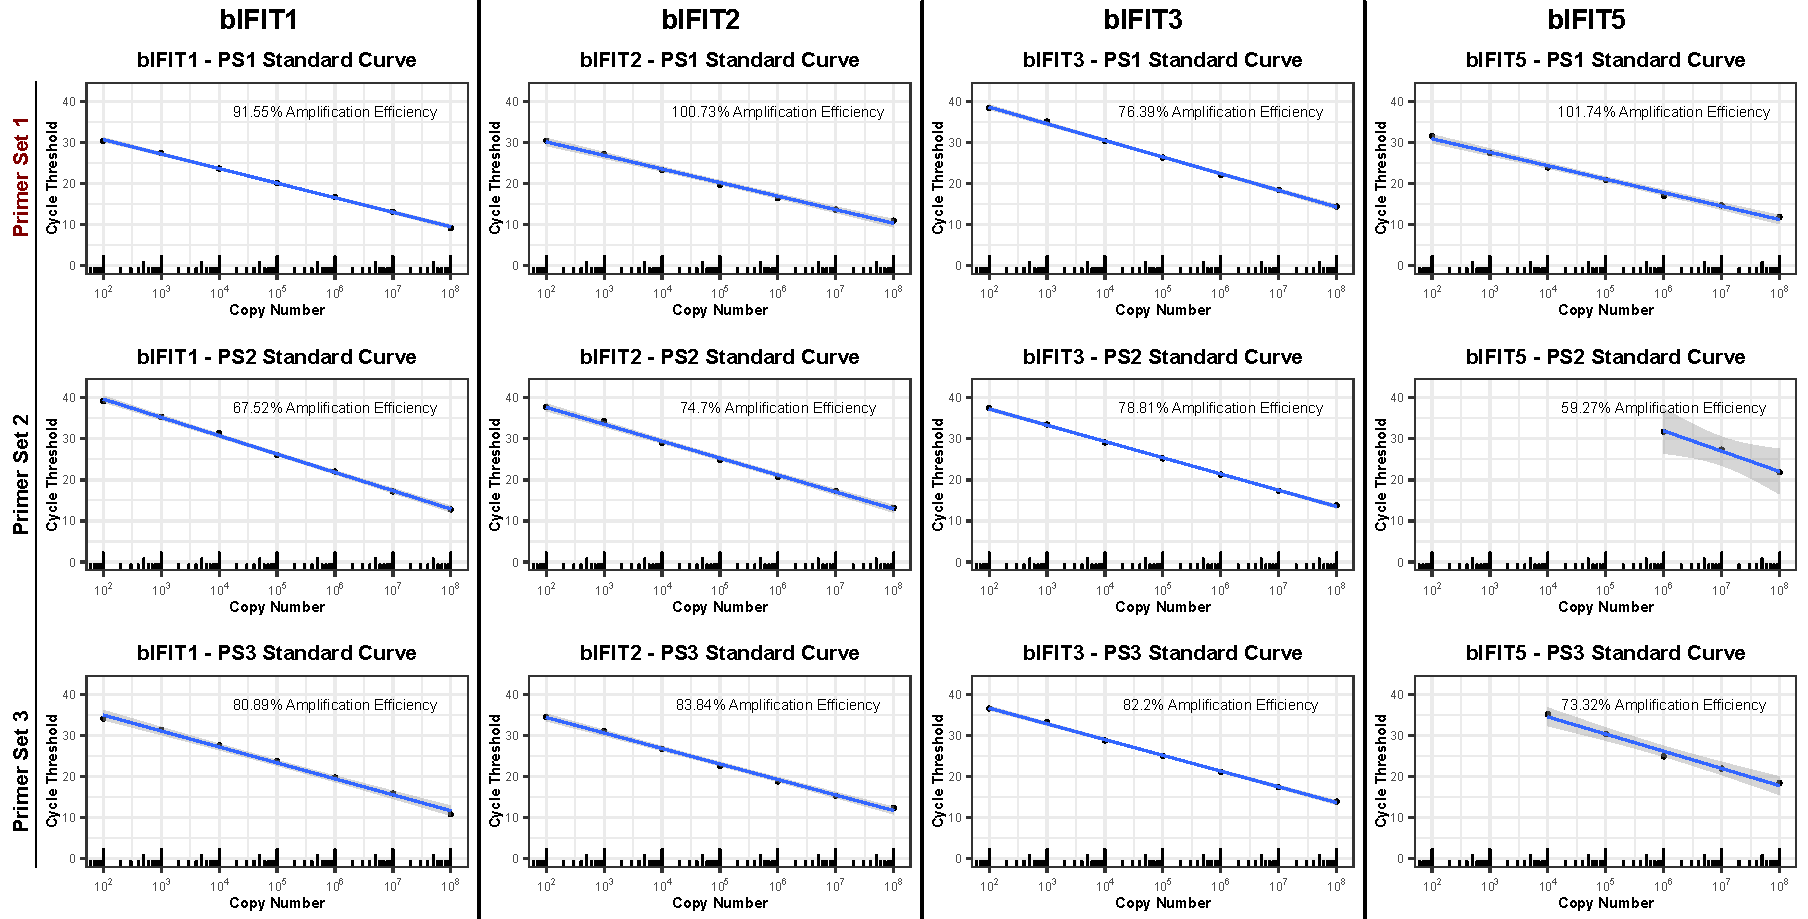
\includegraphics[width=1\linewidth]{07. Chapter 2/Figs/01. Technologies/02. primer validation.pdf}
    \caption[Validation of Custom-Made \textit{bIFIT} qPCR Primers.]{\textbf{Validation of Custom-Made \textit{bIFIT} qPCR Primers.} The custom-designed primers were evaluated by creating a serial dilution of bovine \textit{IFIT}-containing plasmids, provided by the CVR Glasgow. The resulting standard curves are shown here. Primer set (PS) 1, 2, and 3 are depicted for bovine \textit{IFIT1}, \textit{IFIT2}, \textit{IFIT3}, and \textit{IFIT5}, along with their calculated amplification efficiencies. Primer sets 1 (highlighted in red) were selected for further downstream analyses.}
    \label{fig:Validation of custom-made bIFIT qPCR primers}
\end{figure}

The PSs behaviour was monitored throughout the project, as fresh standard curves were created per experiment. Figure \ref{fig:The Performance of Custom Made Primer Sets Over Time} shows that the average data is consistent with what was observed in initial testing (Figure \ref{fig:Validation of custom-made bIFIT qPCR primers}), however, there were per experiment deviations in slope angles for each of the selected primer pairs. The underlying amplification efficiencies stayed consistent, as is highlighted by the averaged efficiencies displayed. The initial \textit{bIFIT3} PSs amplification slopes were different compared to the other \textit{bIFIT} PSs. They as well presented a more variable nature of its amplification efficiencies throughout the project. This prohibited the usage of $\Updelta$$\Updelta$Ct methodologies for transcript quantification as the increase in cycle threshold would not be proportional to the decrease of transcript abundance between the \textit{bIFITs}, and thus a different methodology had to be adopted. This is described in detail in Section \ref{subsec:Data Processing}. In short, the copy numbers were deducted from standard curves and factorised by the relative abundance of bovine \textit{GAPDH}. This ensured the slope-independent establishment of relative expression values, mirroring and complementing data from $\Updelta$$\Updelta$Ct methodologies.

\begin{figure}
    \centering
    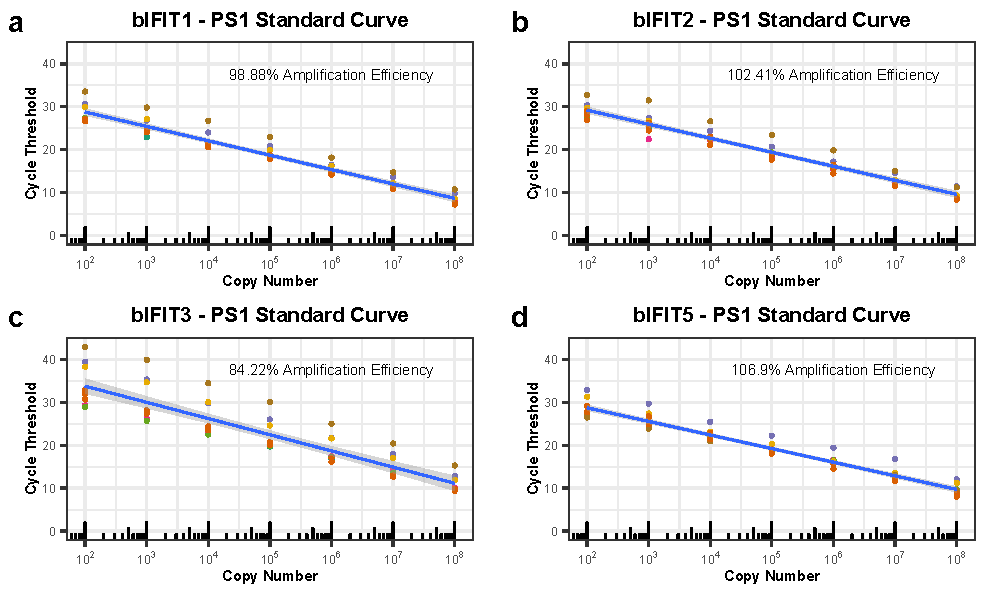
\includegraphics[width=1\linewidth]{07. Chapter 2/Figs/01. Technologies/03. standard curves behaviour.pdf}
    \caption[The Performance of Custom-Made Primer-Sets Over Time.]{\textbf{The Performance of Custom-Made Primer-Sets Over Time.} Fresh standard curves were prepared during experiments with custom-made \textit{bIFIT} qPCR primers. The figure illustrates the average amplification efficiencies and standard curves compiled across all experiments, with individual experiments represented by distinct colors.}
    \label{fig:The Performance of Custom Made Primer Sets Over Time}
\end{figure}

\subsubsection{Growth Curves of Bovine RSV in Bovine Cell Lines} \label{Growth Curves of Bovine RSV in Bovine Cell Lines}
Although my colleagues in the Viral Glycoproteins Group from the Pirbright Institute routinely perform hRSV infections of the MDBK cell line, data in the BT cell line is currently lacking. Therefore we set up bRSV growth curves in both cell lines side by side to investigate which time points would be relevant for further infection experiments. Crude-extracted bRSV, isolated as described in Section \ref{subsec:Virus Propagation and Production} and quantified as described in Section \ref{subsec:Virus Quantification by TCID50 Assay} was used for the establishment of growth curves as described in Section \ref{subsec:Viral Growth Curves}. In brief, the MDBK and the BT cell line were seeded in 96-well plates and infected with WT bRSV at MOI 0.1. The supernatant and cellular fractions were collected at time intervals of 24, 48, 72, 96, 120, 144, and 168 hours post-infection, snap frozen in a dry ice-ethanol bath, and later tittered as described in Section \ref{subsec:Virus Quantification by TCID50 Assay}. As can be observed in Figure \ref{fig:bRSV growth curves in MDBK and BT cell lines}, there is a differential infection profile between the cell lines. bRSV growth in the MDBK cell line was initially exponential, starting at \(10^{2.5}\) viral titre solely detected in the cytosolic fraction at 24 HPI, it increased to \(10^{4}\) and \(10^{3}\) for the cellular and supernatant fractions respectively at 48 hours. At 72 hours, the cellular viral titre reached \(10^{4.5}\), while the supernatant one further increased to \(10^{3.5}\). Afterwards, the cellular titre remained stable until 120 hours, after which it declined by more than an order of magnitude to \(10^{3}\) at 144 hours and then further increased again to \(10^{3.5}\) at 168 hours. The supernatant titre increased to \(10^{4.5}\) and \(10^{5.5}\) at 120 and 144 hours respectively, and afterwards it decreased to \(10^{4.5}\) again at 168 hours. The peak combined titre occurred at 144 hours but it was robust from 48 hours onwards. bRSV growth in BT cell line displayed virtually no titre from supernatant fraction at 24 and 48 hours. Regardless, the 24-hour time point was the peak value of the combined, as well as cellular titre with intracellular titres of \(10^{4}\) at 24 hours and \(10^{3}\) at 48 hours. Intracellular titres further declined to \(10^{2}\) at 72 hours, and since then they remained stable other than a small increase to \(10^{2.5}\) at 120 HPI. On the other hand, supernatant titre peaked at 72 hours at \(10^{4}\), slightly decreased to \(10^{3.5}\) at 120 hours and afterwards stayed stable until the end of the experiment. From this experiment, we can conclude that the viral replication kinetics differ substantially between the two cell lines and the data suggests that we can be certain of viral replication at 48 HPI in the MDBK cell line and 24 HPI in the BT cell line.

\begin{figure}
    \centering
    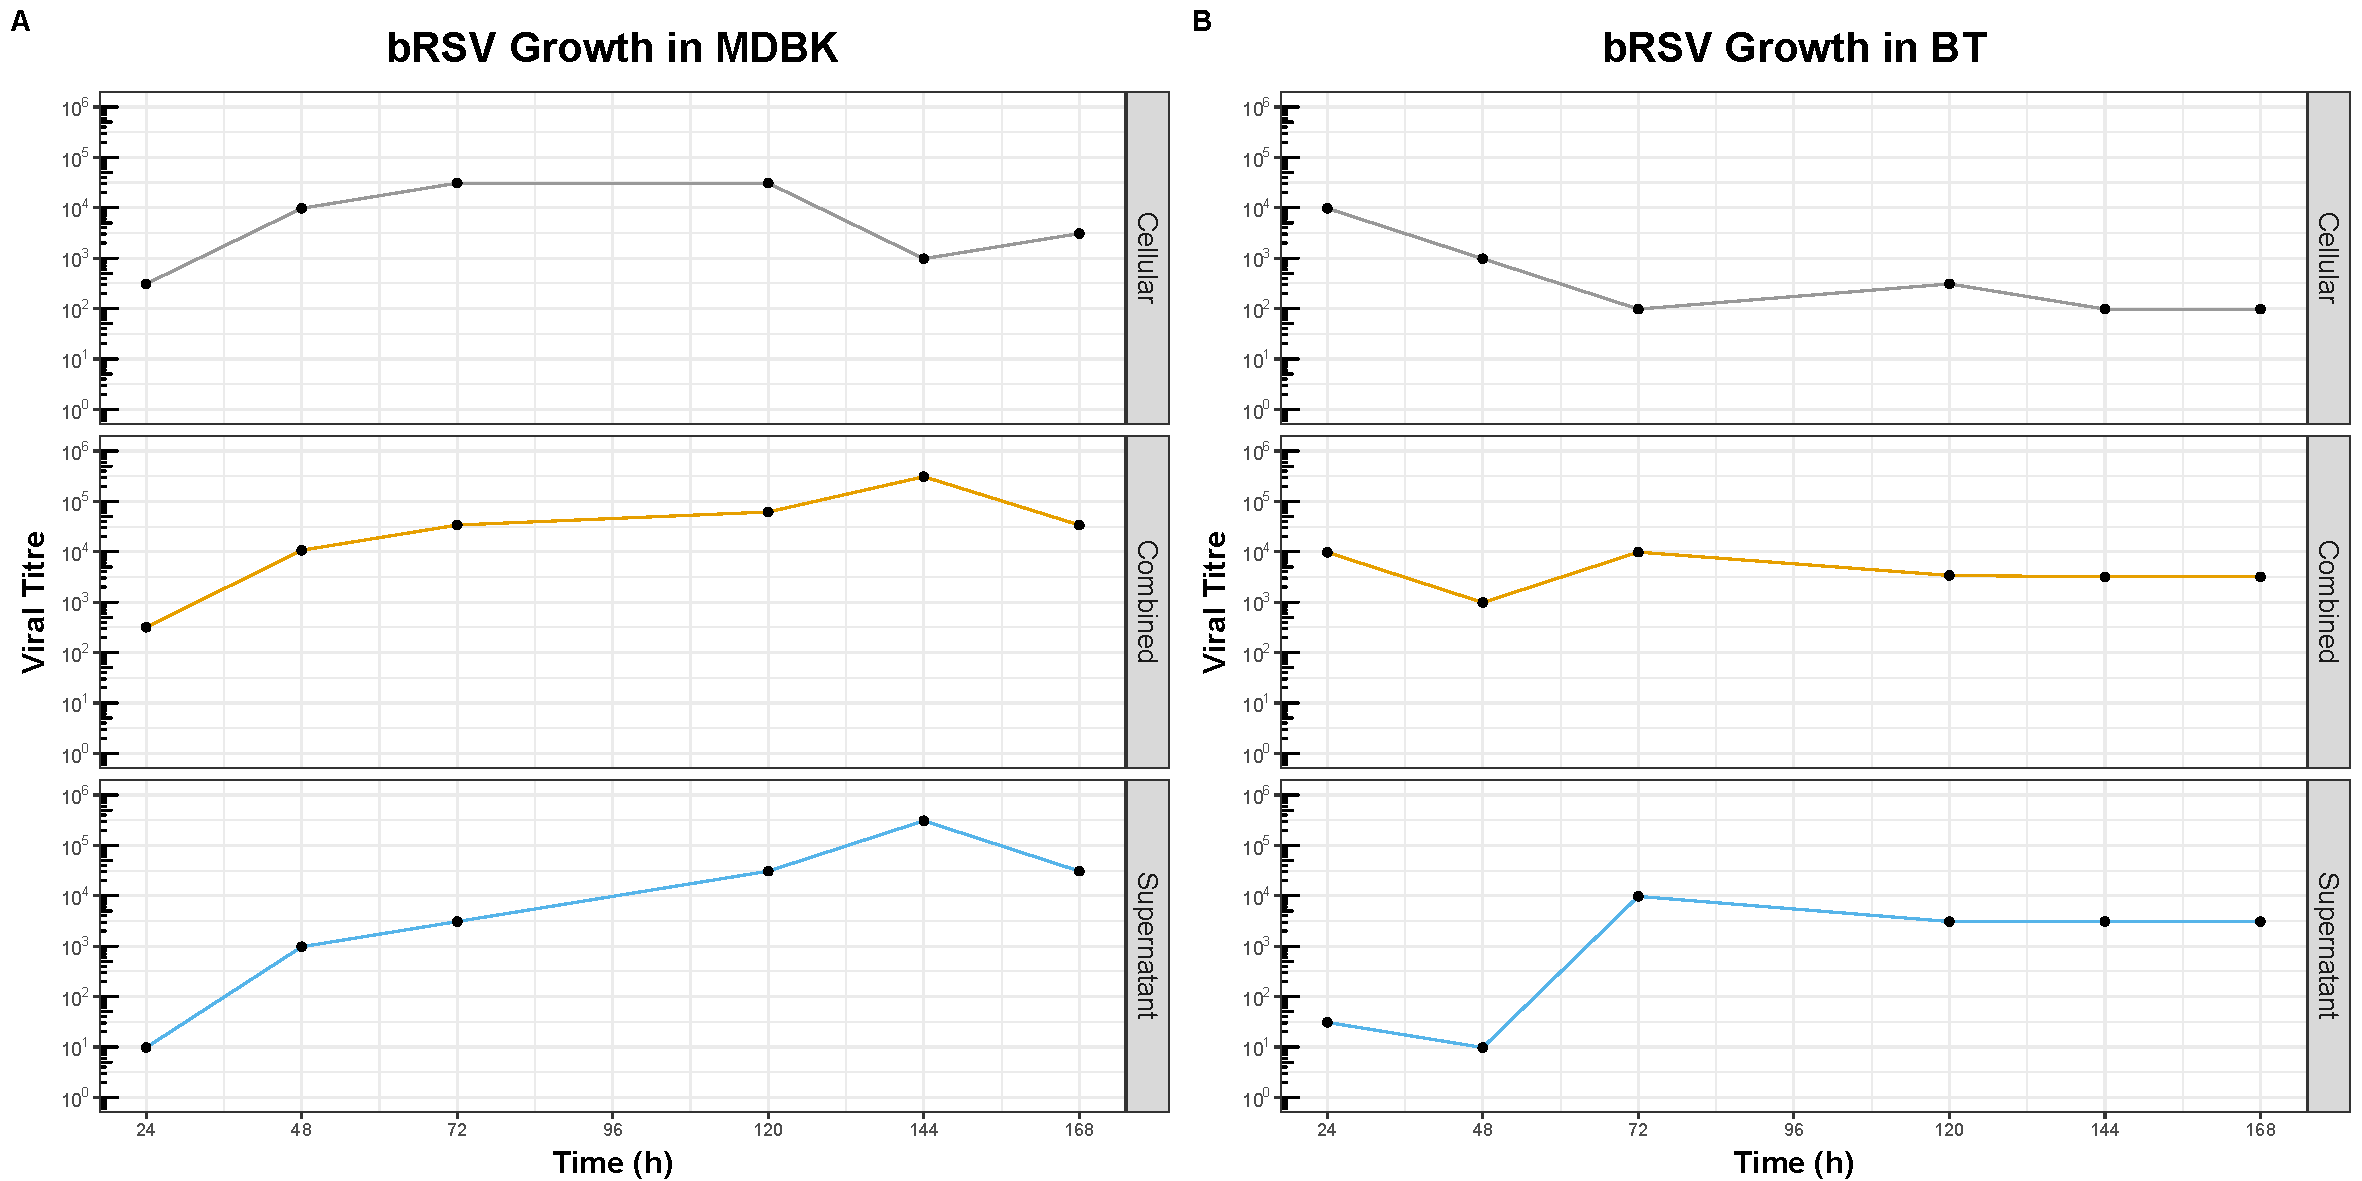
\includegraphics[width=1\linewidth]{07. Chapter 2/Figs/01. Technologies/01. growth_curves.pdf}
    \caption[bRSV Growth Curves in MDBK and BT Cell Lines.]{\textbf{bRSV Growth Curves in MDBK and BT Cell Lines.} MDBK and BT cell lines were infected with 0.1 MOI wild-type bRSV and the cellular (top panel) and supernatant (bottom panel) fractions were extracted at time intervals of 24, 48, 72, 96, 120, 144, and 168 hours post-infection. These were subsequently quantified by TCID50 methodology. The total viral titre is shown in the middle panel.}
    \label{fig:bRSV growth curves in MDBK and BT cell lines}
\end{figure}

Having established and validated the tools for the quantification of bovine \textit{IFITs} and elucidated the optimal assay termination time points for bRSV infections, we were equipped to replicate the analysis conducted in Chapter \ref{ch:Assessment of Transcriptional Induction of Human IFITs in the Context of RSV}. Our goal was to systematically assess the induction of \textit{bIFITs}, starting with different activators of the innate immune system, followed by bRSV infection, and finally, evaluating cross-species defense against hRSV infection. The relative induction levels were assessed using RT-qPCR methodology, as described in Section \ref{sec:Quantitative Real Time/Reverse Transcription PCR}. Briefly, cells were cultured in 12-well plates and exposed to the respective stimulants. At the endpoint of the experiments, RNA extraction was performed, followed by complementary DNA (cDNA) synthesis and transcript quantification through qPCR. The expression of \textit{hRSV N}, \textit{bRSV N}, and \textit{bMx1} genes was quantified using the \(\Delta\)\(\Delta\)Ct method, standardized to the bovine \textit{GAPDH} gene, and further normalized against mock-treated samples. As described previously, bovine \textit{IFIT} genes copy numbers were extrapolated from standard curves, created freshly per experiment, normalized relative to the mock copy numbers, and further standardized to the relative levels of bovine \textit{GAPDH} detected per experimental condition. The statistical analysis adhered to the procedures outlined in Section \ref{sec:Statistical Analysis}. It's important to note that the selection of the appropriate statistical test was contingent upon the assessment of data distribution normality and equality of variance, considerations that will be elaborated upon in the subsequent sections of this chapter.

\subsection{Bovine \textit{IFIT} Responses to Activators of Innate Immune Response} \label{subsec:Bovine IFIT Responses to Activators of Innate Immune Response}
The Madin-Darby bovine kidney (MDBK) cell line, derived from bovine renal epithelium in 1958 (\cite{Madin1958EstablishedOrigin}), serves as a well-established model system in bovine virology studies. We assessed the cells for the induction potential of bovine \textit{IFITs} along with bovine \textit{Mx1} using bovine IFN\(\alpha\) and LPS (bovine IFN\(\gamma\) was not commercially available). Bovine \textit{Mx1} was included in the analyses due to its status as an Interferon-Stimulated Gene (ISG), widely reported in immunology and virology studies, and as we observed minimal bovine \textit{IFIT} responses throughout the study, to ensure the cell lines had functioning internal pathways for ISG induction. Figure \ref{fig:MDBK responses to bIFNa} displays the \textit{bIFIT} and \textit{bMx1} responses to stimulation with bIFN\(\alpha\) at a concentration of 5 ng/mL (equivalent to 1,000 UI/mL of hIFN\(\alpha\)) for either 3 or 6 hours.

The data reveals that all assayed genes were significantly upregulated biologically within 3 hours of induction, although the magnitude varied substantially. For the bovine \textit{IFITs}, all exhibited higher induction at 3 hours compared to 6 hours. The \textit{bIFITs} displayed a similar induction pattern to that observed in A549 cells, with \textit{bIFIT1} showing the strongest response, \textit{bIFIT2} and \textit{bIFIT3} displaying medium responses of similar amplitudes, and \textit{bIFIT5} exhibiting the lowest response. Notably, \textit{bIFIT1} showed the highest induction at 20-fold and 5-fold for 3 and 6 hours of incubation, respectively, and was the only bovine \textit{IFIT} that exhibited biologically significant induction at 6 hours. \textit{bIFIT2} and \textit{bIFIT3} were induced by 6-fold and 3.5-fold for 3 and 6-hour incubations with bIFN\(\alpha\) respectively, while \textit{bIFIT5} was induced by 4-fold and 2-fold for the same respective periods. Regarding \textit{bMx1}, its response surpassed that of the bovine \textit{IFITs}, showcasing a time-dependent induction increasing from 32-fold to 120-fold as the treatment continued. This shows that MDBK cells are capable of \textit{bIFIT} and \textit{bMx1} induction, albeit with differing temporal dynamics. However, these responses are modest, especially compared to the previously observed human \textit{IFIT} responses to IFN\(\alpha\). As a side note, while the datasets for \textit{bIFIT3} and \textit{bIFIT5} exhibited a normal distribution of data with equal variances, datasets for \textit{bIFIT1}, \textit{bIFIT2}, and \textit{bMx1} exhibited normal distributions with unequal variances.

\begin{figure}
    \centering
    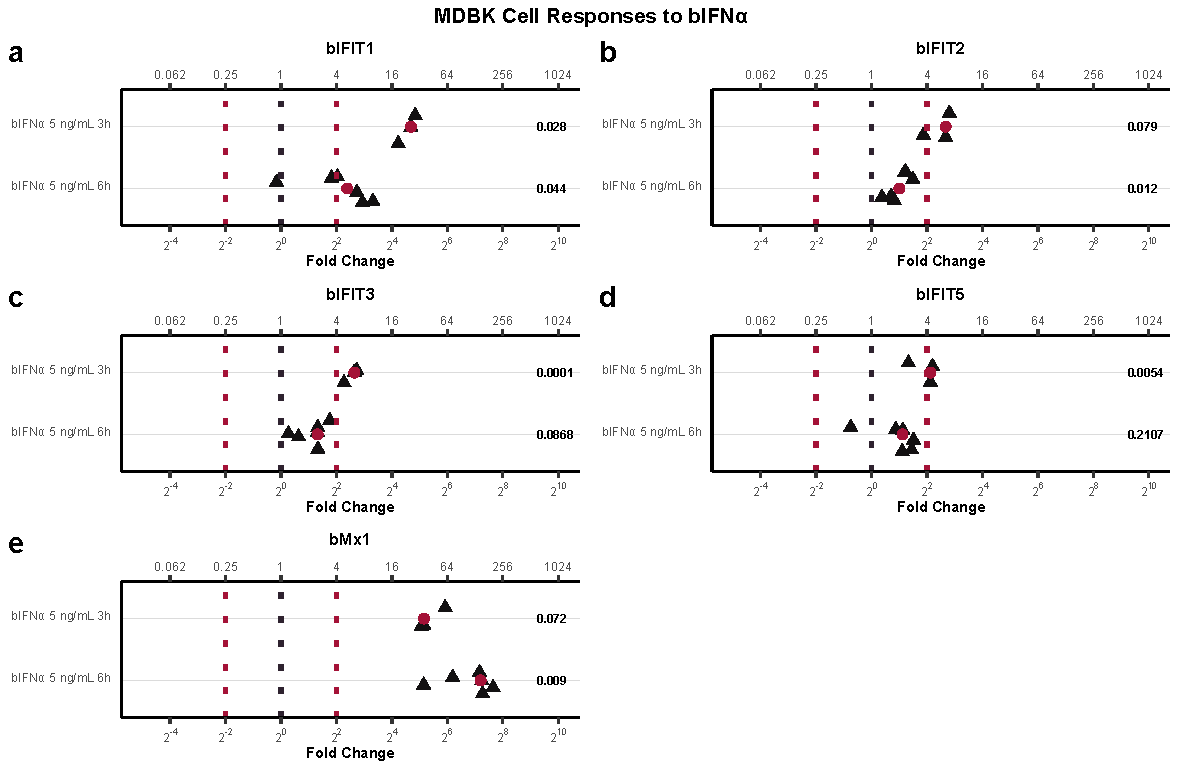
\includegraphics[width=1\linewidth]{07. Chapter 2/Figs/02. Induction/01. mdbk_treat_bifna.pdf}
    \caption[\textit{bIFIT} Gene Expression in MDBK Cells in Response to bIFN\(\alpha\) Stimulation.]{\textbf{\textit{bIFIT} Gene Expression in MDBK Cells in Response to bIFN\(\alpha\) Stimulation.} (a) \textit{bIFIT1}, (b) \textit{bIFIT2}, (c) \textit{bIFIT3}, (d) \textit{bIFIT5}, and (e) \textit{bMx1} gene expression levels were assessed using quantitative real-time PCR (qPCR) in MDBK cells following stimulation with bovine interferon alpha (IFN\(\alpha\)) at a concentration of 5 ng/mL for a treatment duration of either 3 or 6 hours. Relative expression values are normalized to standardized mock-treated samples. Median values are represented by red circles. The black dotted line represents mock expression levels, while the red dotted lines indicate biologically significant induction thresholds. Numeric values indicate the p-values compared to mock-treated samples.}
    \label{fig:MDBK responses to bIFNa}
\end{figure}

Furthermore, we aimed to investigate the involvement of Toll-like Receptor 4 (TLR4) in \textit{bIFIT} induction, previously observed to play a role in the A549 cell line (refer to Figure \ref{fig:A549 Response to LPS} in Section \ref{subsec:Human IFIT Responses to Activators of Innate Immune Response}). MDBK cells were incubated with LPS for 6 hours at concentrations of 0.5, 1, 2.5, 5, and 10 ng/mL. Subsequently, the cells were lysed, and their RNA was extracted, converted to cDNA, and quantified by qPCR as previously described. Our findings indicate that neither \textit{bMx1} nor \textit{bIFITs} were induced to biologically significant levels by LPS within the tested concentration range. Most time points revealed no relative change, while 2.5 ng/mL resulted in a 50\% reduction in the levels of \textit{bIFIT1}, \textit{bIFIT2}, and \textit{bIFIT3}. Evidently, the data suggests that LPS, at the tested concentrations, does not induce \textit{bMx1} or \textit{bIFITs}; if anything, it causes a slight downregulation of their expression. As a side note, while the datasets for \textit{bIFIT3}, \textit{bIFIT5}, and \textit{bMx1} exhibited a normal distribution of data with equal variances, the datasets for \textit{bIFIT1} and \textit{bIFIT2} showed normal distributions with unequal variances.


\begin{figure}
    \centering
    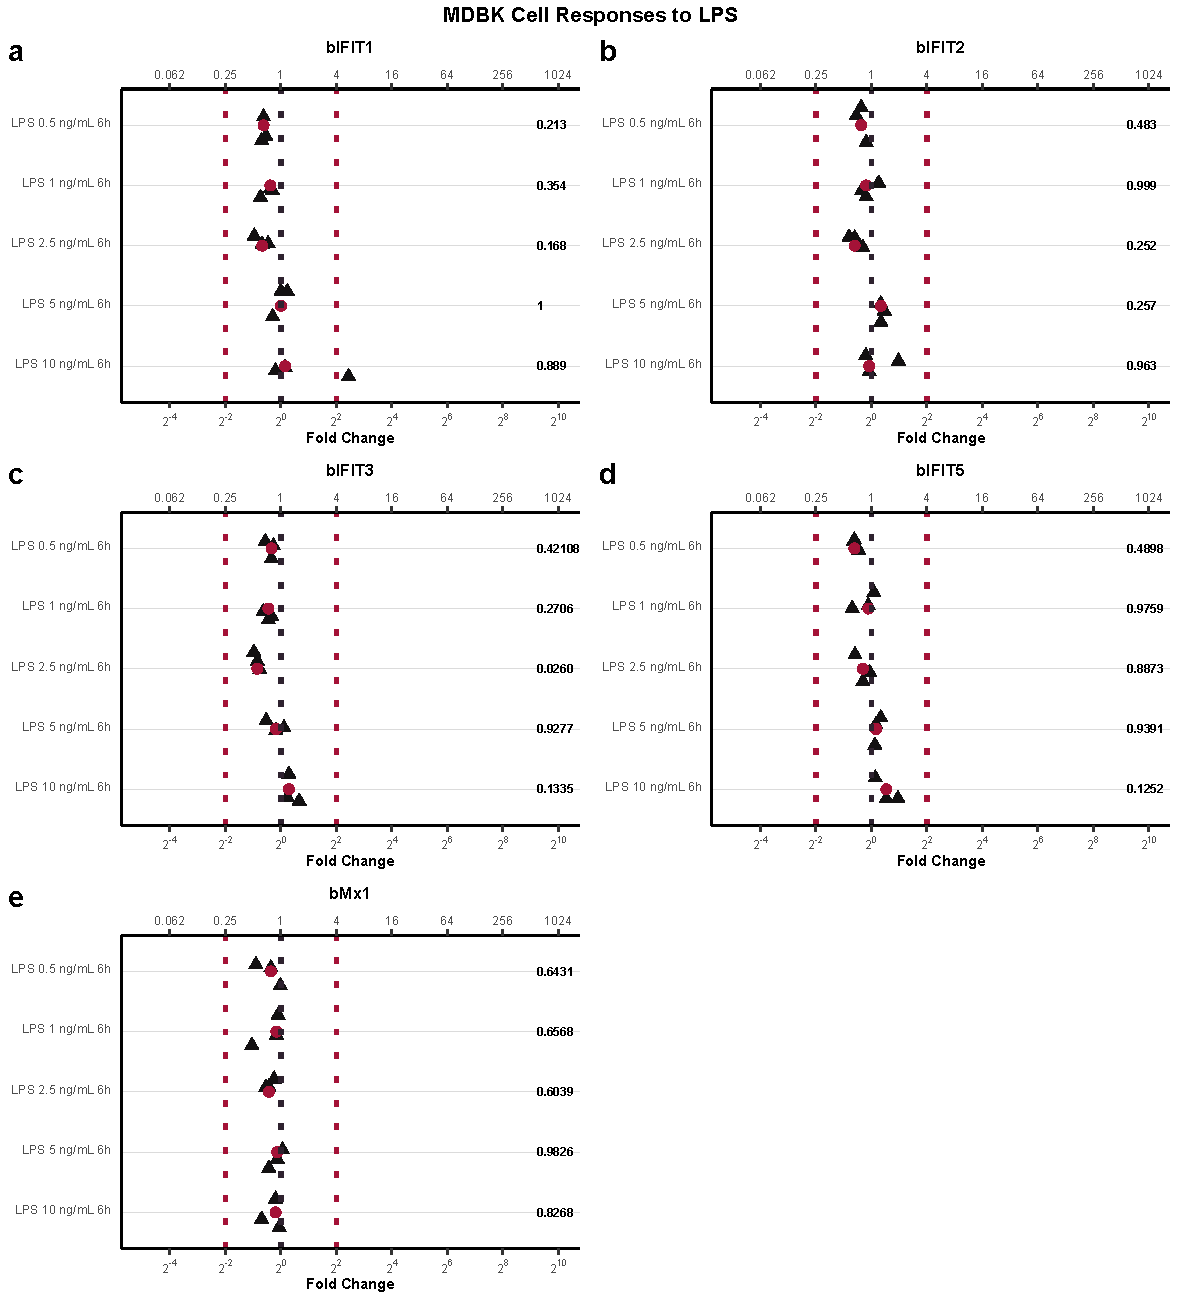
\includegraphics[width=1\linewidth]{07. Chapter 2/Figs/02. Induction/02. mdbk_treat_lps.pdf}
    \caption[\textit{bIFIT} Gene Expression in MDBK Cells in Response to LPS Stimulation.]{\textbf{\textit{bIFIT} Gene Expression in MDBK Cells in Response to LPS Stimulation.} (a) \textit{bIFIT1}, (b) \textit{bIFIT2}, (c) \textit{bIFIT3}, (d) \textit{bIFIT5}, and (e) \textit{bMx1} gene expression levels were assessed using quantitative real-time PCR (qPCR) in MDBK cells following stimulation with bacterial LPS at a concentration of 0.5, 1, 2.5, 5, and 10 ng/mL for a treatment duration of 6 hours. Relative expression values are normalized to standardized mock-treated samples. Median values are represented by red circles. The black dotted line represents mock expression levels, while the red dotted lines indicate biologically significant induction thresholds. Numeric values indicate the p-values compared to mock-treated samples.}
    \label{fig:MDBK responses to LPS}
\end{figure}

To validate the MDBK induction data, the BT cell line was employed. Originating from Bovine viral diarrhea virus (BVDV) negative bovine nasal turbinate cells, isolated in 1974 from a neonatal Holstein cow (\cite{McClurkin1974ComparisonVirus}), these cells, mentioned in Section \ref{Growth Curves of Bovine RSV in Bovine Cell Lines}, facilitate bRSV replication and originate from a more physiologically significant site in the bRSV life cycle compared to the MDBK cell line. BT cells were incubated with 5 ng/mL of bIFN\(\alpha\) for either 3 hours or 24 hours. Figure \ref{fig:BT responses to bifna} depicts the results. At 3 hours of treatment, all genes, except \textit{bIFIT2}, were induced to biologically significant levels. However, after 24 hours, the relative mRNA levels returned to basal levels. Specifically, \textit{bIFIT1} displayed the highest response with a 20-fold induction, followed by \textit{bMx1} with a 16-fold increase. \textit{bIFIT3} showed an 8-fold induction, while \textit{bIFIT5} exhibited a 4-fold increase. Notably, while the dataset for \textit{bIFIT2} displayed a normal distribution of data with equal variances, all other datasets showed normal distributions with unequal variances. In summary, it can be concluded that the BT cell line is sensitive to interferon and competent in \textit{bIFIT} induction. This data aligns with the MDBK data (Figure \ref{fig:MDBK responses to bIFNa}), revealing acute responses of \textit{bIFITs} to bIFN\(\alpha\) stimulation, although the induction is not sustained by 24 hours. Differences include the loss of induction persistence of \textit{bMx1} and the absence of bIFN\(\alpha\) sensitivity in \textit{bIFIT2}.

\begin{figure}
    \centering
    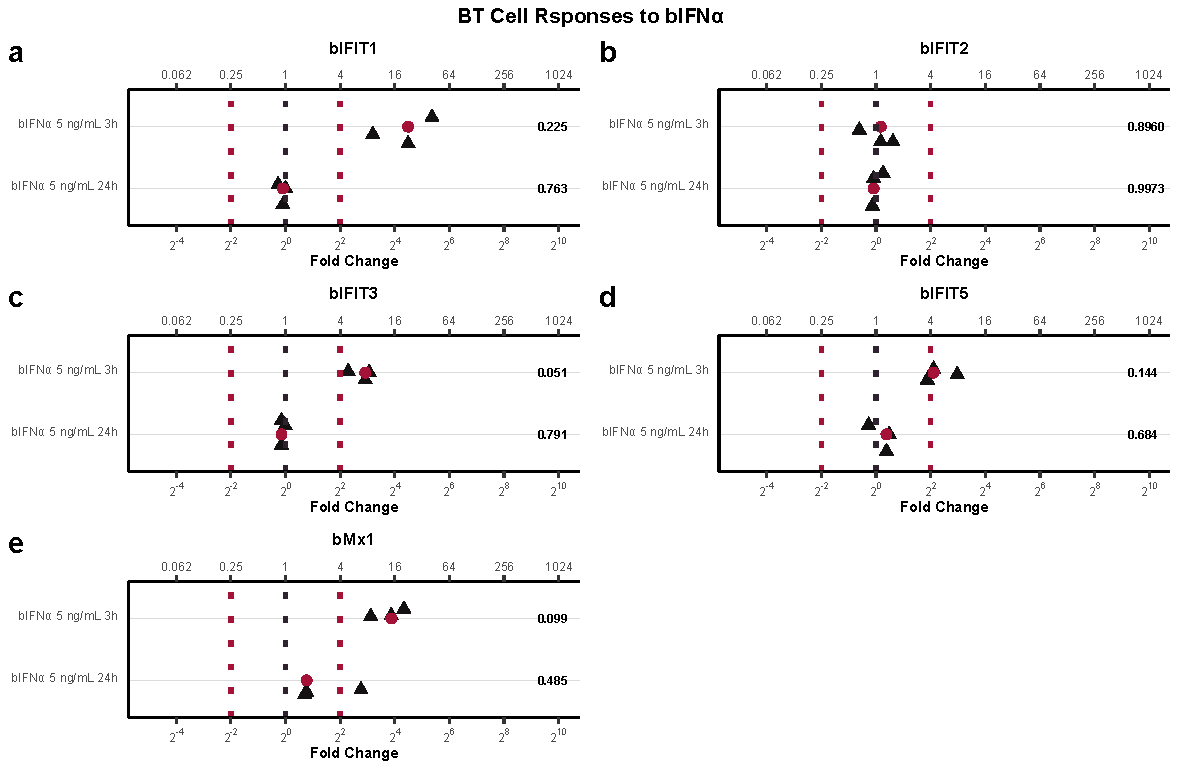
\includegraphics[width=1\linewidth]{07. Chapter 2/Figs/02. Induction/08. bt_bifna.pdf}
    \caption[\textit{bIFIT} Gene Expression in BT Cells in Response to bIFN\(\alpha\) Stimulation.]{\textbf{\textit{bIFIT} Gene Expression in BT Cells in Response to bIFN\(\alpha\) Stimulation.} (a) \textit{bIFIT1}, (b) \textit{bIFIT2}, (c) \textit{bIFIT3}, (d) \textit{bIFIT5}, and (e) \textit{bMx1} gene expression levels were assessed using quantitative real-time PCR (qPCR) in BT cells following stimulation with bovine interferon alpha (IFN\(\alpha\)) at a concentration of 5 ng/mL for a treatment duration of either 3 or 24 hours. Relative expression values are normalized to standardized mock-treated samples. Median values are represented by red circles. The black dotted line represents mock expression levels, while the red dotted lines indicate biologically significant induction thresholds. Numeric values indicate the p-values compared to mock-treated samples.}
    \label{fig:BT responses to bifna}
\end{figure}

\subsection{Bovine \textit{IFITs} Responses to Bovine RSV Infection} \label{subsec:Bovine IFITs Responses to Bovine RSV Infection}
Confirming the competence of the selected cell lines for \textit{bIFIT} induction, our goal was to evaluate the impact of bRSV infection on \textit{bIFIT} induction, particularly concerning varying viral MOIs and infection durations. To achieve this, MDBK cells were infected with crudely extracted bRSV at MOIs of 0.1, 1, and 2 for durations of 24 and 48 hours post-infection (HPI). The viruses employed in these experiments were prepared and quantified as detailed in Section \ref{subsec:Virus Propagation and Production} and Section \ref{subsec:Virus Quantification by TCID50 Assay}.

\begin{figure}
    \centering
    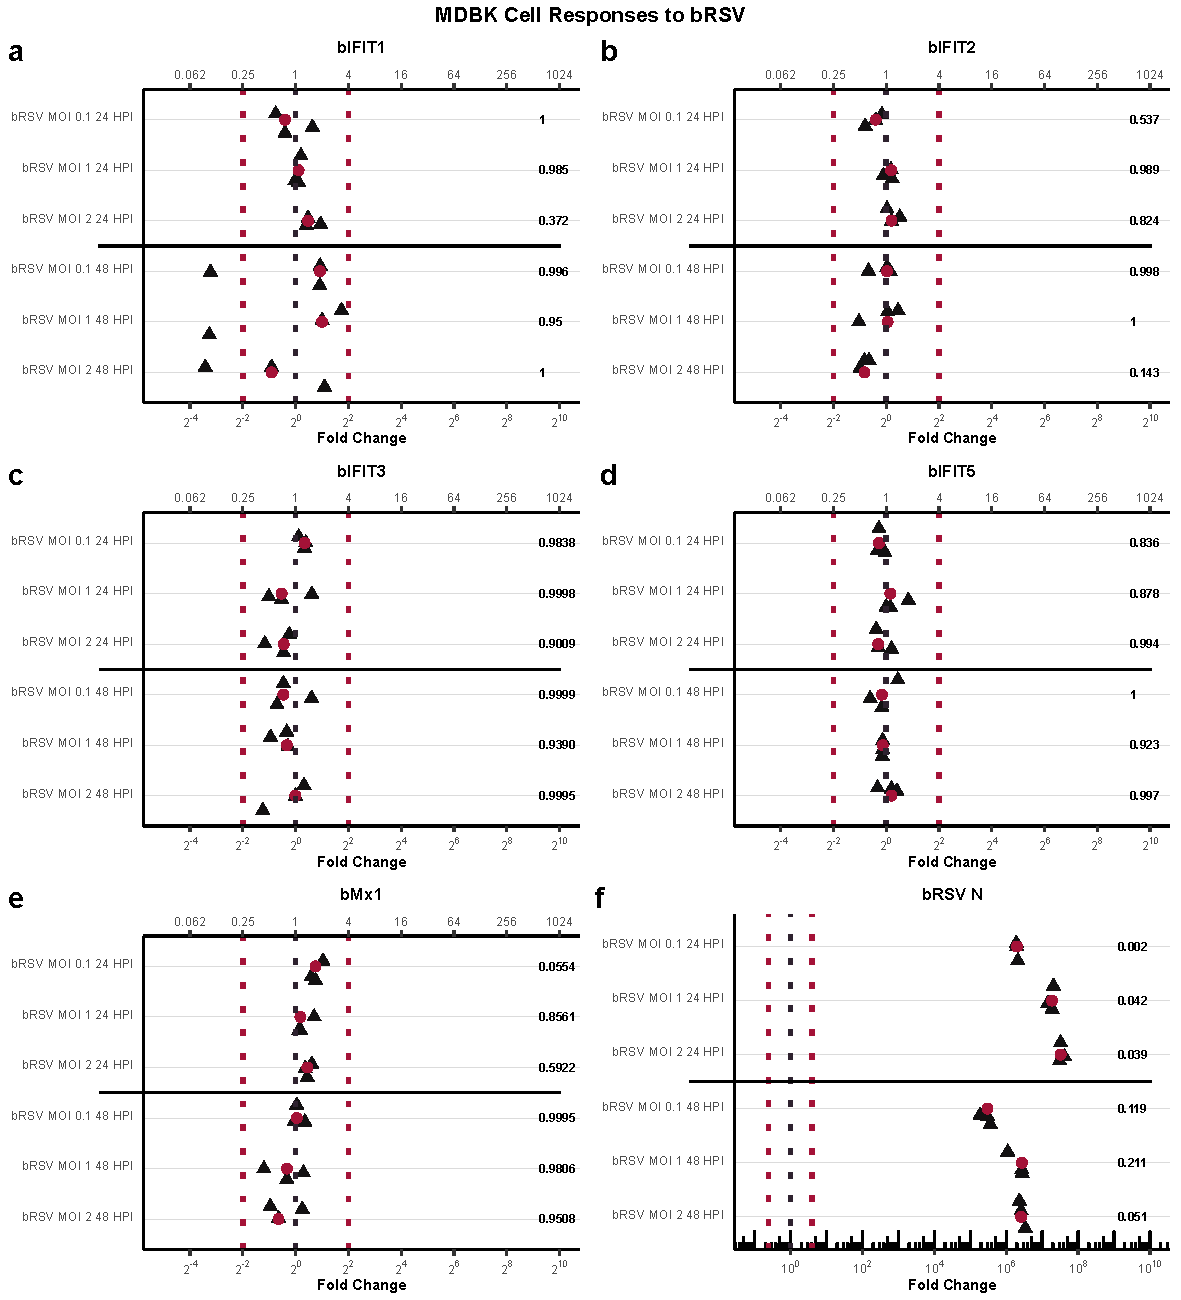
\includegraphics[width=1\linewidth]{07. Chapter 2/Figs/02. Induction/03. mdbk_brsv_timepoints.pdf}
    \caption[MDBK \textit{bIFIT} Response to bRSV Infection as a Function of Time and MOI.]{\textbf{MDBK \textit{bIFIT} Response to bRSV Infection as a Function of Time and MOI.} (a) \textit{bIFIT1}, (b) \textit{bIFIT2}, (c) \textit{bIFIT3}, (d) \textit{bIFIT5}, (e) \textit{bMx1} and (f) \textit{bRSV N} gene expression levels were assessed using quantitative real-time PCR (qPCR) in MDBK cell line following infection with bovine RSV at MOI of either 0.1, 1, or 2 for either 24 or 48 hours post-infection. Relative expression values are normalized to standardized mock-treated samples. Median values are represented by red circles. The black dotted line represents mock expression levels, while the red dotted lines indicate biologically significant induction thresholds. Numeric values indicate the p-values compared to mock-treated samples.}
    \label{fig:MDBK responses to bRSV timepoints}
\end{figure}

The results of this experiment are depicted in Figure \ref{fig:MDBK responses to bRSV timepoints}. Evidently, while bRSV demonstrated successful replication, as indicated by the notably high relative \textit{bRSV N} values across all tested MOIs and timepoints (panel f), there were no biologically significant alterations in the mRNA levels of either \textit{bMx1} or \textit{bIFITs}. Specifically, while the mRNA levels of \textit{bIFIT3} and \textit{bIFIT5} remained unchanged under all conditions, minor positive and negative changes were observed in the expression of the other genes. Notably, \textit{bIFIT1} levels doubled for infections at 0.1 and 1 MOI at 48 HPI but decreased by half at MOI 2 at 48 HPI. \textit{bIFIT2} mRNA levels showed no significant changes except for the 2 MOI infection at 48 HPI. Additionally, \textit{bMx1} exhibited a two-fold induction in the case of 0.1 MOI infection at 24 HPI and a 50\% downregulation after 2 MOI infection at 48 HPI. From a statistical standpoint, the datasets for \textit{bIFIT3} and \textit{bMx1} showcased normal distributions and equal variances, while the others exhibited normal distributions with unequal variances. The minimal responses to bRSV infection are intriguing, particularly considering our human data from Chapter \ref{ch:Assessment of Transcriptional Induction of Human IFITs in the Context of RSV}, which indicates that the \textit{hIFIT} responses are predominantly mediated by IFN\(\alpha\). Furthermore, as discussed in Section \ref{subsec:Bovine IFIT Responses to Activators of Innate Immune Response}, we are aware that \textit{bIFITs}, especially \textit{bMx1}, respond to bovine IFN\(\alpha\) stimulation. It is plausible that certain constituents within the bRSV or specific cytokines or chemokines in the crudely extracted bRSV preparations might impede the cascades necessary for \textit{bIFIT} induction.

\begin{figure}
    \centering
    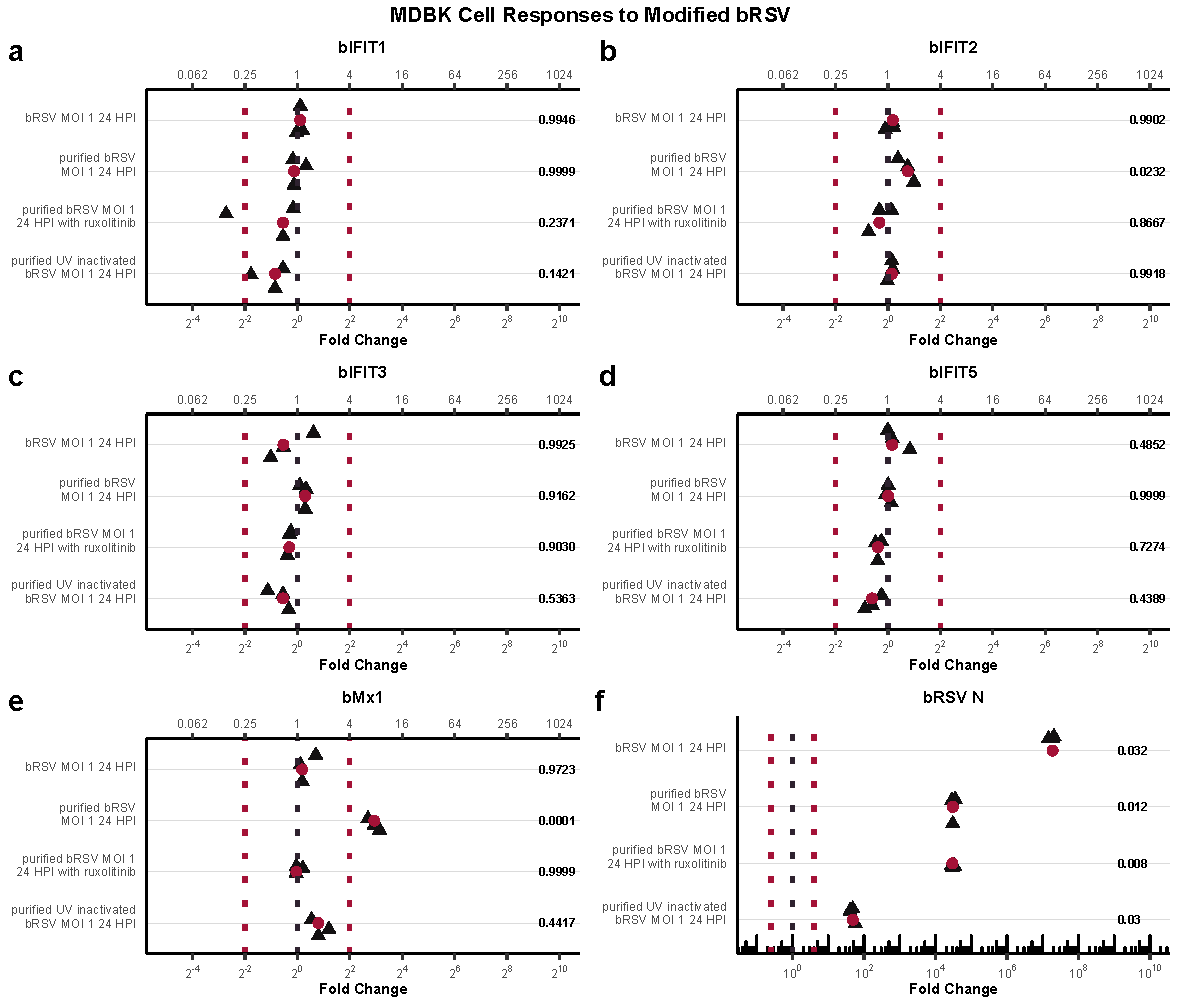
\includegraphics[width=1\linewidth]{07. Chapter 2/Figs/02. Induction/04. mdbk_brsv_uv_roxo.pdf}
    \caption[Impact of Ultra-Purification, UV-Inactivation, and INFR Inhibition on \textit{bIFIT} Induction in MDBK Cells Following bRSV Infection.]{\textbf{Impact of Ultra-Purification, UV-Inactivation, and INFR Inhibition on \textit{bIFIT} Induction in MDBK Cells Following bRSV Infection.} (a) \textit{bIFIT1}, (b) \textit{bIFIT2}, (c) \textit{bIFIT3}, (d) \textit{bIFIT5}, (e) \textit{bMx1}, and (f) \textit{bRSV N} gene expression levels were assessed using quantitative real-time PCR (qPCR) in MDBK cell line following infection with ultra-purified bRSV at MOI 1 for 24 hours. The cells were subjected to three different conditions: virus infection alone (top row), virus infection in the presence of 5 nM of ruxolitinib (interferon receptor inhibitor) throughout the infection (middle row), or UV-inactivated bRSV infection (bottom row). Relative expression values are normalized to standardized mock-treated samples. Median values are represented by red circles. The black dotted line represents mock expression levels, while the red dotted lines indicate biologically significant induction thresholds. Numeric values indicate the p-values compared to mock-treated samples.}
    \label{fig:The effect of ultra-purification, UV-inactivation and INFR inhibition on hIFIT induction following hRSV infection in MDBK}
\end{figure}

To investigate the possible influence of cellular contaminants on gene induction, MDBK cells were infected with ultrapurified bRSV, prepared through ultra-centrifugation on a discontinuous sucrose cushion as outlined in Section \ref{subsec:Virus Propagation and Production}. Simultaneously, we aimed to evaluate the impact of pharmacological inhibition of the interferon receptor and physical inactivation of bRSV on \textit{bIFIT} and \textit{bMx1} induction. This approach was prompted by our prior observation, as described in Section \ref{subsec:Human IFITs Responses to Human RSV} and illustrated in Figure \ref{fig:The effect of ultra-purification, UV-inactivation and INFR inhibition on hIFIT induction following hRSV infection in BEAS2B}, suggesting the requirement of basal interferon receptor activation for the maintenance of basal \textit{hIFIT} mRNA expression. The resultant data is displayed in Figure \ref{fig:The effect of ultra-purification, UV-inactivation and INFR inhibition on hIFIT induction following hRSV infection in MDBK}. Interestingly, the purification status of the virus did not influence the induction of \textit{bIFITs}. However, ultrapurification led to a seven-fold induction of \textit{bMx1}, a response that was entirely reversed by the presence of the interferon receptor inhibitor, ruxolitinib. Moreover, the presence of ruxolitinib marginally reduced the abundance of all \textit{bIFIT} mRNAs, though not to biologically significant levels. Intriguingly, the relative median \textit{bRSV N} mRNA value remained consistent between the first two conditions, contrary to our observations in human samples where the presence of ruxolitinib amplified the relative median \textit{bRSV N} mRNA. Additionally, UV-inactivation of bRSV resulted in only minor changes for all genes, approximately around \(\pm\)2 in magnitude. Overall, the induction response of \textit{bMx1} mirrors what was observed with human RSV in A549 and BEAS2B cell lines in Chapter \ref{ch:Assessment of Transcriptional Induction of Human IFITs in the Context of RSV}. Conversely, we did not observe any significant alterations in the mRNA levels of \textit{bIFITs}. This suggests that certain cellular contaminants present in crudely extracted bRSV preparations were suppressing the induction of \textit{bMx1}, whereas their absence had no bearing on the potential inhibition of \textit{bIFIT} induction. In terms of data distribution, while \textit{bRSV N} and \textit{bMx1} datasets exhibited normal distributions with unequal variances, the datasets for \textit{bIFIT1}, \textit{bIFIT2}, \textit{bIFIT3}, and \textit{bIFIT5} displayed normal distributions with equal variances.

\begin{figure}
    \centering
    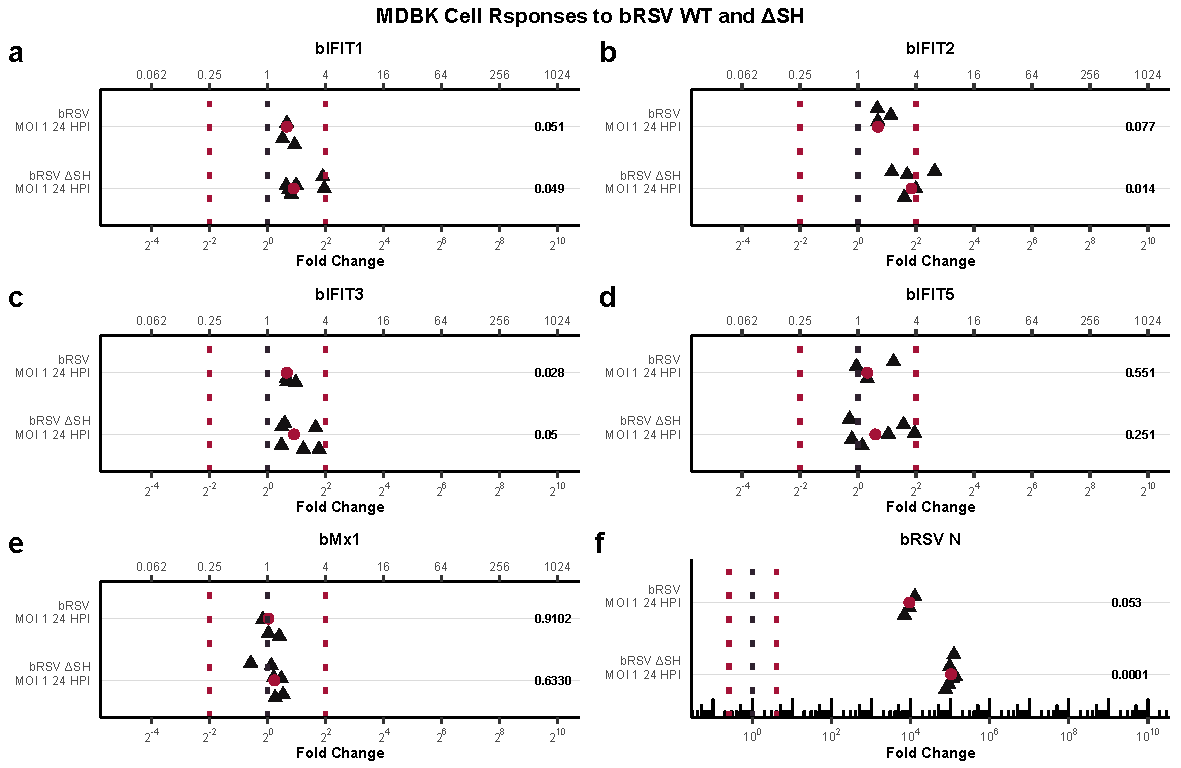
\includegraphics[width=1\linewidth]{07. Chapter 2/Figs/02. Induction/05. mdbk_brsv_moi1_dsh.pdf}
    \caption[MDBK \textit{bIFIT} Response to WT and \(\Delta\)SH bRSV Infection.]{\textbf{MDBK \textit{bIFIT} Response to WT and \(\Delta\)SH bRSV Infection.} (a) \textit{bIFIT1}, (b) \textit{bIFIT2}, (c) \textit{bIFIT3}, (d) \textit{bIFIT5}, (e) \textit{bMx1}, and (f) \textit{bRSV N} gene expression levels were assessed using quantitative real-time PCR (qPCR) in MDBK cell line following infection with WT or \(\Delta\)SH bRSV at MOI 1 for 24 hours post-infection. Relative expression values are normalized to standardized mock-treated samples. Median values are represented by red circles. The black dotted line represents mock expression levels, while the red dotted lines indicate biologically significant induction thresholds. Numeric values indicate the p-values compared to mock-treated samples.}
    \label{fig:MDBK responses to dSH}
\end{figure}

Next, we sought to determine whether any of the bRSV genes inhibit the induction of \textit{bIFITs} or remain uninvolved during bRSV infection. As presented in Section \ref{subsec:Genomic and Virion Composition}, RSV proteins SH, NS1, and NS2 are known for their inhibitory actions on innate immune pathways through their interactions with constituents (cite the relevant source and update the information). Our hypothesis posits that these proteins impede the induction of \textit{bIFITs}. Utilizing a panel of bRSV deletion mutants, including bRSV \(\Delta\)SH, \(\Delta\)NS1, \(\Delta\)NS2, and the double deletion mutant \(\Delta\)NS1/2, we sought to investigate this hypothesis. These viruses were propagated and quantified as detailed in Section \ref{subsec:Virus Propagation and Production} and Section \ref{subsec:Virus Quantification by TCID50 Assay}. The absence of non-structural proteins led to decreased final titers, hence we could only infect at much lower MOIs.

Subsequently, MDBK cells were infected with MOI 1 WT and \(\Delta\)SH bRSV for 24 hours. Figure \ref{fig:MDBK responses to dSH} portrays the relative mRNA changes of \textit{bIFITs} and \textit{bMx1} extracted from MDBK cells 24 HPI with MOI 1 WT and \(\Delta\)SH bRSV. Both viruses demonstrated successful replication, with \(\Delta\)SH bRSV exhibiting higher median relative mRNA levels at the experiment's endpoint compared to WT bRSV, contradicting the expected decreased fitness of this virus. However, \textit{bIFITs} and \textit{bMx1} responses to crudely extracted WT bRSV remained consistent with previous minimal responses to the infection (see Figure \ref{fig:MDBK responses to bRSV timepoints}). Notably, \(\Delta\)SH bRSV infection elicited no differential responses for any tested genes compared to WT bRSV infection, except for \textit{bIFIT2}, where median relative mRNA abundance increased to biologically significant levels at 4-fold. Regarding data distribution, the \textit{bMx1} dataset exhibited a normal distribution of data with equal variances, while \textit{bIFIT1}, \textit{bIFIT2}, \textit{bIFIT3}, \textit{bIFIT5}, and \textit{bRSV N} datasets exhibited normal distributions with unequal variances.

\begin{figure}
    \centering
    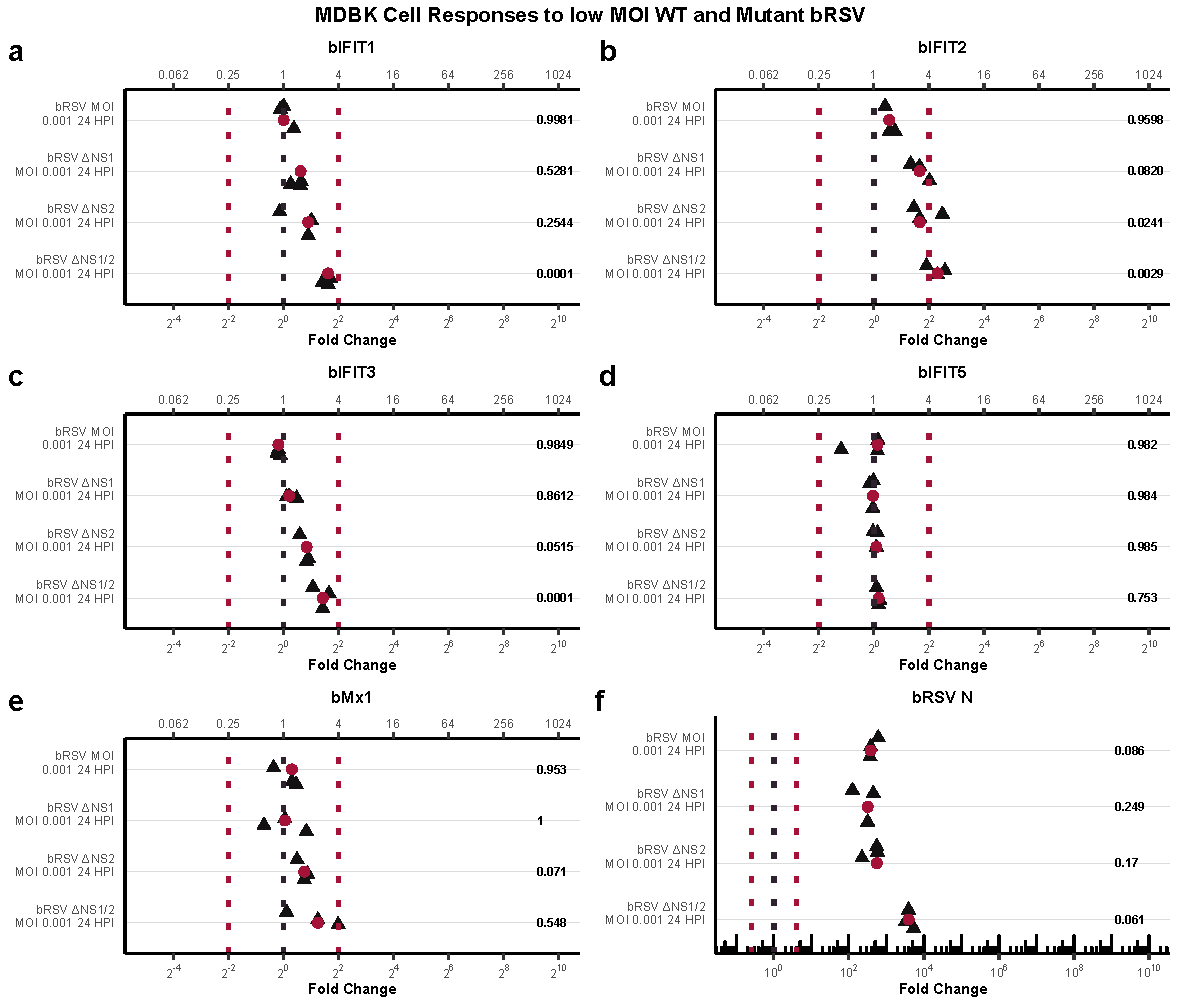
\includegraphics[width=1\linewidth]{07. Chapter 2/Figs/02. Induction/06. mdbk_brsv_low_moi.pdf}
    \caption[MDBK \textit{bIFIT} Response to Low MOI bRSV Infections.]{\textbf{MDBK \textit{bIFIT} Response to Low MOI bRSV Infections.} (a) \textit{bIFIT1}, (b) \textit{bIFIT2}, (c) \textit{bIFIT3}, (d) \textit{bIFIT5}, (e) \textit{bMx1}, and (f) \textit{bRSV N} gene expression levels were assessed using quantitative real-time PCR (qPCR) in MDBK cell line following infection with WT or \(\Delta\)NS1, \(\Delta\)NS2, and \(\Delta\)NS1/2 bRSV at MOIs of 0.001 for 24 hours post-infection. Relative expression values are normalized to standardized mock-treated samples. Median values are represented by red circles. The black dotted line represents mock expression levels, while the red dotted lines indicate biologically significant induction thresholds. Numeric values indicate the p-values compared to mock-treated samples.}
    \label{fig:MDBK responses to low MOI mutant bRSV}
\end{figure}

Continuing the investigation, we utilized 0.001 MOI \(\Delta\)NS1, \(\Delta\)NS2, and \(\Delta\)NS1/2 bRSV along with 0.001 MOI WT bRSV as a control to assess their potential involvement in the suppression of \textit{bIFIT} induction. As illustrated in Figure \ref{fig:MDBK responses to low MOI mutant bRSV}, none of the genes of interest were influenced by WT infection, in line with our previous observations. Concerning the mutant viruses, \textit{bIFIT5} was unresponsive to any of them, while the other genes exhibited marginal induction in at least one condition. Notably, \(\Delta\)NS1 infection influenced only \textit{bIFIT2}, inducing it nearly to biologically significant levels at around 3.8-fold. The absence of NS2 protein caused minor induction in all tested genes, except for \textit{bIFIT5}, approximately a 2-fold increase for \textit{bIFIT1}, \textit{bIFIT3}, and \textit{bMx1}, and a 3.8-fold induction for \textit{bIFIT2}. The infection with the double deletion mutant \(\Delta\)NS1/2 bRSV resulted in the most robust response, inducing \textit{bIFIT1} and \textit{bIFIT3} at 3.8-fold, \textit{bMx1} at 3-fold, and notably, a biologically significant induction of \textit{bIFIT2} at 5-fold. Regarding data distribution, the \textit{bIFIT5}, \textit{bRSV N}, and \textit{bMx1} datasets exhibited a normal distribution of data with unequal variances, while the \textit{bIFIT1}, \textit{bIFIT2}, and \textit{bIFIT3} datasets exhibited normal distributions with equal variances. This data suggests that, except for \textit{bIFIT5}, bRSV NS proteins negatively influence the induction of \textit{bIFITs} and \textit{bMx1}, with NS2 seemingly a more potent inhibitor.

\begin{figure}
    \centering
    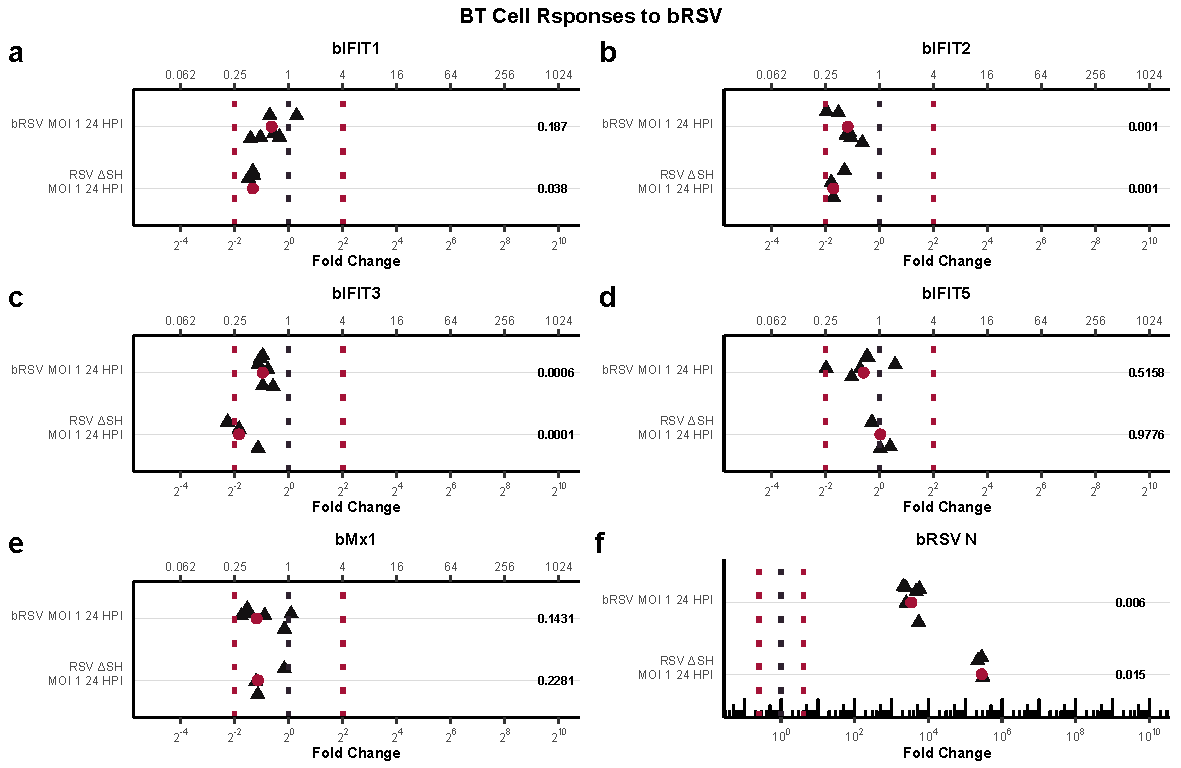
\includegraphics[width=1\linewidth]{07. Chapter 2/Figs/02. Induction/09. bt_brsv.pdf}
    \caption[BT \textit{bIFIT} Response to WT and \(\Delta\)SH bRSV Infection.]{\textbf{BT \textit{bIFIT} Response to WT and \(\Delta\)SH bRSV Infection.} (a) \textit{bIFIT1}, (b) \textit{bIFIT2}, (c) \textit{bIFIT3}, (d) \textit{bIFIT5}, (e) \textit{bMx1}, and (f) \textit{bRSV N} gene expression levels were assessed using quantitative real-time PCR (qPCR) in BT cell line following infection with WT or \(\Delta\)SH bRSV at MOI 1 for 24 hours post-infection. Relative expression values are normalized to standardized mock-treated samples. Median values are represented by red circles. The black dotted line represents mock expression levels, while the red dotted lines indicate biologically significant induction thresholds. Numeric values indicate the p-values compared to mock-treated samples.}
    \label{fig:BT responses to bRSV}
\end{figure}

Finally, we aimed to partially validate the bRSV infection data using the BT cell line. The cells were infected with crudely extracted WT and \(\Delta\)SH bRSV at an MOI of 1 for 24 hours. The relevant data is depicted in Figure \ref{fig:BT responses to bRSV}. It's noteworthy that all datasets exhibited normal distribution and equal variance except for \textit{bIFIT1} and \textit{bRSV N}. In general, a reduction in mRNA levels was observed as a consequence of infection, regardless of the virus used. Specifically, WT bRSV infection led to a \(2^{-0.5}\)-fold decrease for \textit{bIFIT1} and \textit{bIFIT5}, a \(2^{-1}\)-fold decrease for \textit{bIFIT2} and \textit{bIFIT3}, and a \(2^{-1.5}\)-fold decrease for \textit{bMx1}. Infection with \(\Delta\)SH bRSV resulted in approximately a \(2^{-1.5}\)-fold decrease in the levels of \textit{bIFIT1} and \textit{bMx1}, a biologically significant decrease of \(2^{-2}\)-fold for \textit{bIFIT2} and \textit{bIFIT3}, and no alteration in \textit{bIFIT5} mRNA levels. Overall, the presence of the SH protein appears to stimulate the induction of \textit{bIFIT} and \textit{bMx1}. This contrasts with observations in the MDBK cell line, where no differences were observed in the induction potential of WT and \(\Delta\)SH bRSV, except for \textit{bIFIT2}, which was significantly upregulated in the absence of the SH protein (Figure \ref{fig:MDBK responses to dSH}).

\subsection{Bovine \textit{IFITs} Responses to hRSV Infection} \label{subsec:Bovine IFITs Responses to hRSV Infection}
We sought to investigate potential cross-species protection between hRSV and bRSV. As detailed in Section \ref{subsec:Human IFITs Responses to bRSV}, bRSV induces \textit{hIFITs} to a level surpassing that of equivalent hRSV infection in the A549 cell line, suggesting cross-protection of human cells to both viruses. While minimal \textit{bIFIT} or \textit{bMx1} responses were observed to WT or mutant bRSV infections in the MDBK and BT cell lines, we aimed to assess the potential response to hRSV. Furthermore, as noted in Section \ref{subsec:Human IFITs Responses to Human RSV}, the purification methodology for isolating hRSV influenced \textit{hIFIT} induction, with ultrapurified preparations causing higher levels of induction. Considering these factors, MDBK and BT cells were infected with crude extracted and ultracentrifugation-purified hRSV at an MOI of 1 for 24 hours. Subsequently, cells were lysed, mRNA was extracted and converted into cDNA, and transcripts were quantified using RT-qPCR.

\begin{figure}
    \centering
    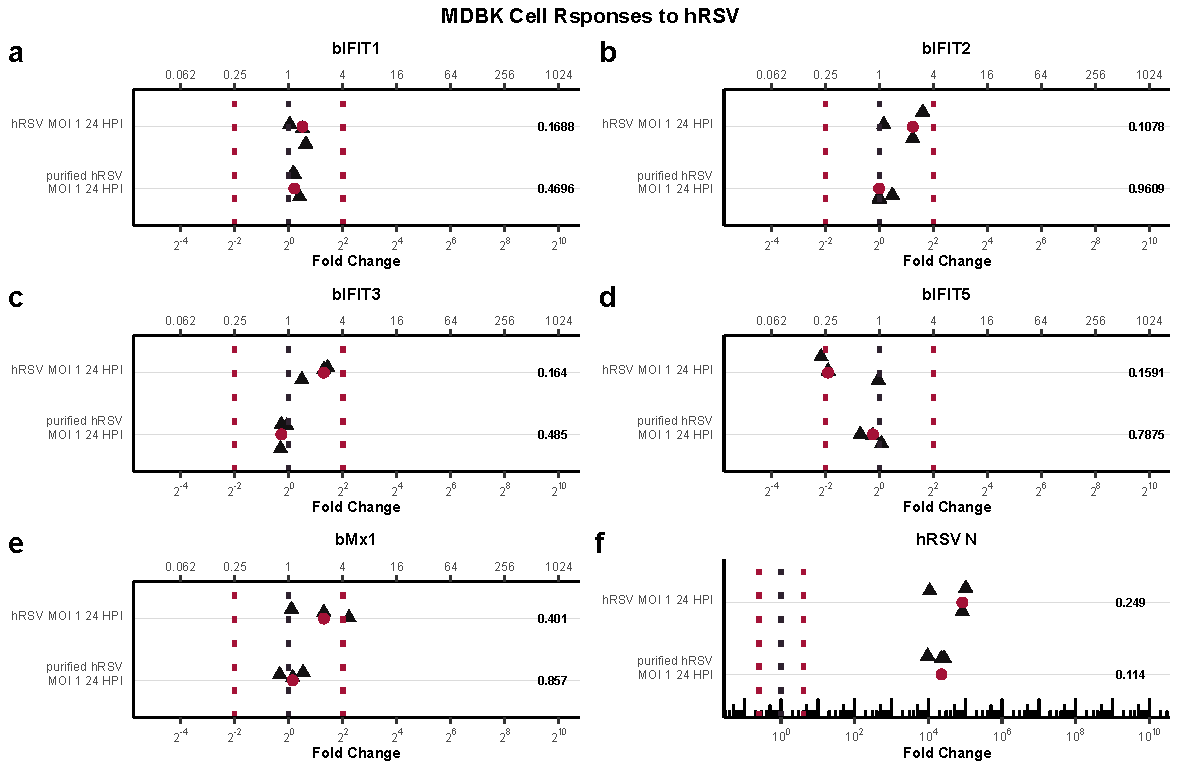
\includegraphics[width=1\linewidth]{07. Chapter 2/Figs/02. Induction/07. mdbk_hrsv.pdf}
    \caption[MDBK \textit{bIFIT} Response to Crude-Extracted and Ultra-Purified hRSV Infection.]{\textbf{MDBK \textit{bIFIT} Response to Crude-Extracted and Ultra-Purified hRSV Infection.} (a) \textit{bIFIT1}, (b) \textit{bIFIT2}, (c) \textit{bIFIT3}, (d) \textit{bIFIT5}, (e) \textit{bMx1}, and (f) \textit{hRSV N} gene expression levels were assessed using quantitative real-time PCR (qPCR) in MDBK cell line following infection with crude-extraccted and ultra-purified hRSV at MOI 1 for 24 hours post-infection. Relative expression values are normalized to standardized mock-treated samples. Median values are represented by red circles. The black dotted line represents mock expression levels, while the red dotted lines indicate biologically significant induction thresholds. Numeric values indicate the p-values compared to mock-treated samples.}
    \label{fig:bIFIT responses to hRSV infection in MDBK}
\end{figure}

Figure \ref{fig:bIFIT responses to hRSV infection in MDBK} illustrates the responses of \textit{bIFITs} and \textit{bMx1} to hRSV in MDBK cells. Both viral preparations successfully replicated, as evidenced by the quantification of \textit{hRSV N} (Panel f; \(2^{5}\)-fold and \(2^{4.2}\)-fold increases, respectively), albeit unexpectedly exhibiting an order of magnitude difference in the final fold changes. Notably, ultrapurified hRSV infection did not influence the relative levels of any tested genes. In contrast, crude extracted hRSV infection induced a variety of effects: a modest induction of \textit{bIFIT1} by 1.5-fold, and \textit{bIFIT2}, \textit{bIFIT3}, and \textit{bMx1} by 3-fold, alongside a significant downregulation of \textit{bIFIT5} by \(2^{-2}\)-fold. The datasets for \textit{bIFIT1}, \textit{bIFIT2}, and \textit{bIFIT3} exhibited normal distribution with equal variances, while the rest displayed normal distributions with unequal variances.

\begin{figure}
    \centering
    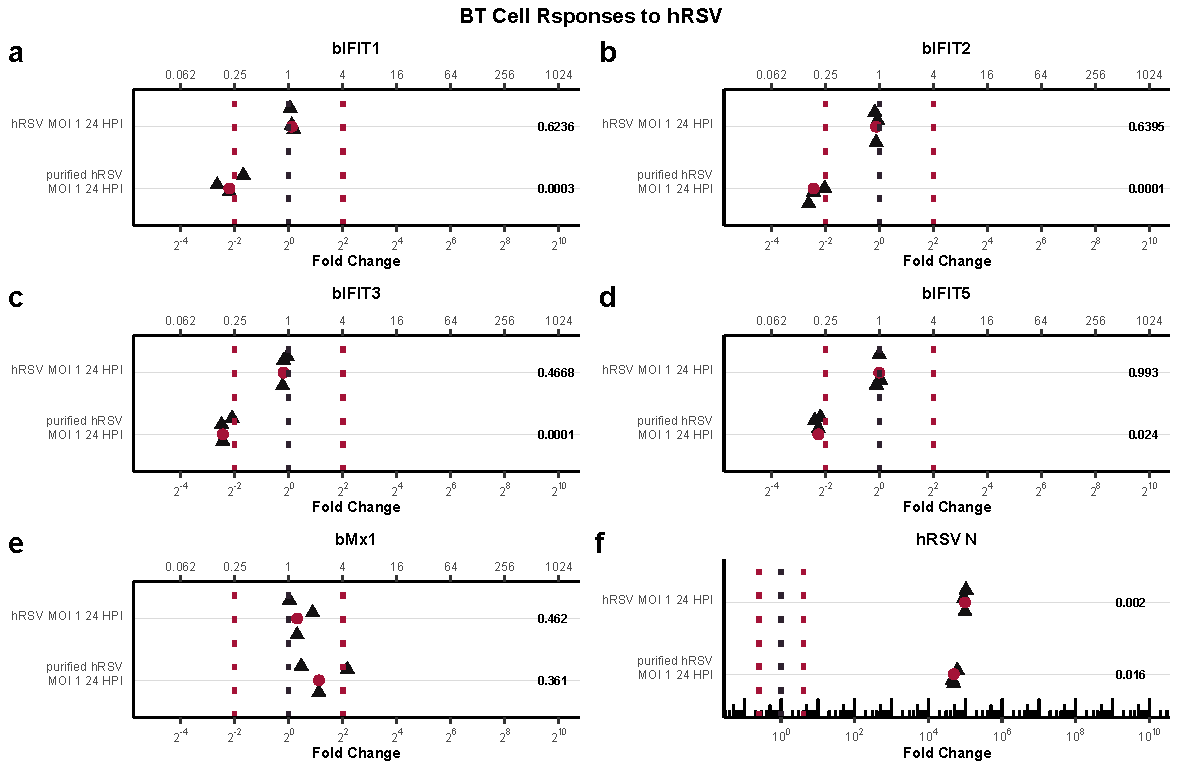
\includegraphics[width=1\linewidth]{07. Chapter 2/Figs/02. Induction/10. bt_hrsv.pdf}
    \caption[BT \textit{bIFIT} Response to Crude-Extracted and Ultra-Purified hRSV Infection.]{\textbf{BT \textit{bIFIT} Response to Crude-Extracted and Ultra-Purified hRSV Infection.} (a) \textit{bIFIT1}, (b) \textit{bIFIT2}, (c) \textit{bIFIT3}, (d) \textit{bIFIT5}, (e) \textit{bMx1}, and (f) \textit{hRSV N} gene expression levels were assessed using quantitative real-time PCR (qPCR) in BT cell line following infection with crude-extraccted and ultra-purified hRSV at MOI 1 for 24 hours post-infection. Relative expression values are normalized to standardized mock-treated samples. Median values are represented by red circles. The black dotted line represents mock expression levels, while the red dotted lines indicate biologically significant induction thresholds. Numeric values indicate the p-values compared to mock-treated samples.}
    \label{fig:Bt responses to hRSV}
\end{figure}

Results from BT cells infected with hRSV are depicted in Figure \ref{fig:Bt responses to hRSV}. Similar to MDBK cells, hRSV successfully infected and replicated in BT cells. Interestingly, the effect observed in MDBK cells (Figure \ref{fig:bIFIT responses to hRSV infection in MDBK}) was reversed: the crude extracted viral preparation did not influence the expression of the genes of interest, while ultra-purified hRSV caused significant effects. It led to a biologically substantial downregulation of \textit{bIFIT1}, \textit{bIFIT2}, \textit{bIFIT3}, and \textit{bIFIT5} by \(2^{-2.5}\)-fold, and induced \textit{bMx1} by 2-fold. Normal distribution with equal variances was observed for \textit{bIFIT1} and \textit{bIFIT2} datasets, while the others exhibited normal distributions with unequal variances.

\section{Conclusions} \label{sec:Conclusions Chapter2}
A summary of \textit{bIFIT} induction trends following the treatment with bIFN$\upalpha$ and LPS can be seen in Table \ref{tab:Summary of Bovine IFIT Responses to Activators of Innate Immune Response.}. We verified the responsiveness of both MDBK and BT cell lines to bovine IFN$\upalpha$, demonstrating competence in inducing \textit{bIFIT} and \textit{bMx1}. Similar to the observations with \textit{hIFITs}, where LPS barely induced \textit{hIFITs} to biologically significant levels, LPS failed to induce \textit{bIFITs} in the MDBK cell line. However, the literature confirms that MDBK can sense and respond to LPS \cite{Cui2022ThePathway}, suggesting either LPS not being physiologically involved with \textit{bIFIT} induction, or the use of insufficient concentration and the improper time of treatment to observe an effect. Extensive experimentation revealed either no or only minimal induction of bovine \textit{IFITs} by bRSV infection. The summary tables of bovine \textit{IFIT} induction trends by wild type and mutant bRSV infection can be seen in Table \ref{tab:Summary of Bovine IFIT Responses to Wild Type bRSV Infection.} and Table \ref{tab:Summary of Bovine IFIT Responses to Mutant bRSV Infection.} respectively. Our data suggests that WT bRSV does not influence \textit{bIFIT} induction, whereas ultrapurified WT bRSV induces \textit{bMx1} expression. This discrepancy might be attributed to cellular contaminants present in crudely extracted WT bRSV, hindering the induction of this gene. Another explanation could be that during the ultrapurification process, a specific RSV population with distinct virion morphology was selected, meaning the final viral prep was composed of either only spherical or only filamentous virions, causing the observed outcomes. In the MDBK cell line, we observed specific inhibition of \textit{bIFIT2} induction by SH and NS1 bRSV proteins. Infection with mutant bRSV lacking these proteins resulted in a mild but biologically significant induction. Conversely, the NS2 protein appears to inhibit the induction of \textit{bIFIT1}, \textit{bIFIT2}, and \textit{bIFIT3}, with both NS1 and NS2 potentially acting synergistically. In the BT cell line, while WT bRSV failed to induce \textit{bIFITs}, $\Updelta$SH bRSV caused a biologically significant downregulation of \textit{bIFIT} mRNA levels, presenting a puzzling phenotype. Collectively, it appears that there are elements within bRSV inhibiting the induction of \textit{bIFITs} and \textit{bMx1}. However, these inhibitory effects were not observed in human cell lines, suggesting differential human and bovine \textit{IFIT} induction pathways, which bRSV inhibits in the bovine cell lines.

\begin{table}
    \centering
    \begin{tabular}{lllll}
    \hline
        \textbf{Cell Line} & \textbf{IFIT} & \textbf{Treatment} & \textbf{Figure} & \textbf{Trend} \\ \hline
        MDBK & IFIT1 & bIFN$\upalpha$ 5 ng/mL 3h & Figure 4.4 & \(\uparrow\) \\ 
        MDBK & IFIT1 & bIFN$\upalpha$ 5 ng/mL 6h & Figure 4.4 & \(\uparrow\) \\ 
        MDBK & IFIT1 & LPS 0.5 ng/mL 6h & Figure 4.5 & \(\rightarrow\) \\ 
        MDBK & IFIT1 & LPS 1 ng/mL 6h & Figure 4.5 & \(\rightarrow\) \\ 
        MDBK & IFIT1 & LPS 2.5 ng/mL 6h & Figure 4.5 & \(\searrow\) \\ 
        MDBK & IFIT1 & LPS 5 ng/mL 6h & Figure 4.5 & \(\rightarrow\) \\ 
        MDBK & IFIT1 & LPS 10 ng/mL 6h & Figure 4.5 & \(\rightarrow\) \\ 
        BT & IFIT1 & bIFN$\upalpha$ 5 ng/mL 3h & Figure 4.6 & \(\uparrow\) \\ 
        BT & IFIT1 & bIFN$\upalpha$ 5 ng/mL 24h & Figure 4.6 & \(\rightarrow\) \\ 
        MDBK & IFIT2 & bIFN$\upalpha$ 5 ng/mL 3h & Figure 4.4 & \(\uparrow\) \\ 
        MDBK & IFIT2 & bIFN$\upalpha$ 5 ng/mL 6h & Figure 4.4 & \(\nearrow\) \\ 
        MDBK & IFIT2 & LPS 0.5 ng/mL 6h & Figure 4.5 & \(\rightarrow\) \\ 
        MDBK & IFIT2 & LPS 1 ng/mL 6h & Figure 4.5 & \(\rightarrow\) \\ 
        MDBK & IFIT2 & LPS 2.5 ng/mL 6h & Figure 4.5 & \(\rightarrow\) \\ 
        MDBK & IFIT2 & LPS 5 ng/mL 6h & Figure 4.5 & \(\rightarrow\) \\ 
        MDBK & IFIT2 & LPS 10 ng/mL 6h & Figure 4.5 & \(\rightarrow\) \\ 
        BT & IFIT2 & bIFN$\upalpha$ 5 ng/mL 3h & Figure 4.6 & \(\rightarrow\) \\ 
        BT & IFIT2 & bIFN$\upalpha$ 5 ng/mL 24h & Figure 4.6 & \(\rightarrow\) \\ 
        MDBK & IFIT3 & bIFN$\upalpha$ 5 ng/mL 3h & Figure 4.4 & \(\uparrow\) \\ 
        MDBK & IFIT3 & bIFN$\upalpha$ 5 ng/mL 6h & Figure 4.4 & \(\nearrow\) \\ 
        MDBK & IFIT3 & LPS 0.5 ng/mL 6h & Figure 4.5 & \(\rightarrow\) \\ 
        MDBK & IFIT3 & LPS 1 ng/mL 6h & Figure 4.5 & \(\rightarrow\) \\ 
        MDBK & IFIT3 & LPS 2.5 ng/mL 6h & Figure 4.5 & \(\searrow\) \\ 
        MDBK & IFIT3 & LPS 5 ng/mL 6h & Figure 4.5 & \(\rightarrow\) \\ 
        MDBK & IFIT3 & LPS 10 ng/mL 6h & Figure 4.5 & \(\rightarrow\) \\ 
        BT & IFIT3 & bIFN$\upalpha$ 5 ng/mL 3h & Figure 4.6 & \(\uparrow\) \\ 
        BT & IFIT3 & bIFN$\upalpha$ 5 ng/mL 24h & Figure 4.6 & \(\rightarrow\) \\ 
        MDBK & IFIT5 & bIFN$\upalpha$ 5 ng/mL 3h & Figure 4.4 & \(\nearrow\) \\ 
        MDBK & IFIT5 & bIFN$\upalpha$ 5 ng/mL 6h & Figure 4.4 & \(\nearrow\) \\ 
        MDBK & IFIT5 & LPS 0.5 ng/mL 6h & Figure 4.5 & \(\rightarrow\) \\ 
        MDBK & IFIT5 & LPS 1 ng/mL 6h & Figure 4.5 & \(\rightarrow\) \\ 
        MDBK & IFIT5 & LPS 2.5 ng/mL 6h & Figure 4.5 & \(\rightarrow\) \\ 
        MDBK & IFIT5 & LPS 5 ng/mL 6h & Figure 4.5 & \(\rightarrow\) \\ 
        MDBK & IFIT5 & LPS 10 ng/mL 6h & Figure 4.5 & \(\rightarrow\) \\ 
        BT & IFIT5 & bIFN$\upalpha$ 5 ng/mL 3h & Figure 4.6 & \(\nearrow\) \\ 
        BT & IFIT5 & bIFN$\upalpha$ 5 ng/mL 24h & Figure 4.6 & \(\rightarrow\) \\ \hline
    \end{tabular}
	\caption[Summary of Bovine \textit{IFIT} Responses to Activators of Innate Immune Response.]{\textbf{Summary of Bovine \textit{IFIT} Responses to Activators of Innate Immune Response.} Trend arrows indicate abundance relative to mock-treated values: strong downregulation ($\downarrow$, 0.062-0.25); mild downregulation ($\searrow$, 0.25-0.5); no difference ($\rightarrow$, 0.5-1.5); mild upregulation ($\nearrow$, 1.5-4); moderate upregulation ($\uparrow$, 4-64); strong upregulation ($\uparrow\uparrow$, 64-258); very strong upregulation ($\uparrow\uparrow\uparrow$, 258-1024).}
    \label{tab:Summary of Bovine IFIT Responses to Activators of Innate Immune Response.}
\end{table}

\begin{table}
    \centering
    \begin{tabular}{lllll}
    \hline
	\textbf{IFIT} & \textbf{Treatment} & \textbf{Figure} & \textbf{Trend} \\ \hline
        IFIT1 & bRSV MOI 0.1 24 HPI & Figure 4.7 & \(\rightarrow\) \\ \hline
        IFIT1 & bRSV MOI 0.1 48 HPI & Figure 4.7 & \(\nearrow\) \\ 
        IFIT1 & bRSV MOI 1 24 HPI & Figure 4.7 & \(\rightarrow\) \\ 
        IFIT1 & bRSV MOI 1 48 HPI & Figure 4.7 & \(\nearrow\) \\ 
        IFIT1 & bRSV MOI 2 24 HPI & Figure 4.7 & \(\rightarrow\) \\ 
        IFIT1 & bRSV MOI 2 48 HPI & Figure 4.7 & \(\searrow\) \\ 
        IFIT1 & purified bRSV MOI 1 24 HPI & Figure 4.8 & \(\rightarrow\) \\ 
        IFIT1 & purified bRSV MOI 1 24 HPI with ruxolitinib & Figure 4.8 & \(\rightarrow\) \\ 
        IFIT1 & purified UV inactivated bRSV MOI 1 24 HPI & Figure 4.8 & \(\searrow\) \\ 
        IFIT2 & bRSV MOI 0.1 24 HPI & Figure 4.7 & \(\rightarrow\) \\ 
        IFIT2 & bRSV MOI 0.1 48 HPI & Figure 4.7 & \(\rightarrow\) \\ 
        IFIT2 & bRSV MOI 1 24 HPI & Figure 4.7 & \(\rightarrow\) \\ 
        IFIT2 & bRSV MOI 1 48 HPI & Figure 4.7 & \(\rightarrow\) \\ 
        IFIT2 & bRSV MOI 2 24 HPI & Figure 4.7 & \(\rightarrow\) \\ 
        IFIT2 & bRSV MOI 2 48 HPI & Figure 4.7 & \(\searrow\) \\ 
        IFIT2 & purified bRSV MOI 1 24 HPI & Figure 4.8 & \(\rightarrow\) \\ 
        IFIT2 & purified bRSV MOI 1 24 HPI with ruxolitinib & Figure 4.8 & \(\rightarrow\) \\ 
        IFIT2 & purified UV inactivated bRSV MOI 1 24 HPI & Figure 4.8 & \(\rightarrow\) \\ 
        IFIT3 & bRSV MOI 0.1 24 HPI & Figure 4.7 & \(\rightarrow\) \\ 
        IFIT3 & bRSV MOI 0.1 48 HPI & Figure 4.7 & \(\rightarrow\) \\ 
        IFIT3 & bRSV MOI 1 24 HPI & Figure 4.7 & \(\rightarrow\) \\ 
        IFIT3 & bRSV MOI 1 48 HPI & Figure 4.7 & \(\rightarrow\) \\ 
        IFIT3 & bRSV MOI 2 24 HPI & Figure 4.7 & \(\rightarrow\) \\ 
        IFIT3 & bRSV MOI 2 48 HPI & Figure 4.7 & \(\rightarrow\) \\ 
        IFIT3 & purified bRSV MOI 1 24 HPI & Figure 4.8 & \(\rightarrow\) \\ 
        IFIT3 & purified bRSV MOI 1 24 HPI with ruxolitinib & Figure 4.8 & \(\rightarrow\) \\ 
        IFIT3 & purified UV inactivated bRSV MOI 1 24 HPI & Figure 4.8 & \(\rightarrow\) \\ 
        IFIT5 & bRSV MOI 0.1 24 HPI & Figure 4.7 & \(\rightarrow\) \\ 
        IFIT5 & bRSV MOI 0.1 48 HPI & Figure 4.7 & \(\rightarrow\) \\ 
        IFIT5 & bRSV MOI 1 24 HPI & Figure 4.7 & \(\rightarrow\) \\ 
        IFIT5 & bRSV MOI 1 48 HPI & Figure 4.7 & \(\rightarrow\) \\ 
        IFIT5 & bRSV MOI 2 24 HPI & Figure 4.7 & \(\rightarrow\) \\ 
        IFIT5 & bRSV MOI 2 48 HPI & Figure 4.7 & \(\rightarrow\) \\ 
        IFIT5 & purified bRSV MOI 1 24 HPI & Figure 4.8 & \(\rightarrow\) \\ 
        IFIT5 & purified bRSV MOI 1 24 HPI with ruxolitinib & Figure 4.8 & \(\rightarrow\) \\ 
        IFIT5 & purified UV inactivated bRSV MOI 1 24 HPI & Figure 4.8 & \(\rightarrow\) \\ \hline
    \end{tabular}
	\caption[Summary of Bovine \textit{IFIT} Responses to Wild Type bRSV Infection.]{\textbf{Summary of Bovine \textit{IFIT} Responses to Wild Type bRSV Infection.} Trend arrows indicate abundance relative to mock-treated values: strong downregulation ($\downarrow$, 0.062-0.25); mild downregulation ($\searrow$, 0.25-0.5); no difference ($\rightarrow$, 0.5-1.5); mild upregulation ($\nearrow$, 1.5-4); moderate upregulation ($\uparrow$, 4-64); strong upregulation ($\uparrow\uparrow$, 64-258); very strong upregulation ($\uparrow\uparrow\uparrow$, 258-1024).}
    \label{tab:Summary of Bovine IFIT Responses to Wild Type bRSV Infection.}
\end{table}

\begin{table}
    \centering
    \begin{tabular}{lllll}
    \hline
	\textbf{Cell Line} & \textbf{IFIT} & \textbf{Treatment} & \textbf{Figure} & \textbf{Trend} \\ \hline
        MDBK & IFIT1 & bRSV MOI 1 24 HPI & Figure 4.9 & \(\rightarrow\) \\ 
        MDBK & IFIT1 & bRSV $\Updelta$SH MOI 1 24 HPI & Figure 4.9 & \(\rightarrow\) \\ 
        MDBK & IFIT1 & bRSV MOI 0.001 24 HPI & Figure 4.10 & \(\rightarrow\) \\ 
        MDBK & IFIT1 & bRSV $\Updelta$NS1 MOI 0.001 24 HPI & Figure 4.10 & \(\rightarrow\) \\ 
        MDBK & IFIT1 & bRSV $\Updelta$NS2 MOI 0.001 24 HPI & Figure 4.10 & \(\nearrow\) \\ 
        MDBK & IFIT1 & bRSV $\Updelta$NS1/2 MOI 0.001 24 HPI & Figure 4.10 & \(\nearrow\) \\ 
        BT & IFIT1 & bRSV MOI 1 24 HPI & Figure 4.11 & \(\rightarrow\) \\ 
        BT & IFIT1 & bRSV $\Updelta$SH MOI 1 24 HPI & Figure 4.11 & \(\searrow\) \\ 
        MDBK & IFIT2 & bRSV MOI 1 24 HPI & Figure 4.9 & \(\rightarrow\) \\ 
        MDBK & IFIT2 & bRSV $\Updelta$SH MOI 1 24 HPI & Figure 4.9 & \(\nearrow\) \\ 
        MDBK & IFIT2 & bRSV MOI 0.001 24 HPI & Figure 4.10 & \(\rightarrow\) \\ 
        MDBK & IFIT2 & bRSV $\Updelta$NS1 MOI 0.001 24 HPI & Figure 4.10 & \(\nearrow\) \\ 
        MDBK & IFIT2 & bRSV $\Updelta$NS2 MOI 0.001 24 HPI & Figure 4.10 & \(\nearrow\) \\ 
        MDBK & IFIT2 & bRSV $\Updelta$NS1/2 MOI 0.001 24 HPI & Figure 4.10 & \(\uparrow\) \\ 
        BT & IFIT2 & bRSV MOI 1 24 HPI & Figure 4.11 & \(\searrow\) \\ 
        BT & IFIT2 & bRSV $\Updelta$SH MOI 1 24 HPI & Figure 4.11 & \(\searrow\) \\ 
        MDBK & IFIT3 & bRSV MOI 1 24 HPI & Figure 4.9 & \(\rightarrow\) \\ 
        MDBK & IFIT3 & bRSV $\Updelta$SH MOI 1 24 HPI & Figure 4.9 & \(\nearrow\) \\ 
        MDBK & IFIT3 & bRSV MOI 0.001 24 HPI & Figure 4.10 & \(\rightarrow\) \\ 
        MDBK & IFIT3 & bRSV $\Updelta$NS1 MOI 0.001 24 HPI & Figure 4.10 & \(\rightarrow\) \\ 
        MDBK & IFIT3 & bRSV $\Updelta$NS2 MOI 0.001 24 HPI & Figure 4.10 & \(\nearrow\) \\ 
        MDBK & IFIT3 & bRSV $\Updelta$NS1/2 MOI 0.001 24 HPI & Figure 4.10 & \(\nearrow\) \\ 
        BT & IFIT3 & bRSV MOI 1 24 HPI & Figure 4.11 & \(\searrow\) \\ 
        BT & IFIT3 & bRSV $\Updelta$SH MOI 1 24 HPI & Figure 4.11 & \(\downarrow\) \\ 
        MDBK & IFIT5 & bRSV MOI 1 24 HPI & Figure 4.9 & \(\rightarrow\) \\ 
        MDBK & IFIT5 & bRSV $\Updelta$SH MOI 1 24 HPI & Figure 4.9 & \(\rightarrow\) \\ 
        MDBK & IFIT5 & bRSV MOI 0.001 24 HPI & Figure 4.10 & \(\rightarrow\) \\ 
        MDBK & IFIT5 & bRSV $\Updelta$NS1 MOI 0.001 24 HPI & Figure 4.10 & \(\rightarrow\) \\ 
        MDBK & IFIT5 & bRSV $\Updelta$NS2 MOI 0.001 24 HPI & Figure 4.10 & \(\rightarrow\) \\ 
        MDBK & IFIT5 & bRSV $\Updelta$NS1/2 MOI 0.001 24 HPI & Figure 4.10 & \(\rightarrow\) \\ 
        BT & IFIT5 & bRSV MOI 1 24 HPI & Figure 4.11 & \(\rightarrow\) \\ 
        BT & IFIT5 & bRSV $\Updelta$SH MOI 1 24 HPI & Figure 4.11 & \(\rightarrow\) \\ \hline
    \end{tabular}
	\caption[Summary of Bovine \textit{IFIT} Responses to Mutant bRSV Infection.]{\textbf{Summary of Bovine \textit{IFIT} Responses to Mutant bRSV Infection.} Trend arrows indicate abundance relative to mock-treated values: strong downregulation ($\downarrow$, 0.062-0.25); mild downregulation ($\searrow$, 0.25-0.5); no difference ($\rightarrow$, 0.5-1.5); mild upregulation ($\nearrow$, 1.5-4); moderate upregulation ($\uparrow$, 4-64); strong upregulation ($\uparrow\uparrow$, 64-258); very strong upregulation ($\uparrow\uparrow\uparrow$, 258-1024).}
    \label{tab:Summary of Bovine IFIT Responses to Mutant bRSV Infection.}
\end{table}

Furthermore, we aimed to explore if the observed host restriction of RSV \textit{in vivo} could be attributed to induced \textit{bIFIT} expression, akin to what was observed with \textit{hIFITs} (Section \ref{subsec:Human IFITs Responses to bRSV}). The summary of bovine \textit{IFIT} induction trends by hRSV infection can be seen in Table \ref{tab:Summary of Bovine IFIT Responses to hRSV Infection.} The investigation also aimed to determine whether the inability to induce \textit{bIFITs} by bRSV is specific to that virus. Notably, we observed no biologically significant induction of \textit{bIFITs} in either the MDBK or BT cell lines. Additionally, we noted that the purification procedure substantially influenced the differential expression of \textit{bIFITs} and exhibited notable differences between the two cell lines. For instance, although ultrapurified hRSV did not affect \textit{bIFIT} levels in the MDBK cell line, crude extracted hRSV marginally induced \textit{bIFIT1}, \textit{bIFIT2}, and \textit{bIFIT3}, while significantly inhibiting \textit{bIFIT5} induction. Conversely, crudely extracted hRSV did not influence \textit{bIFIT} expression in the BT cell line, whereas infection with ultrapurified hRSV biologically significantly downregulated all \textit{bIFITs}. Intriguingly, taking into account also data from Chapter \ref{ch:Assessment of Transcriptional Induction of Human IFITs in the Context of RSV}, both hRSV and bRSV efficiently replicated in cells of the other species, as confirmed by RSV \textit{N} gene quantification. This suggests that the reported species restriction of RSV \textit{in vivo} is not recapitulated in our \textit{in vitro} experiments. Consequently, this implies that species restriction arises from humoral and cell-mediated immune responses rather than differences in intracellular antiviral proteins between species.

\begin{table}
    \centering
    \begin{tabular}{lllll}
    \hline
		\textbf{Cell Line} & \textbf{IFIT} & \textbf{Treatment} & \textbf{Figure} & \textbf{Trend} \\ \hline
        MDBK & IFIT1 & hRSV MOI 1 24 HPI & Figure 4.12 & \(\rightarrow\) \\ 
        MDBK & IFIT1 & purified hRSV MOI 1 24 HPI & Figure 4.12 & \(\rightarrow\) \\ 
        BT & IFIT1 & hRSV MOI 1 24 HPI & Figure 4.13 & \(\rightarrow\) \\ 
        BT & IFIT1 & purified hRSV MOI 1 24 HPI & Figure 4.13 & \(\downarrow\) \\ 
        MDBK & IFIT2 & hRSV MOI 1 24 HPI & Figure 4.12 & \(\nearrow\) \\ 
        MDBK & IFIT2 & purified hRSV MOI 1 24 HPI & Figure 4.12 & \(\rightarrow\) \\ 
        BT & IFIT2 & hRSV MOI 1 24 HPI & Figure 4.13 & \(\rightarrow\) \\ 
        BT & IFIT2 & purified hRSV MOI 1 24 HPI & Figure 4.13 & \(\downarrow\) \\ 
        MDBK & IFIT3 & hRSV MOI 1 24 HPI & Figure 4.12 & \(\nearrow\) \\ 
        MDBK & IFIT3 & purified hRSV MOI 1 24 HPI & Figure 4.12 & \(\rightarrow\) \\ 
        BT & IFIT3 & hRSV MOI 1 24 HPI & Figure 4.13 & \(\rightarrow\) \\ 
        BT & IFIT3 & purified hRSV MOI 1 24 HPI & Figure 4.13 & \(\downarrow\) \\ 
        MDBK & IFIT5 & hRSV MOI 1 24 HPI & Figure 4.12 & \(\downarrow\) \\ 
        MDBK & IFIT5 & purified hRSV MOI 1 24 HPI & Figure 4.12 & \(\rightarrow\) \\ 
        BT & IFIT5 & hRSV MOI 1 24 HPI & Figure 4.13 & \(\rightarrow\) \\ 
        BT & IFIT5 & purified hRSV MOI 1 24 HPI & Figure 4.13 & \(\downarrow\) \\ \hline
    \end{tabular}
	\caption[Summary of Bovine \textit{IFIT} Responses to hRSV Infection.]{\textbf{Summary of Bovine \textit{IFIT} Responses to hRSV Infection.} Trend arrows indicate abundance relative to mock-treated values: strong downregulation ($\downarrow$, 0.062-0.25); mild downregulation ($\searrow$, 0.25-0.5); no difference ($\rightarrow$, 0.5-1.5); mild upregulation ($\nearrow$, 1.5-4); moderate upregulation ($\uparrow$, 4-64); strong upregulation ($\uparrow\uparrow$, 64-258); very strong upregulation ($\uparrow\uparrow\uparrow$, 258-1024).}
    \label{tab:Summary of Bovine IFIT Responses to hRSV Infection.}
\end{table}

Taken together, these findings suggest that either \textit{bIFITs} might not be involved in human and bovine RSV infection, or the chosen cell lines for the experiments might not accurately represent the \textit{in vivo} scenario. In addressing these queries, we referred to the literature and found two related RNAseq experiments exploring the differentially expressed genes from bronchial lymph nodes or whole blood of dairy calves. These studies identified all bovine \textit{IFITs} as differentially expressed in the former, while \textit{bIFIT2} and \textit{bIFIT5} transcripts were detected as differentially expressed in whole blood \cite{Johnston2019ExperimentalResponse., Johnston2021MessengerCalves}. Collectively, it appears that all bovine \textit{IFITs} are induced \textit{in vivo}, indicating their potential involvement in bRSV replication restriction, similar to what is observed with human \textit{IFITs}.

The outstanding question that remains to be answered is why we failed to detect \textit{bIFIT} induction in our study. One could hypothesise a fault in the primers we generated, although we observed a minimal induction profile for \textit{bMx1} as well, even when analysed using pre-made commercial primers. Additionally, we detected \textit{bIFIT} responses to bIFN$\upalpha$, although the magnitude resembled more what was observed with the BEAS2B cell line. This could, in turn, indicate that MDBK and possibly BT cell lines have a higher basal expression of interferon-stimulated genes, hence the lower observed induction. On the other hand, this could suggest that the cell lines we assessed are not the right models for studying gene responses to bRSV infection. Lastly, as mentioned above, bovine RSV might be more repressive than hRSV at inhibiting innate immune responses in bovine cell lines. These questions should be elucidated either by quantifying the total mRNA transcript of \textit{bIFITs} in mock and infected cells and comparing these to the quantification of \textit{hIFIT} mRNA transcript from human cell lines, especially A549. Another option would be direct \textit{bIFIT} protein detection, either by Western blotting or confocal microscopy in mock and RSV-treated bovine cells. If these confirm that \textit{bIFITs} are present in bovine cells during bRSV infection, another avenue of investigation would be to assess if the \textit{bIFIT} proteins negatively influence viral fitness, as observed and reported in human cells. This would then lead to the investigation of the mechanism of action of this inhibition.

%Words in text: 4280
%Words in headers: 58
%Words outside text (captions, etc.): 1450
%total = 4338
\chapter{Subcellular Localisation of IFIT1, IFIT3, and IFIT5 in the Context of RSV Inclusion Bodies} \label{ch:Subcellular Localisation of IFIT1, IFIT3, and IFIT5 in the Context of RSV Inclusion Bodies}

\section{Introduction and Aims} \label{sec:Introduction and Aims-Chapter4}
Add intro about what we think it's happening with IBs and pIBs
Using pIBs as simpler model (only N+P+ cellular components) -> h/bRSV infections -> overexpression during infection

First aim: look at how does cellular and subcellular localisation changes in response to infection, which could suggest ivolvement of IFITs with RSV lifecycle
Second aim: detaily asses the interaction of IFITs and RSV IBs during infection, with a foollow up experiments on a simplified system of pIBs, along with overexpression during infection, to further assess these


cite qupath for image analysis!!!!!!!!!!!!!


\section{Results} \label{sec:Results-Chapter4}
\subsection{IFIT Subcellular Localisation during Interferon Induction and RSV Infection} \label{subsec:IFIT Subcellular Localisation During Interferon Induction and RSV Infection}
A549, MDBK, and later BEAS2B cell lines were seeded on a 13 mm diameter glass coverslip in a 24-well plate at an initial concentration of 100,000 cells per well, as described in Section \ref{sec:Cell Culture}. 24 hours post-seeding, these cells were either mock-infected, treated with either human or bovine IFN$\upalpha$ at concentrations of 1,000 international units per mL for the former or 5 ng/mL for the latter (these concentrations are equivalent to each other), or infected with either human or bovine wild-type RSV at an MOI of 1. After 24 hours, the samples were fixed with paraformaldehyde and prepared as described in Section \ref{sec:Confocal Microscopy} for subsequent confocal microscopy analysis. The samples were stained with DAPI, allowing nuclear detection (consistently shown in yellow), antibodies against the RSV N protein (consistently shown in cyan), and the IFIT proteins (consistently shown in magenta). We initially assessed a panel of anti-IFIT antibodies, generously provided by the Viral Gene Expression Group at The Pirbright Institute. This panel included two antibodies for each of the human IFIT proteins, routinely employed for Western blotting by the group. In our confocal microscopy experiments, only one antibody per IFIT1, IFIT3, and IFIT5 yielded satisfactory results, while both antibodies against IFIT2 demonstrated efficacy. Consequently, we proceeded with single specific antibodies for IFIT1, IFIT3, and IFIT5, and utilised both IFIT2 antibodies, which we will refer to as IFIT2(A) and IFIT2(B) for simplicity.

Figure \ref{fig:Alterations in the Subcellular Localisation of Human IFITs in A549 Cells Exposed to hIFNa or hRSV} illustrates the subcellular localisation of human IFIT proteins in mock-, hIFN$\upalpha$-, or human RSV-treated samples observed in the A549 cell line. Human IFIT1 is primarily cytoplasmic and excluded from the nucleus in a basal state. Remarkably, hIFN$\upalpha$ stimulation does not alter this localisation pattern, and there is no discernible impact on the abundance of IFIT1, as evidenced by signal intensity. Throughout infection, IFIT1 maintains its cytoplasmic localisation, remaining excluded from the nucleus, potentially colocalising with N on the outer surface of the IB structure. The staining intensity exhibits an increase, particularly in uninfected cells, providing support for the hypothesis proposed in Chapter \ref{ch:Assessment of Transcriptional Induction of Human IFITs in the Context of RSV}—specifically, that RSV infection prophylactically induces IFIT expression in non-infected cells in an IFN-dependent manner. The IFIT2(A) antibody reveals hIFIT2 to be located in a cytoplasmic, diffused, but nuclearly excluded vesicular pattern in both basal and IFN$\upalpha$-induced states. The intensity between these two conditions appears equal. During hRSV infection, the overall intensity seems to decrease, and the localisation phenotype changes into a phenotype with fewer vesicles and inclusions inside the RSV IB structures. Conversely, the IFIT2(B) antibody detects IFIT2 to be granular and cytoplasmic, also depicting it as excluded from the nucleus. Similar to the IFIT2(A) antibody, the intensity and localisation phenotype between mock and IFN$\upalpha$ treated cells are equal. During hRSV infection, this antibody detects IFIT2 to be excluded from both the nucleus and the inclusion body, while retaining a vesicular cytoplasmic stain. IFIT3 appears to be cytoplasmic with nuclear exclusion under basal conditions. After IFN$\upalpha$ treatment, an increase in staining intensity and signs of IFIT3 nuclear translocation can be observed. During hRSV infection, IFIT3 seems to be evenly diffused throughout the whole cell, including the RSV inclusion body and the nucleus. The intensity of staining during infection appears similar between IFN$\upalpha$ treated and hRSV-infected cells. IFIT5 is also primarily cytoplasmically located under basal conditions while being excluded from the nucleus. During IFN$\upalpha$ treatment, the phenotype and intensity of the staining remain the same. During hRSV infection, an increase in IFIT5 levels is observed in uninfected cells. Regarding the staining pattern, it remains cytoplasmic and excluded from both the nucleus and RSV IB.

\begin{figure}
    \centering
    \includegraphics[width=1\linewidth]{08. Chapter 3/Figs/01. Localisation introduction/07. a549 merges.pdf}
    \caption[Alterations in the Subcellular Localisation of Human IFITs in A549 Cells Exposed to hIFN$\upalpha$ or hRSV.]{\textbf{Alterations in the Subcellular Localisation of Human IFITs in A549 Cells Exposed to hIFN$\upalpha$ or hRSV.} A549 cells underwent mock treatment, were treated with 1000 IU/mL of hIFN$\upalpha$ for 24 hours, or were infected with hRSV MOI 1 for 24 hours. Subsequently, cells were fixed and stained, using DAPI for nuclei detection (depicted in yellow), anti-RSV N antibody (shown in cyan), or antibodies targeting IFIT proteins (illustrated in magenta). Notably, two distinct antibodies against IFIT2 were utilised, designated as IFIT2(A) and IFIT2(B). Insets featuring magnified selections were generated from infected images, facilitating a clearer presentation of the underlying subcellular localisations.}
    \label{fig:Alterations in the Subcellular Localisation of Human IFITs in A549 Cells Exposed to hIFNa or hRSV}
\end{figure}

Figure \ref{fig:Modulations in the Subcellular Localisation of Bovine IFITs in MDBK Cells Exposed to bIFNa or bRSV} presents the subcellular localisation of bovine IFIT proteins in MDBK cell line under mock, bIFN$\upalpha$, or bovine RSV treatment conditions. Under basal conditions, bIFIT1 is primarily located in the cytoplasm with nuclear exclusion, accompanied by vesicles dispersed throughout cells, reminiscent of cytoplasmic bodies as classified by the Human Protein Atlas \cite{Thul2017AProteome}. Upon bIFN$\upalpha$ stimulation, the subcellular localisation remains unchanged, while the overall staining intensity increases. In samples infected with bRSV, cytoplasmic staining is observed with nuclear and IB exclusion, without apparent vesicles. Surrounding non-infected cells display an increased IFIT1 signal, while infected cells exhibit staining intensity lower than what was observed with interferon-stimulated cells. The IFIT2(A) antibody detects bIFIT2 predominantly in the cytoplasm, concentrated near the nucleus in a staining pattern resembling the Golgi apparatus, as classified by the Human Protein Atlas \cite{Thul2017AProteome}. This signal is also excluded from the nucleus. In interferon-treated cells, the overall pattern appears to be the same, with the exception of decreased staining intensity and decreased size of nuclearly proximal condensations. During bRSV infection, results are identical to what was observed in the A549 cell line, with the cytoplasmic signal greatly reduced. Instead, IFIT2 either colocalises with RSV N at the boundary of the IB or concentrates inside the inclusion bodies. IFIT2(B) shows bIFIT2 to be cytoplasmic with vesicles present throughout the cytoplasm and nucleus under basal conditions. It also appears to concentrate within the mitotic spindle, as classified by the Human Protein Atlas \cite{Thul2017AProteome}. Unfortunately, cells treated with bIFN$\upalpha$ and stained with IFIT2(B) antibody are lacking. During bRSV infection, this antibody shows bIFIT2 to have the same localisation and intensity as observed in mock cells. It also demonstrates IFIT2 to be excluded from the IB structure. bIFIT3 appears to be localised in vesicles with cytoplasmic and nuclear localisation in both mock and bIFN$\upalpha$ treated cells. The intensity signal appears slightly stronger in interferon-treated samples. During bRSV infection, IFIT3 subcellular localisation changes drastically. It is barely detectable in the cytoplasm and nucleus, except for strong intra-IB inclusions. There also appear to be vesicles inside the inclusion that resemble the IBAGs. bIFIT5 shows cytoplasmic localisation with vesicles diffused through the cytoplasm, weak nuclear staining, and inclusions within nucleoli. In samples treated with bIFN$\upalpha$, although the pattern of subcellular localisation remains the same, the intensity increases, especially in the nucleus. Finally, in cells infected with bRSV, nuclear exclusion occurs with inclusion within the nucleoli, and cytoplasmic staining with no clear colocalisation or exclusion with RSV IBs. The observed cytoplasmic vesicles are only evident in non-infected cells. The intensity of the staining resembles that of mock-treated cells.

\begin{figure}
    \centering
    \includegraphics[width=1\linewidth]{08. Chapter 3/Figs/01. Localisation introduction/09. mdbk-merges-test.pdf}
    \caption[Modulations in the Subcellular Localisation of Bovine IFITs in MDBK Cells Exposed to bIFN$\upalpha$ or bRSV.]{\textbf{Modulations in the Subcellular Localisation of Bovine IFITs in MDBK Cells Exposed to bIFN$\upalpha$ or bRSV.} MDBK cells underwent either mock treatment, exposure to 5 ng/mL of bIFN$\upalpha$ for 24 hours, or infection with bRSV MOI 1 for 24 hours. Subsequently, cells were fixed and stained using DAPI for nuclei detection (depicted in yellow), anti-RSV N antibody (shown in cyan), or antibodies targeting IFIT proteins (illustrated in magenta). Notably, two distinct antibodies against IFIT2 were employed, referred to as IFIT2(A) and IFIT2(B). Insets featuring magnified selections were derived from infected images, facilitating a clearer presentation of the underlying subcellular localisations.}
    \label{fig:Modulations in the Subcellular Localisation of Bovine IFITs in MDBK Cells Exposed to bIFNa or bRSV}
\end{figure}

We can observe a wide variety of subcellular localisations and interactions with the RSV inclusion bodies when these results are considered collectively. Notably, a consistent observation across cell lines and IFITs is the infrequent occurrence of changes in localisations due to IFN$\upalpha$ stimulation. Instead, it predominantly results in an increased concentration or no discernible difference compared to mock-treated samples. A noteworthy exception is the increased nuclear localisation observed in human IFIT3 and the altered pattern in bovine IFIT2, as detected by the IFIT2(A) antibody, showcasing a decreased overall signal and a modified Golgi apparatus-like staining pattern. Human and bovine IFIT1 exhibit cytoplasmic localisation with nuclear exclusion. During infection, both seem to be more expressed in uninfected cells. Bovine IFIT1, in particular, displays the presence of cytoplasmic vesicles and differential interaction with IBs, being excluded, while human IFIT1 appears to colocalise with the IB boundary. The IFIT2 antibodies provide distinct outcomes concerning the detected interaction of IFIT2 with IBs, while maintaining consistent results across human and bovine cell lines. IFIT2(A) antibody demonstrates the interaction of human and bovine IFIT2 with RSV IBs, with human IFIT2 forming intra-IB inclusions and bovine IFIT2 colocalising with the IB boundary. In contrast, IFIT2(B) consistently detects the exclusion of IFIT2 from IBs in both cell lines. Discrepancies are observed in basal localisation, both between antibodies and cell lines. In human cells, IFIT2(A) is vesicular, while IFIT2(B) exhibits a more granular cytoplasmic stain. In bovine cells, IFIT2(A) shows cytoplasmic staining with IFIT2 concentrations proximal to the nucleus, and IFIT2(B) displays a vesicular stain without these structures. Further investigation is necessary to elucidate the differential staining patterns observed with the two polyclonal antibodies. We hypothesise that these antibodies may be targeting two distinct IFIT2 epitopes. Possibilities include detection of its monomeric or dimeric state, identification of IFIT2 in complex with its interaction partners, or recognition of an unfamiliar antigenic state that requires further elucidation. Differential IFIT3 signals are noted between human and bovine cells, both in basal localisation and interaction with RSV IBs. Human IFIT3 is cytoplasmic and nuclearly excluded under basal conditions, with nuclear translocation after stimulation with either IFN$\upalpha$ or hRSV. In contrast, bovine IFIT3 is vesicular with nuclear staining under basal conditions, but nuclear staining disappears in bRSV-infected cells. Regarding RSV IB interaction, human IFIT3 is diffused evenly throughout the cytoplasm, nucleus, and IB structures, while bovine IFIT3 forms intra-IB inclusions with signs of IBAGs. Small differences are also observed between human and bovine IFIT5 staining. Both are basally cytoplasmic, with increased intensity after IFN$\upalpha$ stimulation. Bovine IFIT5 is additionally observed in cytoplasmic vesicles, nuclei, and intra-nucleolar inclusions. During infection, both human and bovine IFIT5 exhibit cytoplasmic and nuclear exclusion, with bovine IFIT5 retaining the intra-nucleolar inclusion. Regarding the interaction with RSV IBs, human IFIT5 was evidently excluded, whereas we faced challenges in definitively determining the bovine IFIT5 interaction phenotype with bovine RSV IBs.

In light of the potentially interesting findings concerning the colocalisation of IFITs with RSV IBs, we expanded our investigation with hRSV infections in the BEAS2B cell line. A comprehensive analysis was conducted, systematically examining 1727 IB sizes and their underlying interaction phenotypes with various IFIT proteins. The phenotypic categorisation was based solely on IFIT staining in regions where the presence of IBs was confirmed by viral nucleoprotein staining. Figure \ref{fig:Inclusion Bodies Within RSV Infected Cells: Zoom Sequence} illustrates a representative region of interest, showcasing its location within the cell and the broader cellular population. Based on our observations, we classified the phenotypes as follows: \textbf{Diffusion} phenotype was assigned when the IFIT signal spread equally across the area of interest; \textbf{Exclusion} phenotype was designated by an obvious, partial, or complete decrease in signal within the IB boundary; \textbf{Edge Exclusion} phenotype was assigned when the IFIT signal spread uniformly across the area of interest, except for exclusion from the IB boundary; \textbf{Inclusion} phenotype was attributed to a clear increase in the IFIT signal within the IB boundary; and \textbf{Colocalisation} phenotype was assigned when the IFIT signal spread uniformly across the area of interest, except for an increased signal in the IB boundary. Additionally, these main phenotypes were sometimes complemented by either their interaction or the presence of spots within the IB boundary. Notably, a common occurrence was colocalisation accompanied by exclusion, indicating a marked increase on the IB boundary compared to the surrounding signal, alongside a noticeable decrease within the region of interest. For the former, these spots are hypothesised to represent the inclusion body-associated granules (IBAGs). The frequency of occurrence of these phenotypes was calculated, and an arbitrary cutoff of 5\% was established to distinguish phenotypes that, due to their low frequency, were considered not relevant in the context of RSV infection.

\begin{figure}
    \centering
    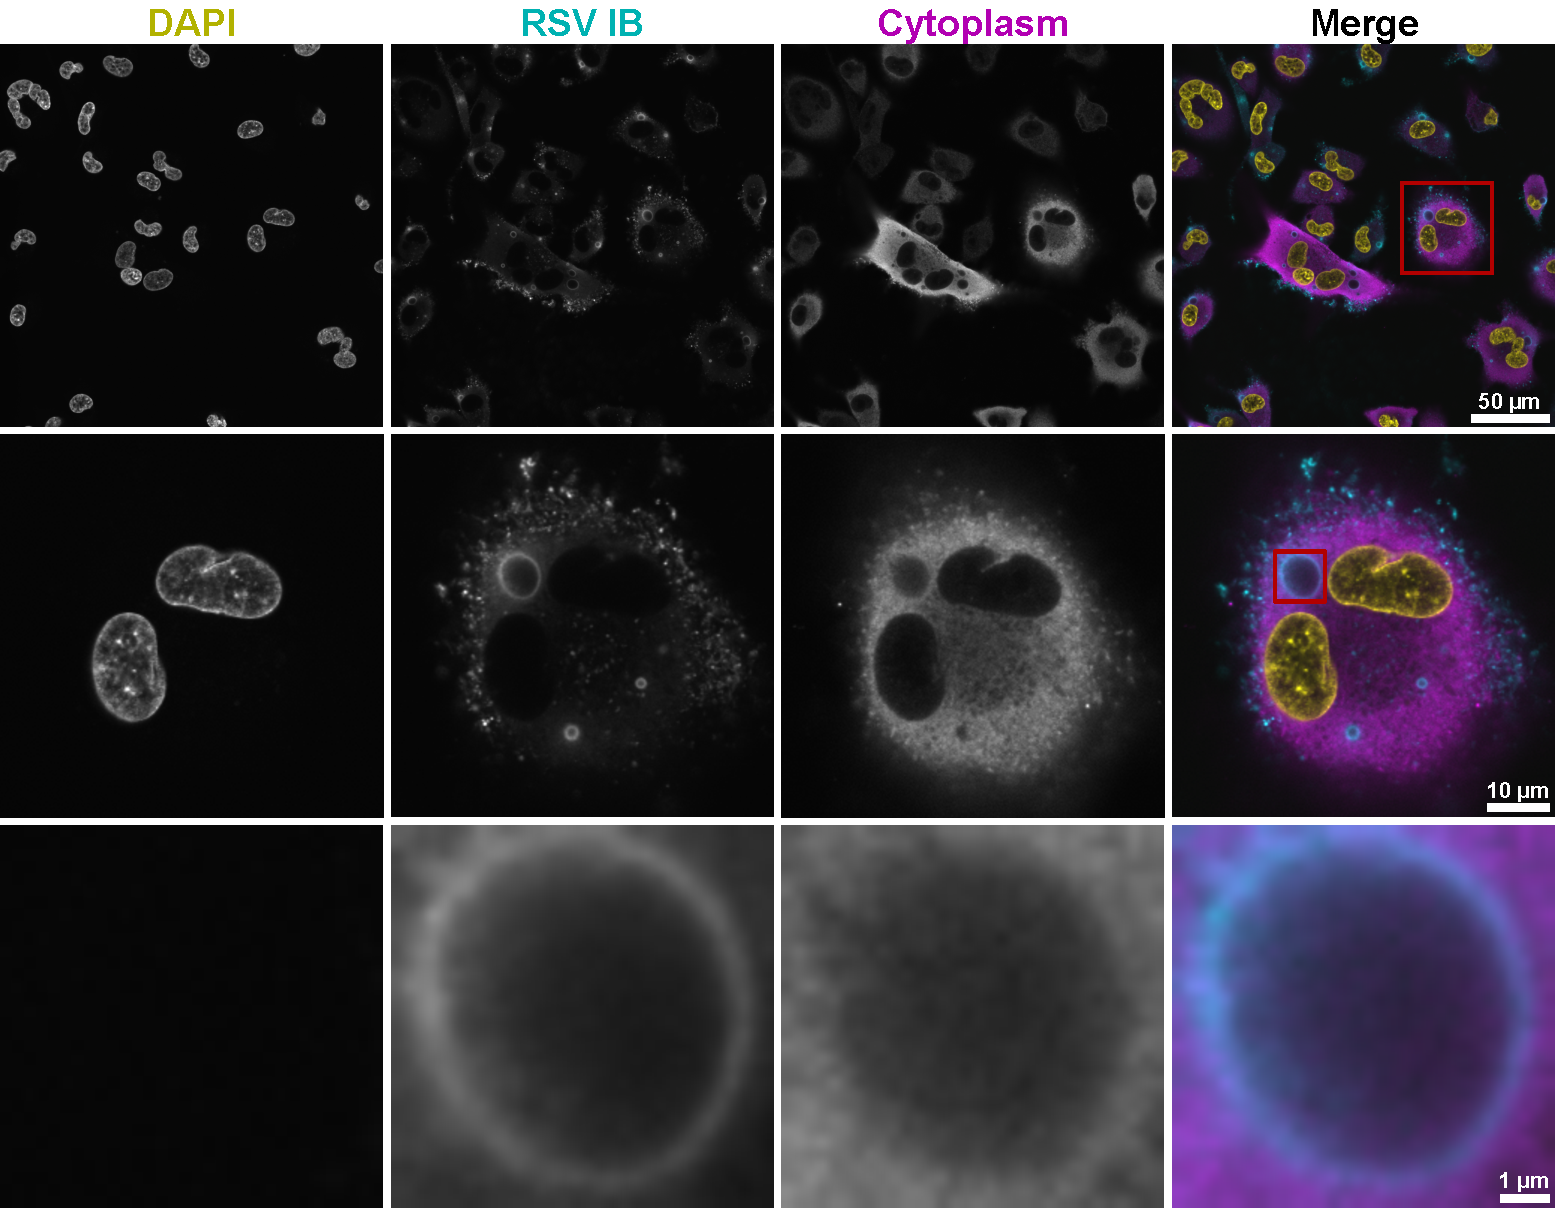
\includegraphics[width=1\linewidth]{08. Chapter 3/Figs/01. Localisation introduction/01. IB-zooms.pdf}
    \caption[Inclusion Bodies Within RSV-Infected Cells: Zoom Sequence.]{\textbf{Inclusion Bodies Within RSV-Infected Cells: Zoom Sequence.} A representative image of RSV-infected cells detected using confocal microscopy. Cellular nuclei were stained with DAPI and are depicted in yellow; RSV inclusion bodies, stained for RSV P, are represented in cyan; and the cytoplasm, stained for IFIT5, is illustrated in magenta. The figure showcases a zoom sequence starting from a population of cells, progressing to a single syncytial view, and ultimately focusing on an individual inclusion body.}
    \label{fig:Inclusion Bodies Within RSV Infected Cells: Zoom Sequence}
\end{figure}

We systematically observed and annotated a total of 1727 inclusion bodies across different cell lines, categorising their IFIT interaction phenotypes and measuring their radii (µm) and areas (\(\mbox{µm}^2\)) based on the observed 2D projections. Specifically, we analysed 1008 hRSV IBs in the A549 cell line, 99 hRSV IBs in the BEAS2B cell line, and 620 bRSV IBs in the MDBK cell line. Figure \ref{fig:Size Characterization of Inclusion Bodies Observed Across Different Cell Lines} illustrates the relationship between IB area and radius, both as an aggregate of all observed IBs and IBs detected per cell line. The data, in both the aggregate and individual cell line view, broadly follows a logarithmic curve, indicating the predominant circular shape of the majority of IBs. However, a deviation from this pattern is noticeable in each cell line, particularly in larger IBs, where the area increases disproportionately with the radius, suggesting a more elongated ellipsoid shape. Most IBs, irrespective of their origin, conform to areas below 10 \(\mbox{µm}^2\). Regarding the most common radii, both BEAS2B and MDBK IBs tend to be below 1 µm, while A549 IBs exhibit a range of the most common radii sizes between 0.5 and 1.5 µm. A more detailed view of the distribution of measured areas per cell line can be observed in Figure \ref{fig:The Distributions of IB Areas Observed Per Cell Line}. Here, all three cell lines encompass IBs ranging from sub 0.5 \(\mbox{µm}^2\) to supra 30 \(\mbox{µm}^2\), with median sizes of 5 \(\mbox{µm}^2\), 3 \(\mbox{µm}^2\), and 2 \(\mbox{µm}^2\) for A549, BEAS2B, and MDBK, respectively. MDBK has the highest number of sub 1 \(\mbox{µm}^2\) IBs, while A549 exhibits the most supra 10 \(\mbox{µm}^2\) IBs.

\begin{figure}
    \begin{subfigure}{0.495\textwidth}
        \caption{}
        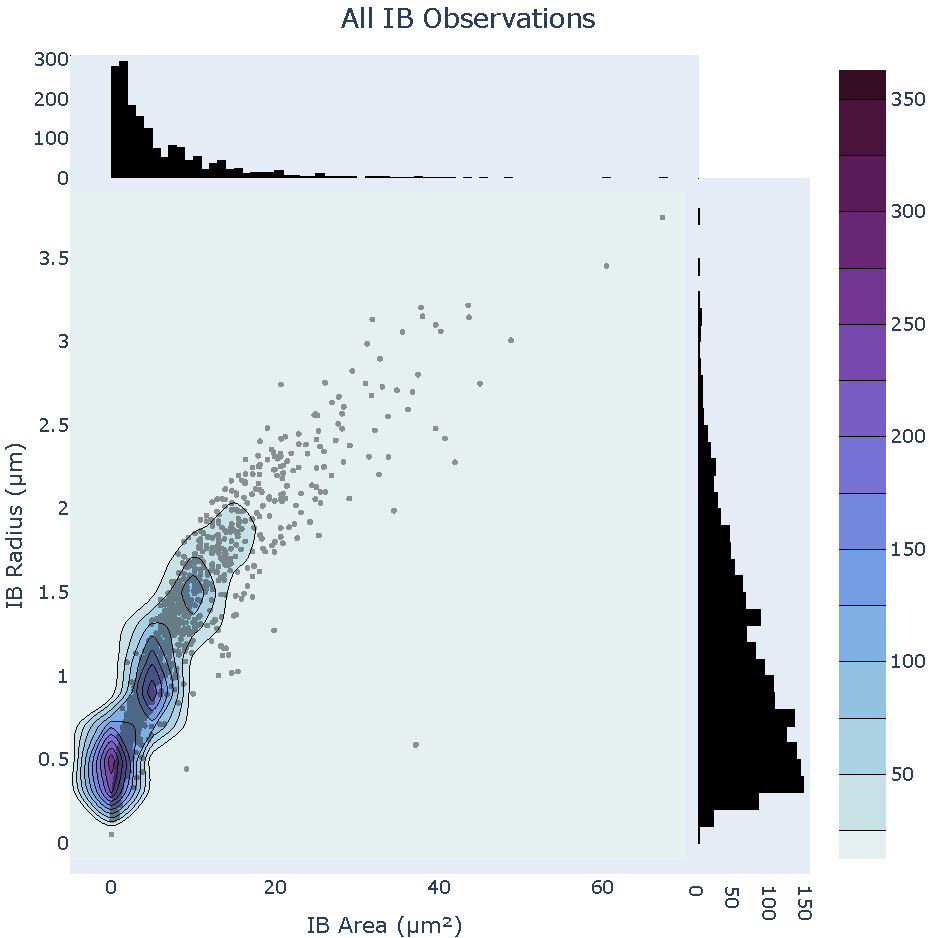
\includegraphics[width=\textwidth]{08. Chapter 3/Figs/01. Localisation introduction/02. heatmap_all.pdf} 
    \end{subfigure}
    \hfill
    \begin{subfigure}{0.495\textwidth}
        \caption{}
        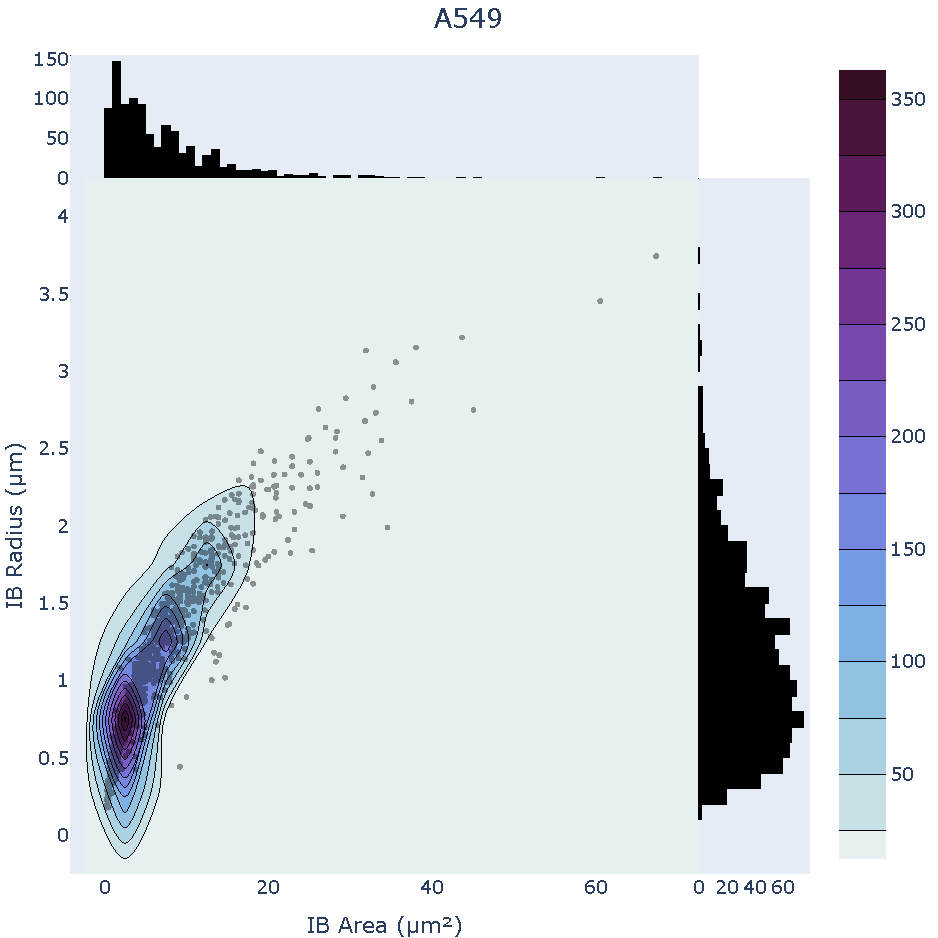
\includegraphics[width=\textwidth]{08. Chapter 3/Figs/01. Localisation introduction/03. heatmap_a549.pdf}
    \end{subfigure}

    \medskip
    \begin{subfigure}{0.495\textwidth}
        \caption{}
        \includegraphics[width=\textwidth]{08. Chapter 3/Figs/01. Localisation introduction/04. heatmap_beas2b.pdf} 
    \end{subfigure}
    \hfill
    \begin{subfigure}{0.495\textwidth}
        \caption{}
        \includegraphics[width=\textwidth]{08. Chapter 3/Figs/01. Localisation introduction/05. heatmap_mdbk.pdf} 
    \end{subfigure}
    \caption[Size Characterisation of Inclusion Bodies Observed Across Different Cell Lines.]{\textbf{Size Characterisation of Inclusion Bodies Observed Across Different Cell Lines.} This figure elucidates the relationship between the measured area (\(\mbox{µm}^2\)) and radius (µm) of individual RSV inclusion bodies observed in this study. The figure includes distinct population distributions alongside the plots: (a) an aggregate of 1727 IB observations across all cell lines, (b) 1008 observations from the A549 cell line, (c) 99 observations from the BEAS2B cell line, and (d) 620 observations from the MDBK cell line. Contour plots are incorporated to highlight the density of individual IBs within the plots.}
    \label{fig:Size Characterization of Inclusion Bodies Observed Across Different Cell Lines}
\end{figure}

From the published literature, it is established that an increase in IB area correlates with its maturation state and internal complexity. Notably, in the HEp-2 cell line infected with hRSV, it has been reported that IBs containing IBAGs are significantly larger than those without (6.4 \(\mbox{µm}^2\) versus 2.3 \(\mbox{µm}^2\)) \cite{Rincheval2017FunctionalVirus}. Additionally, in the MDBK cell line, during the early infection timepoint (6 hours post-infection), only small IBs are present, with a mean area value of 1 \(\mbox{µm}^2\), and these do not contain IBAGs. At 16 hours post-infection, IBs without IBAGs retain the mean area value, while larger IBs with IBAGs (mean area of 10 \(\mbox{µm}^2\)) are also observed \cite{Jobe2021BovineResponses}. Importantly, at 24 HPI, a critical timepoint for the analysis in this thesis, small IBs without IBAGs maintain a median size of 1 \(\mbox{µm}^2\), while larger IBs containing IBAGs cluster into two sizes, with mean areas of 2.5 \(\mbox{µm}^2\) and 17 \(\mbox{µm}^2\). Based on this information, we can assess the observed IFIT-IB interaction phenotypes per mature or immature IBs.

\begin{figure}
    \centering
    \includegraphics[width=1\linewidth]{08. Chapter 3/Figs/01. Localisation introduction/06. box-infection.pdf}
    \caption[The Distributions of IB Areas Observed per Cell Line.]{\textbf{The Distributions of IB Areas Observed per Cell Line.} The distribution of RSV inclusion body areas (\(\mbox{µm}^2\)), detected in this study are shown. A total of 1008 observations were made in the A549 cell line, 99 observations in the BEAS2B cell line, and 620 observations in the MDBK cell line.}
    \label{fig:The Distributions of IB Areas Observed Per Cell Line}
\end{figure}
\subsection{Nascent Human and Bovine IFIT Localisation During RSV Infection} \label{subsec:Nascent Human and Bovine IFIT Localisation During RSV Infection}
\subsubsection{Phenotypic Diversity of Nascent IFIT1 Interaction with RSV Inclusion Bodies}
following a hint of interaction with ibs for some ifits, we went to systematically assess the interaction of all ifits

ifit one, although being predominantly excluded or duffuesd through ibs (suggesting no interaction), is often observed to interact with these structures

inclusion and coloc + eclusion happens in larger ibs (probs more mature), suggesting temporal nature of ifit one interaction

30 excl 30 diff 18 incl 9 coloc + excl 9 edge excl
5, 4.4, 8, 12, 7

\lipsum[1-30]
\begin{figure}
    \begin{subfigure}{0.495\textwidth}
        \caption{}
        \includegraphics[width=1\linewidth]{08. Chapter 3/Figs/02. Infection/01. IFIT1/01. bar_i1_a549.pdf} 
    \end{subfigure}
    \begin{subfigure}{0.495\textwidth}
        \caption{}
        \includegraphics[width=1\linewidth]{08. Chapter 3/Figs/02. Infection/01. IFIT1/02. box_i1_a549.pdf}
    \end{subfigure}
    \caption[Phenotypic Diversity of hIFIT1 Interactions with hRSV Inclusion Bodies in A549 Cell Line.]{\textbf{Phenotypic Diversity of hIFIT1 Interactions with hRSV Inclusion Bodies in A549 Cell Line.} A549 cells were infected with human RSV at MOI 1 and fixed 24 HPI. Cells were double-labeled with with anti-RSV N and anti-IFIT1 antibodies and imaged on confocal microscope. Panel (a) shows percentual proportions of observed phenotypes between hRSV inclusion bodies and hIFIT1 (281 observations), with the red dotted line denoting the 5\% threshold, marking phenotypes considered relevant above this limit. Panel (b) shows the IB area in \(\mu m^2\) per observed relevant phenotype.}
    \label{fig:Phenotypic Diversity of hIFIT1 Interactions with hRSV Inclusion Bodies in A549 Cell Line}
\end{figure}

\begin{figure}
    \centering
    \includegraphics[width=1\linewidth]{08. Chapter 3/Figs/02. Infection/01. IFIT1/03. a549 i1.pdf}
    \caption[Representative Images of Phenotypic Diversity of hIFIT1 Interactions with hRSV Inclusion Bodies in A549 Cell Line.]{\textbf{Representative Images of Phenotypic Diversity of hIFIT1 Interactions with hRSV Inclusion Bodies in A549 Cell Line.} A549 cells were infected with hRSV at MOI 1 and fixed at 24 HPI. Cellular nuclei were stained with DAPI (yellow), and cells were double-labeled with anti-RSV N (cyan) and anti-IFIT1 (magenta) antibodies. This figure showcases representative examples of relevant phenotypes in the interaction between hIFIT1 and hRSV inclusion bodies. These phenotypes are presented in descending order based on their percentage proportions. The scale bar indicates 2 \(\mu m\).}
    \label{fig:Representative Images of Phenotypic Diversity of hIFIT1 Interactions with hRSV Inclusion Bodies in A549 Cell Line}
\end{figure}

in beas2bs there is mainly exclsion 86\% with some diffusion 8\%.

diffusion happens in smaller ibs 0.5 (compared to 3)

\begin{figure}
    \begin{subfigure}{0.495\textwidth}
        \caption{}
        \includegraphics[width=1\linewidth]{08. Chapter 3/Figs/02. Infection/01. IFIT1/04. bar_i1_beas2b.pdf} 
    \end{subfigure}
    \begin{subfigure}{0.495\textwidth}
        \caption{}
        \includegraphics[width=1\linewidth]{08. Chapter 3/Figs/02. Infection/01. IFIT1/05. box_i1_beas2b.pdf}
    \end{subfigure}
    \caption[Phenotypic Diversity of hIFIT1 Interactions with hRSV Inclusion Bodies in BEAS2B Cell Line.]{\textbf{Phenotypic Diversity of hIFIT1 Interactions with hRSV Inclusion Bodies in BEAS2B Cell Line.} BEAS2B cells were infected with human RSV at MOI 1 and fixed 24 HPI. Cells were double-labeled with with anti-RSV N and anti-IFIT1 antibodies and imaged on confocal microscope. Panel (a) shows percentual proportions of observed phenotypes between hRSV inclusion bodies and hIFIT1 (281 observations), with the red dotted line denoting the 5\% threshold, marking phenotypes considered relevant above this limit. Panel (b) shows the IB area in \(\mu m^2\) per observed relevant phenotype.}
    \label{fig:Phenotypic Diversity of hIFIT1 Interactions with hRSV Inclusion Bodies in BEAS2B Cell Line}
\end{figure}

\begin{figure}
    \centering
    \includegraphics[width=1\linewidth]{08. Chapter 3/Figs/02. Infection/01. IFIT1/06. beas2b i1.pdf}
    \caption[Representative Images of Phenotypic Diversity of hIFIT1 Interactions with hRSV Inclusion Bodies in BEAS2B Cell Line.]{\textbf{Representative Images of Phenotypic Diversity of hIFIT1 Interactions with hRSV Inclusion Bodies in BEAS2B Cell Line.} BEAS2B cells were infected with hRSV at MOI 1 and fixed at 24 HPI. Cellular nuclei were stained with DAPI (yellow), and cells were double-labeled with anti-RSV N (cyan) and anti-IFIT1 (magenta) antibodies. This figure showcases representative examples of relevant phenotypes in the interaction between hIFIT1 and hRSV inclusion bodies. These phenotypes are presented in descending order based on their percentage proportions. The scale bar indicates 2 \(\mu m\).}
    \label{fig:Representative Images of Phenotypic Diversity of hIFIT1 Interactions with hRSV Inclusion Bodies in BEAS2B Cell Line}
\end{figure}

66 excl, 23 incl, 5 diff

2, 1, 1.5

\begin{figure}
    \begin{subfigure}{0.495\textwidth}
        \caption{}
        \includegraphics[width=1\linewidth]{08. Chapter 3/Figs/02. Infection/01. IFIT1/07. bar_i1_mdbk.pdf} 
    \end{subfigure}
    \begin{subfigure}{0.495\textwidth}
        \caption{}
        \includegraphics[width=1\linewidth]{08. Chapter 3/Figs/02. Infection/01. IFIT1/08. box_i1_mdbk.pdf}
    \end{subfigure}
    \caption[Phenotypic Diversity of bIFIT1 Interactions with bRSV Inclusion Bodies in MDBK Cell Line.]{\textbf{Phenotypic Diversity of bIFIT1 Interactions with bRSV Inclusion Bodies in MDBK Cell Line.} MDBK cells were infected with bovine RSV at MOI 1 and fixed 24 HPI. Cells were double-labeled with with anti-RSV N and anti-IFIT1 antibodies and imaged on confocal microscope. Panel (a) shows percentual proportions of observed phenotypes between bRSV inclusion bodies and bIFIT1 (117 observations), with the red dotted line denoting the 5\% threshold, marking phenotypes considered relevant above this limit. Panel (b) shows the IB area in \(\mu m^2\) per observed relevant phenotype.}
    \label{fig:Phenotypic Diversity of bIFIT1 Interactions with bRSV Inclusion Bodies in MDBK Cell Line}
\end{figure}

\begin{figure}
    \centering
    \includegraphics[width=1\linewidth]{08. Chapter 3/Figs/02. Infection/01. IFIT1/09. mdbk i1.pdf}
    \caption[Representative Images of Phenotypic Diversity of bIFIT1 Interactions with bRSV Inclusion Bodies in MDBK Cell Line.]{\textbf{Representative Images of Phenotypic Diversity of bIFIT1 Interactions with bRSV Inclusion Bodies in MDBK Cell Line.} MDBK cells were infected with bRSV at MOI 1 and fixed at 24 HPI. Cellular nuclei were stained with DAPI (yellow), and cells were double-labeled with anti-RSV N (cyan) and anti-IFIT1 (magenta) antibodies. This figure showcases representative examples of relevant phenotypes in the interaction between bIFIT1 and bRSV inclusion bodies. These phenotypes are presented in descending order based on their percentage proportions. The scale bar indicates 2 \(\mu m\).}
    \label{fig:Representative Images of Phenotypic Diversity of bIFIT1 Interactions with bRSV Inclusion Bodies in MDBK Cell Line}
\end{figure}

\subsubsection{Phenotypic Diversity of Nascent IFIT2 Interaction with RSV Inclusion Bodies}

\begin{figure}
    \begin{subfigure}{0.495\textwidth}
        \caption{}
        \includegraphics[width=1\linewidth]{08. Chapter 3/Figs/02. Infection/02. IFIT2/01. IFIT2A/01. bar_i2a_a549-n.pdf}
    \end{subfigure}
    \begin{subfigure}{0.495\textwidth}
        \caption{}
        \includegraphics[width=1\linewidth]{08. Chapter 3/Figs/02. Infection/02. IFIT2/01. IFIT2A/02. box_i2a_a549-n.pdf}
    \end{subfigure}
    \caption[Phenotypic Diversity of hIFIT2 Interactions with Nucleoprotein-Stained hRSV Inclusion Bodies, Detected by IFIT2A Antibody in A549 Cell Line.]{\textbf{Phenotypic Diversity of hIFIT2 Interactions with Nucleoprotein-Stained hRSV Inclusion Bodies, Detected by IFIT2A Antibody in A549 Cell Line.} A549 cells were infected with human RSV at MOI 1 and fixed 24 HPI. Cells were labeled with anti-RSV N and anti-IFIT2A antibodies and imaged on confocal microscope. Panel (a) shows percentual proportions of observed phenotypes between hRSV inclusion bodies and hIFIT2, detected by IFIT2A antibody (47 observations), with the red dotted line denoting the 5\% threshold, marking phenotypes considered relevant above this limit. Panel (b) shows the IB area in \(\mu m^2\) per observed relevant phenotype.}
    \label{fig:Phenotypic Diversity of hIFIT2 Interactions with Nucleoprotein-Stained hRSV Inclusion Bodies, Detected by IFIT2A Antibody in A549 Cell Line}
\end{figure}

\begin{figure}
    \centering
    \includegraphics[width=1\linewidth]{08. Chapter 3/Figs/02. Infection/02. IFIT2/01. IFIT2A/03. i2a a549 hrsv n.pdf}
    \caption[Representative Images of Phenotypic Diversity of hIFIT2 Interactions with Nucleoprotein-Stained hRSV Inclusion Bodies, Detected by IFIT2A Antibody in A549 Cell Line.]{\textbf{Representative Images of Phenotypic Diversity of hIFIT2 Interactions with Nucleoprotein-Stained hRSV Inclusion Bodies, Detected by IFIT2A Antibody in A549 Cell Line.} A549 cells were infected with hRSV at MOI 1 and fixed at 24 HPI. Cellular nuclei were stained with DAPI (yellow), and cells were double-labeled with anti-RSV N (cyan) and anti-IFIT2A (magenta) antibodies. This figure showcases representative examples of relevant phenotypes in the interaction between hIFIT2, detected by IFIT2A antibody, and hRSV inclusion bodies. These phenotypes are presented in descending order based on their percentage proportions. The scale bar indicates 2 \(\mu m\).}
    \label{fig:Representative Images of Phenotypic Diversity of hIFIT2 Interactions with Nucleoprotein-Stained hRSV Inclusion Bodies, Detected by IFIT2A Antibody in A549 Cell Line}
\end{figure}

60 30 8

3 12 2.6

Nascent human IFIT2 colocalises with the ring structure (outlined by RSV P staining) and to the inner edge of the IB.

\begin{figure}
    \begin{subfigure}{0.495\textwidth}
        \caption{}
        \includegraphics[width=1\linewidth]{08. Chapter 3/Figs/02. Infection/02. IFIT2/01. IFIT2A/04. bar_i2a_a549-p.pdf} 
    \end{subfigure}
    \begin{subfigure}{0.495\textwidth}
        \caption{}
        \includegraphics[width=1\linewidth]{08. Chapter 3/Figs/02. Infection/02. IFIT2/01. IFIT2A/05. box_i2a_a549-p.pdf}
    \end{subfigure}
    \caption[Phenotypic Diversity of hIFIT2 Interactions with Phosphoprotein-Stained hRSV Inclusion Bodies, Detected by IFIT2A Antibody in A549 Cell Line.]{\textbf{Phenotypic Diversity of hIFIT2 Interactions with Phosphoprotein-Stained hRSV Inclusion Bodies, Detected by IFIT2A Antibody in A549 Cell Line.} A549 cells were infected with human RSV at MOI 1 and fixed 24 HPI. Cells were labeled with anti-RSV P and anti-IFIT2A antibodies and imaged on confocal microscope. Panel (a) shows percentual proportions of observed phenotypes between hRSV inclusion bodies and hIFIT2, detected by IFIT2A antibody (48 observations), with the red dotted line denoting the 5\% threshold, marking phenotypes considered relevant above this limit. Panel (b) shows the IB area in \(\mu m^2\) per observed relevant phenotype.}
    \label{fig:Phenotypic Diversity of hIFIT2 Interactions with Phosphoprotein-Stained hRSV Inclusion Bodies, Detected by IFIT2A Antibody in A549 Cell Line}
\end{figure}

\begin{figure}
    \centering
    \includegraphics[width=1\linewidth]{08. Chapter 3/Figs/02. Infection/02. IFIT2/01. IFIT2A/06. i2a a549 hrsv p.pdf} 
    \caption[Representative Images of Phenotypic Diversity of hIFIT2 Interactions with Phosphoprotein-Stained hRSV Inclusion Bodies, Detected by IFIT2A Antibody in A549 Cell Line.]{\textbf{Representative Images of Phenotypic Diversity of hIFIT2 Interactions with Phosphoprotein-Stained hRSV Inclusion Bodies, Detected by IFIT2A Antibody in A549 Cell Line.} A549 cells were infected with hRSV at MOI 1 and fixed at 24 HPI. Cellular nuclei were stained with DAPI (yellow), and cells were double-labeled with anti-RSV P (cyan) and anti-IFIT2A (magenta) antibodies. This figure showcases representative examples of relevant phenotypes in the interaction between hIFIT2, detected by IFIT2A antibody, and hRSV inclusion bodies. These phenotypes are presented in descending order based on their percentage proportions. The scale bar indicates 2 \(\mu m\).}
    \label{fig:Representative Images of Phenotypic Diversity of hIFIT2 Interactions with Phosphoprotein-Stained hRSV Inclusion Bodies, Detected by IFIT2A Antibody in A549 Cell Line}
\end{figure}

82 18

2.5 7.3

With regards of colocalization with human RSV M2/1 protein, human IFIT2 seems to either form inclusion, which has a signal decrease towards the middle of the IB structure (top panel), or seems to strongly colocalise with the ring structure highlighted by M2/1 staining (bottom 2 panels; there also seems to be IFIT2 signal concentration on the inner edge of the IB structure).

\begin{figure}
    \begin{subfigure}{0.495\textwidth}
        \caption{}
        \includegraphics[width=1\linewidth]{08. Chapter 3/Figs/02. Infection/02. IFIT2/01. IFIT2A/07. bar_i2a_a549-m21.pdf} 
    \end{subfigure}
    \begin{subfigure}{0.495\textwidth}
        \caption{}
        \includegraphics[width=1\linewidth]{08. Chapter 3/Figs/02. Infection/02. IFIT2/01. IFIT2A/08. box_i2a_a549-m21.pdf}
    \end{subfigure}
    \caption[Phenotypic Diversity of hIFIT2 Interactions with M2/1-Stained hRSV Inclusion Bodies, Detected by IFIT2A Antibody in A549 Cell Line.]{\textbf{Phenotypic Diversity of hIFIT2 Interactions with M2/1-Stained hRSV Inclusion Bodies, Detected by IFIT2A Antibody in A549 Cell Line.} A549 cells were infected with human RSV at MOI 1 and fixed 24 HPI. Cells were labeled with anti-RSV M2/1 and anti-IFIT2A antibodies and imaged on confocal microscope. Panel (a) shows percentual proportions of observed phenotypes between hRSV inclusion bodies and hIFIT2, detected by IFIT2A antibody (69 observations), with the red dotted line denoting the 5\% threshold, marking phenotypes considered relevant above this limit. Panel (b) shows the IB area in \(\mu m^2\) per observed relevant phenotype.}
    \label{fig:Phenotypic Diversity of hIFIT2 Interactions with M2/1-Stained hRSV Inclusion Bodies, Detected by IFIT2A Antibody in A549 Cell Line}
\end{figure}

\begin{figure}
    \centering
    \includegraphics[width=1\linewidth]{08. Chapter 3/Figs/02. Infection/02. IFIT2/01. IFIT2A/09. i2a a549 hrsv m21.pdf} 
    \caption[Representative Images of Phenotypic Diversity of hIFIT2 Interactions with M2/1-Stained hRSV Inclusion Bodies, Detected by IFIT2A Antibody in A549 Cell Line.]{\textbf{Representative Images of Phenotypic Diversity of hIFIT2 Interactions with M2/1-Stained hRSV Inclusion Bodies, Detected by IFIT2A Antibody in A549 Cell Line.} A549 cells were infected with hRSV at MOI 1 and fixed at 24 HPI. Cellular nuclei were stained with DAPI (yellow), and cells were double-labeled with anti-RSV M2/1 (cyan) and anti-IFIT2A (magenta) antibodies. This figure showcases representative examples of relevant phenotypes in the interaction between hIFIT2, detected by IFIT2A antibody, and hRSV inclusion bodies. These phenotypes are presented in descending order based on their percentage proportions. The scale bar indicates 2 \(\mu m\).}
    \label{fig:Representative Images of Phenotypic Diversity of hIFIT2 Interactions with M2/1-Stained hRSV Inclusion Bodies, Detected by IFIT2A Antibody in A549 Cell Line}
\end{figure}

81 19

1 10

\begin{figure}
    \begin{subfigure}{0.495\textwidth}
        \caption{}
        \includegraphics[width=1\linewidth]{08. Chapter 3/Figs/02. Infection/02. IFIT2/02. IFIT2B/01. bar_i2b_a549-n.pdf}
    \end{subfigure}
    \begin{subfigure}{0.495\textwidth}
        \caption{}
        \includegraphics[width=1\linewidth]{08. Chapter 3/Figs/02. Infection/02. IFIT2/02. IFIT2B/02. box_i2b_a549-n.pdf}
    \end{subfigure}
    \caption[Phenotypic Diversity of hIFIT2 Interactions with Nucleoprotein-Stained hRSV Inclusion Bodies, Detected by IFIT2B Antibody in A549 Cell Line.]{\textbf{Phenotypic Diversity of hIFIT2 Interactions with Nucleoprotein-Stained hRSV Inclusion Bodies, Detected by IFIT2B Antibody in A549 Cell Line.} A549 cells were infected with human RSV at MOI 1 and fixed 24 HPI. Cells were labeled with anti-RSV N and anti-IFIT2B antibodies and imaged on confocal microscope. Panel (a) shows percentual proportions of observed phenotypes between hRSV inclusion bodies and hIFIT2, detected by IFIT2B antibody (56 observations), with the red dotted line denoting the 5\% threshold, marking phenotypes considered relevant above this limit. Panel (b) shows the IB area in \(\mu m^2\) per observed relevant phenotype.}
    \label{fig:Phenotypic Diversity of hIFIT2 Interactions with Nucleoprotein-Stained hRSV Inclusion Bodies, Detected by IFIT2B Antibody in A549 Cell Line}
\end{figure}

\begin{figure}
    \centering
    \includegraphics[width=1\linewidth]{08. Chapter 3/Figs/02. Infection/02. IFIT2/02. IFIT2B/03. i2b a549 hrsv n.pdf} 
    \caption[Representative Images of Phenotypic Diversity of hIFIT2 Interactions with Nucleoprotein-Stained hRSV Inclusion Bodies, Detected by IFIT2B Antibody in A549 Cell Line.]{\textbf{Representative Images of Phenotypic Diversity of hIFIT2 Interactions with Nucleoprotein-Stained hRSV Inclusion Bodies, Detected by IFIT2B Antibody in A549 Cell Line.} A549 cells were infected with hRSV at MOI 1 and fixed at 24 HPI. Cellular nuclei were stained with DAPI (yellow), and cells were double-labeled with anti-RSV N (cyan) and anti-IFIT2B (magenta) antibodies. This figure showcases representative examples of relevant phenotypes in the interaction between hIFIT2, detected by IFIT2B antibody, and hRSV inclusion bodies. These phenotypes are presented in descending order based on their percentage proportions. The scale bar indicates 2 \(\mu m\).}
    \label{fig:Representative Images of Phenotypic Diversity of hIFIT2 Interactions with Nucleoprotein-Stained hRSV Inclusion Bodies, Detected by IFIT2B Antibody in A549 Cell Line}
\end{figure}

96

2.1

Endogenous human IFIT2 is either partially excluded (top panel; decrease of intra IB signal compared to cytoplasmic signal) or completely excluded (bottom panel) from the human IB structure.

\begin{figure}
    \begin{subfigure}{0.495\textwidth}
        \caption{}
        \includegraphics[width=1\linewidth]{08. Chapter 3/Figs/02. Infection/02. IFIT2/02. IFIT2B/04. bar_i2b_a549-p.pdf} 
    \end{subfigure}
    \begin{subfigure}{0.495\textwidth}
        \caption{}
        \includegraphics[width=1\linewidth]{08. Chapter 3/Figs/02. Infection/02. IFIT2/02. IFIT2B/05. box_i2b_a549-p.pdf}
    \end{subfigure}
    \caption[Phenotypic Diversity of hIFIT2 Interactions with Phosphoprotein-Stained hRSV Inclusion Bodies, Detected by IFIT2B Antibody in A549 Cell Line.]{\textbf{Phenotypic Diversity of hIFIT2 Interactions with Phosphoprotein-Stained hRSV Inclusion Bodies, Detected by IFIT2B Antibody in A549 Cell Line.} A549 cells were infected with human RSV at MOI 1 and fixed 24 HPI. Cells were labeled with anti-RSV P and anti-IFIT2B antibodies and imaged on confocal microscope. Panel (a) shows percentual proportions of observed phenotypes between hRSV inclusion bodies and hIFIT2, detected by IFIT2B antibody (27 observations), with the red dotted line denoting the 5\% threshold, marking phenotypes considered relevant above this limit. Panel (b) shows the IB area in \(\mu m^2\) per observed relevant phenotype.}
    \label{fig:Phenotypic Diversity of hIFIT2 Interactions with Phosphoprotein-Stained hRSV Inclusion Bodies, Detected by IFIT2B Antibody in A549 Cell Line}
\end{figure}

\begin{figure}
    \centering
    \includegraphics[width=1\linewidth]{08. Chapter 3/Figs/02. Infection/02. IFIT2/02. IFIT2B/06. i2b a549 hrsv p.pdf} 
    \caption[Representative Images of Phenotypic Diversity of hIFIT2 Interactions with Phosphoprotein-Stained hRSV Inclusion Bodies, Detected by IFIT2B Antibody in A549 Cell Line.]{\textbf{Representative Images of Phenotypic Diversity of hIFIT2 Interactions with Phosphoprotein-Stained hRSV Inclusion Bodies, Detected by IFIT2B Antibody in A549 Cell Line.} A549 cells were infected with hRSV at MOI 1 and fixed at 24 HPI. Cellular nuclei were stained with DAPI (yellow), and cells were double-labeled with anti-RSV P (cyan) and anti-IFIT2B (magenta) antibodies. This figure showcases representative examples of relevant phenotypes in the interaction between hIFIT2, detected by IFIT2B antibody, and hRSV inclusion bodies. These phenotypes are presented in descending order based on their percentage proportions. The scale bar indicates 2 \(\mu m\).}
    \label{fig:Representative Images of Phenotypic Diversity of hIFIT2 Interactions with Phosphoprotein-Stained hRSV Inclusion Bodies, Detected by IFIT2B Antibody in A549 Cell Line}
\end{figure}

78 22

4.3 1.3

We observe similar pattern of staining to what was observed with N stained human IBs. IFIT2 signal is either partially or totally excluded from the IB structure.

\begin{figure}
    \begin{subfigure}{0.495\textwidth}
        \caption{}
        \includegraphics[width=1\linewidth]{08. Chapter 3/Figs/02. Infection/02. IFIT2/02. IFIT2B/07. bar_i2b_a549-m21.pdf} 
    \end{subfigure}
    \begin{subfigure}{0.495\textwidth}
        \caption{}
        \includegraphics[width=1\linewidth]{08. Chapter 3/Figs/02. Infection/02. IFIT2/02. IFIT2B/08. box_i2b_a549-m21.pdf}
    \end{subfigure}
    \caption[Phenotypic Diversity of hIFIT2 Interactions with M2/1-Stained hRSV Inclusion Bodies, Detected by IFIT2B Antibody in A549 Cell Line.]{\textbf{Phenotypic Diversity of hIFIT2 Interactions with M2/1-Stained hRSV Inclusion Bodies, Detected by IFIT2B Antibody in A549 Cell Line.} A549 cells were infected with human RSV at MOI 1 and fixed 24 HPI. Cells were labeled with anti-RSV M2/1 and anti-IFIT2B antibodies and imaged on confocal microscope. Panel (a) shows percentual proportions of observed phenotypes between hRSV inclusion bodies and hIFIT2, detected by IFIT2B antibody (31 observations), with the red dotted line denoting the 5\% threshold, marking phenotypes considered relevant above this limit. Panel (b) shows the IB area in \(\mu m^2\) per observed relevant phenotype.}
    \label{fig:Phenotypic Diversity of hIFIT2 Interactions with M2/1-Stained hRSV Inclusion Bodies, Detected by IFIT2B Antibody in A549 Cell Line}
\end{figure}

\begin{figure}
    \centering
    \includegraphics[width=1\linewidth]{08. Chapter 3/Figs/02. Infection/02. IFIT2/02. IFIT2B/09. i2b a549 hrsv m21.pdf} 
    \caption[Representative Images of Phenotypic Diversity of hIFIT2 Interactions with M2/1-Stained hRSV Inclusion Bodies, Detected by IFIT2B Antibody in A549 Cell Line.]{\textbf{Representative Images of Phenotypic Diversity of hIFIT2 Interactions with M2/1-Stained hRSV Inclusion Bodies, Detected by IFIT2B Antibody in A549 Cell Line.} A549 cells were infected with hRSV at MOI 1 and fixed at 24 HPI. Cellular nuclei were stained with DAPI (yellow), and cells were double-labeled with anti-RSV M2/1 (cyan) and anti-IFIT2B (magenta) antibodies. This figure showcases representative examples of relevant phenotypes in the interaction between hIFIT2, detected by IFIT2B antibody, and hRSV inclusion bodies. These phenotypes are presented in descending order based on their percentage proportions. The scale bar indicates 2 \(\mu m\).}
    \label{fig:Representative Images of Phenotypic Diversity of hIFIT2 Interactions with M2/1-Stained hRSV Inclusion Bodies, Detected by IFIT2B Antibody in A549 Cell Line}
\end{figure}

71 21 6

2.1 8 15

Endogenous human IFIT2 seems to be excluded from hRSV IBs.

\begin{figure}
    \begin{subfigure}{0.495\textwidth}
        \caption{}
        \includegraphics[width=1\linewidth]{08. Chapter 3/Figs/02. Infection/02. IFIT2/01. IFIT2A/10. bar_i2a_beas2b.pdf} 
    \end{subfigure}
    \begin{subfigure}{0.495\textwidth}
        \caption{}
        \includegraphics[width=1\linewidth]{08. Chapter 3/Figs/02. Infection/02. IFIT2/01. IFIT2A/11. box_i2a_beas2b.pdf}
    \end{subfigure}
    \caption[Phenotypic Diversity of hIFIT2 Interactions with hRSV Inclusion Bodies, Detected by IFIT2A Antibody in BEAS2B Cell Line.]{\textbf{Phenotypic Diversity of hIFIT2 Interactions with hRSV Inclusion Bodies, Detected by IFIT2A Antibody in BEAS2B Cell Line.} BEAS2B cells were infected with human RSV at MOI 1 and fixed 24 HPI. Cells were labeled with anti-RSV N and anti-IFIT2A antibodies and imaged on confocal microscope. Panel (a) shows percentual proportions of observed phenotypes between hRSV inclusion bodies and hIFIT2, detected by IFIT2A antibody (99 observations), with the red dotted line denoting the 5\% threshold, marking phenotypes considered relevant above this limit. Panel (b) shows the IB area in \(\mu m^2\) per observed relevant phenotype.}
    \label{fig:Phenotypic Diversity of hIFIT2 Interactions with hRSV Inclusion Bodies, Detected by IFIT2A Antibody in BEAS2B Cell Line}
\end{figure}

\begin{figure}
    \centering
    \includegraphics[width=1\linewidth]{08. Chapter 3/Figs/02. Infection/02. IFIT2/01. IFIT2A/12. i2a beas2b.pdf} 
    \caption[Representative Images of Phenotypic Diversity of hIFIT2 Interactions with hRSV Inclusion Bodies, Detected by IFIT2A Antibody in BEAS2B Cell Line.]{\textbf{Representative Images of Phenotypic Diversity of hIFIT2 Interactions with hRSV Inclusion Bodies, Detected by IFIT2A Antibody in BEAS2B Cell Line.} BEAS2B cells were infected with hRSV at MOI 1 and fixed at 24 HPI. Cellular nuclei were stained with DAPI (yellow), and cells were double-labeled with anti-RSV N (cyan) and anti-IFIT2A (magenta) antibodies. This figure showcases representative examples of relevant phenotypes in the interaction between hIFIT2, detected by IFIT2A antibody, and hRSV inclusion bodies. These phenotypes are presented in descending order based on their percentage proportions. The scale bar indicates 2 \(\mu m\).}
    \label{fig:Representative Images of Phenotypic Diversity of hIFIT2 Interactions with hRSV Inclusion Bodies, Detected by IFIT2A Antibody in BEAS2B Cell Line}
\end{figure}

58 35 5

3 1.2 1.2


Nascent bovine IFIT2 colocalization with regards of N stained bRSV IBs seems to strongly associate with the ring of the structure.

\begin{figure}
    \begin{subfigure}{0.495\textwidth}
        \caption{}
        \includegraphics[width=1\linewidth]{08. Chapter 3/Figs/02. Infection/02. IFIT2/01. IFIT2A/13. bar_i2a_mdbk.pdf} 
    \end{subfigure}
    \begin{subfigure}{0.495\textwidth}
        \caption{}
        \includegraphics[width=1\linewidth]{08. Chapter 3/Figs/02. Infection/02. IFIT2/01. IFIT2A/14. box_i2a_mdbk.pdf}
    \end{subfigure}
    \caption[Phenotypic Diversity of hIFIT2 Interactions with bRSV Inclusion Bodies, Detected by IFIT2A Antibody in MDBK Cell Line.]{\textbf{Phenotypic Diversity of hIFIT2 Interactions with bRSV Inclusion Bodies, Detected by IFIT2A Antibody in MDBK Cell Line.} MDBK cells were infected with bovine RSV at MOI 1 and fixed 24 HPI. Cells were labeled with anti-RSV N and anti-IFIT2A antibodies and imaged on confocal microscope. Panel (a) shows percentual proportions of observed phenotypes between bRSV inclusion bodies and bIFIT2, detected by IFIT2A antibody (162 observations), with the red dotted line denoting the 5\% threshold, marking phenotypes considered relevant above this limit. Panel (b) shows the IB area in \(\mu m^2\) per observed relevant phenotype.}
    \label{fig:Phenotypic Diversity of hIFIT2 Interactions with bRSV Inclusion Bodies, Detected by IFIT2A Antibody in MDBK Cell Line}
\end{figure}

\begin{figure}
    \centering
    \includegraphics[width=1\linewidth]{08. Chapter 3/Figs/02. Infection/02. IFIT2/01. IFIT2A/15. i2a mdbk brsv.pdf} 
    \caption[Representative Images of Phenotypic Diversity of hIFIT2 Interactions with bRSV Inclusion Bodies, Detected by IFIT2A Antibody in MDBK Cell Line.]{\textbf{Representative Images of Phenotypic Diversity of hIFIT2 Interactions with bRSV Inclusion Bodies, Detected by IFIT2A Antibody in MDBK Cell Line.} MDBK cells were infected with bRSV at MOI 1 and fixed at 24 HPI. Cellular nuclei were stained with DAPI (yellow), and cells were double-labeled with anti-RSV N (cyan) and anti-IFIT2A (magenta) antibodies. This figure showcases representative examples of relevant phenotypes in the interaction between bIFIT2, detected by IFIT2A antibody, and bRSV inclusion bodies. These phenotypes are presented in descending order based on their percentage proportions. The scale bar indicates 2 \(\mu m\).}
    \label{fig:Representative Images of Phenotypic Diversity of hIFIT2 Interactions with bRSV Inclusion Bodies, Detected by IFIT2A Antibody in MDBK Cell Line}
\end{figure}

64 36

1 9

\begin{figure}
    \begin{subfigure}{0.495\textwidth}
        \caption{}
        \includegraphics[width=1\linewidth]{08. Chapter 3/Figs/02. Infection/02. IFIT2/02. IFIT2B/10. bar_i2b_mdbk.pdf} 
    \end{subfigure}
    \begin{subfigure}{0.495\textwidth}
        \caption{}
        \includegraphics[width=1\linewidth]{08. Chapter 3/Figs/02. Infection/02. IFIT2/02. IFIT2B/11. box_i2b_mdbk.pdf}
    \end{subfigure}
    \caption[Phenotypic Diversity of hIFIT2 Interactions with bRSV Inclusion Bodies, Detected by IFIT2B Antibody in MDBK Cell Line.]{\textbf{Phenotypic Diversity of hIFIT2 Interactions with bRSV Inclusion Bodies, Detected by IFIT2B Antibody in MDBK Cell Line.} MDBK cells were infected with bovine RSV at MOI 1 and fixed 24 HPI. Cells were labeled with anti-RSV N and anti-IFIT2B antibodies and imaged on confocal microscope. Panel (a) shows percentual proportions of observed phenotypes between bRSV inclusion bodies and bIFIT2, detected by IFIT2B antibody (66 observations), with the red dotted line denoting the 5\% threshold, marking phenotypes considered relevant above this limit. Panel (b) shows the IB area in \(\mu m^2\) per observed relevant phenotype.}
    \label{fig:Phenotypic Diversity of hIFIT2 Interactions with bRSV Inclusion Bodies, Detected by IFIT2B Antibody in MDBK Cell Line}
\end{figure}

\begin{figure}
    \centering
    \includegraphics[width=1\linewidth]{08. Chapter 3/Figs/02. Infection/02. IFIT2/02. IFIT2B/12. i2b mdbk brsv.pdf} 
    \caption[Representative Images of Phenotypic Diversity of hIFIT2 Interactions with bRSV Inclusion Bodies, Detected by IFIT2B Antibody in MDBK Cell Line.]{\textbf{Representative Images of Phenotypic Diversity of hIFIT2 Interactions with bRSV Inclusion Bodies, Detected by IFIT2B Antibody in MDBK Cell Line.} MDBK cells were infected with bRSV at MOI 1 and fixed at 24 HPI. Cellular nuclei were stained with DAPI (yellow), and cells were double-labeled with anti-RSV N (cyan) and anti-IFIT2B (magenta) antibodies. This figure showcases representative examples of relevant phenotypes in the interaction between bIFIT2, detected by IFIT2B antibody, and bRSV inclusion bodies. These phenotypes are presented in descending order based on their percentage proportions. The scale bar indicates 2 \(\mu m\).}
    \label{fig:Representative Images of Phenotypic Diversity of hIFIT2 Interactions with bRSV Inclusion Bodies, Detected by IFIT2B Antibody in MDBK Cell Line}
\end{figure}

71 21 6

2 8 17

\subsubsection{Phenotypic Diversity of Nascent IFIT3 Interaction with RSV Inclusion Bodies}
Nascent human IFIT3 seems to have mainly diffused phenotype (top and bottom panel) with occasional exclusion without any marked IFIT3 concentration adjacent to the IB structure (middle panel).

53, 17, 16, 10

4.5, 12, 5, 1.9

\begin{figure}
    \begin{subfigure}{0.495\textwidth}
        \caption{}
        \includegraphics[width=1\linewidth]{08. Chapter 3/Figs/02. Infection/03. IFIT3/01. bar_i3_a549.pdf} 
    \end{subfigure}
    \begin{subfigure}{0.495\textwidth}
        \caption{}
        \includegraphics[width=1\linewidth]{08. Chapter 3/Figs/02. Infection/03. IFIT3/02. box_i3_a549.pdf}
    \end{subfigure}
    \caption[Phenotypic Diversity of hIFIT3 Interactions with hRSV Inclusion Bodies in A549 Cell Line.]{\textbf{Phenotypic Diversity of hIFIT3 Interactions with hRSV Inclusion Bodies in A549 Cell Line.} A549 cells were infected with human RSV at MOI 1 and fixed 24 HPI. Cells were double-labeled with with anti-RSV N and anti-IFIT3 antibodies and imaged on confocal microscope. Panel (a) shows percentual proportions of observed phenotypes between hRSV inclusion bodies and hIFIT3 (80 observations), with the red dotted line denoting the 5\% threshold, marking phenotypes considered relevant above this limit. Panel (b) shows the IB area in \(\mu m^2\) per observed relevant phenotype.}
    \label{fig:Phenotypic Diversity of hIFIT3 Interactions with hRSV Inclusion Bodies in A549 Cell Line}
\end{figure}

\begin{figure}
    \centering
    \includegraphics[width=1\linewidth]{08. Chapter 3/Figs/02. Infection/03. IFIT3/03. a549 i3.pdf}
    \caption[Representative Images of Phenotypic Diversity of hIFIT3 Interactions with hRSV Inclusion Bodies in A549 Cell Line.]{\textbf{Representative Images of Phenotypic Diversity of hIFIT3 Interactions with hRSV Inclusion Bodies in A549 Cell Line.} A549 cells were infected with hRSV at MOI 1 and fixed at 24 HPI. Cellular nuclei were stained with DAPI (yellow), and cells were double-labeled with anti-RSV N (cyan) and anti-IFIT3 (magenta) antibodies. This figure showcases representative examples of relevant phenotypes in the interaction between hIFIT3 and hRSV inclusion bodies. These phenotypes are presented in descending order based on their percentage proportions. The scale bar indicates 2 \(\mu m\).}
    \label{fig:Representative Images of Phenotypic Diversity of hIFIT3 Interactions with hRSV Inclusion Bodies in A549 Cell Line}
\end{figure}

62, 19, 12

5.5, 3, 10, 2.3

\begin{figure}
    \begin{subfigure}{0.495\textwidth}
        \caption{}
        \includegraphics[width=1\linewidth]{08. Chapter 3/Figs/02. Infection/03. IFIT3/04. bar_i3_beas2b.pdf} 
    \end{subfigure}
    \begin{subfigure}{0.495\textwidth}
        \caption{}        
        \includegraphics[width=1\linewidth]{08. Chapter 3/Figs/02. Infection/03. IFIT3/05. box_i3_beas2b.pdf}
    \end{subfigure}
    \caption[Phenotypic Diversity of hIFIT3 Interactions with hRSV Inclusion Bodies in BEAS2B Cell Line.]{\textbf{Phenotypic Diversity of hIFIT3 Interactions with hRSV Inclusion Bodies in BEAS2B Cell Line.} BEAS2B cells were infected with human RSV at MOI 1 and fixed 24 HPI. Cells were labeled with anti-RSV N and anti-IFIT3 antibodies and imaged on confocal microscope. Panel (a) shows percentual proportions of observed phenotypes between hRSV inclusion bodies and hIFIT3 (16 observations), with the red dotted line denoting the 5\% threshold, marking phenotypes considered relevant above this limit. Panel (b) shows the IB area in \(\mu m^2\) per observed relevant phenotype.}
    \label{fig:Phenotypic Diversity of hIFIT3 Interactions with hRSV Inclusion Bodies in BEAS2B Cell Line}
\end{figure}

\begin{figure}
    \centering
    \includegraphics[width=1\linewidth]{08. Chapter 3/Figs/02. Infection/03. IFIT3/06. beas2b i3.pdf}
    \caption[Representative Images of Phenotypic Diversity of hIFIT3 Interactions with hRSV Inclusion Bodies in BEAS2B Cell Line]{\textbf{Representative Images of Phenotypic Diversity of hIFIT3 Interactions with hRSV Inclusion Bodies in BEAS2B Cell Line.} BEAS2B cells were infected with hRSV at MOI 1 and fixed at 24 HPI. Cellular nuclei were stained with DAPI (yellow), and cells were double-labeled with anti-RSV N (cyan) and anti-IFIT3 (magenta) antibodies. This figure showcases representative examples of relevant phenotypes in the interaction between hIFIT3 and hRSV inclusion bodies. These phenotypes are presented in descending order based on their percentage proportions. The scale bar indicates 2 \(\mu m\).}
    \label{fig:Representative Images of Phenotypic Diversity of hIFIT3 Interactions with hRSV Inclusion Bodies in BEAS2B Cell Line}
\end{figure}

43, 34, 11, 8

1.1, 3.3, 1, 11

\begin{figure}
    \begin{subfigure}{0.495\textwidth}
        \caption{}
        \includegraphics[width=1\linewidth]{08. Chapter 3/Figs/02. Infection/03. IFIT3/07. bar_i3_mdbk.pdf} 
    \end{subfigure}
    \begin{subfigure}{0.495\textwidth}
        \caption{}
        \includegraphics[width=1\linewidth]{08. Chapter 3/Figs/02. Infection/03. IFIT3/08. box_i3_mdbk.pdf}
    \end{subfigure}
    \caption[Phenotypic Diversity of bIFIT3 Interactions with bRSV Inclusion Bodies in MDBK Cell Line.]{\textbf{Phenotypic Diversity of bIFIT3 Interactions with bRSV Inclusion Bodies in MDBK Cell Line.} MDBK cells were infected with bovine RSV at MOI 1 and fixed 24 HPI. Cells were labeled with anti-RSV N and anti-IFIT3 antibodies and imaged on confocal microscope. Panel (a) shows percentual proportions of observed phenotypes between bRSV inclusion bodies and bIFIT3 (214 observations), with the red dotted line denoting the 5\% threshold, marking phenotypes considered relevant above this limit. Panel (b) shows the IB area in \(\mu m^2\) per observed relevant phenotype.}
    \label{fig:Phenotypic Diversity of bIFIT3 Interactions with bRSV Inclusion Bodies in MDBK Cell Line}
\end{figure}

\begin{figure}
    \centering
    \includegraphics[width=1\linewidth]{08. Chapter 3/Figs/02. Infection/03. IFIT3/09. mdbk i3.pdf}
    \caption[Representative Images of Phenotypic Diversity of bIFIT3 Interactions with bRSV Inclusion Bodies in MDBK Cell Line.]{\textbf{Representative Images of Phenotypic Diversity of bIFIT3 Interactions with bRSV Inclusion Bodies in MDBK Cell Line.} MDBK cells were infected with bRSV at MOI 1 and fixed at 24 HPI. Cellular nuclei were stained with DAPI (yellow), and cells were double-labeled with anti-RSV N (cyan) and anti-IFIT3 (magenta) antibodies. This figure showcases representative examples of relevant phenotypes in the interaction between bIFIT3 and bRSV inclusion bodies. These phenotypes are presented in descending order based on their percentage proportions. The scale bar indicates 2 \(\mu m\).}
    \label{fig:Representative Images of Phenotypic Diversity of bIFIT3 Interactions with bRSV Inclusion Bodies in MDBK Cell Line}
\end{figure}

\subsubsection{Phenotypic Diversity of Nascent IFIT5 Interaction with RSV Inclusion Bodies}
hIFIT5 seems to be excluded from hRSV IBs. There is a hint of accumulation of IFIT5 on the outside of IB (bottom panel; no z stacks to confirm this). 

58, 17, 16, 5

6.3, 4, 8, 13

\begin{figure}
    \begin{subfigure}{0.495\textwidth}
        \caption{}
        \includegraphics[width=1\linewidth]{08. Chapter 3/Figs/02. Infection/04. IFIT5/01. bar_i5_a549.pdf} 
    \end{subfigure}
    \begin{subfigure}{0.495\textwidth}
        \caption{}
        \includegraphics[width=1\linewidth]{08. Chapter 3/Figs/02. Infection/04. IFIT5/02. box_i5_a549.pdf}
    \end{subfigure}
    \caption[Phenotypic Diversity of hIFIT5 Interactions with hRSV Inclusion Bodies in A549 Cell Line.]{\textbf{Phenotypic Diversity of hIFIT5 Interactions with hRSV Inclusion Bodies in A549 Cell Line.} A549 cells were infected with human RSV at MOI 1 and fixed 24 HPI. Cells were labeled with anti-RSV N and anti-IFIT5 antibodies and imaged on confocal microscope. Panel (a) shows percentual proportions of observed phenotypes between hRSV inclusion bodies and hIFIT5 (77 observations), with the red dotted line denoting the 5\% threshold, marking phenotypes considered relevant above this limit. Panel (b) shows the IB area in \(\mu m^2\) per observed relevant phenotype.}
    \label{fig:Phenotypic Diversity of hIFIT5 Interactions with hRSV Inclusion Bodies in A549 Cell Line}
\end{figure}

\begin{figure}
    \centering
    \includegraphics[width=1\linewidth]{08. Chapter 3/Figs/02. Infection/04. IFIT5/03. a549 i5.pdf}
    \caption[Representative Images of Phenotypic Diversity of hIFIT5 Interactions with hRSV Inclusion Bodies in A549 Cell Line.]{\textbf{Representative Images of Phenotypic Diversity of hIFIT5 Interactions with hRSV Inclusion Bodies in A549 Cell Line.} A549 cells were infected with hRSV at MOI 1 and fixed at 24 HPI. Cellular nuclei were stained with DAPI (yellow), and cells were double-labeled with anti-RSV N (cyan) and anti-IFIT5 (magenta) antibodies. This figure showcases representative examples of relevant phenotypes in the interaction between hIFIT5 and hRSV inclusion bodies. These phenotypes are presented in descending order based on their percentage proportions. The scale bar indicates 2 \(\mu m\).}
    \label{fig:Representative Images of Phenotypic Diversity of hIFIT5 Interactions with hRSV Inclusion Bodies in A549 Cell Line}
\end{figure}

62, 18, 18

2, 2.3, 3

\begin{figure}
    \begin{subfigure}{0.495\textwidth}
        \caption{}
        \includegraphics[width=1\linewidth]{08. Chapter 3/Figs/02. Infection/04. IFIT5/04. bar_i5_beas2b.pdf}
    \end{subfigure}
    \begin{subfigure}{0.495\textwidth}
        \caption{}
        \includegraphics[width=1\linewidth]{08. Chapter 3/Figs/02. Infection/04. IFIT5/05. box_i5_beas2b.pdf}
    \end{subfigure}
    \caption[Phenotypic Diversity of hIFIT5 Interactions with hRSV Inclusion Bodies in BEAS2B Cell Line.]{\textbf{Phenotypic Diversity of hIFIT5 Interactions with hRSV Inclusion Bodies in BEAS2B Cell Line.} BEAS2B cells were infected with human RSV at MOI 1 and fixed 24 HPI. Cells were labeled with anti-RSV N and anti-IFIT5 antibodies and imaged on confocal microscope. Panel (a) shows percentual proportions of observed phenotypes between hRSV inclusion bodies and hIFIT5 (21 observations), with the red dotted line denoting the 5\% threshold, marking phenotypes considered relevant above this limit. Panel (b) shows the IB area in \(\mu m^2\) per observed relevant phenotype.}
    \label{fig:Phenotypic Diversity of hIFIT5 Interactions with hRSV Inclusion Bodies in BEAS2B Cell Line}
\end{figure}

\begin{figure}
    \centering
    \includegraphics[width=1\linewidth]{08. Chapter 3/Figs/02. Infection/04. IFIT5/06. beas2b i5.pdf}
    \caption[Representative Images of Phenotypic Diversity of hIFIT5 Interactions with hRSV Inclusion Bodies in BEAS2B Cell Line.]{\textbf{Representative Images of Phenotypic Diversity of hIFIT5 Interactions with hRSV Inclusion Bodies in BEAS2B Cell Line.} BEAS2B cells were infected with hRSV at MOI 1 and fixed at 24 HPI. Cellular nuclei were stained with DAPI (yellow), and cells were double-labeled with anti-RSV N (cyan) and anti-IFIT5 (magenta) antibodies. This figure showcases representative examples of relevant phenotypes in the interaction between hIFIT5 and hRSV inclusion bodies. These phenotypes are presented in descending order based on their percentage proportions. The scale bar indicates 2 \(\mu m\).}
    \label{fig:Representative Images of Phenotypic Diversity of hIFIT5 Interactions with hRSV Inclusion Bodies in BEAS2B Cell Line}
\end{figure}

51, 29, 10, 7

1, 10, 3, 0.9

\begin{figure}
    \begin{subfigure}{0.495\textwidth}
        \caption{}
        \includegraphics[width=1\linewidth]{08. Chapter 3/Figs/02. Infection/04. IFIT5/07. bar_i5_mdbk.pdf} 
    \end{subfigure}
    \begin{subfigure}{0.495\textwidth}
        \caption{}
        \includegraphics[width=1\linewidth]{08. Chapter 3/Figs/02. Infection/04. IFIT5/08. box_i5_mdbk.pdf}
    \end{subfigure}
    \caption[Phenotypic Diversity of bIFIT5 Interactions with bRSV Inclusion Bodies in MDBK Cell Line.]{\textbf{Phenotypic Diversity of bIFIT5 Interactions with bRSV Inclusion Bodies in MDBK Cell Line.} MDBK cells were infected with bovine RSV at MOI 1 and fixed 24 HPI. Cells were labeled with anti-RSV N and anti-IFIT5 antibodies and imaged on confocal microscope. Panel (a) shows percentual proportions of observed phenotypes between bRSV inclusion bodies and bIFIT5 (61 observations), with the red dotted line denoting the 5\% threshold, marking phenotypes considered relevant above this limit. Panel (b) shows the IB area in \(\mu m^2\) per observed relevant phenotype.}
    \label{fig:Phenotypic Diversity of bIFIT5 Interactions with bRSV Inclusion Bodies in MDBK Cell Line}
\end{figure}

\begin{figure}
    \centering
    \includegraphics[width=1\linewidth]{08. Chapter 3/Figs/02. Infection/04. IFIT5/09. mdbk i5.pdf}
    \caption[Representative Images of Phenotypic Diversity of bIFIT5 Interactions with bRSV Inclusion Bodies in MDBK Cell Line.]{\textbf{Representative Images of Phenotypic Diversity of bIFIT5 Interactions with bRSV Inclusion Bodies in MDBK Cell Line.} MDBK cells were infected with bRSV at MOI 1 and fixed at 24 HPI. Cellular nuclei were stained with DAPI (yellow), and cells were double-labeled with anti-RSV N (cyan) and anti-IFIT5 (magenta) antibodies. This figure showcases representative examples of relevant phenotypes in the interaction between bIFIT5 and bRSV inclusion bodies. These phenotypes are presented in descending order based on their percentage proportions. The scale bar indicates 2 \(\mu m\).}
    \label{fig:Representative Images of Phenotypic Diversity of bIFIT5 Interactions with bRSV Inclusion Bodies in MDBK Cell Line}
\end{figure}

% summary
In the context of infection, endogenous human IFIT1 concentrates within the human RSV IB structure; colocalises to the edge of the IB; is diffused through the structure and cytoplasm equally; or is excluded from the structure. This suggests that the interaction between human IFIT1 and hRSV IB is dynamic and depends on factors that we do not understand yet. In the case of endogenous bovine IFIT1 in the context of bRSV IBs, IFIT1 is either excluded from the structure; excluded from the IB inner edge but concentrated inside; or excluded from the centre of IB structure but concentrated on the inner edge of the structure. 

Nascent human IFIT3 during hRSV infection is either excluded from IB structure or is diffused through the structure. Occasionally it colocalises to the IB ring. Nascent bIFIT3 during bRSV infection either siphons inside IBs and shows sub-IB granules or is excluded from the IB boundary with slightly decreased signal inside of the IB.

In human cells during hRSV infection IFIT5 is mainly excluded from the IBs but seems to concentrate on their edge. Once we saw colocalization with the IB ring and a concentration of IFIT5 inside it. In bovine cells IFIT5 is always excluded from the IB boundary and the signal inside is either slightly decreased or equal compared to cytoplasmic IFIT5. 

\subsection{Nascent IFIT1, IFIT3, and IFIT5 Localisation in a Simplified System of pseudo-IBs} \label{subsec:Nascent IFIT1, IFIT3, and IFIT5 Localisation in a Simplified System of pseudo-IBs}

how we did pIBs and what they are
characterisation of pibs observed from our study

\begin{figure}
    \begin{subfigure}{0.495\textwidth}
        \caption{}
        \includegraphics[width=\textwidth]{08. Chapter 3/Figs/03. pIB/01. pIB characterisation/01. heatmap_pib-293t.pdf} 
    \end{subfigure}
    \hfill
    \begin{subfigure}{0.495\textwidth}
        \caption{}
        \includegraphics[width=\textwidth]{08. Chapter 3/Figs/03. pIB/01. pIB characterisation/02. heatmap_pib-vero.pdf}
    \end{subfigure}
    \caption[Size Characterization of Pseudo Inclusion Bodies Across Different Cell Lines.]{\textbf{Size Characterization of Pseudo Inclusion Bodies Across Different Cell Lines.} This figure presents the relationship between the measured area (\(\mu m^2\)) and diameter (\(\mu m\)) of individual pseudo inclusion bodies (pIBs) as observed within the scope of this study. Additionally, the figure includes distinct population distributions depicted alongside the plots, representing (a) 103
     o observations from the 293T cell line and (b) 1321 observations from the Vero cell line. Contour plots are incorporated to elucidate the underlying density of individual IBs within the plots.}
    \label{fig:Size Characterization of Pseudo Inclusion Bodies Across Different Cell Lines}
\end{figure}


\begin{figure}
    \centering
    \includegraphics[width=0.75\linewidth]{08. Chapter 3/Figs/03. pIB/01. pIB characterisation/03. box-pib.pdf}
    \caption[boxplot of pib sizes per cell line.]{\textbf{boxplot of pib sizes per cell line.} this is the data from above but only area, to be able to compare it later}
    \label{fig:boxplot of pib sizes per cell line}
\end{figure}

2.2, 1 


\subsubsection{pIB IFIT1}

\begin{figure}
    \begin{subfigure}{0.495\textwidth}
        \caption{}
        \includegraphics[width=1\linewidth]{08. Chapter 3/Figs/03. pIB/02. IFIT1/01. bar_i1_293t.pdf} 
    \end{subfigure}
    \begin{subfigure}{0.495\textwidth}
        \caption{}
        \includegraphics[width=1\linewidth]{08. Chapter 3/Figs/03. pIB/02. IFIT1/02. box_i1_293t.pdf}
    \end{subfigure}
    \caption[Diverse Phenotypic Interactions of Human IFIT1 with Human Pseudo Inclusion Bodies (pIBs) in the 293T Cell Line.]{\textbf{Diverse Phenotypic Interactions of Human IFIT1 with Human Pseudo Inclusion Bodies (pIBs) in the 293T Cell Line.} 293T cells were transfected with hRSV N and P containing plasmids using TransIT-X2 and were fixed after 24 hours. Cells were labeled with anti-RSV N and anti-IFIT1 antibodies and imaged on confocal microscope. Panel (a) shows percentual proportions of observed phenotypes between hRSV pseudo inclusion bodies and human IFIT1 (16 observations), with the red dotted line denoting the 5\% threshold, marking phenotypes considered relevant above this limit. Panel (b) shows the IB area in \(\mu m^2\) per observed relevant phenotype.}
    \label{fig:Diverse Phenotypic Interactions of Human IFIT1 with Human Pseudo Inclusion Bodies (pIBs) in the 293T Cell Line}
\end{figure}

\begin{figure}
    \centering
    \includegraphics[width=1\linewidth]{08. Chapter 3/Figs/03. pIB/02. IFIT1/03. i1-293t-hnhp.pdf}
    \caption[Representative Images of Diverse Phenotypic Interactions of Human IFIT1 with Human Pseudo Inclusion Bodies (pIBs) in the 293T Cell Line.]{\textbf{Representative Images of Diverse Phenotypic Interactions of Human IFIT1 with Human Pseudo Inclusion Bodies (pIBs) in the 293T Cell Line.} 293T cells were transfected with hRSV N and P containing plasmids using TransIT-X2 and were fixed after 24 hours. Cellular nuclei were stained with DAPI (yellow), and cells were double-labeled with anti-RSV N (cyan) and anti-IFIT1 (magenta) antibodies. This figure showcases representative examples of relevant phenotypes in the interaction between human IFIT1 and hRSV pseudo inclusion bodies. These phenotypes are presented in descending order based on their percentage proportions. The scale bar indicates 2 \(\mu m\).}
    \label{fig:Representative Images of Diverse Phenotypic Interactions of Human IFIT1 with Human Pseudo Inclusion Bodies (pIBs) in the 293T Cell Line}
\end{figure}

50 44 6

1, 2.5, 3.3


Nascent human IFIT1 seems to be diffused through the pIB structure i.e., the signal intensity and distribution between cytoplasmic and pIB staining is identical.  

Endogenous monkey IFIT1 displays colocalization with human pIB structures (top panel), or inclusion within the structures (bottom panel). Monkey IFIT1 signal is also excluded from the pIB filamentous network (top panel; shown by arrows). This suggests that the colocalization is not caused by mere interaction with N or P but its dependant on the integrity of pIBs. These data are supported by z stack measurements.  

\begin{figure}
    \begin{subfigure}{0.495\textwidth}
        \caption{}
        \includegraphics[width=1\linewidth]{08. Chapter 3/Figs/03. pIB/02. IFIT1/04. bar_i1_vero_hnhp.pdf} 
    \end{subfigure}
    \begin{subfigure}{0.495\textwidth}
        \caption{}
        \includegraphics[width=1\linewidth]{08. Chapter 3/Figs/03. pIB/02. IFIT1/05. box_i1_vero_hnhp.pdf}
    \end{subfigure}
    \caption[Diverse Phenotypic Interactions of Monkey IFIT1 with Human Pseudo Inclusion Bodies (pIBs) in the VERO Cell Line.]{\textbf{Diverse Phenotypic Interactions of Monkey IFIT1 with Human Pseudo Inclusion Bodies (pIBs) in the VERO Cell Line.} Vero cells were transfected with hRSV N and P containing plasmids using TransIT-X2 and were fixed after 24 hours. Cells were labeled with anti-RSV N and anti-IFIT1 antibodies and imaged on confocal microscope. Panel (a) shows percentual proportions of observed phenotypes between hRSV pseudo inclusion bodies and monkey IFIT1 (76 observations), with the red dotted line denoting the 5\% threshold, marking phenotypes considered relevant above this limit. Panel (b) shows the IB area in \(\mu m^2\) per observed relevant phenotype.}
    \label{fig:Diverse Phenotypic Interactions of Monkey IFIT1 with Human Pseudo Inclusion Bodies (pIBs) in the VERO Cell Line}
\end{figure}

\begin{figure}
    \centering
    \includegraphics[width=1\linewidth]{08. Chapter 3/Figs/03. pIB/02. IFIT1/06. i1-vero-hnhp.pdf}
    \caption[Representative Images of Diverse Phenotypic Interactions of Monkey IFIT1 with Human Pseudo Inclusion Bodies (pIBs) in the VERO Cell Line.]{\textbf{Representative Images of Diverse Phenotypic Interactions of Monkey IFIT1 with Human Pseudo Inclusion Bodies (pIBs) in the VERO Cell Line.} Vero cells were transfected with hRSV N and P containing plasmids using TransIT-X2 and were fixed after 24 hours. Cellular nuclei were stained with DAPI (yellow), and cells were double-labeled with anti-RSV N (cyan) and anti-IFIT1 (magenta) antibodies. This figure showcases representative examples of relevant phenotypes in the interaction between monkey IFIT1 and hRSV pseudo inclusion bodies. These phenotypes are presented in descending order based on their percentage proportions. The scale bar indicates 2 \(\mu m\).}
    \label{fig:Representative Images of Diverse Phenotypic Interactions of Monkey IFIT1 with Human Pseudo Inclusion Bodies (pIBs) in the VERO Cell Line}
\end{figure}

43 38 8 5 5

2, 2, 9, 6, 1.1

In the context of bovine pIB structures, nascent monkey IFIT1 seems to colocalise with the edges of the structures (highlighted by the arrows). Consistent to human pIB data, nascent monkey IFIT1 is excluded from filamentous pIB network.

\begin{figure}
    \begin{subfigure}{0.495\textwidth}
        \caption{}
        \includegraphics[width=1\linewidth]{08. Chapter 3/Figs/03. pIB/02. IFIT1/07. bar_i1_vero_bnbp.pdf}  
    \end{subfigure}
    \begin{subfigure}{0.495\textwidth}
        \caption{}
        \includegraphics[width=1\linewidth]{08. Chapter 3/Figs/03. pIB/02. IFIT1/08. box_i1_vero_bnbp.pdf}
    \end{subfigure}
    \caption[Diverse Phenotypic Interactions of Monkey IFIT1 with Bovine Pseudo Inclusion Bodies (pIBs) in the VERO Cell Line.]{\textbf{Diverse Phenotypic Interactions of Monkey IFIT1 with Bovine Pseudo Inclusion Bodies (pIBs) in the VERO Cell Line.} Vero cells were transfected with bRSV N and P containing plasmids using TransIT-X2 and were fixed after 24 hours. Cells were labeled with anti-RSV N and anti-IFIT1 antibodies and imaged on confocal microscope. Panel (a) shows percentual proportions of observed phenotypes between bRSV pseudo inclusion bodies and monkey IFIT1 (14 observations), with the red dotted line denoting the 5\% threshold, marking phenotypes considered relevant above this limit. Panel (b) shows the IB area in \(\mu m^2\) per observed relevant phenotype.}
    \label{fig:Diverse Phenotypic Interactions of Monkey IFIT1 with Bovine Pseudo Inclusion Bodies (pIBs) in the VERO Cell Line}
\end{figure}

\begin{figure}
    \centering
    \includegraphics[width=1\linewidth]{08. Chapter 3/Figs/03. pIB/02. IFIT1/09. i1-vero-bnbp.pdf}
    \caption[Representative Images of Diverse Phenotypic Interactions of Monkey IFIT1 with Bovine Pseudo Inclusion Bodies (pIBs) in the VERO Cell Line.]{\textbf{Representative Images of Diverse Phenotypic Interactions of Monkey IFIT1 with Bovine Pseudo Inclusion Bodies (pIBs) in the VERO Cell Line.} Vero cells were transfected with bRSV N and P containing plasmids using TransIT-X2 and were fixed after 24 hours. Cellular nuclei were stained with DAPI (yellow), and cells were double-labeled with anti-RSV N (cyan) and anti-IFIT1 (magenta) antibodies. This figure showcases representative examples of relevant phenotypes in the interaction between monkey IFIT1 and bRSV pseudo inclusion bodies. These phenotypes are presented in descending order based on their percentage proportions. The scale bar indicates 2 \(\mu m\).}
    \label{fig:Representative Images of Diverse Phenotypic Interactions of Monkey IFIT1 with Bovine Pseudo Inclusion Bodies (pIBs) in the VERO Cell Line}
\end{figure}

56 44

1, 3

\subsection{IFIT2 Localisation in the Context of RSV pIBs} \label{subsec:IFIT2 Localisation in the Context of RSV pIBs}
\subsubsection{Single transfections}
IFIT2 induction detected in hP and hP + hN conditions, suggesting that transfection of P induces IFIT2 expression (but this does not happen with IFIT1 or IFIT3 in the same cells).
About the different genomic regulation landscape… why does IFIT2 get induced but not other IFITs (within human genome which is well annotated)? 
Side note: No kinetochore microtubule staining (especially in first panel)

\begin{figure}
    \centering
    \includegraphics[width=1\linewidth]{08. Chapter 3/Figs/03. pIB/03. IFIT2/01. Single Transfection/01. 293t-ifit2a.pdf}
    \caption[IFIT2A Antibody Detects Increased IFIT2 Expression Following hRSV P Transfection.]{\textbf{IFIT2A Antibody Detects Increased IFIT2 Expression Following hRSV P Transfection.} 293T cells were either mock transfected, or single transfected with empty vector, hRSV N containing plasmid, or hRSV P containing plasmid using TransIT-X2 and were fixed after 24 hours. Cellular nuclei were stained with DAPI (yellow), and cells were double-labeled with either anti-RSV N (cyan), or anti-RSV P (cyan) and anti-IFIT2A (magenta) antibodies. The scale bar indicates 50 \(\mu m\).}
    \label{fig:IFIT2A Antibody Detects Increased IFIT2 Expression Following hRSV P Transfection}
\end{figure}

No detected IFIT2 induction in any of the conditions.
Side note: We can see kinetochore microtubule staining, especially in the first row.

\begin{figure}
    \centering
    \includegraphics[width=1\linewidth]{08. Chapter 3/Figs/03. pIB/03. IFIT2/01. Single Transfection/02. 293t-ifit2b.pdf}
    \caption[IFIT2B Antibody Does Not Detect Increased IFIT2 Expression Following hRSV P Transfection.]{\textbf{IFIT2B Antibody Does Not Detect Increased IFIT2 Expression Following hRSV P Transfection.} 293T cells were either mock transfected, or single transfected with empty vector, hRSV N containing plasmid, or hRSV P containing plasmid using TransIT-X2 and were fixed after 24 hours. Cellular nuclei were stained with DAPI (yellow), and cells were double-labeled with either anti-RSV N (cyan), or anti-RSV P (cyan) and anti-IFIT2B (magenta) antibodies. The scale bar indicates 50 \(\mu m\).}
    \label{fig:IFIT2B Antibody Does Not Detect Increased IFIT2 Expression Following hRSV P Transfection}
\end{figure}

\subsubsection{pIBs}
Nascent human IFIT2 strongly concentrates within the human RSV pseudo inclusion bodies.

\begin{figure}
    \begin{subfigure}{0.495\textwidth}
        \caption{}
        \includegraphics[width=1\linewidth]{08. Chapter 3/Figs/03. pIB/03. IFIT2/02. IFIT2A/01. bar_i2a_293t.pdf}
    \end{subfigure}
    \begin{subfigure}{0.495\textwidth}
        \caption{}
        \includegraphics[width=1\linewidth]{08. Chapter 3/Figs/03. pIB/03. IFIT2/02. IFIT2A/02. box_i2a_293t.pdf}
    \end{subfigure}
    \caption[Observed Phenotypes of Nascent Human IFIT2 in the Context of hRSV Pseudo Inclusion Bodies in 293T Cell Line, as Detected by IFIT2A Antibody.]{\textbf{Observed Phenotypes of Nascent Human IFIT2 in the Context of hRSV Pseudo Inclusion Bodies in 293T Cell Line, as Detected by IFIT2A Antibody.} 293T cells were transfected with hRSV N and P containing plasmids using TransIT-X2 and were fixed after 24 hours. Cells were labeled with anti-RSV N and anti-IFIT2A antibodies and imaged on confocal microscope. Panel (a) shows percentual proportions of observed phenotypes between hRSV pseudo inclusion bodies and human IFIT2 (81 observations), with the red dotted line denoting the 5\% threshold, marking phenotypes considered relevant above this limit. Panel (b) shows the IB area in \(\mu m^2\) per observed relevant phenotype.}
    \label{fig:Observed Phenotypes of Nascent Human IFIT2 in the Context of hRSV Pseudo Inclusion Bodies in 293T Cell Line, as Detected by IFIT2A Antibody}
\end{figure}

\begin{figure}
    \centering
    \includegraphics[width=1\linewidth]{08. Chapter 3/Figs/03. pIB/03. IFIT2/02. IFIT2A/03. i2a-293t-hnhp.pdf} 
    \caption[Representative Images of Observed Phenotypes of Nascent Human IFIT2 in the Context of hRSV Pseudo Inclusion Bodies in 293T Cell Line, as Detected by IFIT2A Antibody.]{\textbf{Representative Images of Observed Phenotypes of Nascent Human IFIT2 in the Context of hRSV Pseudo Inclusion Bodies in 293T Cell Line, as Detected by IFIT2A Antibody.} 293T cells were transfected with hRSV N and P containing plasmids using TransIT-X2 and were fixed after 24 hours. Cellular nuclei were stained with DAPI (yellow), and cells were double-labeled with anti-RSV N (cyan) and anti-IFIT2A (magenta) antibodies. This figure showcases representative examples of relevant phenotypes in the interaction between human IFIT2 and hRSV pseudo inclusion bodies. These phenotypes are presented in descending order based on their percentage proportions. The scale bar indicates 2 \(\mu m\).}
    \label{fig:Representative Images of Observed Phenotypes of Nascent Human IFIT2 in the Context of hRSV Pseudo Inclusion Bodies in 293T Cell Line, as Detected by IFIT2A Antibody}
\end{figure}

99
2

Endogenous monkey IFIT2 colocalises with the pIB structure (probably like an inclusion), as well as with the pIB filamentous network.

\begin{figure}
    \begin{subfigure}{0.495\textwidth}
        \caption{}
        \includegraphics[width=1\linewidth]{08. Chapter 3/Figs/03. pIB/03. IFIT2/02. IFIT2A/04. bar_i2a_vero_hnhp.pdf} 
    \end{subfigure}
    \begin{subfigure}{0.495\textwidth}
        \caption{}
        \includegraphics[width=1\linewidth]{08. Chapter 3/Figs/03. pIB/03. IFIT2/02. IFIT2A/05. box_i2a_vero_hnhp.pdf}
    \end{subfigure}
    \caption[Observed Phenotypes of Nascent Monkey IFIT2 in the Context of hRSV Pseudo Inclusion Bodies in VERO Cell Line, as Detected by IFIT2A Antibody.]{\textbf{Observed Phenotypes of Nascent Monkey IFIT2 in the Context of hRSV Pseudo Inclusion Bodies in VERO Cell Line, as Detected by IFIT2A Antibody.} Vero cells were transfected with hRSV N and P containing plasmids using TransIT-X2 and were fixed after 24 hours. Cells were labeled with anti-RSV N and anti-IFIT2A antibodies and imaged on confocal microscope. Panel (a) shows percentual proportions of observed phenotypes between hRSV pseudo inclusion bodies and monkey IFIT2 (48 observations), with the red dotted line denoting the 5\% threshold, marking phenotypes considered relevant above this limit. Panel (b) shows the IB area in \(\mu m^2\) per observed relevant phenotype.}
    \label{fig:Observed Phenotypes of Nascent Monkey IFIT2 in the Context of hRSV Pseudo Inclusion Bodies in VERO Cell Line, as Detected by IFIT2A Antibody}
\end{figure}

\begin{figure}
    \centering
    \includegraphics[width=1\linewidth]{08. Chapter 3/Figs/03. pIB/03. IFIT2/02. IFIT2A/06. i2a-vero-hnhp.pdf}  
    \caption[Representative Images of Observed Phenotypes of Nascent Human IFIT2 in the Context of hRSV Pseudo Inclusion Bodies in VERO Cell Line, as Detected by IFIT2A Antibody.]{\textbf{Representative Images of Observed Phenotypes of Nascent Human IFIT2 in the Context of hRSV Pseudo Inclusion Bodies in VERO Cell Line, as Detected by IFIT2A Antibody.} Vero cells were transfected with hRSV N and P containing plasmids using TransIT-X2 and were fixed after 24 hours. Cellular nuclei were stained with DAPI (yellow), and cells were double-labeled with anti-RSV N (cyan) and anti-IFIT2A (magenta) antibodies. This figure showcases representative examples of relevant phenotypes in the interaction between monkey IFIT2 and hRSV pseudo inclusion bodies. These phenotypes are presented in descending order based on their percentage proportions. The scale bar indicates 2 \(\mu m\).}
    \label{fig:Representative Images of Observed Phenotypes of Nascent Human IFIT2 in the Context of hRSV Pseudo Inclusion Bodies in VERO Cell Line, as Detected by IFIT2A Antibody}
\end{figure}

100
1.2

\begin{figure}
    \begin{subfigure}{0.495\textwidth}
        \caption{}
        \includegraphics[width=1\linewidth]{08. Chapter 3/Figs/03. pIB/03. IFIT2/02. IFIT2A/07. bar_i2a_vero_bnbp.pdf} 
    \end{subfigure}
    \begin{subfigure}{0.495\textwidth}
        \caption{}
        \includegraphics[width=1\linewidth]{08. Chapter 3/Figs/03. pIB/03. IFIT2/02. IFIT2A/08. box_i2a_vero_bnbp.pdf}
    \end{subfigure}
    \caption[Observed Phenotypes of Nascent Monkey IFIT2 in the Context of bRSV Pseudo Inclusion Bodies in VERO Cell Line, as Detected by IFIT2A Antibody.]{\textbf{Observed Phenotypes of Nascent Monkey IFIT2 in the Context of bRSV Pseudo Inclusion Bodies in VERO Cell Line, as Detected by IFIT2A Antibody.} Vero cells were transfected with bRSV N and P containing plasmids using TransIT-X2 and were fixed after 24 hours. Cells were labeled with anti-RSV N and anti-IFIT2A antibodies and imaged on confocal microscope. Panel (a) shows percentual proportions of observed phenotypes between bRSV pseudo inclusion bodies and monkey IFIT2 (38 observations), with the red dotted line denoting the 5\% threshold, marking phenotypes considered relevant above this limit. Panel (b) shows the IB area in \(\mu m^2\) per observed relevant phenotype.}
    \label{fig:Observed Phenotypes of Nascent Monkey IFIT2 in the Context of bRSV Pseudo Inclusion Bodies in VERO Cell Line, as Detected by IFIT2A Antibody}
\end{figure}

\begin{figure}
    \centering
    \includegraphics[width=1\linewidth]{08. Chapter 3/Figs/03. pIB/03. IFIT2/02. IFIT2A/09. i2a-vero-bnbp.pdf} 
    \caption[Representative Images of Observed Phenotypes of Nascent Human IFIT2 in the Context of bRSV Pseudo Inclusion Bodies in VERO Cell Line, as Detected by IFIT2A Antibody.]{\textbf{Representative Images of Observed Phenotypes of Nascent Human IFIT2 in the Context of bRSV Pseudo Inclusion Bodies in VERO Cell Line, as Detected by IFIT2A Antibody.} Vero cells were transfected with bRSV N and P containing plasmids using TransIT-X2 and were fixed after 24 hours. Cellular nuclei were stained with DAPI (yellow), and cells were double-labeled with anti-RSV N (cyan) and anti-IFIT2A (magenta) antibodies. This figure showcases representative examples of relevant phenotypes in the interaction between monkey IFIT2 and bRSV pseudo inclusion bodies. These phenotypes are presented in descending order based on their percentage proportions. The scale bar indicates 2 \(\mu m\).}
    \label{fig:Representative Images of Observed Phenotypes of Nascent Human IFIT2 in the Context of bRSV Pseudo Inclusion Bodies in VERO Cell Line, as Detected by IFIT2A Antibody}
\end{figure}

100
1.8

Nascent monkey IFIT2 is completely excluded from the human RSV pseudo-IBs and the pIB filamentous network.

\begin{figure}
    \begin{subfigure}{0.495\textwidth}
        \caption{}
        \includegraphics[width=1\linewidth]{08. Chapter 3/Figs/03. pIB/03. IFIT2/03. IFIT2B/01. bar_i2b_293t.pdf} 
    \end{subfigure}
    \begin{subfigure}{0.495\textwidth}
        \caption{}
        \includegraphics[width=1\linewidth]{08. Chapter 3/Figs/03. pIB/03. IFIT2/03. IFIT2B/02. box_i2b_293t.pdf}
    \end{subfigure}
    \caption[Observed Phenotypes of Nascent Human IFIT2 in the Context of hRSV Pseudo Inclusion Bodies in 293T Cell Line, as Detected by IFIT2B Antibody.]{\textbf{Observed Phenotypes of Nascent Human IFIT2 in the Context of hRSV Pseudo Inclusion Bodies in 293T Cell Line, as Detected by IFIT2B Antibody.} 293T cells were transfected with hRSV N and P containing plasmids using TransIT-X2 and were fixed after 24 hours. Cells were labeled with anti-RSV N and anti-IFIT2B antibodies and imaged on confocal microscope. Panel (a) shows percentual proportions of observed phenotypes between hRSV pseudo inclusion bodies and human IFIT2 (6 observations), with the red dotted line denoting the 5\% threshold, marking phenotypes considered relevant above this limit. Panel (b) shows the IB area in \(\mu m^2\) per observed relevant phenotype.}
    \label{fig:Observed Phenotypes of Nascent Human IFIT2 in the Context of hRSV Pseudo Inclusion Bodies in 293T Cell Line, as Detected by IFIT2B Antibody}
\end{figure}

\begin{figure}
    \centering
    \includegraphics[width=1\linewidth]{08. Chapter 3/Figs/03. pIB/03. IFIT2/03. IFIT2B/03. i2b-293t-hnhp.pdf} 
    \caption[Representative Images of Observed Phenotypes of Nascent Human IFIT2 in the Context of hRSV Pseudo Inclusion Bodies in 293T Cell Line, as Detected by IFIT2B Antibody.]{\textbf{Representative Images of Observed Phenotypes of Nascent Human IFIT2 in the Context of hRSV Pseudo Inclusion Bodies in 293T Cell Line, as Detected by IFIT2B Antibody.} 293T cells were transfected with hRSV N and P containing plasmids using TransIT-X2 and were fixed after 24 hours. Cellular nuclei were stained with DAPI (yellow), and cells were double-labeled with anti-RSV N (cyan) and anti-IFIT2B (magenta) antibodies. This figure showcases representative examples of relevant phenotypes in the interaction between human IFIT2 and hRSV pseudo inclusion bodies. These phenotypes are presented in descending order based on their percentage proportions. The scale bar indicates 2 \(\mu m\).}
    \label{fig:Representative Images of Observed Phenotypes of Nascent Human IFIT2 in the Context of hRSV Pseudo Inclusion Bodies in 293T Cell Line, as Detected by IFIT2B Antibody}
\end{figure}

100
4

\begin{figure}
    \begin{subfigure}{0.495\textwidth}
        \caption{}
        \includegraphics[width=1\linewidth]{08. Chapter 3/Figs/03. pIB/03. IFIT2/03. IFIT2B/04. bar_i2b_vero_hnhp.pdf} 
    \end{subfigure}
    \begin{subfigure}{0.495\textwidth}
        \caption{}
        \includegraphics[width=1\linewidth]{08. Chapter 3/Figs/03. pIB/03. IFIT2/03. IFIT2B/05. box_i2b_vero_hnhp.pdf}
    \end{subfigure}
    \caption[Observed Phenotypes of Nascent Monkey IFIT2 in the Context of hRSV Pseudo Inclusion Bodies in VERO Cell Line, as Detected by IFIT2B Antibody.]{\textbf{Observed Phenotypes of Nascent Monkey IFIT2 in the Context of hRSV Pseudo Inclusion Bodies in VERO Cell Line, as Detected by IFIT2B Antibody.} Vero cells were transfected with hRSV N and P containing plasmids using TransIT-X2 and were fixed after 24 hours. Cells were labeled with anti-RSV N and anti-IFIT2B antibodies and imaged on confocal microscope. Panel (a) shows percentual proportions of observed phenotypes between hRSV pseudo inclusion bodies and monkey IFIT2 (76 observations), with the red dotted line denoting the 5\% threshold, marking phenotypes considered relevant above this limit. Panel (b) shows the IB area in \(\mu m^2\) per observed relevant phenotype.}
    \label{fig:Observed Phenotypes of Nascent Monkey IFIT2 in the Context of hRSV Pseudo Inclusion Bodies in VERO Cell Line, as Detected by IFIT2B Antibody}
\end{figure}

\begin{figure}
    \centering
    \includegraphics[width=1\linewidth]{08. Chapter 3/Figs/03. pIB/03. IFIT2/03. IFIT2B/06. i2b-vero-hnhp.pdf} 
    \caption[Representative Images of Observed Phenotypes of Nascent Human IFIT2 in the Context of hRSV Pseudo Inclusion Bodies in VERO Cell Line, as Detected by IFIT2B Antibody.]{\textbf{Representative Images of Observed Phenotypes of Nascent Human IFIT2 in the Context of hRSV Pseudo Inclusion Bodies in VERO Cell Line, as Detected by IFIT2B Antibody.} Vero cells were transfected with hRSV N and P containing plasmids using TransIT-X2 and were fixed after 24 hours. Cellular nuclei were stained with DAPI (yellow), and cells were double-labeled with anti-RSV N (cyan) and anti-IFIT2B (magenta) antibodies. This figure showcases representative examples of relevant phenotypes in the interaction between monkey IFIT2 and hRSV pseudo inclusion bodies. These phenotypes are presented in descending order based on their percentage proportions. The scale bar indicates 2 \(\mu m\).}
    \label{fig:Representative Images of Observed Phenotypes of Nascent Human IFIT2 in the Context of hRSV Pseudo Inclusion Bodies in VERO Cell Line, as Detected by IFIT2B Antibody}
\end{figure}

91 9
2 0.63

\subsubsection{Summary} \label{Summary-i2-pib}
Both endogenous human and monkey IFIT2 forms inclusions inside human RSV pseudo-IBs. Monkey IFIT2 also colocalises to the pIB filamentous network (this structure was not observed in the human experiment). The identical staining can be observed in monkey cells with overexpressed human IFIT2-FLAG.

Endogenous monkey IFIT2 is excluded from human pIB and the pIB associated filamentous network. Overexpressed human IFIT2-FLAG is detected by the antibody and shows inclusions inside the human pIB structures, which is consistent to data from IFIT2A staining and FLAG staining of IFIT2-FLAG overexpressed samples. Interestingly, IFIT2B antibody shows exclusion from the pIB filamentous network, which was colocalised by IFIT2A and FLAG antibodies.
\subsection{Exogenous IFIT2-FLAG Localisation in the Context of RSV pIBs and IBs} \label{subsec:Exogenous IFIT2-FLAG Localisation in the Context of RSV pIBs and IBs}
\subsubsection{IFIT2-FLAG in a Simplified System of pseudo-IBs} \label{IFIT2-FLAG in a Simplified System of pseudo-IBs}
Monkey cells transfected with human RSV N and P, along with human IFIT2-FLAG show concentration within the pIB structures as well as the pIB filamentous network. In this experiment we are detecting both human and monkey IFIT2, however we can see a huge difference in IFIT2 expression between some cells (bottom panel; cells in the periphery of the picture), suggesting that what we are mainly detecting is the overexpressed human IFIT2-FLAG.

\begin{figure}
    \begin{subfigure}{0.495\textwidth}
        \caption{}
        \includegraphics[width=1\linewidth]{08. Chapter 3/Figs/03. pIB/03. IFIT2/04. IFIT2-FLAG/01. IFIT2A/01. bar_i2a_hnhp.pdf} 
    \end{subfigure}
    \begin{subfigure}{0.495\textwidth}
        \caption{}
        \includegraphics[width=1\linewidth]{08. Chapter 3/Figs/03. pIB/03. IFIT2/04. IFIT2-FLAG/01. IFIT2A/02. box_i2a_hnhp.pdf}
    \end{subfigure}
    \caption[Observed Phenotypes of Exogenous Human IFIT2 in the Context of hRSV Pseudo Inclusion Bodies in VERO Cell Line, as Detected by IFIT2A Antibody.]{\textbf{Observed Phenotypes of Exogenous Human IFIT2 in the Context of hRSV Pseudo Inclusion Bodies in VERO Cell Line, as Detected by IFIT2A Antibody.} Vero cells were transfected with hRSV N and P, along with human IFIT2-FLAG containing plasmids using TransIT-X2 and were fixed after 24 hours. Cells were labeled with anti-RSV N and anti-IFIT2A antibodies and imaged on confocal microscope. Panel (a) shows percentual proportions of observed phenotypes between hRSV pseudo inclusion bodies and exogenous human IFIT2 (56 observations), with the red dotted line denoting the 5\% threshold, marking phenotypes considered relevant above this limit. Panel (b) shows the IB area in \(\mu m^2\) per observed relevant phenotype.}
    \label{fig:Observed Phenotypes of Exogenous Human IFIT2 in the Context of hRSV Pseudo Inclusion Bodies in VERO Cell Line, as Detected by IFIT2A Antibody}
\end{figure}

\begin{figure}
    \centering
    \includegraphics[width=1\linewidth]{08. Chapter 3/Figs/03. pIB/03. IFIT2/04. IFIT2-FLAG/01. IFIT2A/03. i2a-hi2f-hnhp.pdf}
    \caption[Representative Images of Observed Phenotypes of Exogenous Human IFIT2 in the Context of hRSV Pseudo Inclusion Bodies in VERO Cell Line, as Detected by IFIT2A Antibody.]{\textbf{Representative Images of Observed Phenotypes of Exogenous Human IFIT2 in the Context of hRSV Pseudo Inclusion Bodies in VERO Cell Line, as Detected by IFIT2A Antibody.} Vero cells were transfected with hRSV N and P, along with human IFIT2-FLAG containing plasmids using TransIT-X2 and were fixed after 24 hours. Cellular nuclei were stained with DAPI (yellow), and cells were double-labeled with anti-RSV N (cyan) and anti-IFIT2A (magenta) antibodies. This figure showcases representative examples of relevant phenotypes in the interaction between exogenous human IFIT2 and hRSV pseudo inclusion bodies. These phenotypes are presented in descending order based on their percentage proportions. The scale bar indicates 2 \(\mu m\).}
    \label{fig:Representative Images of Observed Phenotypes of Exogenous Human IFIT2 in the Context of hRSV Pseudo Inclusion Bodies in VERO Cell Line, as Detected by IFIT2A Antibody}
\end{figure}

100
0.9

Monkey cells transfected with human RSV N and P, along with human IFIT2-FLAG show concentration within the pIB structures but show exclusion from the pIB filamentous network (or partial colocalsiation?). This suggest that the IFIT2B antibody can indeed detect IFIT2 but the overexpressed IFIT2 observed between the inclusion and the one interacting with the filamentous network is somehow different (epitope masking?).

\begin{figure}
    \begin{subfigure}{0.495\textwidth}
        \caption{}
        \includegraphics[width=1\linewidth]{08. Chapter 3/Figs/03. pIB/03. IFIT2/04. IFIT2-FLAG/02. IFIT2B/01. bar_i2b_hnhp.pdf}
    \end{subfigure}
    \begin{subfigure}{0.495\textwidth}
        \caption{}
        \includegraphics[width=1\linewidth]{08. Chapter 3/Figs/03. pIB/03. IFIT2/04. IFIT2-FLAG/02. IFIT2B/02. box_i2a_hnhp.pdf}
    \end{subfigure}
    \caption[Observed Phenotypes of Exogenous Human IFIT2 in the Context of hRSV Pseudo Inclusion Bodies in VERO Cell Line, as Detected by IFIT2B Antibody.]{\textbf{Observed Phenotypes of Exogenous Human IFIT2 in the Context of hRSV Pseudo Inclusion Bodies in VERO Cell Line, as Detected by IFIT2B Antibody.} Vero cells were transfected with hRSV N and P, along with human IFIT2-FLAG containing plasmids using TransIT-X2 and were fixed after 24 hours. Cells were labeled with anti-RSV N and anti-IFIT2B antibodies and imaged on confocal microscope. Panel (a) shows percentual proportions of observed phenotypes between hRSV pseudo inclusion bodies and exogenous human IFIT2 (44 observations), with the red dotted line denoting the 5\% threshold, marking phenotypes considered relevant above this limit. Panel (b) shows the IB area in \(\mu m^2\) per observed relevant phenotype.}
    \label{fig:Observed Phenotypes of Exogenous Human IFIT2 in the Context of hRSV Pseudo Inclusion Bodies in VERO Cell Line, as Detected by IFIT2B Antibody}
\end{figure}

\begin{figure}
    \centering
    \includegraphics[width=1\linewidth]{08. Chapter 3/Figs/03. pIB/03. IFIT2/04. IFIT2-FLAG/02. IFIT2B/03. i2b-hi2f-hnhp.pdf}
    \caption[Representative Images of Observed Phenotypes of Exogenous Human IFIT2 in the Context of hRSV Pseudo Inclusion Bodies in VERO Cell Line, as Detected by IFIT2B Antibody.]{\textbf{Representative Images of Observed Phenotypes of Exogenous Human IFIT2 in the Context of hRSV Pseudo Inclusion Bodies in VERO Cell Line, as Detected by IFIT2B Antibody.} Vero cells were transfected with hRSV N and P, along with human IFIT2-FLAG containing plasmids using TransIT-X2 and were fixed after 24 hours. Cellular nuclei were stained with DAPI (yellow), and cells were double-labeled with anti-RSV N (cyan) and anti-IFIT2B (magenta) antibodies. This figure showcases representative examples of relevant phenotypes in the interaction between exogenous human IFIT2 and hRSV pseudo inclusion bodies. These phenotypes are presented in descending order based on their percentage proportions. The scale bar indicates 2 \(\mu m\).}
    \label{fig:Representative Images of Observed Phenotypes of Exogenous Human IFIT2 in the Context of hRSV Pseudo Inclusion Bodies in VERO Cell Line, as Detected by IFIT2B Antibody}
\end{figure}

50 47
3.2 0.4

Exogenously expressed human IFIT2 colocalises with the pIB associated filamentous net (top panel). It also forms inclusion inside the human pIB structures. This data is consistent with what we observed with IFIT2A antibody. IFIT2 also seems to occasionally form aggregates/spots (highlighted by arrows). These could be functional or just aggregates caused by overexpression, we do not know.

\begin{figure}
    \begin{subfigure}{0.495\textwidth}
        \caption{}
        \includegraphics[width=1\linewidth]{08. Chapter 3/Figs/03. pIB/03. IFIT2/04. IFIT2-FLAG/03. FLAG/01. bar_hi2f_hnhp.pdf}
    \end{subfigure}
    \begin{subfigure}{0.495\textwidth}
        \caption{}
        \includegraphics[width=1\linewidth]{08. Chapter 3/Figs/03. pIB/03. IFIT2/04. IFIT2-FLAG/03. FLAG/02. box_hi2f_hnhp.pdf}
    \end{subfigure}
    \caption[Observed Phenotypes of Exogenous Human IFIT2 in the Context of hRSV Pseudo Inclusion Bodies in VERO Cell Line, as Detected by FLAG Antibody.]{\textbf{Observed Phenotypes of Exogenous Human IFIT2 in the Context of hRSV Pseudo Inclusion Bodies in VERO Cell Line, as Detected by FLAG Antibody.} Vero cells were transfected with hRSV N and P, along with human IFIT2-FLAG containing plasmids using TransIT-X2 and were fixed after 24 hours. Cells were labeled with anti-RSV N and anti-FLAG antibodies and imaged on confocal microscope. Panel (a) shows percentual proportions of observed phenotypes between hRSV pseudo inclusion bodies and exogenous human IFIT2 (116 observations), with the red dotted line denoting the 5\% threshold, marking phenotypes considered relevant above this limit. Panel (b) shows the IB area in \(\mu m^2\) per observed relevant phenotype.}
    \label{fig:Observed Phenotypes of Exogenous Human IFIT2 in the Context of hRSV Pseudo Inclusion Bodies in VERO Cell Line, as Detected by FLAG Antibody}
\end{figure}

\begin{figure}
    \centering
    \includegraphics[width=1\linewidth]{08. Chapter 3/Figs/03. pIB/03. IFIT2/04. IFIT2-FLAG/03. FLAG/03. hi2f-hnhp.pdf}
    \caption[Representative Images of Observed Phenotypes of Exogenous Human IFIT2 in the Context of hRSV Pseudo Inclusion Bodies in VERO Cell Line, as Detected by FLAG Antibody.]{\textbf{Representative Images of Observed Phenotypes of Exogenous Human IFIT2 in the Context of hRSV Pseudo Inclusion Bodies in VERO Cell Line, as Detected by FLAG Antibody.} Vero cells were transfected with hRSV N and P, along with human IFIT2-FLAG containing plasmids using TransIT-X2 and were fixed after 24 hours. Cellular nuclei were stained with DAPI (yellow), and cells were double-labeled with anti-RSV N (cyan) and anti-FLAG (magenta) antibodies. This figure showcases representative examples of relevant phenotypes in the interaction between exogenous human IFIT2 and hRSV pseudo inclusion bodies. These phenotypes are presented in descending order based on their percentage proportions. The scale bar indicates 2 \(\mu m\).}
    \label{fig:Representative Images of Observed Phenotypes of Exogenous Human IFIT2 in the Context of hRSV Pseudo Inclusion Bodies in VERO Cell Line, as Detected by FLAG Antibody}
\end{figure}

49 35 21
0.23 2.1 0.7

Exogenous bovine IFIT2 colocalises with the edge of human pIB structures. This is unusual as human IFIT2 data suggest inclusions with regards to pIBs.  

\begin{figure}
    \begin{subfigure}{0.495\textwidth}
        \caption{}
        \includegraphics[width=1\linewidth]{08. Chapter 3/Figs/03. pIB/03. IFIT2/04. IFIT2-FLAG/03. FLAG/04. bar_bi2f_hnhp.pdf} 
    \end{subfigure}
    \begin{subfigure}{0.495\textwidth}
        \caption{}
        \includegraphics[width=1\linewidth]{08. Chapter 3/Figs/03. pIB/03. IFIT2/04. IFIT2-FLAG/03. FLAG/05. box_bi2f_hnhp.pdf}
    \end{subfigure}
    \caption[Observed Phenotypes of Exogenous Bovine IFIT2 in the Context of hRSV Pseudo Inclusion Bodies in VERO Cell Line, as Detected by FLAG Antibody.]{\textbf{Observed Phenotypes of Exogenous Bovine IFIT2 in the Context of hRSV Pseudo Inclusion Bodies in VERO Cell Line, as Detected by FLAG Antibody.} Vero cells were transfected with hRSV N and P, along with bovine IFIT2-FLAG containing plasmids using TransIT-X2 and were fixed after 24 hours. Cells were labeled with anti-RSV N and anti-FLAG antibodies and imaged on confocal microscope. Panel (a) shows percentual proportions of observed phenotypes between hRSV pseudo inclusion bodies and exogenous bovine IFIT2 (142 observations), with the red dotted line denoting the 5\% threshold, marking phenotypes considered relevant above this limit. Panel (b) shows the IB area in \(\mu m^2\) per observed relevant phenotype.}
    \label{fig:Observed Phenotypes of Exogenous Bovine IFIT2 in the Context of hRSV Pseudo Inclusion Bodies in VERO Cell Line, as Detected by FLAG Antibody}
\end{figure}

\begin{figure}
    \centering
    \includegraphics[width=1\linewidth]{08. Chapter 3/Figs/03. pIB/03. IFIT2/04. IFIT2-FLAG/03. FLAG/06. bi2f-hnhp.pdf}
    \caption[Representative Images of Observed Phenotypes of Exogenous Bovine IFIT2 in the Context of hRSV Pseudo Inclusion Bodies in VERO Cell Line, as Detected by FLAG Antibody.]{\textbf{Representative Images of Observed Phenotypes of Exogenous Bovine IFIT2 in the Context of hRSV Pseudo Inclusion Bodies in VERO Cell Line, as Detected by FLAG Antibody.} Vero cells were transfected with hRSV N and P, along with bovine IFIT2-FLAG containing plasmids using TransIT-X2 and were fixed after 24 hours. Cellular nuclei were stained with DAPI (yellow), and cells were double-labeled with anti-RSV N (cyan) and anti-FLAG (magenta) antibodies. This figure showcases representative examples of relevant phenotypes in the interaction between exogenous bovine IFIT2 and hRSV pseudo inclusion bodies. These phenotypes are presented in descending order based on their percentage proportions. The scale bar indicates 2 \(\mu m\).}
    \label{fig:Representative Images of Observed Phenotypes of Exogenous Bovine IFIT2 in the Context of hRSV Pseudo Inclusion Bodies in VERO Cell Line, as Detected by FLAG Antibody}
\end{figure}

46 31 12 6
1 2.8 2.8 1.7

\begin{figure}
    \begin{subfigure}{0.495\textwidth}
        \caption{}
        \includegraphics[width=1\linewidth]{08. Chapter 3/Figs/03. pIB/03. IFIT2/04. IFIT2-FLAG/03. FLAG/07. bar_bi2f_bnbp.pdf} 
    \end{subfigure}
    \begin{subfigure}{0.495\textwidth}
        \caption{}
        \includegraphics[width=1\linewidth]{08. Chapter 3/Figs/03. pIB/03. IFIT2/04. IFIT2-FLAG/03. FLAG/08. box_bi2f_bnbp.pdf}
    \end{subfigure}
    \caption[Observed Phenotypes of Exogenous Bovine IFIT2 in the Context of bRSV Pseudo Inclusion Bodies in VERO Cell Line, as Detected by FLAG Antibody.]{\textbf{Observed Phenotypes of Exogenous Bovine IFIT2 in the Context of bRSV Pseudo Inclusion Bodies in VERO Cell Line, as Detected by FLAG Antibody.} Vero cells were transfected with bRSV N and P, along with bovine IFIT2-FLAG containing plasmids using TransIT-X2 and were fixed after 24 hours. Cells were labeled with anti-RSV N and anti-FLAG antibodies and imaged on confocal microscope. Panel (a) shows percentual proportions of observed phenotypes between bRSV pseudo inclusion bodies and exogenous bovine IFIT2 (22 observations), with the red dotted line denoting the 5\% threshold, marking phenotypes considered relevant above this limit. Panel (b) shows the IB area in \(\mu m^2\) per observed relevant phenotype.}
    \label{fig:Observed Phenotypes of Exogenous Bovine IFIT2 in the Context of bRSV Pseudo Inclusion Bodies in VERO Cell Line, as Detected by FLAG Antibody}
\end{figure}

\begin{figure}
    \centering
    \includegraphics[width=1\linewidth]{08. Chapter 3/Figs/03. pIB/03. IFIT2/04. IFIT2-FLAG/03. FLAG/09. bi2f-bnbp.pdf}
    \caption[Representative Images of Observed Phenotypes of Exogenous Bovine IFIT2 in the Context of bRSV Pseudo Inclusion Bodies in VERO Cell Line, as Detected by FLAG Antibody.]{\textbf{Representative Images of Observed Phenotypes of Exogenous Bovine IFIT2 in the Context of bRSV Pseudo Inclusion Bodies in VERO Cell Line, as Detected by FLAG Antibody.} Vero cells were transfected with bRSV N and P, along with bovine IFIT2-FLAG containing plasmids using TransIT-X2 and were fixed after 24 hours. Cellular nuclei were stained with DAPI (yellow), and cells were double-labeled with anti-RSV N (cyan) and anti-FLAG (magenta) antibodies. This figure showcases representative examples of relevant phenotypes in the interaction between exogenous bovine IFIT2 and bRSV pseudo inclusion bodies. These phenotypes are presented in descending order based on their percentage proportions. The scale bar indicates 2 \(\mu m\).}
    \label{fig:Representative Images of Observed Phenotypes of Exogenous Bovine IFIT2 in the Context of bRSV Pseudo Inclusion Bodies in VERO Cell Line, as Detected by FLAG Antibody}
\end{figure}

100
0.41

\subsection{The Impact of RNA-Binding on IFIT2-pIB Interaction} \label{subsec:The Impact of RNA-Binding on IFIT2-pIB Interaction}
\subsubsection{The Generation of Bovine IFIT2 RNA-Binding Mutant} \label{The Generation of Bovine IFIT2 RNA-Binding Mutant}
Using published data about hIFIT2 rna-binding mutant

Difficulty of using alpha-fold with IFIT2 due to the swap domain

Using SWISS-MODEL to predict bIFIT2 structure from published hIFIT2 structures

Alignment of both structures, assessment of electrostatic charges and establishment of residues to be mutated

Primer design and mutagenesis procedure based on published hIFIT2 RNA-binding mutant paper

\begin{figure}
    \centering
    \includegraphics[width=1\linewidth]{08. Chapter 3/Figs/03. pIB/03. IFIT2/05. IFIT2-RNA binding mutant/01. Structure/01. structure.png}
    \caption[ifit2 mutant structure]{\textbf{bifit2 mutant structure.} redo this figure}
    \label{fig:ifit2 mutant structure}
\end{figure}

\subsubsection{Bovine IFIT2 RNA-Binding Mutant and RSV pIBs} \label{Bovine IFIT2 RNA-Binding Mutant and RSV pIBs}

\begin{figure}
    \begin{subfigure}{0.495\textwidth}
        \caption{}
        \includegraphics[width=1\linewidth]{08. Chapter 3/Figs/03. pIB/03. IFIT2/05. IFIT2-RNA binding mutant/02. pIB/01. bar_bi2f24_hnhp.pdf} 
    \end{subfigure}
    \begin{subfigure}{0.495\textwidth}
        \caption{}
        \includegraphics[width=1\linewidth]{08. Chapter 3/Figs/03. pIB/03. IFIT2/05. IFIT2-RNA binding mutant/02. pIB/02. box_bi2f24_hnhp.pdf}
    \end{subfigure}
    \caption[Diverse Phenotypic Interactions of Bovine IFIT2 RNA-Binding Mutant with Human RSV Pseudo Inclusion Bodies (pIBs) in the VERO Cell Line.]{\textbf{Diverse Phenotypic Interactions of Bovine IFIT2 RNA-Binding Mutant with Human RSV Pseudo Inclusion Bodies (pIBs) in the VERO Cell Line.} Vero cells were transfected with hRSV N and P, along with bovine IFIT2-FLAG RNA-binding mutant containing plasmids using TransIT-X2 and were fixed after 24 hours. Cells were labeled with anti-RSV N and anti-FLAG antibodies and imaged on confocal microscope. Panel (a) shows percentual proportions of observed phenotypes between hRSV pseudo inclusion bodies and exogenous bovine IFIT2-FLAG RNA-binding mutant (548 observations), with the red dotted line denoting the 5\% threshold, marking phenotypes considered relevant above this limit. Panel (b) shows the IB area in \(\mu m^2\) per observed relevant phenotype.}
    \label{fig:Diverse Phenotypic Interactions of Bovine IFIT2 RNA-Binding Mutant with Human RSV Pseudo Inclusion Bodies (pIBs) in the VERO Cell Line}
\end{figure}

\begin{figure}
    \centering
    \includegraphics[width=1\linewidth]{08. Chapter 3/Figs/03. pIB/03. IFIT2/05. IFIT2-RNA binding mutant/02. pIB/03. bi2f24-hnhp.pdf}
    \caption[Representative Images of Diverse Phenotypic Interactions of Bovine IFIT2 RNA-Binding Mutant with Human RSV Pseudo Inclusion Bodies (pIBs) in the VERO Cell Line.]{\textbf{Representative Images of Diverse Phenotypic Interactions of Bovine IFIT2 RNA-Binding Mutant with Human RSV Pseudo Inclusion Bodies (pIBs) in the VERO Cell Line.}  Vero cells were transfected with bRSV N and P, along with bovine IFIT2-FLAG RNA-binding mutant containing plasmids using TransIT-X2 and were fixed after 24 hours. Cellular nuclei were stained with DAPI (yellow), and cells were double-labeled with anti-RSV N (cyan) and anti-FLAG (magenta) antibodies. This figure showcases representative examples of relevant phenotypes in the interaction between exogenous bovine IFIT2-FLAG RNA-binding mutant and hRSV pseudo inclusion bodies. These phenotypes are presented in descending order based on their percentage proportions. The scale bar indicates 2 \(\mu m\).}
    \label{fig:Representative Images of Diverse Phenotypic Interactions of Bovine IFIT2 RNA-Binding Mutant with Human RSV Pseudo Inclusion Bodies (pIBs) in the VERO Cell Line}
\end{figure}

49 27 13 11
0.8 0.5 1 1.8

\begin{figure}
    \begin{subfigure}{0.495\textwidth}
        \caption{}
        \includegraphics[width=1\linewidth]{08. Chapter 3/Figs/03. pIB/03. IFIT2/05. IFIT2-RNA binding mutant/02. pIB/04. bar_bi2f24_bnbp.pdf} 
    \end{subfigure}
    \begin{subfigure}{0.495\textwidth}
        \caption{}
        \includegraphics[width=1\linewidth]{08. Chapter 3/Figs/03. pIB/03. IFIT2/05. IFIT2-RNA binding mutant/02. pIB/05. box_bi2f24_bnbp.pdf}
    \end{subfigure}
    \caption[Diverse Phenotypic Interactions of Bovine IFIT2 RNA-Binding Mutant with Bovine RSV Pseudo Inclusion Bodies (pIBs) in the VERO Cell Line.]{\textbf{Diverse Phenotypic Interactions of Bovine IFIT2 RNA-Binding Mutant with Bovine RSV Pseudo Inclusion Bodies (pIBs) in the VERO Cell Line.} Vero cells were transfected with bRSV N and P, along with bovine IFIT2-FLAG RNA-binding mutant containing plasmids using TransIT-X2 and were fixed after 24 hours. Cells were labeled with anti-RSV N and anti-FLAG antibodies and imaged on confocal microscope. Panel (a) shows percentual proportions of observed phenotypes between bRSV pseudo inclusion bodies and exogenous bovine IFIT2-FLAG RNA-binding mutant (2 observations), with the red dotted line denoting the 5\% threshold, marking phenotypes considered relevant above this limit. Panel (b) shows the IB area in \(\mu m^2\) per observed relevant phenotype.}
    \label{fig:Diverse Phenotypic Interactions of Bovine IFIT2 RNA-Binding Mutant with Bovine RSV Pseudo Inclusion Bodies (pIBs) in the VERO Cell Line}
\end{figure}

\begin{figure}
    \centering
    \includegraphics[width=1\linewidth]{08. Chapter 3/Figs/03. pIB/03. IFIT2/05. IFIT2-RNA binding mutant/02. pIB/06. bi2f24-bnbp.pdf}
    \caption[Representative Images of Diverse Phenotypic Interactions of Bovine IFIT2 RNA-Binding Mutant with Bovine RSV Pseudo Inclusion Bodies (pIBs) in the VERO Cell Line.]{\textbf{Representative Images of Diverse Phenotypic Interactions of Bovine IFIT2 RNA-Binding Mutant with Bovine RSV Pseudo Inclusion Bodies (pIBs) in the VERO Cell Line.}  Vero cells were transfected with bRSV N and P, along with bovine IFIT2-FLAG RNA-binding mutant containing plasmids using TransIT-X2 and were fixed after 24 hours. Cellular nuclei were stained with DAPI (yellow), and cells were double-labeled with anti-RSV N (cyan) and anti-FLAG (magenta) antibodies. This figure showcases representative examples of relevant phenotypes in the interaction between exogenous bovine IFIT2-FLAG RNA-binding mutant and bRSV pseudo inclusion bodies. These phenotypes are presented in descending order based on their percentage proportions. The scale bar indicates 2 \(\mu m\).}
    \label{fig:Representative Images of Diverse Phenotypic Interactions of Bovine IFIT2 RNA-Binding Mutant with Bovine RSV Pseudo Inclusion Bodies (pIBs) in the VERO Cell Line}
\end{figure}

100
1.8

\subsubsection{Summary}
We have described how bovine IFIT2 RNA-binding mutant was designed based on the published human IFIT2 RNA-binding mutant data (needs to be annotated more). Overexpression of bovine IFIT2 RNA-binding mutant yields cellular distribution and morphology similar to what was observed with overexpressing human IFIT2-FLAG, suggesting that the mutant proteins are not toxic to the cells. In the first experiment where we were looking at interaction between bovine IFIT2 RNA-binding mutant and human pseudo inclusion bodies we saw several phenotypes. We observed bovine IFIT2 RNA-binding mutant being excluded from small and big pIBs and pIB associated filamentous network, while fully or partially colocalising with other pIBs. In a subsequent experiment we observed only colocalization and inclusion formation. When assessing the interaction between bovine IFIT2 RNA-binding mutant and human pIBs formed using wild-type human RSV P and GFP-tagged human RSV N, we observed consistently in two experiments that bovine IFIT2 RNA-binding mutant colocalises to the pIB structures.

\subsubsection{pIB IFIT3}
Nascent monkey IFIT3 seems to behave a if he pIB was not here. This means I has diffused phenotype. One exception is the top panel (shown with the arrow) which hints at concentrated IFIT3 at the edge of the pIBs. We do not know the localisation with respect to the pIB filaments as none were found in the slides. This data is as well supported by z stack measurements.

\begin{figure}
    \begin{subfigure}{0.495\textwidth}
        \caption{}
        \includegraphics[width=1\linewidth]{08. Chapter 3/Figs/03. pIB/04. IFIT3/01. bar_i3_vero.pdf} 
    \end{subfigure}
    \begin{subfigure}{0.495\textwidth}
        \caption{}
        \includegraphics[width=1\linewidth]{08. Chapter 3/Figs/03. pIB/04. IFIT3/02. box_i3_vero.pdf}
    \end{subfigure}
    \caption[Diverse Phenotypic Interactions of Monkey IFIT3 with Human Pseudo Inclusion Bodies (pIBs) in the VERO Cell Line.]{\textbf{Diverse Phenotypic Interactions of Monkey IFIT3 with Human Pseudo Inclusion Bodies (pIBs) in the VERO Cell Line.} Vero cells were transfected with hRSV N and P containing plasmids using TransIT-X2 and were fixed after 24 hours. Cells were labeled with anti-RSV N and anti-IFIT3 antibodies and imaged on confocal microscope. Panel (a) shows percentual proportions of observed phenotypes between hRSV pseudo inclusion bodies and monkey IFIT3 (39 observations), with the red dotted line denoting the 5\% threshold, marking phenotypes considered relevant above this limit. Panel (b) shows the IB area in \(\mu m^2\) per observed relevant phenotype.}
    \label{fig:Diverse Phenotypic Interactions of Monkey IFIT3 with Human Pseudo Inclusion Bodies (pIBs) in the VERO Cell Line}
\end{figure}

\begin{figure}
    \centering
    \includegraphics[width=1\linewidth]{08. Chapter 3/Figs/03. pIB/04. IFIT3/03. i3-vero-hnhp.pdf}
    \caption[Representative Images of Diverse Phenotypic Interactions of Monkey IFIT3 with Human Pseudo Inclusion Bodies (pIBs) in the VERO Cell Line.]{\textbf{Representative Images of Diverse Phenotypic Interactions of Monkey IFIT3 with Human Pseudo Inclusion Bodies (pIBs) in the VERO Cell Line.} Vero cells were transfected with hRSV N and P containing plasmids using TransIT-X2 and were fixed after 24 hours. Cellular nuclei were stained with DAPI (yellow), and cells were double-labeled with anti-RSV N (cyan) and anti-IFIT3 (magenta) antibodies. This figure showcases representative examples of relevant phenotypes in the interaction between monkey IFIT3 and hRSV pseudo inclusion bodies. These phenotypes are presented in descending order based on their percentage proportions. The scale bar indicates 2 \(\mu m\).}
    \label{fig:Representative Images of Diverse Phenotypic Interactions of Monkey IFIT3 with Human Pseudo Inclusion Bodies (pIBs) in the VERO Cell Line}
\end{figure}

41 36 15 5

4 2 4 3

\subsubsection{pIB IFIT5}
Nascent monkey IFIT5 colocalises with hRSV pseudo inclusion bodies (basically resembling the P staining). It also colocalises with pIB filamentous network. This network is only seen in cells that are co-transfected with RSV N and P proteins. We believe that they are an aftermath of a pIB breakdown. This data is as well supported by z stack measurements.

\begin{figure}
    \begin{subfigure}{0.495\textwidth}
        \caption{}
        \includegraphics[width=1\linewidth]{08. Chapter 3/Figs/03. pIB/05. IFIT5/01. bar_i5_vero.pdf} 
    \end{subfigure}
    \begin{subfigure}{0.495\textwidth}
        \caption{}
        \includegraphics[width=1\linewidth]{08. Chapter 3/Figs/03. pIB/05. IFIT5/02. box_i5_vero.pdf}
    \end{subfigure}
    \caption[Diverse Phenotypic Interactions of Monkey IFIT5 with Human Pseudo Inclusion Bodies (pIBs) in the VERO Cell Line.]{\textbf{Diverse Phenotypic Interactions of Monkey IFIT5 with Human Pseudo Inclusion Bodies (pIBs) in the VERO Cell Line.} Vero cells were transfected with hRSV N and P containing plasmids using TransIT-X2 and were fixed after 24 hours. Cells were labeled with anti-RSV N and anti-IFIT5 antibodies and imaged on confocal microscope. Panel (a) shows percentual proportions of observed phenotypes between hRSV pseudo inclusion bodies and monkey IFIT5 (100 observations), with the red dotted line denoting the 5\% threshold, marking phenotypes considered relevant above this limit. Panel (b) shows the IB area in \(\mu m^2\) per observed relevant phenotype.}
    \label{fig:Diverse Phenotypic Interactions of Monkey IFIT5 with Human Pseudo Inclusion Bodies (pIBs) in the VERO Cell Line}
\end{figure}

\begin{figure}
    \centering
    \includegraphics[width=1\linewidth]{08. Chapter 3/Figs/03. pIB/05. IFIT5/03. i5-vero-hnhp.pdf}
    \caption[Representative Images of Diverse Phenotypic Interactions of Monkey IFIT5 with Human Pseudo Inclusion Bodies (pIBs) in the VERO Cell Line.]{\textbf{Representative Images of Diverse Phenotypic Interactions of Monkey IFIT5 with Human Pseudo Inclusion Bodies (pIBs) in the VERO Cell Line.} Vero cells were transfected with hRSV N and P containing plasmids using TransIT-X2 and were fixed after 24 hours. Cellular nuclei were stained with DAPI (yellow), and cells were double-labeled with anti-RSV N (cyan) and anti-IFIT5 (magenta) antibodies. This figure showcases representative examples of relevant phenotypes in the interaction between monkey IFIT5 and hRSV pseudo inclusion bodies. These phenotypes are presented in descending order based on their percentage proportions. The scale bar indicates 2 \(\mu m\).}
    \label{fig:Representative Images of Diverse Phenotypic Interactions of Monkey IFIT5 with Human Pseudo Inclusion Bodies (pIBs) in the VERO Cell Line}
\end{figure}

62 38

1.2 4

\subsubsection{Summary} \label{Summary-pib}
Endogenous human IFIT1 seems to be diffused through the human pIB structure. On the other hand, endogenous monkey IFIT1 forms an inclusion in human pIBs, colocalises with the edge of human and bovine pIBs and is excluded from the filamentous pIB network. This suggests that the colocalization is not caused by mere interaction with N or P but its dependant on the integrity of pIBs.

Endogenous monkey IFIT3 seems to be diffuse through the human pIB structures (with maybe a small hint of colocalization).

Endogenous monkey IFIT5 colocalises with human pIBs and with the NP network (this network is never present in infected cells, so we do not know how are other IFIT5s colocalising with it).
\subsection{Exogenous IFIT1, IFIT3, and IFIT5 Localisation  During RSV Infection} \label{subsec:Exogenous IFIT1, IFIT3, and IFIT5 Localisation  During RSV Infection}

\lipsum[1-30]



\subsubsection{OE IFIT1}
Overexpressed hIFIT1-FLAG colocalises with both human and bovine RSV IBs. This data is supported by evidence from z stacks.

\begin{figure}
    \begin{subfigure}{0.495\textwidth}
        \caption{}
        \includegraphics[width=1\linewidth]{08. Chapter 3/Figs/04. Overexpression/01. IFIT1/01. bar_i1_hrsv.pdf} 
    \end{subfigure}
    \begin{subfigure}{0.495\textwidth}
        \caption{}
        \includegraphics[width=1\linewidth]{08. Chapter 3/Figs/04. Overexpression/01. IFIT1/02. box_i1_hrsv.pdf}
    \end{subfigure}
    \caption[Observed Phenotypes of Exogenous hIFIT1 in the Context of hRSV Inclusion Bodies in VERO Cell Line.]{\textbf{Observed Phenotypes of Exogenous hIFIT1 in the Context of hRSV Inclusion Bodies in VERO Cell Line.} Vero cells were infected with human RSV at MOI 1. 24 HPI, the cells were transfected with hIFIT1-FLAG containing plasmids using TransIT-X2 and were fixed after further 24 hours. Cells were labeled with anti-RSV N and anti-FLAG antibodies and imaged on confocal microscope. Panel (a) shows percentual proportions of observed phenotypes between hRSV inclusion bodies and exogenous hIFIT1 (23 observations), with the red dotted line denoting the 5\% threshold, marking phenotypes considered relevant above this limit. Panel (b) shows the IB area in \(\mu m^2\) per observed relevant phenotype.}
    \label{fig:Observed Phenotypes of Exogenous hIFIT1 in the Context of hRSV Inclusion Bodies in VERO Cell Line}
\end{figure}

\begin{figure}
    \centering
    \includegraphics[width=1\linewidth]{08. Chapter 3/Figs/04. Overexpression/01. IFIT1/03. i1-hrsv.pdf}
    \caption[Representative Images of Observed Phenotypes of Exogenous hIFIT1 in the Context of hRSV Inclusion Bodies in VERO Cell Line.]{\textbf{Representative Images of Observed Phenotypes of Exogenous hIFIT1 in the Context of hRSV Inclusion Bodies in VERO Cell Line.} Vero cells were infected with human RSV at MOI 1. 24 HPI, the cells were transfected with hIFIT1-FLAG containing plasmids using TransIT-X2 and were fixed after further 24 hours. Cellular nuclei were stained with DAPI (yellow), and cells were double-labeled with anti-RSV N (cyan) and anti-FLAG (magenta) antibodies. This figure showcases representative examples of relevant phenotypes in the interaction between exogenous hIFIT1 and hRSV inclusion bodies. These phenotypes are presented in descending order based on their percentage proportions. The scale bar indicates 2 \(\mu m\).}
    \label{fig:Representative Images of Observed Phenotypes of Exogenous hIFIT1 in the Context of hRSV Inclusion Bodies in VERO Cell Line}
\end{figure}

74 21

1.1 2.2

\begin{figure}
    \begin{subfigure}{0.495\textwidth}
        \caption{}
        \includegraphics[width=1\linewidth]{08. Chapter 3/Figs/04. Overexpression/01. IFIT1/04. bar_i1_brsv.pdf} 
    \end{subfigure}
    \begin{subfigure}{0.495\textwidth}
        \caption{}
        \includegraphics[width=1\linewidth]{08. Chapter 3/Figs/04. Overexpression/01. IFIT1/05. box_i1_brsv.pdf}
    \end{subfigure}
    \caption[Observed Phenotypes of Exogenous hIFIT1 in the Context of bRSV Inclusion Bodies in VERO Cell Line.]{\textbf{Observed Phenotypes of Exogenous hIFIT1 in the Context of bRSV Inclusion Bodies in VERO Cell Line.} Vero cells were infected with bovine RSV at MOI 1. 24 HPI, the cells were transfected with hIFIT1-FLAG containing plasmids using TransIT-X2 and were fixed after further 24 hours. Cells were labeled with anti-RSV N and anti-FLAG antibodies and imaged on confocal microscope. Panel (a) shows percentual proportions of observed phenotypes between bRSV inclusion bodies and exogenous hIFIT1 (47 observations), with the red dotted line denoting the 5\% threshold, marking phenotypes considered relevant above this limit. Panel (b) shows the IB area in \(\mu m^2\) per observed relevant phenotype.}
    \label{fig:Observed Phenotypes of Exogenous hIFIT1 in the Context of bRSV Inclusion Bodies in VERO Cell Line}
\end{figure}

\begin{figure}
    \centering
    \includegraphics[width=1\linewidth]{08. Chapter 3/Figs/04. Overexpression/01. IFIT1/06. i1-brsv.pdf}
    \caption[Representative Images of Observed Phenotypes of Exogenous hIFIT1 in the Context of bRSV Inclusion Bodies in VERO Cell Line.]{\textbf{Representative Images of Observed Phenotypes of Exogenous hIFIT1 in the Context of bRSV Inclusion Bodies in VERO Cell Line.} Vero cells were infected with bovine RSV at MOI 1. 24 HPI, the cells were transfected with hIFIT1-FLAG containing plasmids using TransIT-X2 and were fixed after further 24 hours. Cellular nuclei were stained with DAPI (yellow), and cells were double-labeled with anti-RSV N (cyan) and anti-FLAG (magenta) antibodies. This figure showcases representative examples of relevant phenotypes in the interaction between exogenous hIFIT1 and bRSV inclusion bodies. These phenotypes are presented in descending order based on their percentage proportions. The scale bar indicates 2 \(\mu m\).}
    \label{fig:Representative Images of Observed Phenotypes of Exogenous hIFIT1 in the Context of bRSV Inclusion Bodies in VERO Cell Line}
\end{figure}

64 19 16

1.8, 0.8, 14

\subsubsection{OE IFIT2}

\begin{figure}
    \begin{subfigure}{0.495\textwidth}
        \caption{}
        \includegraphics[width=1\linewidth]{08. Chapter 3/Figs/04. Overexpression/02. IFIT2/01. bar_hi2f_hrsv.pdf} 
    \end{subfigure}
    \begin{subfigure}{0.495\textwidth}
        \caption{}
        \includegraphics[width=1\linewidth]{08. Chapter 3/Figs/04. Overexpression/02. IFIT2/02. box_hi2f_hrsv.pdf}
    \end{subfigure}
    \caption[Observed Phenotypes of Exogenous hIFIT2 in the Context of hRSV Inclusion Bodies in VERO Cell Line.]{\textbf{Observed Phenotypes of Exogenous hIFIT2 in the Context of hRSV Inclusion Bodies in VERO Cell Line.} Vero cells were infected with human RSV at MOI 1. 24 HPI, the cells were transfected with hIFIT2-FLAG containing plasmids using TransIT-X2 and were fixed after further 24 hours. Cells were labeled with anti-RSV N and anti-FLAG antibodies and imaged on confocal microscope. Panel (a) shows percentual proportions of observed phenotypes between hRSV inclusion bodies and exogenous hIFIT2 (155 observations), with the red dotted line denoting the 5\% threshold, marking phenotypes considered relevant above this limit. Panel (b) shows the IB area in \(\mu m^2\) per observed relevant phenotype.}
    \label{fig:Observed Phenotypes of Exogenous hIFIT2 in the Context of hRSV Inclusion Bodies in VERO Cell Line}
\end{figure}

\begin{figure}
    \centering
    \includegraphics[width=1\linewidth]{08. Chapter 3/Figs/04. Overexpression/02. IFIT2/03. hi2f-hrsv.pdf}
    \caption[Representative Images of Observed Phenotypes of Exogenous hIFIT2 in the Context of hRSV Inclusion Bodies in VERO Cell Line.]{\textbf{Representative Images of Observed Phenotypes of Exogenous hIFIT2 in the Context of hRSV Inclusion Bodies in VERO Cell Line.} Vero cells were infected with human RSV at MOI 1. 24 HPI, the cells were transfected with hIFIT2-FLAG containing plasmids using TransIT-X2 and were fixed after further 24 hours. Cellular nuclei were stained with DAPI (yellow), and cells were double-labeled with anti-RSV N (cyan) and anti-FLAG (magenta) antibodies. This figure showcases representative examples of relevant phenotypes in the interaction between exogenous hIFIT2 and hRSV inclusion bodies. These phenotypes are presented in descending order based on their percentage proportions. The scale bar indicates 2 \(\mu m\).}
    \label{fig:Representative Images of Observed Phenotypes of Exogenous hIFIT2 in the Context of hRSV Inclusion Bodies in VERO Cell Line}
\end{figure}

48 21 14 9 5
0.9 2.1 7 11 32

In the follow up experiment, exogenous bovine IFIT2 in the context of human RSV infection shows the same two phenotypes. It is either excluded from the IBs (middle panel) or colocalises with the ring structure of the IBs (top and bottom panel; highlighted with arrows).

\begin{figure}
    \begin{subfigure}{0.495\textwidth}
        \caption{}
        \includegraphics[width=1\linewidth]{08. Chapter 3/Figs/04. Overexpression/02. IFIT2/04. bar_bi2f_hrsv.pdf} 
    \end{subfigure}
    \begin{subfigure}{0.495\textwidth}
        \caption{}
        \includegraphics[width=1\linewidth]{08. Chapter 3/Figs/04. Overexpression/02. IFIT2/05. box_bi2f_hrsv.pdf}
    \end{subfigure}
    \caption[Observed Phenotypes of Exogenous bIFIT2 in the Context of hRSV Inclusion Bodies in VERO Cell Line.]{\textbf{Observed Phenotypes of Exogenous bIFIT2 in the Context of hRSV Inclusion Bodies in VERO Cell Line.} Vero cells were infected with human RSV at MOI 1. 24 HPI, the cells were transfected with bIFIT2-FLAG containing plasmids using TransIT-X2 and were fixed after further 24 hours. Cells were labeled with anti-RSV N and anti-FLAG antibodies and imaged on confocal microscope. Panel (a) shows percentual proportions of observed phenotypes between hRSV inclusion bodies and exogenous bIFIT2 (62 observations), with the red dotted line denoting the 5\% threshold, marking phenotypes considered relevant above this limit. Panel (b) shows the IB area in \(\mu m^2\) per observed relevant phenotype.}
    \label{fig:Observed Phenotypes of Exogenous bIFIT2 in the Context of hRSV Inclusion Bodies in VERO Cell Line}
\end{figure}

\begin{figure}
    \centering
    \includegraphics[width=1\linewidth]{08. Chapter 3/Figs/04. Overexpression/02. IFIT2/06. bi2f-hrsv.pdf}
    \caption[Representative Images of Observed Phenotypes of Exogenous bIFIT2 in the Context of hRSV Inclusion Bodies in VERO Cell Line.]{\textbf{Representative Images of Observed Phenotypes of Exogenous bIFIT2 in the Context of hRSV Inclusion Bodies in VERO Cell Line.} Vero cells were infected with human RSV at MOI 1. 24 HPI, the cells were transfected with bIFIT2-FLAG containing plasmids using TransIT-X2 and were fixed after further 24 hours. Cellular nuclei were stained with DAPI (yellow), and cells were double-labeled with anti-RSV N (cyan) and anti-FLAG (magenta) antibodies. This figure showcases representative examples of relevant phenotypes in the interaction between exogenous bIFIT2 and hRSV inclusion bodies. These phenotypes are presented in descending order based on their percentage proportions. The scale bar indicates 2 \(\mu m\).}
    \label{fig:Representative Images of Observed Phenotypes of Exogenous bIFIT2 in the Context of hRSV Inclusion Bodies in VERO Cell Line}
\end{figure}

66 17 16
1 5 0.5

Exogenous bovine IFIT2 during bovine RSV infection seems to be excluded from the inclusion bodies, although the data is not great and the IFIT2 is aggregated in both cells shown.

\begin{figure}
    \begin{subfigure}{0.495\textwidth}
        \caption{}
        \includegraphics[width=1\linewidth]{08. Chapter 3/Figs/04. Overexpression/02. IFIT2/07. bar_bi2f_brsv.pdf} 
    \end{subfigure}
    \begin{subfigure}{0.495\textwidth}
        \caption{}
        \includegraphics[width=1\linewidth]{08. Chapter 3/Figs/04. Overexpression/02. IFIT2/08. box_bi2f_brsv.pdf}
    \end{subfigure}
    \caption[Observed Phenotypes of Exogenous bIFIT2 in the Context of bRSV Inclusion Bodies in VERO Cell Line.]{\textbf{Observed Phenotypes of Exogenous bIFIT2 in the Context of bRSV Inclusion Bodies in VERO Cell Line.} Vero cells were infected with human RSV at MOI 1. 24 HPI, the cells were transfected with bIFIT2-FLAG containing plasmids using TransIT-X2 and were fixed after further 24 hours. Cells were labeled with anti-RSV N and anti-FLAG antibodies and imaged on confocal microscope. Panel (a) shows percentual proportions of observed phenotypes between bRSV inclusion bodies and exogenous bIFIT2 (31 observations), with the red dotted line denoting the 5\% threshold, marking phenotypes considered relevant above this limit. Panel (b) shows the IB area in \(\mu m^2\) per observed relevant phenotype.}
    \label{fig:Observed Phenotypes of Exogenous bIFIT2 in the Context of bRSV Inclusion Bodies in VERO Cell Line}
\end{figure}

\begin{figure}
    \centering
    \includegraphics[width=1\linewidth]{08. Chapter 3/Figs/04. Overexpression/02. IFIT2/09. bi2f-brsv.pdf}
    \caption[Representative Images of Observed Phenotypes of Exogenous bIFIT2 in the Context of bRSV Inclusion Bodies in VERO Cell Line.]{\textbf{Representative Images of Observed Phenotypes of Exogenous bIFIT2 in the Context of bRSV Inclusion Bodies in VERO Cell Line.} Vero cells were infected with human RSV at MOI 1. 24 HPI, the cells were transfected with bIFIT2-FLAG containing plasmids using TransIT-X2 and were fixed after further 24 hours. Cellular nuclei were stained with DAPI (yellow), and cells were double-labeled with anti-RSV N (cyan) and anti-FLAG (magenta) antibodies. This figure showcases representative examples of relevant phenotypes in the interaction between exogenous bIFIT2 and bRSV inclusion bodies. These phenotypes are presented in descending order based on their percentage proportions. The scale bar indicates 2 \(\mu m\).}
    \label{fig:Representative Images of Observed Phenotypes of Exogenous bIFIT2 in the Context of bRSV Inclusion Bodies in VERO Cell Line}
\end{figure}

94 6
3.9 1.3

\subsubsection{OE IFIT3}
Overexpressed bIFIT3-FLAG was observed to colocalise with hRSV inclusion bodies (top panel; highlighted with arrows), as well as being excluded from the hRSV IBs, without any signs of IFIT3 signal on the periphery of the IB structures (middle and bottom panel). This data is supported by z stack measurements.

\begin{figure}
    \begin{subfigure}{0.495\textwidth}
        \caption{}
        \includegraphics[width=1\linewidth]{08. Chapter 3/Figs/04. Overexpression/03. IFIT3/01. bar_i3_hrsv.pdf} 
    \end{subfigure}
    \begin{subfigure}{0.495\textwidth}
        \caption{}
        \includegraphics[width=1\linewidth]{08. Chapter 3/Figs/04. Overexpression/03. IFIT3/02. box_i3_hrsv.pdf}
    \end{subfigure}
    \caption[Observed Phenotypes of Exogenous bIFIT3 in the Context of hRSV Inclusion Bodies in VERO Cell Line.]{\textbf{Observed Phenotypes of Exogenous bIFIT3 in the Context of hRSV Inclusion Bodies in VERO Cell Line.} Vero cells were infected with human RSV at MOI 1. 24 HPI, the cells were transfected with bIFIT3-FLAG containing plasmids using TransIT-X2 and were fixed after further 24 hours. Cells were labeled with anti-RSV N and anti-FLAG antibodies and imaged on confocal microscope. Panel (a) shows percentual proportions of observed phenotypes between hRSV inclusion bodies and exogenous bIFIT3 (26 observations), with the red dotted line denoting the 5\% threshold, marking phenotypes considered relevant above this limit. Panel (b) shows the IB area in \(\mu m^2\) per observed relevant phenotype.}
    \label{fig:Observed Phenotypes of Exogenous bIFIT3 in the Context of hRSV Inclusion Bodies in VERO Cell Line}
\end{figure}

\begin{figure}
    \centering
    \includegraphics[width=1\linewidth]{08. Chapter 3/Figs/04. Overexpression/03. IFIT3/03. bi3-hrsv.pdf}
    \caption[Representative Images of Observed Phenotypes of Exogenous bIFIT3 in the Context of hRSV Inclusion Bodies in VERO Cell Line.]{\textbf{Representative Images of Observed Phenotypes of Exogenous bIFIT3 in the Context of hRSV Inclusion Bodies in VERO Cell Line.} Vero cells were infected with human RSV at MOI 1. 24 HPI, the cells were transfected with bIFIT3-FLAG containing plasmids using TransIT-X2 and were fixed after further 24 hours. Cellular nuclei were stained with DAPI (yellow), and cells were double-labeled with anti-RSV N (cyan) and anti-FLAG (magenta) antibodies. This figure showcases representative examples of relevant phenotypes in the interaction between exogenous bIFIT3 and hRSV inclusion bodies. These phenotypes are presented in descending order based on their percentage proportions. The scale bar indicates 2 \(\mu m\).}
    \label{fig:Representative Images of Observed Phenotypes of Exogenous bIFIT3 in the Context of hRSV Inclusion Bodies in VERO Cell Line}
\end{figure}

57 31 12

4, 3.3, 2.1

Very similar phenotype is observed for overexpressed bIFIT3-FLAG in bRSV infected cells. We see colocalization with IB (top panel) as well as exclusion from the structure without any signs of IFIT3 signal on the periphery of the IB structure (bottom panel). This data is as well supported by z stack measurements.

\begin{figure}
    \begin{subfigure}{0.495\textwidth}
        \caption{}
        \includegraphics[width=1\linewidth]{08. Chapter 3/Figs/04. Overexpression/03. IFIT3/04. bar_i3_brsv.pdf} 
    \end{subfigure}
    \begin{subfigure}{0.495\textwidth}
        \caption{}
        \includegraphics[width=1\linewidth]{08. Chapter 3/Figs/04. Overexpression/03. IFIT3/05. box_i3_brsv.pdf}
    \end{subfigure}
    \caption[Observed Phenotypes of Exogenous bIFIT3 in the Context of bRSV Inclusion Bodies in VERO Cell Line.]{\textbf{Observed Phenotypes of Exogenous bIFIT3 in the Context of bRSV Inclusion Bodies in VERO Cell Line.} Vero cells were infected with bovine RSV at MOI 1. 24 HPI, the cells were transfected with bIFIT3-FLAG containing plasmids using TransIT-X2 and were fixed after further 24 hours. Cells were labeled with anti-RSV N and anti-FLAG antibodies and imaged on confocal microscope. Panel (a) shows percentual proportions of observed phenotypes between bRSV inclusion bodies and exogenous bIFIT3 (13 observations), with the red dotted line denoting the 5\% threshold, marking phenotypes considered relevant above this limit. Panel (b) shows the IB area in \(\mu m^2\) per observed relevant phenotype.}
    \label{fig:Observed Phenotypes of Exogenous bIFIT3 in the Context of bRSV Inclusion Bodies in VERO Cell Line}
\end{figure}

\begin{figure}
    \centering
    \includegraphics[width=1\linewidth]{08. Chapter 3/Figs/04. Overexpression/03. IFIT3/06. bi3-brsv.pdf}
    \caption[Representative Images of Observed Phenotypes of Exogenous bIFIT3 in the Context of bRSV Inclusion Bodies in VERO Cell Line.]{\textbf{Representative Images of Observed Phenotypes of Exogenous bIFIT3 in the Context of bRSV Inclusion Bodies in VERO Cell Line.} Vero cells were infected with bovine RSV at MOI 1. 24 HPI, the cells were transfected with bIFIT3-FLAG containing plasmids using TransIT-X2 and were fixed after further 24 hours. Cellular nuclei were stained with DAPI (yellow), and cells were double-labeled with anti-RSV N (cyan) and anti-FLAG (magenta) antibodies. This figure showcases representative examples of relevant phenotypes in the interaction between exogenous bIFIT3 and bRSV inclusion bodies. These phenotypes are presented in descending order based on their percentage proportions. The scale bar indicates 2 \(\mu m\).}
    \label{fig:Representative Images of Observed Phenotypes of Exogenous bIFIT3 in the Context of bRSV Inclusion Bodies in VERO Cell Line}
\end{figure}

54 31 15

0.22 0.9 6



\subsubsection{OE IFIT5}
hIFIT5-FLAG is colocalising with hRSV inclusion bodies (basically resembling the P staining), while in bRSV infected cell there is a hint of IFIT5 signal concentration at the side of bRSV IB.

This data is by single cells per conditions as transfection did not work well. It is however supported by z stack measurements.

\begin{figure}
    \begin{subfigure}{0.495\textwidth}
        \caption{}
        \includegraphics[width=1\linewidth]{08. Chapter 3/Figs/04. Overexpression/04. IFIT5/01. bar_i5_hrsv.pdf} 
    \end{subfigure}
    \begin{subfigure}{0.495\textwidth}
        \caption{}
        \includegraphics[width=1\linewidth]{08. Chapter 3/Figs/04. Overexpression/04. IFIT5/02. box_i5_hrsv.pdf}
    \end{subfigure}
    \caption[Observed Phenotypes of Exogenous hIFIT5 in the Context of hRSV Inclusion Bodies in VERO Cell Line.]{\textbf{Observed Phenotypes of Exogenous hIFIT5 in the Context of hRSV Inclusion Bodies in VERO Cell Line.} Vero cells were infected with human RSV at MOI 1. 24 HPI, the cells were transfected with hIFIT5-FLAG containing plasmids using TransIT-X2 and were fixed after further 24 hours. Cells were labeled with anti-RSV N and anti-FLAG antibodies and imaged on confocal microscope. Panel (a) shows percentual proportions of observed phenotypes between hRSV inclusion bodies and exogenous hIFIT5 (11 observations), with the red dotted line denoting the 5\% threshold, marking phenotypes considered relevant above this limit. Panel (b) shows the IB area in \(\mu m^2\) per observed relevant phenotype.}
    \label{fig:Observed Phenotypes of Exogenous hIFIT5 in the Context of hRSV Inclusion Bodies in VERO Cell Line}
\end{figure}

\begin{figure}
    \centering
    \includegraphics[width=1\linewidth]{08. Chapter 3/Figs/04. Overexpression/04. IFIT5/03. i5-hrsv.pdf}
    \caption[Representative Images of Observed Phenotypes of Exogenous hIFIT5 in the Context of hRSV Inclusion Bodies in VERO Cell Line.]{\textbf{Representative Images of Observed Phenotypes of Exogenous hIFIT5 in the Context of hRSV Inclusion Bodies in VERO Cell Line.} Vero cells were infected with human RSV at MOI 1. 24 HPI, the cells were transfected with hIFIT5-FLAG containing plasmids using TransIT-X2 and were fixed after further 24 hours. Cellular nuclei were stained with DAPI (yellow), and cells were double-labeled with anti-RSV N (cyan) and anti-FLAG (magenta) antibodies. This figure showcases representative examples of relevant phenotypes in the interaction between exogenous hIFIT5 and hRSV inclusion bodies. These phenotypes are presented in descending order based on their percentage proportions. The scale bar indicates 2 \(\mu m\).}
    \label{fig:Representative Images of Observed Phenotypes of Exogenous hIFIT5 in the Context of hRSV Inclusion Bodies in VERO Cell Line}
\end{figure}

45 26 26

0.7 1.2 6

\begin{figure}
    \begin{subfigure}{0.495\textwidth}
        \caption{}
        \includegraphics[width=1\linewidth]{08. Chapter 3/Figs/04. Overexpression/04. IFIT5/04. bar_i5_brsv.pdf} 
    \end{subfigure}
    \begin{subfigure}{0.495\textwidth}
        \caption{}
        \includegraphics[width=1\linewidth]{08. Chapter 3/Figs/04. Overexpression/04. IFIT5/05. box_i5_brsv.pdf}
    \end{subfigure}
    \caption[Observed Phenotypes of Exogenous hIFIT5 in the Context of bRSV Inclusion Bodies in VERO Cell Line.]{\textbf{Observed Phenotypes of Exogenous hIFIT5 in the Context of bRSV Inclusion Bodies in VERO Cell Line.} Vero cells were infected with bovine RSV at MOI 1. 24 HPI, the cells were transfected with hIFIT5-FLAG containing plasmids using TransIT-X2 and were fixed after further 24 hours. Cells were labeled with anti-RSV N and anti-FLAG antibodies and imaged on confocal microscope. Panel (a) shows percentual proportions of observed phenotypes between bRSV inclusion bodies and exogenous hIFIT5 (5 observations), with the red dotted line denoting the 5\% threshold, marking phenotypes considered relevant above this limit. Panel (b) shows the IB area in \(\mu m^2\) per observed relevant phenotype.}
    \label{fig:Observed Phenotypes of Exogenous hIFIT5 in the Context of bRSV Inclusion Bodies in VERO Cell Line}
\end{figure}

\begin{figure}
    \centering
    \includegraphics[width=1\linewidth]{08. Chapter 3/Figs/04.  Overexpression/04. IFIT5/06. i5-brsv.pdf}
    \caption[Representative Images of Observed Phenotypes of Exogenous hIFIT5 in the Context of bRSV Inclusion Bodies in VERO Cell Line.]{\textbf{Representative Images of Observed Phenotypes of Exogenous hIFIT5 in the Context of bRSV Inclusion Bodies in VERO Cell Line.} Vero cells were infected with bovine RSV at MOI 1. 24 HPI, the cells were transfected with hIFIT5-FLAG containing plasmids using TransIT-X2 and were fixed after further 24 hours. Cellular nuclei were stained with DAPI (yellow), and cells were double-labeled with anti-RSV N (cyan) and anti-FLAG (magenta) antibodies. This figure showcases representative examples of relevant phenotypes in the interaction between exogenous hIFIT5 and bRSV inclusion bodies. These phenotypes are presented in descending order based on their percentage proportions. The scale bar indicates 2 \(\mu m\).}
    \label{fig:Representative Images of Observed Phenotypes of Exogenous hIFIT5 in the Context of bRSV Inclusion Bodies in VERO Cell Line}
\end{figure}

80 20

0.7 2.5

\begin{figure}
    \begin{subfigure}{0.495\textwidth}
        \caption{}
        \includegraphics[width=1\linewidth]{08. Chapter 3/Figs/04. Overexpression/01. sizes-oe-hrsv.pdf} 
    \end{subfigure}
    \begin{subfigure}{0.495\textwidth}
        \caption{}
        \includegraphics[width=1\linewidth]{08. Chapter 3/Figs/04. Overexpression/02. sizes-oe-brsv.pdf}
    \end{subfigure}
    \caption[sizes between ifits.]{\textbf{sizes between ifits.} comparasion of sizes of IBs}
    \label{fig:sizes between ifits}
\end{figure}


\subsubsection{Summary} \label{Summary-oe}
Overexpressed hIFIT1-FLAG in the context of h/bRSV infection colocalises to both human and bovine IB structures.

Overexpressed bIFIT3 behaves equally between hRSV and bRSV infection, that is it sometimes colocalises with the IB structure and sometimes is completely excluded from the structure.

Overexpressed hIFIT5 in hRSV infected cells colocalises with the IBs.


\subsection{Liquid-Liquid Phase Separation Analysis of IFIT1, IFIT3, and IFIT5} \label{subsec:Liquid-Liquid Phase Separation Analysis of IFIT1, IFIT3, and IFIT5}
Add stuff about the likelihood of IFIT and viral proteins and their propensity to phase separate


\section{Discussion} \label{sec:Discussion-Chapter4}
pIBs and IBs are dynamic structures and that's why we see variable interactions within the same IFIT experiments.

transfecting bi2f24 + bngfp + p inhibits bpIBs
\chapter{Investigating the Nature of IFIT and IB Interactions} \label{ch:Investigating the Nature of IFIT and IB Interactions}
\section{Background and Aims} \label{sec:Background and Aims-Chapter4}
In the preceding section, we established diverse interaction phenotypes of human and bovine IFITs with human and bovine RSV inclusion bodies, varying from simple diffusion through the structures to the formation of intra-IB inclusions or colocalisation with IB boundaries. However, the frequencies of these phenotypes differed among the different IFITs and between human and bovine cells. Consequently, understanding the factors influencing these interaction phenotypes becomes imperative. One approach to unravel these influences is to examine IFIT interactions with RSV pseudo-inclusion bodies. These structures spontaneously emerge from the interaction of RSV N and P proteins, catalysed by RNA, leading to their formation \cite{Rincheval2017FunctionalVirus, Galloux2020MinimalVitro}. Despite their simpler complexity, RSV pseudo-inclusion bodies retain functional aspects observed in inclusion bodies, such as sequestering cellular proteins like MAVS and NF-\(\kappa\)B subunit p65 \cite{Rincheval2017FunctionalVirus, Jobe2023ViralCondensates}. Thus, they serve as a simplified model of RSV inclusion bodies.

Our objective is to investigate the localisation of IFITs with regards to human and bovine RSV pseudo-inclusion bodies. We hypothesise that this analysis will offer a clearer perspective on the potential interaction of IFIT proteins with RSV inclusion bodies, as there are no additional viral factors that could interfere with IFIT association with (pseudo)inclusion bodies. Subsequently, we aim to evaluate the interaction of exogenously expressed human and bovine IFITs, each containing a detection tag, with inclusion bodies during human and bovine RSV infection. The utilisation of the detection tag is designed to eliminate the possibility that observed interaction phenotypes are due to off-target effects of anti-IFIT antibodies. This methodology will also showcase the maximal potential of IFIT interaction with RSV during infection, considering the abundant presence of IFIT proteins, allowing for the oversaturation of their binding targets and revealing where they genuinely interact.

\section{Results} \label{sec:Results-Chapter4}
\subsection{IFIT1, IFIT3, and IFIT5 Localisation with Regards to RSV Pseudo-IBs} \label{subsec:IFIT1, IFIT3, and IFIT5 Localisation with Regards to RSV Pseudo-IBs}


!!! To investigate the intreaction of IFITs with RSV pseudo inclusion bodies ... !!!

The cells, regardless of the cell line used were cultured and passaged using the standard conditions and procedures, as decribed in Sections \ref{sec:Cell Culture} and \ref{subsec:Passaging and Seeding Cells}. Human or bovine RSV N or P codon optimised ORFs, which were situated in pcDNA3.1 plasmid backbones, were transfected into the cells using TransIT-X2 in 1:2 ratio, as decribed in Section \ref{subsec:Transfecting Cells}. We have tried transfection with lipofectamine 3000 as well, although it was more toxic to cells and provided smilar transfection efficiencies (data not shown). After trying and optimising the transfection conditions in terms of total DNA used, seeding density and different ratios of RSV N and P containing plasmids (data not shown), we have ended up consistently transfecting 500 $\mu$g of each plasmid per 50k cells seeeded in 24 well plate per well.

The initial experiments were conducted in human embryonic kidney (HEK) 293T cells, which were very persmisive to plasmid transfection and oftern displaying transfection efficiencies of >90\%. They are not really suitable for confocal microscopy and subsequent image analysis as they have small nucleus to cytoplasm ratio. They are also dfficult to work with as they easily detach from the plastic culture plates during treatment or washes. Regardless, the initial IFIT1 and IFIT2 (Section \ref{subsec:Dissecting the Differential IFIT2 Antibody Staining}) staining experiments were conducted using these cells. Due to this we have transitioned into other cell lines. We have tested HeLa and Vero cell lines based on their transfection permisivity, cell morphology, and ease of culture. HeLa was more suitable based on its origin (human uterine epithelial cancer cell line), while the Vero cell line is derived from kidney epithelial tissue of adult African green monkey (\textit{Cercopithecus aethiops}) \cite{Simizu1967CharacterizationVero}. Initial optimasition showed minimal transfection in HeLa cell line in each of the condition tested (data not shown), while the Vero cells were showing constant transfection, albeit with lower transfection efficiencies than what we observed in HEK293T cell line (circa 30\%/90\%, data not shown). Regardless, this was sufficient for confocal microscopy experiments.

Vero cells are ruitinely used to propagate and study a range of viruses, espoecially bRSV. Althogh it would be optimal to be detecting endogenous human IFITs interacting with RSV pseudo-IBs, IFITs of primates are phylogenetically more closely related to human IFITs that bovine IFITs \cite{Zhou2013InterferonDefense.}. Additionaly we have observed in the previous chapter that the interactions of human and bovine IFITs are fairly consistend. Thus assesing the monkey IFIT colocalisation with human or bovine pIBs could yield useful insights into the matter.

\begin{figure}
    \begin{subfigure}{0.495\textwidth}
        \caption{}
        \includegraphics[width=\textwidth]{09. Chapter 4/Figs/01. pIB/01. pIB characterisation/01. heatmap_pib-293t.pdf} 
    \end{subfigure}
    \hfill
    \begin{subfigure}{0.495\textwidth}
        \caption{}
        \includegraphics[width=\textwidth]{09. Chapter 4/Figs/01. pIB/01. pIB characterisation/02. heatmap_pib-vero.pdf}
    \end{subfigure}
    \caption[Size Characterisation of Pseudo Inclusion Bodies Across Different Cell Lines.]{\textbf{Size Characterisation of Pseudo Inclusion Bodies Across Different Cell Lines.} This figure presents the relationship between the measured area (\(\mu \mbox{m}^2\)) and diameter (\(\mu \mbox{m}\)) of individual pseudo inclusion bodies (pIBs) as observed within the scope of this study. Additionally, the figure includes distinct population distributions depicted alongside the plots, representing (a) 103 observations from the 293T cell line and (b) 1321 observations from the Vero cell line. Contour plots are incorporated to elucidate the underlying density of individual IBs within the plots.}
    \label{fig:Size Characterisation of Pseudo Inclusion Bodies Across Different Cell Lines}
\end{figure}

We systematically observed and annotated a total of 1424 pseudo inclusion bodies across HEK293T (103 observations) and Vero (1321 observations) cell lines. The relationship between their measured area and radia can be observed in Figure \ref{fig:Size Characterisation of Pseudo Inclusion Bodies Across Different Cell Lines}. pIBs observed in both cell lines broadly follow logaritmic curves, as expected based on the relationship of the observed values, although we can observe a sizable number of detected entities that show larger measured area compared to predicted radius. This indicates elongated ellipsioid shape. The pIBs detected in 293T cell line mainly exhibited the radia of 0.5 \(\mu \mbox{m}\), with the majority of the detected pIBs having their radia between 0.25 \(\mu \mbox{m}\) and 1 \(\mu \mbox{m}\). With regards to their associated measured area, most of the pIBs were between 0.5 \(\mu \mbox{m}^2\) and 4 \(\mu \mbox{m}^2\). In the Vero cell line we can observe a higher spread of data as we have observed pIB measuring >5 \(\mu \mbox{m}\) in radius and >300 \(\mu \mbox{m}^2\), however, majoprity of the detrected entities confronted to radia between 0.1 \(\mu \mbox{m}\) and 0.7 \(\mu \mbox{m}\), with the measured 2D area betweeen 0.1 \(\mu \mbox{m}^2\) and 4 \(\mu \mbox{m}^2\).

\begin{figure}
    \centering
    \includegraphics[width=0.75\linewidth]{09. Chapter 4/Figs/01. pIB/01. pIB characterisation/03. box-pib.pdf}
    \caption[The Distributions of pIB Areas Observed Per Cell Line.]{\textbf{The Distributions of pIB Areas Observed Per Cell Line.} The distribution of RSV pseudo inclusion body areas (\(\mu \mbox{m}^2\)), detected in this study are shown. A total of 103 observations were made in the 293T cell line, and 1321 observations in the Vero cell line.}
    \label{fig:The Distributions of pIB Areas Observed Per Cell Line}
\end{figure}

A more detailed view focusong solely on the distribution of measured areas per cell line can be observed in Figure \ref{fig:The Distributions of pIB Areas Observed Per Cell Line}. We can see that pIBs detected in Vero cell line encompas larger range in terms of the minimal and maximal measured area copared to the 293T cell line, however, the median value in the latter was higher. In more detal, in 293T cell line we have measured pIB areas ranging from sub 0.2 \(\mu \mbox{m}^2\) to supra 20 \(\mu \mbox{m}^2\), with the median value of 2.2 \(\mu \mbox{m}^2\), while in Vero cell line we have observed pIBs ranging from sub 0.07 \(\mu \mbox{m}^2\) to supra 300 \(\mu \mbox{m}^2\), with the median value of 1 \(\mu \mbox{m}^2\). Both median values are considerably smaller to what was observed in cell lines during infection (Section \ref{subsec:IFIT Subcellular Localisation During Interferon Induction and RSV Infection}, Figure \ref{fig:The Distributions of IB Areas Observed Per Cell Line}), which is in line to what was reported in literature where pIBs observed 24 hours post-transfection were considerably smaller than conventional IBs observed in infected cells after equivalent passage of time cite{Jobe2021BovineResponses}.

\begin{figure}
    \begin{subfigure}{0.495\textwidth}
        \caption{}
        \includegraphics[width=1\linewidth]{09. Chapter 4/Figs/01. pIB/02. IFIT1/01. bar_i1_293t.pdf} 
    \end{subfigure}
    \begin{subfigure}{0.495\textwidth}
        \caption{}
        \includegraphics[width=1\linewidth]{09. Chapter 4/Figs/01. pIB/02. IFIT1/02. box_i1_293t.pdf}
    \end{subfigure}
    \caption[Phenotypic Interactions of Human IFIT1 with Human pIBs in the 293T Cell Line.]{\textbf{Phenotypic Interactions of Human IFIT1 with Human pIBs in the 293T Cell Line.} 293T cells were transfected with hRSV N and P containing plasmids using TransIT-X2 and were fixed after 24 hours. Cells were labeled with anti-RSV N and anti-IFIT1 antibodies and imaged on confocal microscope. Panel (a) shows percentual proportions of observed phenotypes between hRSV pseudo inclusion bodies and human IFIT1 (16 observations), with the red dotted line denoting the 5\% threshold, marking phenotypes considered relevant above this limit. Panel (b) shows the IB area in \(\mu \mbox{m}^2\) per observed relevant phenotype.}
    \label{fig:Phenotypic Interactions of Human IFIT1 with Human pIBs in the 293T Cell Line}
\end{figure}

\begin{figure}
    \centering
    \includegraphics[width=1\linewidth]{09. Chapter 4/Figs/01. pIB/02. IFIT1/03. i1-293t-hnhp.pdf}
    \caption[Representative Images of Phenotypic Interactions of Human IFIT1 with Human pIBs in the 293T Cell Line.]{\textbf{Representative Images of Phenotypic Interactions of Human IFIT1 with Human pIBs in the 293T Cell Line.} 293T cells were transfected with hRSV N and P containing plasmids using TransIT-X2 and were fixed after 24 hours. Cellular nuclei were stained with DAPI (yellow), and cells were double-labeled with anti-RSV N (cyan) and anti-IFIT1 (magenta) antibodies. This figure showcases representative examples of relevant phenotypes in the interaction between human IFIT1 and hRSV pseudo inclusion bodies. These phenotypes are presented in descending order based on their percentage proportions. The scale bar indicates 2 \(\mu \mbox{m}\).}
    \label{fig:Representative Images of Phenotypic Interactions of Human IFIT1 with Human pIBs in the 293T Cell Line}
\end{figure}


We obtained 16 observations of endogenous human IFIT1 and its interaction with hRSV pIBs in 293T cell line. The observed phenotype frequencies, along with the measured pIB sizes can be vewed n Figure \ref{fig:Phenotypic Interactions of Human IFIT1 with Human pIBs in the 293T Cell Line}, with the representative iimagese of these phenotypes shown in Figure \ref{fig:Representative Images of Phenotypic Interactions of Human IFIT1 with Human pIBs in the 293T Cell Line}. A half of the observations displayed diffusion phenotype. This was predominantly observed in smaller pIBs with a typical size of 1 \(\mu \mbox{m}^2\) and ranging from 0.5 \(\mu \mbox{m}^2\) to 6 \(\mu \mbox{m}^2\) in size. The second most prevalent phenotype was exclusion, which occured in 44\% of cases. The pIBs associatred with this phenotype closely clustered at around 2.5 \(\mu \mbox{m}^2\), whith two exceptions i.e. one very small pIB (0.22 \(\mu \mbox{m}^2\)) and one ralitaively large pIB (5 \(\mu \mbox{m}^2\)). Lastly, we have observed one pIB with a measured area of 3.3 \(\mu \mbox{m}^2\) which exhibited size exclusion phenotype. Overall these data suggest human IFIT1 not associating with human RSV pIB structures, although this is based on a very limited set of observations.

\begin{figure}
    \begin{subfigure}{0.495\textwidth}
        \caption{}
        \includegraphics[width=1\linewidth]{09. Chapter 4/Figs/01. pIB/02. IFIT1/04. bar_i1_vero_hnhp.pdf} 
    \end{subfigure}
    \begin{subfigure}{0.495\textwidth}
        \caption{}
        \includegraphics[width=1\linewidth]{09. Chapter 4/Figs/01. pIB/02. IFIT1/05. box_i1_vero_hnhp.pdf}
    \end{subfigure}
    \caption[Interaction Phenotypes of Monkey IFIT1 with Human pIBs in the Vero Cell Line.]{\textbf{Interaction Phenotypes of Monkey IFIT1 with Human pIBs in the Vero Cell Line.} Vero cells were transfected with hRSV N and P containing plasmids using TransIT-X2 and were fixed after 24 hours. Cells were labeled with anti-RSV N and anti-IFIT1 antibodies and imaged on confocal microscope. Panel (a) shows percentual proportions of observed phenotypes between hRSV pseudo inclusion bodies and monkey IFIT1 (76 observations), with the red dotted line denoting the 5\% threshold, marking phenotypes considered relevant above this limit. Panel (b) shows the IB area in \(\mu \mbox{m}^2\) per observed relevant phenotype.}
    \label{fig:Interaction Phenotypes of Monkey IFIT1 with Human pIBs in the VERO Cell Line}
\end{figure}

\begin{figure}
    \centering
    \includegraphics[width=1\linewidth]{09. Chapter 4/Figs/01. pIB/02. IFIT1/06. i1-vero-hnhp.pdf}
    \caption[Representative Images of Interaction Phenotypes of Monkey IFIT1 with Human pIBs in the Vero Cell Line.]{\textbf{Representative Images of Interaction Phenotypes of Monkey IFIT1 with Human pIBs in the Vero Cell Line.} Vero cells were transfected with hRSV N and P containing plasmids using TransIT-X2 and were fixed after 24 hours. Cellular nuclei were stained with DAPI (yellow), and cells were double-labeled with anti-RSV N (cyan) and anti-IFIT1 (magenta) antibodies. This figure showcases representative examples of relevant phenotypes in the interaction between monkey IFIT1 and hRSV pseudo inclusion bodies. These phenotypes are presented in descending order based on their percentage proportions. The scale bar indicates 2 \(\mu \mbox{m}\).}
    \label{fig:Representative Images of Interaction Phenotypes of Monkey IFIT1 with Human pIBs in the VERO Cell Line}
\end{figure}

Next we have evaluated endogenous monkey IFIT1 interactions with pIBs created by transfection of hRSV N and P proteins in Vero cell line. The frequencies of occurances of the interaction phenotypes based on 76 observations, along with the measured pIB areas per phenotype are shown in Figure \ref{fig:Interaction Phenotypes of Monkey IFIT1 with Human pIBs in the VERO Cell Line}. The representative images of these phenotypes are shown in Figure \ref{fig:Representative Images of Interaction Phenotypes of Monkey IFIT1 with Human pIBs in the VERO Cell Line}. 43\% of the observations show monkey IFIT1 forming intra pIB inclusion. This was followed by a diffusion phenotype, which occured in 38\% of observations. Further, 8\% of the observations showed monkey IFIT1 to be colocalisiong with the edge of the pIB structure while beiing excluded from the main pIB structure. Lastly, colocalisation and exclusion phenotypes both individually occured in 5\% of cases each. With regards to the size profile of hRSV pIBs associated with these phenotypes, inclusion was observed in a wide range of pIB sizes, ranging from sub 0.2 \(\mu \mbox{m}^2\) to supra 20 \(\mu \mbox{m}^2\) with a median size of 2 \(\mu \mbox{m}^2\). The diffusion phenotype was observed in pIBs with a smilar range of measured areas, with an identical median value of 2 \(\mu \mbox{m}^2\). These two phenotypes differ in the distribution of their values. While the pIB sizes of inclusion phenotype-associated pIBs were evenly distributed between its minimal and maximal values, diffusion-associated pIBs clustered at around 2 \(\mu \mbox{m}^2\). The colocalisation associated with pIB exclusion phenotype occured in larger pIBs with the typical area of 9 \(\mu \mbox{m}^2\) and was not observed in pIBs which were smaller than 2 \(\mu \mbox{m}^2\). The colocalisation-phenotype associated hRSV pIBs as well were of larger size, with the median value of 6 \(\mu \mbox{m}^2\), and minimal value of 2 \(\mu \mbox{m}^2\). Lastly the exclusion phenotype was was observed to be associated with 4 pIBs which had median 2D area of 1.1 \(\mu \mbox{m}^2\). Overall, although in this simplified model, the size of the pIB should not directly mean a difference in the underlying pIB complexity. Regardelss we observe size-dependent phenotype association. In smaller, sub 1 \(\mu \mbox{m}^2\) pIBs we only observed inclusiohn and diffusiion phenotyeps, which were equally prevelant in these. Larger pIBs had inclusion, diffusion and colocalisation associated with exclusion associated with them.

\begin{figure}
    \begin{subfigure}{0.495\textwidth}
        \caption{}
        \includegraphics[width=1\linewidth]{09. Chapter 4/Figs/01. pIB/02. IFIT1/07. bar_i1_vero_bnbp.pdf}  
    \end{subfigure}
    \begin{subfigure}{0.495\textwidth}
        \caption{}
        \includegraphics[width=1\linewidth]{09. Chapter 4/Figs/01. pIB/02. IFIT1/08. box_i1_vero_bnbp.pdf}
    \end{subfigure}
    \caption[Interaction Phenotypes of Monkey IFIT1 with Bovine pIBs in the Vero Cell Line.]{\textbf{Interaction Phenotypes of Monkey IFIT1 with Bovine pIBs in the Vero Cell Line.} Vero cells were transfected with bRSV N and P containing plasmids using TransIT-X2 and were fixed after 24 hours. Cells were labeled with anti-RSV N and anti-IFIT1 antibodies and imaged on confocal microscope. Panel (a) shows percentual proportions of observed phenotypes between bRSV pseudo inclusion bodies and monkey IFIT1 (14 observations), with the red dotted line denoting the 5\% threshold, marking phenotypes considered relevant above this limit. Panel (b) shows the IB area in \(\mu \mbox{m}^2\) per observed relevant phenotype.}
    \label{fig:Interaction Phenotypes of Monkey IFIT1 with Bovine pIBs in the VERO Cell Line}
\end{figure}

\begin{figure}
    \centering
    \includegraphics[width=1\linewidth]{09. Chapter 4/Figs/01. pIB/02. IFIT1/09. i1-vero-bnbp.pdf}
    \caption[Representative Images of Interaction Phenotypes of Monkey IFIT1 with Bovine pIBs in the Vero Cell Line.]{\textbf{Representative Images of Interaction Phenotypes of Monkey IFIT1 with Bovine pIBs in the Vero Cell Line.} Vero cells were transfected with bRSV N and P containing plasmids using TransIT-X2 and were fixed after 24 hours. Cellular nuclei were stained with DAPI (yellow), and cells were double-labeled with anti-RSV N (cyan) and anti-IFIT1 (magenta) antibodies. This figure showcases representative examples of relevant phenotypes in the interaction between monkey IFIT1 and bRSV pseudo inclusion bodies. These phenotypes are presented in descending order based on their percentage proportions. The scale bar indicates 2 \(\mu \mbox{m}\).}
    \label{fig:Representative Images of Interaction Phenotypes of Monkey IFIT1 with Bovine pIBs in the VERO Cell Line}
\end{figure}

Lastly we have observed monkey IFIT1 interaction,detected by human IFIT1 antibody, with bovine RSV pIBs, using the transfection of bRSV N and P containing plasmids. These plasmids consistently yielded lower transfection efficiencies and thus posed difficulties in obtaining a large amount of observations. Due to this we have failed to generate enough samples to investigate endogenous monkey IFTIs other than IFIT1 and IFIT2using the A antibody (with the respective results shown and discussed in Section \ref{subsec:Dissecting the Differential IFIT2 Antibody Staining}). Regardless, the frequencies of occurances of the interaction phenotypes based on 14 observations, along with the measured pIB areas per phenotype are shown in Figure \ref{fig:Interaction Phenotypes of Monkey IFIT1 with Bovine pIBs in the VERO Cell Line}. The representative images of these phenotypes are shown in Figure \ref{fig:Representative Images of Interaction Phenotypes of Monkey IFIT1 with Bovine pIBs in the VERO Cell Line}. We can observe results reminiscent of what was observed with IFIT2, detected by IFIT2(A) antibody during RSV infectrion. That is we observe only two phenotypes: inclusion within the pIB structures, which occurs at 56\% frequency and colocalisation associated with pIB exclusion, which occurs at 44\% frequency. The former occurs predominantly in smaller pIBs, with the median size of 1 \(\mu \mbox{m}^2\) and not bigger than 4 \(\mu \mbox{m}^2\). On the other hand, the colocalisation phenotype associated with exclusion occurs in pIBs with a typical size of 3 \(\mu \mbox{m}^2\). There is an overlap between the pIB sizes of the two phenotypes, although sub 1 \(\mu \mbox{m}^2\) pIBs are always associated with inclusion while supra 10 \(\mu \mbox{m}^2\) are always associated with colocalisation cojoined with exclusion.

Taking all of the IFIT1-pIB interaction results together it seems like there is a differential propensity for pIB interaction between endogenous human and monkey IFIT1. Saying that, data obtained from HEK293T cell line is limited in quantity and displays a size bias towards pIBs that are less than 6 \(\mu \mbox{m}^2\) in size. This does not correspond to the true diversity of pIB sizes observed in this study as the aggregate 293T suggest there is a sizable population of supra 6 \(\mu \mbox{m}^2\) pIBs that was detected in this study (Figure \ref{fig:The Distributions of pIB Areas Observed Per Cell Line}). In the Vero cell line transfected with hRSV N and P ORF-containing plasmids, we have observed phenotypes that imply direct interaction (colocalisation and colocalisation asssociated with exclusion) specificaly in larger pIBs. This implies that the limited sample size and diversity in 293T observed hRSV pIBs is not sufficient to provide true picture of IFIT1/pIB interaction. On the other hand, it can be also implicative of hIFIT1 not being recruited to the pIBs. Within the Vero cell line we also ofbserved differential results which dependent on the species of the virus. While we have only observed direct interaction phenotypes of inclusion formation and pIB edge colocalsiation with intra-pIB exclusion with the bRSV pIBs, we observed a more diverse interaction range in Vero cells with hRSV pIBs present in them. These phenotypes, however, all, with the exeption of exclusion phenotype (which occured only in 5\% of observations), implied IFIT1 having access to the pIB structure. It is intrueegin to see the differences between humand and bovine RSV pIB and their interaction with monkey IFIT1. This could suggest that the bovine pIB possibly lack mechanism that would prevent them from being targeted by the moneky IFIT1. Saying that, the bovine RSV pIB dataset lacks inthe depth with regards to the amount of observations, and thus the differences could also be atributed to low frequency of diffusion or exclusion phenotypes. In that case the results from Vero cell lines with either human or bovine RSV pIBs present would be almost identical.

\begin{figure}
    \begin{subfigure}{0.495\textwidth}
        \caption{}
        \includegraphics[width=1\linewidth]{09. Chapter 4/Figs/01. pIB/04. IFIT3/01. bar_i3_vero.pdf} 
    \end{subfigure}
    \begin{subfigure}{0.495\textwidth}
        \caption{}
        \includegraphics[width=1\linewidth]{09. Chapter 4/Figs/01. pIB/04. IFIT3/02. box_i3_vero.pdf}
    \end{subfigure}
    \caption[Interaction Phenotypes of Monkey IFIT3 with Human pIBs in the Vero Cell Line.]{\textbf{Interaction Phenotypes of Monkey IFIT3 with Human pIBs in the Vero Cell Line.} Vero cells were transfected with hRSV N and P containing plasmids using TransIT-X2 and were fixed after 24 hours. Cells were labeled with anti-RSV N and anti-IFIT3 antibodies and imaged on confocal microscope. Panel (a) shows percentual proportions of observed phenotypes between hRSV pseudo inclusion bodies and monkey IFIT3 (39 observations), with the red dotted line denoting the 5\% threshold, marking phenotypes considered relevant above this limit. Panel (b) shows the IB area in \(\mu \mbox{m}^2\) per observed relevant phenotype.}
    \label{fig:Interaction Phenotypes of Monkey IFIT3 with Human pIBs in the VERO Cell Line}
\end{figure}

\begin{figure}
    \centering
    \includegraphics[width=1\linewidth]{09. Chapter 4/Figs/01. pIB/04. IFIT3/03. i3-vero-hnhp.pdf}
    \caption[Representative Images of Interaction Phenotypes of Monkey IFIT3 with Human pIBs in the Vero Cell Line.]{\textbf{Representative Images of Interaction Phenotypes of Monkey IFIT3 with Human pIBs in the Vero Cell Line.} Vero cells were transfected with hRSV N and P containing plasmids using TransIT-X2 and were fixed after 24 hours. Cellular nuclei were stained with DAPI (yellow), and cells were double-labeled with anti-RSV N (cyan) and anti-IFIT3 (magenta) antibodies. This figure showcases representative examples of relevant phenotypes in the interaction between monkey IFIT3 and hRSV pseudo inclusion bodies. These phenotypes are presented in descending order based on their percentage proportions. The scale bar indicates 2 \(\mu \mbox{m}\).}
    \label{fig:Representative Images of Interaction Phenotypes of Monkey IFIT3 with Human pIBs in the VERO Cell Line}
\end{figure}

Next we investigated IFIT3 interaction with RSV pseudo incluson bodies. As mentioned above we failed to generate samples concisting either of HEK293T cells transfected with hRSV N and P, or Vero cells transfected with bRSV N and P, which would be also stained for IFIT3. Hence we only present the monkey IFIT3 interaction analysis with hRSV pIBs. The frequencies of observed phenotypes within the 39 observations along with the measured pIB sizes per phenotype which occur with more than 5\% frequency are shown in Figure \ref{fig:Interaction Phenotypes of Monkey IFIT3 with Human pIBs in the VERO Cell Line}. The representative images of phenotypes which occur with at  least 5\% frequency are shown in Figure \ref{fig:Representative Images of Interaction Phenotypes of Monkey IFIT3 with Human pIBs in the VERO Cell Line}. The most prevalent phenotype is diffusn throught the pIB structure, which occured at 41\% of observation. This was closely followed by an exclusion phenotype, which occured at 36\% of observations. We have observed monkey IFIT3 to be forming intra pIB inclusion in 15\% of the cxases. Laslty, 5\% of observations showed colocalisation phenotype, while 3\% of all observations shopwed colocalisation associated with exclusion. With regards of the size profile of the IBs associated with the different phenotyeps which displayed at least 5\% frequency, their median values seem to be quite similar, however they encompass a progressivelymore narrow range of values as the occurance frequency decreases. In more detail the diffusion phenotype median pIB size was 4 \(\mu \mbox{m}^2\) and it encompasses values from 0.3 \(\mu \mbox{m}^2\) to 30 \(\mu \mbox{m}^2\). The exclusion phenotype-associated median area value was 2 \(\mu \mbox{m}^2\), while the range of sizes of the detected pIBs encompassed sub 0.6 \(\mu \mbox{m}^2\) to supra 10 \(\mu \mbox{m}^2\). The size values of inclusion-associated pIBs clustered at around 3 \(\mu \mbox{m}^2\) and ranged from two observations at 6 \(\mu \mbox{m}^2\) to one observation at 9 \(\mu \mbox{m}^2\). Lastly, the pIBs associated with the colocalisation phenotype were of 1.3 \(\mu \mbox{m}^2\) and 4.3 \(\mu \mbox{m}^2\). It seems like predominantly in most cases monkey IFIT3 is not directly seen interacting with the hRSV pIB structures, however in a quater of the cases it seems to be either forming inclusions or being associated with the edge of the pIB strucutre. This data seems to confirm our earlier investigation where IFIT3 exhibited predominantly exclusion and diffusion phenotypes during RSV infection.

\begin{figure}
    \begin{subfigure}{0.495\textwidth}
        \caption{}
        \includegraphics[width=1\linewidth]{09. Chapter 4/Figs/01. pIB/05. IFIT5/01. bar_i5_vero.pdf} 
    \end{subfigure}
    \begin{subfigure}{0.495\textwidth}
        \caption{}
        \includegraphics[width=1\linewidth]{09. Chapter 4/Figs/01. pIB/05. IFIT5/02. box_i5_vero.pdf}
    \end{subfigure}
    \caption[Interaction Phenotypes of Monkey IFIT5 with Human pIBs in the Vero Cell Line.]{\textbf{Interaction Phenotypes of Monkey IFIT5 with Human pIBs in the Vero Cell Line.} Vero cells were transfected with hRSV N and P containing plasmids using TransIT-X2 and were fixed after 24 hours. Cells were labeled with anti-RSV N and anti-IFIT5 antibodies and imaged on confocal microscope. Panel (a) shows percentual proportions of observed phenotypes between hRSV pseudo inclusion bodies and monkey IFIT5 (100 observations), with the red dotted line denoting the 5\% threshold, marking phenotypes considered relevant above this limit. Panel (b) shows the IB area in \(\mu \mbox{m}^2\) per observed relevant phenotype.}
    \label{fig:Interaction Phenotypes of Monkey IFIT5 with Human pIBs in the VERO Cell Line}
\end{figure}

\begin{figure}
    \centering
    \includegraphics[width=1\linewidth]{09. Chapter 4/Figs/01. pIB/05. IFIT5/03. i5-vero-hnhp.pdf}
    \caption[Representative Images of Interaction Phenotypes of Monkey IFIT5 with Human pIBs in the Vero Cell Line.]{\textbf{Representative Images of Interaction Phenotypes of Monkey IFIT5 with Human pIBs in the Vero Cell Line.} Vero cells were transfected with hRSV N and P containing plasmids using TransIT-X2 and were fixed after 24 hours. Cellular nuclei were stained with DAPI (yellow), and cells were double-labeled with anti-RSV N (cyan) and anti-IFIT5 (magenta) antibodies. This figure showcases representative examples of relevant phenotypes in the interaction between monkey IFIT5 and hRSV pseudo inclusion bodies. These phenotypes are presented in descending order based on their percentage proportions. The scale bar indicates 2 \(\mu \mbox{m}\).}
    \label{fig:Representative Images of Interaction Phenotypes of Monkey IFIT5 with Human pIBs in the VERO Cell Line}
\end{figure}

Lastly we have investigated the IFIT5 interactions with the simplified system of RSV pseudo inclusion bodies. As mentioned previously we only managed to obtain data from Vero cell line transfected with hRSV N and P containing plasmids and thus we can only investigate the monkey IFIT5 interaction with the human pIBs. Figure \ref{fig:Interaction Phenotypes of Monkey IFIT5 with Human pIBs in the VERO Cell Line} shows the frequencies of occurances of the observed phenotypes alongside the measured pIB areas per observed phenotype from the 100 observations that were recorded. Figure \ref{fig:Representative Images of Interaction Phenotypes of Monkey IFIT5 with Human pIBs in the VERO Cell Line} shows the representative images of these pehnotypes. We have observed monkey IFIT5 to exert two hRSV pIB interaction phenotypes i.e. to be forming intra-pIB inclusion or to colocalise with the pIB boundry while being excluded from the pIB structure. The former occured in 62\% of observations, while the latter occured in 38\% of observations. The size of inclusion-associated hRSV pIBs ranged from 0.13 \(\mu \mbox{m}^2\) to 10 \(\mu \mbox{m}^2\), with atypiocal value of 1.2 \(\mu \mbox{m}^2\). On the other hand the size profile of pIBs associated with colocalisation acompalied by exclusion phenotype ranged from 0.23 \(\mu \mbox{m}^2\) to supra 40 with the median value of 4 \(\mu \mbox{m}^2\). There seams to be a differentiation of these pIBs based on size although there is a marked overlap of sizes where both phenotypes occur (between 0.23 and 10 \(\mu \mbox{m}^2\)). Interestingly, previously we have observed both human and bovine IFIT5 to be minimaly interacting with the RSV IBs, with the most prevalent observed phenotype being exclusion (Chapter \ref{ch:Subcellular Localisation of Endogenous IFIT Proteins in the Context of RSV Inclusion Bodies}). We have observed the inclusion phenotype only in 10\% of observations in MDBK cell line and the colocalisation associated with exclusioin phenotype in 5\% of observations in A549 cell line. This suggest that IFIT5 has a propensity to interact with the pseudo inclusion bodies but some factors that are present in RSV IBs during infection are preventing IFIT5 from accessing these structures.

Overall the investigaton of IFIT1, IFIT3, and IFIT5 localisation with regards to the simplified model of RSV inclusion bodies using ectopically expressed pseudo-inclusion bodies yielded somewhat interesting results, which can lead us to uncover the nature of thier interactions and the potential factors that are impeeding these intreactions during RSV infection. With regards to endogenous IFIT1, we have observed minimal interaction in human cells (HEK293T) with hRSV pIBs, although this could have been as a result of size bias of the observed pIBs. We base this assumption based on the observed monkey IFIT1 interactions with human RSV pIBs, where the strong interaction phenotypes (inclusion and colocalisation) correlated with increased pIB size, and especially based on the results from monkey IFIT1 interaction with bovine RSV pIBs where we solely observed phenotypes implying interaction. The monkey IFIT1 data supports the observations from Section \ref{subsec:Endogenous IFIT Interaction with RSV Inclusion Bodies}, where we have observed both human and bovine IFIT1 show strong interaction phenotypes (incluson or colocalisation) with RSV IBs during infection. However this was not the domiminant phenotype observed, which was exclusion. Clearly IFIT1 has a propensity to directly associate with the pIB, a process which seems to be disrupted during infection. Monkey IFIT3 displayed data consistent to what was observed in RSV infection data i.e. majority of the cases being either indirectly associated with pIBs (diffusion), or being excluded from the structures, while directly associating with these strucutres with small but considerable frequency. This suggest that the IFIT3-IB intreraction is directied via biophysical interactions with the pIB and IB structures. Lastly, monkey IFIT5 showed only strong interaction phenotypes with human pIBs. This is unexpected as during infection neither human nor bovine IFIT5 exhibited minimal direct or indirect interaction phenotypes, with the dominant observed phenotype being exclusion. This discrepancy could be due to the diffrential propensity of monkey IFIT5 for interaction with (p)IBs compared to human and bovine IFIT5, or it could mean that viral  or cellular factors associated with and influencing the RSV IBs during infection prevent IFIT5 from interaction with these structures. Overall while these experiments provided us with valuable data that confirmed ourprevious observations (as is the case for IFIT3, or IFIT1 interacting with human pIBs), it has also yielded data which is inconbsistent with previous observations. The other issue is that majority of the gathered data is based on monkey IFITs which are not relevant for human and bovine RSV infection \textit{in vivo}. Thus it is esential that these data is further validated and investrigated using human and bovine IFITs. To do this we aimed to analyse the interaction profiles of exogenbously expressed human and bovine IFITs in the context of human and bovine RSV infection.

\subsection{Overexpressed IFIT1, IFIT3, and IFIT5 During RSV Infection} \label{subsec:Overexpressed IFIT1, IFIT3, and IFIT5 During RSV Infection}
In order to validate the interaction results of monkey IFIT1, IFIT3, and IFIT5 with pseudo IBs and to investigate the maximal potential for intereactions between human and bovine IFIT1, IFIT3, and IFIT5 with human and bovine IBs in the context of infection, we further aimed to conduct IFIT overexpression expreiments coupled with RSV infection. We wanted to decrease the likelihood of nonspecific antibody staining by overexpressing FLAG-tagged IFIT proteins, which would be visualised using monoclonal anti-FLAG antibody. The usage of FLAG tag would allow for higher specificity and increased access for IB detection inside of the phase separated structures \cite{Munro1984Use70.}. To do this we needed a library of FLAG-tagged human and bovine IFIT proteins, cloned in plasmids which allow for effcient translation in transfected cells. We were kindly provided with human IFIT1, IFIT2, IFIT3, and IFIT5 ORF-containng plasmids, each tagged with FLAG in the C terminus by the Viral Gene Expressioin group from the Pirbright Institute. This group also provided a control GFP-FLAG pcDNA3.1 plasmid, which was used as a control for transfection efficiency and persistance. These were already present in a  pcDNA3.1 backbone, whcih was directly suitable for our downstream analyses. We were also kindly provided by bovine IFIT-containing plasmids by CVR Glasgow as a part of their bovine ISG plasmid library. There plasmids were consisting of SCRPSY backbone, which is optimasied for creating lentiviral praticles, and untagged bovine IFIT ORFs. Due to this reason we needed to clone these ORF into pcDNA3.1 plasmid backbone, while cocurently adding a C-terminal FLAG tag.

The schematics and decriptions of the pcDNA3.1 and SCRPSY plasmids are depicted in Section \ref{subsec:DNA Plasmids}, while the detailed description of cloning and subcling methodologies are shown in Section \ref{subsec:PCR for Cloning into pcDNA3.1} and Section \ref{subsec:Common Subcloning Methodologies} respectively. Briefly, we have designed forwards and reverse primers, specific for each bovine \textit{IFITs}, consisting of, among other elements, section of the ORF, FLAG tag, start or stop sequence, and the recognition sites of Acc65I and NotI restriction enzymes respectively. These were specificaly selected as their restrictioni sites are not preset within either of the bovine \textit{IFIT} sequence. These primers were used to PCR amplify and isolate the bovine \textit{IFIT} ORFs from the SCRPSY plasmids. These linear ORFs were subsequently subcloned into the pcDNA3.1 plasmid backbones.

To assay the subcellular localisation of exogenously expressed human and bovine IFIT proteins with regards to human and bovine RSV inclusion bodies, we have transfected Vero cells with 1 \(\mu\)g per well of a 24 well plate using TransIT-X2, as decribed in Section \ref{subsec:Transfecting Cells}, and infected the cells with MOI 1 RSV based on the standard methodology (described in Section \ref{subsec:Viral Infections, UV-Inactivation and Ruxolitinib Treatment}). There is an inherent difficulty in establishing cocurrent infection and transfection in the same cells, as doing one treatment usually puts the cell in a antiviral state, that prevents further treatment (infection or transfection). Due to this, we have to tried several methodologies to cause cocurrent infection and transfection. To obtain data that would be comparable with the data previously gathered from infectiion experiments (Chapter \ref{ch:Subcellular Localisation of Endogenous IFIT Proteins in the Context of RSV Inclusion Bodies}) i.e. RSV infection that is terminated 24 HPI, we have initialy tried cell transfection, that was follwed by RSV infection 24 hours post transfection. We used the GFP-FLAG control plasmid to easily assess transfection efficiency and persistance, while we have examined the cells for RSV cytophatic effect (e.g. syncytia formation) to confirm sucessful infection. While we were able to detect sucesful transfection 24 hours post transfection, after 24 hours of subvsequent infection none GFP-expression was detected. Next, we have tried simultanoues infection and transfection. This was done by initial inoculatyion of the cells with a virus preparation and incubation with this innoculum for an hour. Afterwards the inoculum was removed, the cells washed with PBS, after which the trabsfection mixture was added in the cell culture media. This however also resulted in minimal GFP expression. In both of these methodologies we have observed robust infection. Lastly we have emplyed initial RSV infection, followed by transfection 24 HPI. The cells were fixed 24 hours post transfection i.e. 48 hours post infection. This methogology yielded the best co-infection/transfection out of all methodologies tried. Saying this, it was still sub optimal as for some IFIT/RSV conbinations we have only detected 10-15 co-infection/transfection cells, although sufficient for confocal microscopy analysis.

This is to be expected as we know that overexpressed hIFIT1, hIFIT2, and hIFIT3 are antiviral against RSV and thus cells that would present ectopicaly expressded IFITs would therefore create an enviroment that would be unbsuitable for RSV life cycle. Along to this and as mantioned above, infected cells activate their innate antiviral pahtwasys and thus prevent another infection or transfection. This creates inherent bias whereby the cells which have the propensity to be coccurently infected and transfected are not representative of the general cellular population. With regards to the lenght of the infection, after 48 HPI we can expect the size of the IBs to be substantialy larger to what we observed at 24 HPI previously. It is reported in the literature that the mean 2D area of bRSV incusion bodies increased from 8.99 \(\mu \mbox{m}^2\) to 22.18 \(\mu \mbox{m}^2\) between 24 HPI and 48 HPI \cite{Jobe2021BovineResponses}. This would thus make it difficult to compare the co-infection/transfection data to the infection data from Chapter \ref{ch:Subcellular Localisation of Endogenous IFIT Proteins in the Context of RSV Inclusion Bodies}. We could however use the present data to investigate the potential influence of ectopicaly expressed IFIT proteins on the 2D IB area, which could be used to gauge the potential anti-RSV mechanism of these proteins. We experienced difficulties in obtaining co-infection/transfection data with several plasmids. These include bovine IFIT1, human IFIT3, and bovine IFIT5. These were possibly die to a variety of reasons e.g. decreased teransfection efficiency due to contaminats present in the plasmid preparation or the tranfection complexex failing to form properly. All of the data presented below is supported by z-stack measurements.

\begin{figure}
    \begin{subfigure}{0.495\textwidth}
        \caption{}
        \includegraphics[width=1\linewidth]{09. Chapter 4/Figs/02. Overexpression/01. IFIT1/01. bar_i1_hrsv.pdf} 
    \end{subfigure}
    \begin{subfigure}{0.495\textwidth}
        \caption{}
        \includegraphics[width=1\linewidth]{09. Chapter 4/Figs/02. Overexpression/01. IFIT1/02. box_i1_hrsv.pdf}
    \end{subfigure}
    \caption[Observed Phenotypes of Exogenous hIFIT1 in the Context of hRSV Inclusion Bodies in Vero Cell Line.]{\textbf{Observed Phenotypes of Exogenous hIFIT1 in the Context of hRSV Inclusion Bodies in Vero Cell Line.} Vero cells were infected with human RSV at MOI 1. 24 HPI, the cells were transfected with hIFIT1-FLAG containing plasmids using TransIT-X2 and were fixed after a further 24 hours. Cells were labelled with anti-RSV N and anti-FLAG antibodies and imaged on a confocal microscope. Panel (a) shows the percentual proportions of observed phenotypes between hRSV inclusion bodies and exogenous hIFIT1 (23 observations), with the red dotted line denoting the 5\% threshold, marking phenotypes considered relevant above this limit. Panel (b) shows the IB area in \(\mu \mbox{m}^2\) per observed relevant phenotype.}
    \label{fig:Observed Phenotypes of Exogenous hIFIT1 in the Context of hRSV Inclusion Bodies in VERO Cell Line}
\end{figure}

\begin{figure}
    \centering
    \includegraphics[width=1\linewidth]{09. Chapter 4/Figs/02. Overexpression/01. IFIT1/03. i1-hrsv.pdf}
    \caption[Representative Images of Observed Phenotypes of Exogenous hIFIT1 in the Context of hRSV Inclusion Bodies in Vero Cell Line.]{\textbf{Representative Images of Observed Phenotypes of Exogenous hIFIT1 in the Context of hRSV Inclusion Bodies in Vero Cell Line.} Vero cells were infected with human RSV at MOI 1. 24 HPI, the cells were transfected with hIFIT1-FLAG containing plasmids using TransIT-X2 and were fixed after a further 24 hours. Cellular nuclei were stained with DAPI (yellow), and cells were double-labelled with anti-RSV N (cyan) and anti-FLAG (magenta) antibodies. This figure showcases representative examples of relevant phenotypes in the interaction between exogenous hIFIT1 and hRSV inclusion bodies. These phenotypes are presented in descending order based on their percentage proportions. The scale bar indicates 2 \(\mu \mbox{m}\).}
    \label{fig:Representative Images of Observed Phenotypes of Exogenous hIFIT1 in the Context of hRSV Inclusion Bodies in VERO Cell Line}
\end{figure}

We have observed 23 instances of human IFIT1 being expressed in hRSV infected cells. The frequencies of occurances of observed phenotypes along to the measured IB sizes of phenotypes occuring with >5\% fruequency are shown in Figure \ref{fig:Observed Phenotypes of Exogenous hIFIT1 in the Context of hRSV Inclusion Bodies in VERO Cell Line}. The representative images of the latter are shown in Figure \ref{fig:Representative Images of Observed Phenotypes of Exogenous hIFIT1 in the Context of hRSV Inclusion Bodies in VERO Cell Line}. The most commonly occurng phenotype was intra-IB inclusion, which was observed in 74\% of observations. This was followed by a diffusioin phenotype (22\%), and colocalisation associated with IB exclusion (4\%). Since the latter occured in sub 5\% frequency it was exluded from the size analysis. With regards to the size of inclusion phenotype-associated IBs, they encompasses the whole size spectrum of the IBs observed in this condition (i.e. hIFIT1 and hRSV co-infection/transfection) ranging from 0.2 \(\mu \mbox{m}^2\) to 10 \(\mu \mbox{m}^2\), with the typical size of 1.1 \(\mu \mbox{m}^2\). The diffusion-associated IBs were observed to be between 1 \(\mu \mbox{m}^2\) and 7 \(\mu \mbox{m}^2\) in size, with the median value of 2.2 \(\mu \mbox{m}^2\). This shows that small sub 1 \(\mu \mbox{m}^2\) IBs specificaly present inclusion phenotyoe while the medium sized IBs dyspolay both inclusion and diffusion phenotypes. Interestiingly we have not observed IBs larger than 10 \(\mu \mbox{m}^2\), which is unusual for for IBs observed at 48 HPI. The reason could be the anti RSV action of hIFIT1.

\begin{figure}
    \begin{subfigure}{0.495\textwidth}
        \caption{}
        \includegraphics[width=1\linewidth]{09. Chapter 4/Figs/02. Overexpression/01. IFIT1/04. bar_i1_brsv.pdf} 
    \end{subfigure}
    \begin{subfigure}{0.495\textwidth}
        \caption{}
        \includegraphics[width=1\linewidth]{09. Chapter 4/Figs/02. Overexpression/01. IFIT1/05. box_i1_brsv.pdf}
    \end{subfigure}
    \caption[Observed Phenotypes of Exogenous hIFIT1 in the Context of bRSV Inclusion Bodies in Vero Cell Line.]{\textbf{Observed Phenotypes of Exogenous hIFIT1 in the Context of bRSV Inclusion Bodies in Vero Cell Line.} Vero cells were infected with bovine RSV at MOI 1. 24 HPI, the cells were transfected with hIFIT1-FLAG containing plasmids using TransIT-X2 and were fixed after further 24 hours. Cells were labeled with anti-RSV N and anti-FLAG antibodies and imaged on confocal microscope. Panel (a) shows percentual proportions of observed phenotypes between bRSV inclusion bodies and exogenous hIFIT1 (47 observations), with the red dotted line denoting the 5\% threshold, marking phenotypes considered relevant above this limit. Panel (b) shows the IB area in \(\mu \mbox{m}^2\) per observed relevant phenotype.}
    \label{fig:Observed Phenotypes of Exogenous hIFIT1 in the Context of bRSV Inclusion Bodies in VERO Cell Line}
\end{figure}

\begin{figure}
    \centering
    \includegraphics[width=1\linewidth]{09. Chapter 4/Figs/02. Overexpression/01. IFIT1/06. i1-brsv.pdf}
    \caption[Representative Images of Observed Phenotypes of Exogenous hIFIT1 in the Context of bRSV Inclusion Bodies in Vero Cell Line.]{\textbf{Representative Images of Observed Phenotypes of Exogenous hIFIT1 in the Context of bRSV Inclusion Bodies in Vero Cell Line.} Vero cells were infected with bovine RSV at MOI 1. 24 HPI, the cells were transfected with hIFIT1-FLAG containing plasmids using TransIT-X2 and were fixed after further 24 hours. Cellular nuclei were stained with DAPI (yellow), and cells were double-labeled with anti-RSV N (cyan) and anti-FLAG (magenta) antibodies. This figure showcases representative examples of relevant phenotypes in the interaction between exogenous hIFIT1 and bRSV inclusion bodies. These phenotypes are presented in descending order based on their percentage proportions. The scale bar indicates 2 \(\mu \mbox{m}\).}
    \label{fig:Representative Images of Observed Phenotypes of Exogenous hIFIT1 in the Context of bRSV Inclusion Bodies in VERO Cell Line}
\end{figure}

Next we intestigated the interaction of ectopicaly expressed human IFIT1 with regards to bRSV incusion bodies. We have obtained 47 observation. The frequencies of occurance of the observed phenotypes alonbg with the measured IB sizes per associated phenotypes are shown in Figure \ref{fig:Observed Phenotypes of Exogenous hIFIT1 in the Context of bRSV Inclusion Bodies in VERO Cell Line}. The representative images are shown in Figure \ref{fig:Representative Images of Observed Phenotypes of Exogenous hIFIT1 in the Context of bRSV Inclusion Bodies in VERO Cell Line}. We have observed identical phenotypes to what was observed during hRSv infection, with almost the identical frequencies of occurance. The most common interaction phenotype was inclusion, which occured in 64\% of observations. This was followed by the diffusion and colocalisation associated wth intra IB exclusiion, which occured at 19\% and 16\% respectively. We see a relatvely well diferensiation of the observed phenotypes based on the observed IB areas. Although the incluson-phenotype associated IB areas ranged from 0.2 \(\mu \mbox{m}^2\) to supra 10 \(\mu \mbox{m}^2\) with a typical size of 1.8 \(\mu \mbox{m}^2\), most of the IBs associated with this phenotype custered between 1 and 5 \(\mu \mbox{m}^2\). The diffusion phgenotype occured in smaller IBs which ranged from sub 0.2 \(\mu \mbox{m}^2\) to supra 1 \(\mu \mbox{m}^2\), wth the median size of 0.8 \(\mu \mbox{m}^2\). Lastly, the colocalisation associated with excluson was observed only in large and very large IBs, which size ranged from sub 5 \(\mu \mbox{m}^2\) to 70 \(\mu \mbox{m}^2\), with the median size of 14 \(\mu \mbox{m}^2\). Clearly there is a size separation between the IB association with either diffusion (small IBs) or colocalsation acompanied with exclusion (large IBs) phenotypes. The inclusion phenotype was most comonly observed in the IBs with the size between these two groups, although it was observed in extremely sized IBs from both sides. This differenation could be as a result of differential maturation status of the incusion bodies. It is possible that newly formed small IBs are initially IFIT1-less, although IFIT1 has access to these structures. Afterwards IFIT1 associates and concentrates inside these scructures. As they mature and increase in size and complexity, as well as become more gel like, IFIT1 transclocate to the periphery of the IB.

IFIT1 summary OE + pIB + infecton

proobs if larger IB in hRSV OE coloc + excl would be more visible


good amount of inclusion in infection (a549 + mdbk)

no strong interaction in 293t but no large IBs
loads of iinclusion in vero hnhp
only strong interactions in bnbp

if more larger ibs in hRSV oe than both oe incl -  diff - coloc + excl
but presence of large IBs could mean that antiviral action not mediated via preventing large IB from forming



\begin{figure}
    \begin{subfigure}{0.495\textwidth}
        \caption{}
        \includegraphics[width=1\linewidth]{09. Chapter 4/Figs/02. Overexpression/03. IFIT3/01. bar_i3_hrsv.pdf} 
    \end{subfigure}
    \begin{subfigure}{0.495\textwidth}
        \caption{}
        \includegraphics[width=1\linewidth]{09. Chapter 4/Figs/02. Overexpression/03. IFIT3/02. box_i3_hrsv.pdf}
    \end{subfigure}
    \caption[Observed Phenotypes of Exogenous bIFIT3 in the Context of hRSV Inclusion Bodies in Vero Cell Line.]{\textbf{Observed Phenotypes of Exogenous bIFIT3 in the Context of hRSV Inclusion Bodies in Vero Cell Line.} Vero cells were infected with human RSV at MOI 1. 24 HPI, the cells were transfected with bIFIT3-FLAG containing plasmids using TransIT-X2 and were fixed after further 24 hours. Cells were labeled with anti-RSV N and anti-FLAG antibodies and imaged on confocal microscope. Panel (a) shows percentual proportions of observed phenotypes between hRSV inclusion bodies and exogenous bIFIT3 (26 observations), with the red dotted line denoting the 5\% threshold, marking phenotypes considered relevant above this limit. Panel (b) shows the IB area in \(\mu \mbox{m}^2\) per observed relevant phenotype.}
    \label{fig:Observed Phenotypes of Exogenous bIFIT3 in the Context of hRSV Inclusion Bodies in VERO Cell Line}
\end{figure}

\begin{figure}
    \centering
    \includegraphics[width=1\linewidth]{09. Chapter 4/Figs/02. Overexpression/03. IFIT3/03. bi3-hrsv.pdf}
    \caption[Representative Images of Observed Phenotypes of Exogenous bIFIT3 in the Context of hRSV Inclusion Bodies in Vero Cell Line.]{\textbf{Representative Images of Observed Phenotypes of Exogenous bIFIT3 in the Context of hRSV Inclusion Bodies in Vero Cell Line.} Vero cells were infected with human RSV at MOI 1. 24 HPI, the cells were transfected with bIFIT3-FLAG containing plasmids using TransIT-X2 and were fixed after further 24 hours. Cellular nuclei were stained with DAPI (yellow), and cells were double-labeled with anti-RSV N (cyan) and anti-FLAG (magenta) antibodies. This figure showcases representative examples of relevant phenotypes in the interaction between exogenous bIFIT3 and hRSV inclusion bodies. These phenotypes are presented in descending order based on their percentage proportions. The scale bar indicates 2 \(\mu \mbox{m}\).}
    \label{fig:Representative Images of Observed Phenotypes of Exogenous bIFIT3 in the Context of hRSV Inclusion Bodies in VERO Cell Line}
\end{figure}

Next we set to nvestiigate the exogenous bovine IFIT3 intrreaction with hRSV IBs. Within 26 total observations we have identified 3 intreraction phenotypes, all of which occured above 5\% frequency. The respective phenotypes, ther frequences along with the mearured 2D area of the IBs is shown in Figure \ref{fig:Observed Phenotypes of Exogenous bIFIT3 in the Context of hRSV Inclusion Bodies in VERO Cell Line}. The representative images of these phenotypes are shown in Figure \ref{fig:Representative Images of Observed Phenotypes of Exogenous bIFIT3 in the Context of hRSV Inclusion Bodies in VERO Cell Line}. Unlike what we observed with human IFIT1, the predominant phenotypes do not imply interaction. The most comonly observed phenotype was diffusion (57\%), followed by exclusion (31\%), and colocalisaion associated with intra-IB exclusion (12\%). Although showing minute diffrences in the median observed IB sizes, all phenotypes were associated with almost identicaly sized IBs. In more detail diffusion-associated IBs ranged in size from 0.6 \(\mu \mbox{m}^2\) to supra 10 \(\mu \mbox{m}^2\), with the median value of 4 \(\mu \mbox{m}^2\). The size of exclusion-associated IBs also ranged from 0.6 \(\mu \mbox{m}^2\) to supra 10 \(\mu \mbox{m}^2\), but showed a typical value of 3.3 \(\mu \mbox{m}^2\). Lastly, the colocalisation associated with exclusion was observed to be associated with 3 IBs, which had sizes of 2 \(\mu \mbox{m}^2\), 2.1 \(\mu \mbox{m}^2\), and 10 \(\mu \mbox{m}^2\). This data suggest that these phenotypes occur independently of IB maturity. Interestingly we have failed to observe IBs with 2D areas above 10 \(\mu \mbox{m}^2\). This could be due to the the limited number of observations. It could also be explained by seemingly IB-intreaction independent anti-RSV action of bovine IFIT3, which limits the maximum size these structures can be.

\begin{figure}
    \begin{subfigure}{0.495\textwidth}
        \caption{}
        \includegraphics[width=1\linewidth]{09. Chapter 4/Figs/02. Overexpression/03. IFIT3/04. bar_i3_brsv.pdf} 
    \end{subfigure}
    \begin{subfigure}{0.495\textwidth}
        \caption{}
        \includegraphics[width=1\linewidth]{09. Chapter 4/Figs/02. Overexpression/03. IFIT3/05. box_i3_brsv.pdf}
    \end{subfigure}
    \caption[Observed Phenotypes of Exogenous bIFIT3 in the Context of bRSV Inclusion Bodies in Vero Cell Line.]{\textbf{Observed Phenotypes of Exogenous bIFIT3 in the Context of bRSV Inclusion Bodies in Vero Cell Line.} Vero cells were infected with bovine RSV at MOI 1. 24 HPI, the cells were transfected with bIFIT3-FLAG containing plasmids using TransIT-X2 and were fixed after further 24 hours. Cells were labeled with anti-RSV N and anti-FLAG antibodies and imaged on confocal microscope. Panel (a) shows percentual proportions of observed phenotypes between bRSV inclusion bodies and exogenous bIFIT3 (13 observations), with the red dotted line denoting the 5\% threshold, marking phenotypes considered relevant above this limit. Panel (b) shows the IB area in \(\mu \mbox{m}^2\) per observed relevant phenotype.}
    \label{fig:Observed Phenotypes of Exogenous bIFIT3 in the Context of bRSV Inclusion Bodies in VERO Cell Line}
\end{figure}

\begin{figure}
    \centering
    \includegraphics[width=1\linewidth]{09. Chapter 4/Figs/02. Overexpression/03. IFIT3/06. bi3-brsv.pdf}
    \caption[Representative Images of Observed Phenotypes of Exogenous bIFIT3 in the Context of bRSV Inclusion Bodies in Vero Cell Line.]{\textbf{Representative Images of Observed Phenotypes of Exogenous bIFIT3 in the Context of bRSV Inclusion Bodies in Vero Cell Line.} Vero cells were infected with bovine RSV at MOI 1. 24 HPI, the cells were transfected with bIFIT3-FLAG containing plasmids using TransIT-X2 and were fixed after further 24 hours. Cellular nuclei were stained with DAPI (yellow), and cells were double-labeled with anti-RSV N (cyan) and anti-FLAG (magenta) antibodies. This figure showcases representative examples of relevant phenotypes in the interaction between exogenous bIFIT3 and bRSV inclusion bodies. These phenotypes are presented in descending order based on their percentage proportions. The scale bar indicates 2 \(\mu \mbox{m}\).}
    \label{fig:Representative Images of Observed Phenotypes of Exogenous bIFIT3 in the Context of bRSV Inclusion Bodies in VERO Cell Line}
\end{figure}

To validate the previous data and to establish if the seemingly non interactive nature of bovine IFIT3 with human IBs is due to the species difference we have set to investigate the interaction phenotypes between ectopicaly expressed bovine IFIT3 bRSV IBs. We obtained only 13 observations in ths analysis. The observed phenotypes along with their frequencies of occurance along with the IB sizes are shown in Figure \ref{fig:Observed Phenotypes of Exogenous bIFIT3 in the Context of bRSV Inclusion Bodies in VERO Cell Line}. The representative images of these phenotypes are shown in Figure \ref{fig:Representative Images of Observed Phenotypes of Exogenous bIFIT3 in the Context of bRSV Inclusion Bodies in VERO Cell Line}. In 54\% of observations we have observed bovine IFIT3 to be diffused throught the bRSV IBs. This was followed by colocalisation acompanied with excluision (31\%) and excluson (15\%) phenotypes. Unlike what was observed when we investigated the interaction of exogenous bIFIT3 with hRSV IBs, there seems to be a size distinction of IBs associated with the different phenotypes. The diffusion phenotype was observed predominantly in very small IBs, which size ranged from sub 0.2 \(\mu \mbox{m}^2\) to sub 2 \(\mu \mbox{m}^2\), with the median value of 0.9 \(\mu \mbox{m}^2\)where most of the IBs clustered. bIFIT3 was observed to colocalise with IB edge while beng excluded from ther centre of these structures in IBs with median size of 0.9 \(\mu \mbox{m}^2\). Lastly, the exclusion phenotype was associated with two IBs of sizes of 1.5 \(\mu \mbox{m}^2\) and 10 \(\mu \mbox{m}^2\). It is to be noted that the population of observed IBs is of a smaller size and we have failed to observe IBs with area larger than 10 \(\mu \mbox{m}^2\), which is unusual for 48 HPI RSV infection. This could be atreributed to the overall small amount of observations or to the potential IB interction-independent anti-RSV action of bovine IFIT3.







reasonably consistent results

minimal strong interaction phenotypes in infection (other than mdbk)

some strong interaction phenotypes in pIB

some strong interaction phenotypes in oe


very small ibs in oe so i3 could act ifit ndependently
small amount of direct interaction, maybe as a result of ifit123 formation?






\begin{figure}
    \begin{subfigure}{0.495\textwidth}
        \caption{}
        \includegraphics[width=1\linewidth]{09. Chapter 4/Figs/02. Overexpression/04. IFIT5/01. bar_i5_hrsv.pdf} 
    \end{subfigure}
    \begin{subfigure}{0.495\textwidth}
        \caption{}
        \includegraphics[width=1\linewidth]{09. Chapter 4/Figs/02. Overexpression/04. IFIT5/02. box_i5_hrsv.pdf}
    \end{subfigure}
    \caption[Observed Phenotypes of Exogenous hIFIT5 in the Context of hRSV Inclusion Bodies in Vero Cell Line.]{\textbf{Observed Phenotypes of Exogenous hIFIT5 in the Context of hRSV Inclusion Bodies in Vero Cell Line.} Vero cells were infected with human RSV at MOI 1. 24 HPI, the cells were transfected with hIFIT5-FLAG containing plasmids using TransIT-X2 and were fixed after further 24 hours. Cells were labeled with anti-RSV N and anti-FLAG antibodies and imaged on confocal microscope. Panel (a) shows percentual proportions of observed phenotypes between hRSV inclusion bodies and exogenous hIFIT5 (11 observations), with the red dotted line denoting the 5\% threshold, marking phenotypes considered relevant above this limit. Panel (b) shows the IB area in \(\mu \mbox{m}^2\) per observed relevant phenotype.}
    \label{fig:Observed Phenotypes of Exogenous hIFIT5 in the Context of hRSV Inclusion Bodies in VERO Cell Line}
\end{figure}

\begin{figure}
    \centering
    \includegraphics[width=1\linewidth]{09. Chapter 4/Figs/02. Overexpression/04. IFIT5/03. i5-hrsv.pdf}
    \caption[Representative Images of Observed Phenotypes of Exogenous hIFIT5 in the Context of hRSV Inclusion Bodies in Vero Cell Line.]{\textbf{Representative Images of Observed Phenotypes of Exogenous hIFIT5 in the Context of hRSV Inclusion Bodies in Vero Cell Line.} Vero cells were infected with human RSV at MOI 1. 24 HPI, the cells were transfected with hIFIT5-FLAG containing plasmids using TransIT-X2 and were fixed after further 24 hours. Cellular nuclei were stained with DAPI (yellow), and cells were double-labeled with anti-RSV N (cyan) and anti-FLAG (magenta) antibodies. This figure showcases representative examples of relevant phenotypes in the interaction between exogenous hIFIT5 and hRSV inclusion bodies. These phenotypes are presented in descending order based on their percentage proportions. The scale bar indicates 2 \(\mu \mbox{m}\).}
    \label{fig:Representative Images of Observed Phenotypes of Exogenous hIFIT5 in the Context of hRSV Inclusion Bodies in VERO Cell Line}
\end{figure}

Lastly we investigated the interaction of exogenously expressed human IFIT5 with hRSV IBs. We have collected 11 observations which showed 3 interaction phenotypes. These and their associated frequencies of occurances along with the measured IB sizes can be viewed in Figure \ref{fig:Observed Phenotypes of Exogenous hIFIT5 in the Context of hRSV Inclusion Bodies in VERO Cell Line}. The representative images of these phenotypes are shown in Figure \ref{fig:Representative Images of Observed Phenotypes of Exogenous hIFIT5 in the Context of hRSV Inclusion Bodies in VERO Cell Line}. The most comonly observed intreaction phenotype was intra-IB inclusion, which occured in 45\% of observations. This was followed by diffusion and colocalisation associated with exclusoion phenotypes, both of which accured in 26\% of observations. The inclusion phenotype occured in relatively small IBs, which ranged from sub 0.2 \(\mu \mbox{m}^2\) to 2 \(\mu \mbox{m}^2\) in size, with the median value of 0.7 \(\mu \mbox{m}^2\). The diffusion associated IBs toghtly clustered around their median size of 1.2 \(\mu \mbox{m}^2\). Lastly, the colocalisation associated with exclusion phenotype-associated IBs were larger in size, with a typical size of 6 \(\mu \mbox{m}^2\). It is evident that there is IB size-dependentr discintion of phenotypes. In small, sub 1 \(\mu \mbox{m}^2\) IBs human IFIT5 concentrates withing these structures. Asd the IBs increase in size and mature, the inclusion phenotype is maintaned, but also accompanied by diffusion phenotype. Lastly as the IBs further increase in size and reach the limt where IBAGs were reported to occur form the literature, human IFIT5 translocate from the IB interior to the IB boundry. It is to be noted that we have not observed IBs above 7 \(\mu \mbox{m}^2\) in size, suggesting yet again that we are dealing with a incomplete dataset or the increased concentraton of IFIT5 prevents larger IBs from forming.

\begin{figure}
    \begin{subfigure}{0.495\textwidth}
        \caption{}
        \includegraphics[width=1\linewidth]{09. Chapter 4/Figs/02. Overexpression/04. IFIT5/04. bar_i5_brsv.pdf} 
    \end{subfigure}
    \begin{subfigure}{0.495\textwidth}
        \caption{}
        \includegraphics[width=1\linewidth]{09. Chapter 4/Figs/02. Overexpression/04. IFIT5/05. box_i5_brsv.pdf}
    \end{subfigure}
    \caption[Observed Phenotypes of Exogenous hIFIT5 in the Context of bRSV Inclusion Bodies in Vero Cell Line.]{\textbf{Observed Phenotypes of Exogenous hIFIT5 in the Context of bRSV Inclusion Bodies in Vero Cell Line.} Vero cells were infected with bovine RSV at MOI 1. 24 HPI, the cells were transfected with hIFIT5-FLAG containing plasmids using TransIT-X2 and were fixed after further 24 hours. Cells were labeled with anti-RSV N and anti-FLAG antibodies and imaged on confocal microscope. Panel (a) shows percentual proportions of observed phenotypes between bRSV inclusion bodies and exogenous hIFIT5 (5 observations), with the red dotted line denoting the 5\% threshold, marking phenotypes considered relevant above this limit. Panel (b) shows the IB area in \(\mu \mbox{m}^2\) per observed relevant phenotype.}
    \label{fig:Observed Phenotypes of Exogenous hIFIT5 in the Context of bRSV Inclusion Bodies in VERO Cell Line}
\end{figure}

\begin{figure}
    \centering
    \includegraphics[width=1\linewidth]{09. Chapter 4/Figs/02. Overexpression/04. IFIT5/06. i5-brsv.pdf}
    \caption[Representative Images of Observed Phenotypes of Exogenous hIFIT5 in the Context of bRSV Inclusion Bodies in Vero Cell Line.]{\textbf{Representative Images of Observed Phenotypes of Exogenous hIFIT5 in the Context of bRSV Inclusion Bodies in Vero Cell Line.} Vero cells were infected with bovine RSV at MOI 1. 24 HPI, the cells were transfected with hIFIT5-FLAG containing plasmids using TransIT-X2 and were fixed after further 24 hours. Cellular nuclei were stained with DAPI (yellow), and cells were double-labeled with anti-RSV N (cyan) and anti-FLAG (magenta) antibodies. This figure showcases representative examples of relevant phenotypes in the interaction between exogenous hIFIT5 and bRSV inclusion bodies. These phenotypes are presented in descending order based on their percentage proportions. The scale bar indicates 2 \(\mu \mbox{m}\).}
    \label{fig:Representative Images of Observed Phenotypes of Exogenous hIFIT5 in the Context of bRSV Inclusion Bodies in VERO Cell Line}
\end{figure}

Finally we have investigated the intraction betwenn exogenously expressed human IFT5 and bRSV IBs. We have observed only 5 IB/IFIT5 interactions. Regardless, the observed phenotypes, their frequency of occurance, along with the measured IB areas are shown in Figure \ref{fig:Observed Phenotypes of Exogenous hIFIT5 in the Context of bRSV Inclusion Bodies in VERO Cell Line}, with the representative images of these phenotypes shown in Figure \ref{fig:Representative Images of Observed Phenotypes of Exogenous hIFIT5 in the Context of bRSV Inclusion Bodies in VERO Cell Line}. The most commonly occuring phenotypic interaction was diffusioin, which occured in 80\% of observations. IBs associated with this phenotype ranged from 0.2 \(\mu \mbox{m}^2\) to supra 3 \(\mu \mbox{m}^2\) in size, with the median measured area of 0.7 \(\mu \mbox{m}^2\). Following this we have observed one IB of 2.3 \(\mu \mbox{m}^2\) in size, inside which hIFIT5 was  observed to be concentrating and forming intra-IB inclusion. These seems to be a hint of phenotype separation based on IB size, similar to what we observed previoiously with hRSV infecton (Figure \ref{fig:Observed Phenotypes of Exogenous hIFIT5 in the Context of hRSV Inclusion Bodies in VERO Cell Line}), however this is difficult to completely assess based on 5 observations. Along this linesm we have failed to observe IBs larger than 4 \(\mu \mbox{m}^2\). Based on the hRSV results we hypothetise that these IBs would shown colocalisaton associated with exclusion phenotype.



infection mainly exclusion and edge exclusion (strong iinteraction >15\%)
mki5 + pib - only strong interacton

oe small amount of observations

i5 seems lke it can interact with these structures and does when OE
also possibly decreases the ib size
maybe not enough i5 during infection to do the effect

IFIT5 summary OE + pIB + infecton










final summary of all
\subsection{Dissecting the Differential IFIT2 Antibody Staining} \label{subsec:Dissecting the Differential IFIT2 Antibody Staining}
In Chapter \ref{ch:Subcellular Localisation of Endogenous IFIT Proteins in the Context of RSV Inclusion Bodies}, a striking differential staining pattern was observed between the two utilised anti-IFIT2 antibodies concerning the interaction of IFIT2 with human or bovine RSV inclusion bodies. The IFIT2(A) antibody revealed both human and bovine IFIT2 forming intra-IB inclusions in smaller IBs. Moreover, it observed IFIT2 to colocalise with the IB edge while being excluded from the IB centre in larger IBs. In contrast, IFIT2(B) predominantly detected IFIT2 to be excluded from IB structures, irrespective of IB size, occasionally showing IFIT2 to be equally distributed between the cytoplasm and IB structures. Additionally, a differential staining pattern was observed concerning the general subcellular localisation of IFIT2 in mock-treated cells, which was more pronounced in bovine cells. While both antibodies displayed general cytoplasmic staining of bovine IFIT2, IFIT2(A) staining revealed perinuclear concentrations resembling the Golgi apparatus. In contrast, IFIT2(B) antibody showed colocalisation of IFIT2 with the mitotic spindle. It appears that these two polyclonal antibodies are detecting two different entities, possibly two populations of IFIT2, basally present in both human and bovine cells. These populations may be detected by the antibodies based on differential epitope recognition. This difference could arise from one antibody detecting IFIT2 in complex with its interaction partners, such as IFIT1, IFIT3, MAVS, HOMER3, or double-stranded RNA, while the other antibody detects naked IFIT2 entities. The precise nature, however, remains to be elucidated.

To investigate this, we initially employed the same methodologies as were used in Section \ref{subsec:IFIT1, IFIT3, and IFIT5 Localisation with Regards to RSV Pseudo-IBs}. Specifically, we aimed to explore IFIT2 localisation concerning human and bovine RSV pseudo-inclusion bodies (pIBs), as detected by the IFIT2(A) and IFIT2(B) antibodies. We utilised the HEK293T and Vero cell lines to probe for endogenous human and monkey IFIT2, respectively. We induced hRSV pIBs in both HEK293T and Vero cell lines using the pcDNA3.1 plasmids containing ORFs for hRSV \textit{N} and \textit{P}. However, we encountered challenges in generating a sufficient amount of bRSV pIB-expressing Vero cells for staining with both IFIT2(A) and IFIT2(B) antibodies, and thus, the latter is missing from the analysis. This limitation may be attributed to contaminations in the plasmid preparations or a decrease in the quality of these plasmids.

\begin{figure}
    \centering
    \includegraphics[width=1\linewidth]{09. Chapter 4/Figs/01. pIB/03. IFIT2/01. Single Transfection/01. 293t-ifit2a.pdf}
    \caption[IFIT2(A) Antibody Detects Increased IFIT2 Expression Following hRSV P Transfection.]{\textbf{IFIT2(A) Antibody Detects Increased IFIT2 Expression Following hRSV P Transfection.} HEK293T cells were either mock transfected, or single transfected with empty vector, hRSV N containing plasmid, or hRSV P containing plasmid using TransIT-X2 and were fixed after 24 hours. Cellular nuclei were stained with DAPI (yellow), and cells were double-labelled with either anti-RSV N (cyan), or anti-RSV P (cyan) and anti-IFIT2(A) (magenta) antibodies. The scale bar indicates 50 \(\mu \mbox{m}\).}
    \label{fig:IFIT2(A) Antibody Detects Increased IFIT2 Expression Following hRSV P Transfection}
\end{figure}

\begin{figure}
    \centering
    \includegraphics[width=1\linewidth]{09. Chapter 4/Figs/01. pIB/03. IFIT2/01. Single Transfection/02. 293t-ifit2b.pdf}
    \caption[IFIT2(B) Antibody Does Not Detect Increased IFIT2 Expression Following hRSV P Transfection.]{\textbf{IFIT2(B) Antibody Does Not Detect Increased IFIT2 Expression Following hRSV P Transfection.} HEK293T cells were either mock transfected, or single transfected with empty vector, hRSV N containing plasmid, or hRSV P containing plasmid using TransIT-X2 and were fixed after 24 hours. Cellular nuclei were stained with DAPI (yellow), and cells were double-labelled with either anti-RSV N (cyan), or anti-RSV P (cyan) and anti-IFIT2(B) (magenta) antibodies. The scale bar indicates 50 \(\mu \mbox{m}\).}
    \label{fig:IFIT2(B) Antibody Does Not Detect Increased IFIT2 Expression Following hRSV P Transfection}
\end{figure}

During the fundamental control experiments, which involved assessing single RSV \textit{N} and \textit{P} transfections and transfections with an empty pcDNA3.1 plasmid, while comparing these to mock-transfected cells, we uncovered a differentiation between IFIT2(A) and IFIT2(B) staining. Notably, we observed IFIT2 induction in response to transfection with the hRSV \textit{P}-containing plasmid, a response not observed during transfection with the empty vector or the hRSV \textit{N}-containing plasmid. This induction was detected exclusively using IFIT2(A) (Figure \ref{fig:IFIT2(A) Antibody Detects Increased IFIT2 Expression Following hRSV P Transfection}), while IFIT2(B) staining did not reveal this phenotype (Figure \ref{fig:IFIT2(B) Antibody Does Not Detect Increased IFIT2 Expression Following hRSV P Transfection}). Similar control experiments for IFIT1, IFIT3, and IFIT5 yielded staining patterns consistent with the observations made with IFIT2(B) antibody (data not shown). Additionally, we observed differential subcellular localisation of IFIT2 between the two antibodies, consistent with the findings in Chapter \ref{ch:Subcellular Localisation of Endogenous IFIT Proteins in the Context of RSV Inclusion Bodies} in the MDBK cell line. IFIT2(A)-stained HEK293T mock cells showed perinuclear IFIT2 concentrations resembling lipid droplets or aggregosomes, based on definitions and examples provided by the Human Protein Atlas \cite{Thul2017AProteome}. In contrast, IFIT2(B) antibody revealed IFIT2 localising to the mitotic spindle. This data raises several questions. Firstly, given that \textit{IFIT} genes should share similar genomic regulation, the mechanism through which \textit{IFIT2} is induced following RSV \textit{P} exogenous expression needs clarification. Is this induction mediated directly by the action of the P protein, suggesting its relevance to infection? Such a scenario would imply a potential direct antiviral role of IFIT2 against RSV. Secondly, the apparent inability of IFIT2(B) antibody to detect this increased nascent IFIT2 prompts further inquiry. If the previously mentioned differential target epitope hypothesis based on IFIT2 interaction partners holds true, it suggests that IFIT2(B) antibody detects IFIT2 complexes and is thus blind to newly synthesised IFIT2, which has not yet formed these complexes. Additional experiments are warranted to validate this proposition.

\begin{figure}
    \begin{subfigure}{0.495\textwidth}
        \caption{}
        \includegraphics[width=1\linewidth]{09. Chapter 4/Figs/01. pIB/03. IFIT2/02. IFIT2A/01. bar_i2a_293t.pdf}
    \end{subfigure}
    \begin{subfigure}{0.495\textwidth}
        \caption{}
        \includegraphics[width=1\linewidth]{09. Chapter 4/Figs/01. pIB/03. IFIT2/02. IFIT2A/02. box_i2a_293t.pdf}
    \end{subfigure}
    \caption[Observed Phenotypes of Endogenous Human IFIT2 in the Context of hRSV Pseudo Inclusion Bodies in 293T Cell Line, as Detected by IFIT2(A) Antibody.]{\textbf{Observed Phenotypes of Endogenous Human IFIT2 in the Context of hRSV Pseudo Inclusion Bodies in 293T Cell Line, as Detected by IFIT2(A) Antibody.} 293T cells were transfected with hRSV N and P containing plasmids using TransIT-X2 and were fixed after 24 hours. Cells were labelled with anti-RSV N and anti-IFIT2(A) antibodies and imaged on a confocal microscope. Panel (a) shows the percentual proportions of observed phenotypes between hRSV pseudo inclusion bodies and human IFIT2 (81 observations), with the red dotted line denoting the 5\% threshold, marking phenotypes considered relevant above this limit. Panel (b) shows the IB area in \(\mu \mbox{m}^2\) per observed relevant phenotype.}
    \label{fig:Observed Phenotypes of Endogenous Human IFIT2 in the Context of hRSV Pseudo Inclusion Bodies in 293T Cell Line, as Detected by IFIT2(A) Antibody}
\end{figure}

\begin{figure}
    \centering
    \includegraphics[width=1\linewidth]{09. Chapter 4/Figs/01. pIB/03. IFIT2/02. IFIT2A/03. i2a-293t-hnhp.pdf} 
    \caption[Representative Images of Observed Phenotypes of Endogenous Human IFIT2 in the Context of hRSV Pseudo Inclusion Bodies in 293T Cell Line, as Detected by IFIT2(A) Antibody.]{\textbf{Representative Images of Observed Phenotypes of Endogenous Human IFIT2 in the Context of hRSV Pseudo Inclusion Bodies in 293T Cell Line, as Detected by IFIT2(A) Antibody.} 293T cells were transfected with hRSV N and P containing plasmids using TransIT-X2 and were fixed after 24 hours. Cellular nuclei were stained with DAPI (yellow), and cells were double-labelled with anti-RSV N (cyan) and anti-IFIT2(A) (magenta) antibodies. This figure showcases representative examples of relevant phenotypes in the interaction between human IFIT2 and hRSV pseudo-inclusion bodies. These phenotypes are presented in descending order based on their percentage proportions. The scale bar indicates 2 \(\mu \mbox{m}\).}
    \label{fig:Representative Images of Observed Phenotypes of Endogenous Human IFIT2 in the Context of hRSV Pseudo Inclusion Bodies in 293T Cell Line, as Detected by IFIT2(A) Antibody}
\end{figure}

Next, we embarked on investigating the interaction phenotypes of IFIT2 with RSV pseudo IBs, as detected by the two antibodies. We initially focused on the signal identified by the IFIT2(A) antibody. We acquired 81 observations of human IFIT2 interacting with hRSV pIBs from the HEK293T cell line. Figure \ref{fig:Observed Phenotypes of Endogenous Human IFIT2 in the Context of hRSV Pseudo Inclusion Bodies in 293T Cell Line, as Detected by IFIT2(A) Antibody} displays the observed phenotypes, their frequencies of occurrences, and the pIB sizes associated with phenotypic interactions occurring with a frequency higher than 5\%. Representative images of phenotypes occurring at more than 5\% frequency are shown in Figure \ref{fig:Representative Images of Observed Phenotypes of Endogenous Human IFIT2 in the Context of hRSV Pseudo Inclusion Bodies in 293T Cell Line, as Detected by IFIT2(A) Antibody}. Predominantly, we observed IFIT2 forming intra-pIB inclusions, a phenotype occurring in 98\% of cases. In the remaining 2\% of observations, IFIT2 colocalised with the pIB boundary while being excluded from the pIB center. The sizes of inclusion-associated pIBs conformed to the general distribution of all observed pIBs in the HEK293T cell line, ranging from 0.1 \(\mu \mbox{m}^2\) to 25 \(\mu \mbox{m}^2\) in size, with a median area of 2 \(\mu \mbox{m}^2\). In contrast to observations with monkey IFIT1 and IFIT5, where the inclusion and colocalisation associated with exclusion phenotypes seemed to be restricted to small and large pIBs, respectively, we do not observe this distinction with endogenous human IFIT2. This suggests that IFIT2, as detected by the IFIT2(A) antibody, forms intra-pIB inclusions irrespective of their size.

\begin{figure}
    \begin{subfigure}{0.495\textwidth}
        \caption{}
        \includegraphics[width=1\linewidth]{09. Chapter 4/Figs/01. pIB/03. IFIT2/02. IFIT2A/04. bar_i2a_vero_hnhp.pdf} 
    \end{subfigure}
    \begin{subfigure}{0.495\textwidth}
        \caption{}
        \includegraphics[width=1\linewidth]{09. Chapter 4/Figs/01. pIB/03. IFIT2/02. IFIT2A/05. box_i2a_vero_hnhp.pdf}
    \end{subfigure}
    \caption[Observed Phenotypes of Endogenous Monkey IFIT2 in the Context of hRSV Pseudo Inclusion Bodies in Vero Cell Line, as Detected by IFIT2(A) Antibody.]{\textbf{Observed Phenotypes of Endogenous Monkey IFIT2 in the Context of hRSV Pseudo Inclusion Bodies in Vero Cell Line, as Detected by IFIT2(A) Antibody.} Vero cells were transfected with hRSV N and P containing plasmids using TransIT-X2 and were fixed after 24 hours. Cells were labelled with anti-RSV N and anti-IFIT2(A) antibodies and imaged on a confocal microscope. Panel (a) shows the percentual proportions of observed phenotypes between hRSV pseudo inclusion bodies and monkey IFIT2 (48 observations), with the red dotted line denoting the 5\% threshold, marking phenotypes considered relevant above this limit. Panel (b) shows the IB area in \(\mu \mbox{m}^2\) per observed relevant phenotype.}
    \label{fig:Observed Phenotypes of Endogenous Monkey IFIT2 in the Context of hRSV Pseudo Inclusion Bodies in Vero Cell Line, as Detected by IFIT2(A) Antibody}
\end{figure}

\begin{figure}
    \centering
    \includegraphics[width=1\linewidth]{09. Chapter 4/Figs/01. pIB/03. IFIT2/02. IFIT2A/06. i2a-vero-hnhp.pdf}  
    \caption[Representative Images of Observed Phenotypes of Endogenous Monkey IFIT2 in the Context of hRSV Pseudo Inclusion Bodies in Vero Cell Line, as Detected by IFIT2(A) Antibody.]{\textbf{Representative Images of Observed Phenotypes of Endogenous Monkey IFIT2 in the Context of hRSV Pseudo Inclusion Bodies in Vero Cell Line, as Detected by IFIT2(A) Antibody.} Vero cells were transfected with hRSV N and P containing plasmids using TransIT-X2 and were fixed after 24 hours. Cellular nuclei were stained with DAPI (yellow), and cells were double-labelled with anti-RSV N (cyan) and anti-IFIT2(A) (magenta) antibodies. This figure showcases representative examples of relevant phenotypes in the interaction between monkey IFIT2 and hRSV pseudo-inclusion bodies. These phenotypes are presented in descending order based on their percentage proportions. The scale bar indicates 2 \(\mu \mbox{m}\).}
    \label{fig:Representative Images of Observed Phenotypes of Endogenous Monkey IFIT2 in the Context of hRSV Pseudo Inclusion Bodies in Vero Cell Line, as Detected by IFIT2(A) Antibody}
\end{figure}

Further, we examined the interaction between monkey IFIT2 and hRSV pIBs using the IFIT2(A) antibody. To accomplish this, we transfected Vero cells with plasmids containing hRSV \textit{N} and \textit{P}. We obtained 48 observations, all of which conformed to the inclusion phenotype (Figure \ref{fig:Observed Phenotypes of Endogenous Monkey IFIT2 in the Context of hRSV Pseudo Inclusion Bodies in Vero Cell Line, as Detected by IFIT2(A) Antibody}, panel a). The measured area of these hRSV pIBs is shown in Figure \ref{fig:Observed Phenotypes of Endogenous Monkey IFIT2 in the Context of hRSV Pseudo Inclusion Bodies in Vero Cell Line, as Detected by IFIT2(A) Antibody}, panel b. The representative image is displayed in Figure \ref{fig:Representative Images of Observed Phenotypes of Endogenous Monkey IFIT2 in the Context of hRSV Pseudo Inclusion Bodies in Vero Cell Line, as Detected by IFIT2(A) Antibody}. The distribution of the pIB sizes is almost identical to the aggregate dataset of all pIBs observed in the Vero cell line, ranging from sub 0.07 \(\mu \mbox{m}^2\) to supra 60 \(\mu \mbox{m}^2\), with a typical value of 1.2 \(\mu \mbox{m}^2\). This data is consistent with our observations in HEK293T cells.

\begin{figure}
    \begin{subfigure}{0.495\textwidth}
        \caption{}
        \includegraphics[width=1\linewidth]{09. Chapter 4/Figs/01. pIB/03. IFIT2/02. IFIT2A/07. bar_i2a_vero_bnbp.pdf} 
    \end{subfigure}
    \begin{subfigure}{0.495\textwidth}
        \caption{}
        \includegraphics[width=1\linewidth]{09. Chapter 4/Figs/01. pIB/03. IFIT2/02. IFIT2A/08. box_i2a_vero_bnbp.pdf}
    \end{subfigure}
    \caption[Observed Phenotypes of Endogenous Monkey IFIT2 in the Context of bRSV Pseudo Inclusion Bodies in Vero Cell Line, as Detected by IFIT2(A) Antibody.]{\textbf{Observed Phenotypes of Endogenous Monkey IFIT2 in the Context of bRSV Pseudo Inclusion Bodies in Vero Cell Line, as Detected by IFIT2(A) Antibody.} Vero cells were transfected with bRSV N and P containing plasmids using TransIT-X2 and were fixed after 24 hours. Cells were labelled with anti-RSV N and anti-IFIT2(A) antibodies and imaged on a confocal microscope. Panel (a) shows the percentual proportions of observed phenotypes between bRSV pseudo inclusion bodies and monkey IFIT2 (38 observations), with the red dotted line denoting the 5\% threshold, marking phenotypes considered relevant above this limit. Panel (b) shows the IB area in \(\mu \mbox{m}^2\) per observed relevant phenotype.}
    \label{fig:Observed Phenotypes of Endogenous Monkey IFIT2 in the Context of bRSV Pseudo Inclusion Bodies in Vero Cell Line, as Detected by IFIT2(A) Antibody}
\end{figure}

\begin{figure}
    \centering
    \includegraphics[width=1\linewidth]{09. Chapter 4/Figs/01. pIB/03. IFIT2/02. IFIT2A/09. i2a-vero-bnbp.pdf} 
    \caption[Representative Images of Observed Phenotypes of Endogenous Monkey IFIT2 in the Context of bRSV Pseudo Inclusion Bodies in Vero Cell Line, as Detected by IFIT2(A) Antibody.]{\textbf{Representative Images of Observed Phenotypes of Endogenous Monkey IFIT2 in the Context of bRSV Pseudo Inclusion Bodies in Vero Cell Line, as Detected by IFIT2(A) Antibody.} Vero cells were transfected with bRSV N and P containing plasmids using TransIT-X2 and were fixed after 24 hours. Cellular nuclei were stained with DAPI (yellow), and cells were double-labelled with anti-RSV N (cyan) and anti-IFIT2(A) (magenta) antibodies. This figure showcases representative examples of relevant phenotypes in the interaction between monkey IFIT2 and bRSV pseudo-inclusion bodies. These phenotypes are presented in descending order based on their percentage proportions. The scale bar indicates 2 \(\mu \mbox{m}\).}
    \label{fig:Representative Images of Observed Phenotypes of Endogenous Monkey IFIT2 in the Context of bRSV Pseudo Inclusion Bodies in Vero Cell Line, as Detected by IFIT2(A) Antibody}
\end{figure}

Finally, we explored the interaction between monkey IFIT2 and bRSV pIBs using the IFIT2(A) antibody. This involved the transfection of Vero cells with bRSV \textit{N} and \textit{P} containing plasmids, resulting in 38 observations, all of which displayed the inclusion phenotype (Figure \ref{fig:Observed Phenotypes of Endogenous Monkey IFIT2 in the Context of bRSV Pseudo Inclusion Bodies in Vero Cell Line, as Detected by IFIT2(A) Antibody}, panel a). The measured area of these bRSV pIBs is illustrated in Figure \ref{fig:Observed Phenotypes of Endogenous Monkey IFIT2 in the Context of bRSV Pseudo Inclusion Bodies in Vero Cell Line, as Detected by IFIT2(A) Antibody}, panel b. Additionally, a representative image is provided in Figure \ref{fig:Representative Images of Observed Phenotypes of Endogenous Monkey IFIT2 in the Context of bRSV Pseudo Inclusion Bodies in Vero Cell Line, as Detected by IFIT2(A) Antibody}. While the observed pIBs may not perfectly represent the entirety of pIB observations in the Vero cell line, they span a significant range of pIB sizes. Consequently, we can confidently conclude that monkey IFIT2 forms intra-pIB inclusions regardless of the pIB's size. Specifically, these observed pIBs vary in size from 0.12 \(\mu \mbox{m}^2\) to 16 \(\mu \mbox{m}^2\), with a median value of 1.8 \(\mu \mbox{m}^2\). In summary, the IFIT2(A) antibody consistently detects IFIT2 forming intra-pIB inclusions, demonstrating the robustness of this interaction across different host cells, viral species, and pIB sizes.

\begin{figure}
    \begin{subfigure}{0.495\textwidth}
        \caption{}
        \includegraphics[width=1\linewidth]{09. Chapter 4/Figs/01. pIB/03. IFIT2/03. IFIT2B/01. bar_i2b_293t.pdf} 
    \end{subfigure}
    \begin{subfigure}{0.495\textwidth}
        \caption{}
        \includegraphics[width=1\linewidth]{09. Chapter 4/Figs/01. pIB/03. IFIT2/03. IFIT2B/02. box_i2b_293t.pdf}
    \end{subfigure}
    \caption[Observed Phenotypes of Endogenous Human IFIT2 in the Context of hRSV Pseudo Inclusion Bodies in 293T Cell Line, as Detected by IFIT2(B) Antibody.]{\textbf{Observed Phenotypes of Endogenous Human IFIT2 in the Context of hRSV Pseudo Inclusion Bodies in 293T Cell Line, as Detected by IFIT2(B) Antibody.} 293T cells were transfected with hRSV N and P containing plasmids using TransIT-X2 and were fixed after 24 hours. Cells were labelled with anti-RSV N and anti-IFIT2(B) antibodies and imaged on a confocal microscope. Panel (a) shows the percentual proportions of observed phenotypes between hRSV pseudo inclusion bodies and human IFIT2 (6 observations), with the red dotted line denoting the 5\% threshold, marking phenotypes considered relevant above this limit. Panel (b) shows the IB area in \(\mu \mbox{m}^2\) per observed relevant phenotype.}
    \label{fig:Observed Phenotypes of Endogenous Human IFIT2 in the Context of hRSV Pseudo Inclusion Bodies in 293T Cell Line, as Detected by IFIT2(B) Antibody}
\end{figure}

\begin{figure}
    \centering
    \includegraphics[width=1\linewidth]{09. Chapter 4/Figs/01. pIB/03. IFIT2/03. IFIT2B/03. i2b-293t-hnhp.pdf} 
    \caption[Representative Images of Observed Phenotypes of Endogenous Human IFIT2 in the Context of hRSV Pseudo Inclusion Bodies in 293T Cell Line, as Detected by IFIT2(B) Antibody.]{\textbf{Representative Images of Observed Phenotypes of Endogenous Human IFIT2 in the Context of hRSV Pseudo Inclusion Bodies in 293T Cell Line, as Detected by IFIT2(B) Antibody.} 293T cells were transfected with hRSV N and P containing plasmids using TransIT-X2 and were fixed after 24 hours. Cellular nuclei were stained with DAPI (yellow), and cells were double-labelled with anti-RSV N (cyan) and anti-IFIT2(B) (magenta) antibodies. This figure showcases representative examples of relevant phenotypes in the interaction between human IFIT2 and hRSV pseudo-inclusion bodies. These phenotypes are presented in descending order based on their percentage proportions. The scale bar indicates 2 \(\mu \mbox{m}\).}
    \label{fig:Representative Images of Observed Phenotypes of Endogenous Human IFIT2 in the Context of hRSV Pseudo Inclusion Bodies in 293T Cell Line, as Detected by IFIT2(B) Antibody}
\end{figure}

Next, we directed our attention to assessing the interaction of IFIT2 with hRSV pIBs, as detected by the IFIT2(B) antibody. Initially, we investigated the interaction of human IFIT2 with hRSV pIBs obtained from the HEK293T cell line. However, we obtained only 6 observations, all of which exhibited an exclusion phenotype (Figure \ref{fig:Observed Phenotypes of Endogenous Human IFIT2 in the Context of hRSV Pseudo Inclusion Bodies in 293T Cell Line, as Detected by IFIT2(B) Antibody}, panel a). The measured area of these hRSV pIBs is displayed in Figure \ref{fig:Observed Phenotypes of Endogenous Human IFIT2 in the Context of hRSV Pseudo Inclusion Bodies in 293T Cell Line, as Detected by IFIT2(B) Antibody}, panel b. The representative image of this phenotype is presented in Figure \ref{fig:Representative Images of Observed Phenotypes of Endogenous Human IFIT2 in the Context of hRSV Pseudo Inclusion Bodies in 293T Cell Line, as Detected by IFIT2(B) Antibody}. Although the observed pIBs were limited to 6, they encompass the range where the majority of the total observed hRSV pIB sizes were situated, ranging from sub 2 \(\mu \mbox{m}^2\) to supra 10 \(\mu \mbox{m}^2\), with a typical value of 4 \(\mu \mbox{m}^2\).

\begin{figure}
    \begin{subfigure}{0.495\textwidth}
        \caption{}
        \includegraphics[width=1\linewidth]{09. Chapter 4/Figs/01. pIB/03. IFIT2/03. IFIT2B/04. bar_i2b_vero_hnhp.pdf} 
    \end{subfigure}
    \begin{subfigure}{0.495\textwidth}
        \caption{}
        \includegraphics[width=1\linewidth]{09. Chapter 4/Figs/01. pIB/03. IFIT2/03. IFIT2B/05. box_i2b_vero_hnhp.pdf}
    \end{subfigure}
    \caption[Observed Phenotypes of Endogenous Monkey IFIT2 in the Context of hRSV Pseudo Inclusion Bodies in Vero Cell Line, as Detected by IFIT2(B) Antibody.]{\textbf{Observed Phenotypes of Endogenous Monkey IFIT2 in the Context of hRSV Pseudo Inclusion Bodies in Vero Cell Line, as Detected by IFIT2(B) Antibody.} Vero cells were transfected with hRSV N and P containing plasmids using TransIT-X2 and were fixed after 24 hours. Cells were labelled with anti-RSV N and anti-IFIT2(B) antibodies and imaged on a confocal microscope. Panel (a) shows the percentual proportions of observed phenotypes between hRSV pseudo inclusion bodies and monkey IFIT2 (76 observations), with the red dotted line denoting the 5\% threshold, marking phenotypes considered relevant above this limit. Panel (b) shows the IB area in \(\mu \mbox{m}^2\) per observed relevant phenotype.}
    \label{fig:Observed Phenotypes of Endogenous Monkey IFIT2 in the Context of hRSV Pseudo Inclusion Bodies in Vero Cell Line, as Detected by IFIT2(B) Antibody}
\end{figure}

\begin{figure}
    \centering
    \includegraphics[width=1\linewidth]{09. Chapter 4/Figs/01. pIB/03. IFIT2/03. IFIT2B/06. i2b-vero-hnhp.pdf} 
    \caption[Representative Images of Observed Phenotypes of Endogenous Monkey IFIT2 in the Context of hRSV Pseudo Inclusion Bodies in Vero Cell Line, as Detected by IFIT2(B) Antibody.]{\textbf{Representative Images of Observed Phenotypes of Endogenous Monkey IFIT2 in the Context of hRSV Pseudo Inclusion Bodies in Vero Cell Line, as Detected by IFIT2(B) Antibody.} Vero cells were transfected with hRSV N and P containing plasmids using TransIT-X2 and were fixed after 24 hours. Cellular nuclei were stained with DAPI (yellow), and cells were double-labelled with anti-RSV N (cyan) and anti-IFIT2(B) (magenta) antibodies. This figure showcases representative examples of relevant phenotypes in the interaction between monkey IFIT2 and hRSV pseudo-inclusion bodies. These phenotypes are presented in descending order based on their percentage proportions. The scale bar indicates 2 \(\mu \mbox{m}\).}
    \label{fig:Representative Images of Observed Phenotypes of Endogenous Monkey IFIT2 in the Context of hRSV Pseudo Inclusion Bodies in Vero Cell Line, as Detected by IFIT2(B) Antibody}
\end{figure}

Finally, we examined the interaction of endogenous monkey IFIT2 with hRSV pIBs, as detected by the IFIT2(B) antibody. Figure \ref{fig:Observed Phenotypes of Endogenous Monkey IFIT2 in the Context of hRSV Pseudo Inclusion Bodies in Vero Cell Line, as Detected by IFIT2(B) Antibody} presents the observed interaction phenotypes, their respective frequencies of occurrence, and the associated pIB sizes denoted per observed phenotype. Representative images of these interactions are shown in Figure \ref{fig:Representative Images of Observed Phenotypes of Endogenous Monkey IFIT2 in the Context of hRSV Pseudo Inclusion Bodies in Vero Cell Line, as Detected by IFIT2(B) Antibody}. Among the 76 observations, two phenotypes were identified: exclusion and diffusion. The former was predominant, appearing in 91\% of observations, while the latter occurred in 9\% of cases. The exclusion phenotype spanned a wide range of pIB sizes, representative of the aggregate distribution of all pIB sizes detected in the Vero cell line. Specifically, they ranged from 0.2 \(\mu \mbox{m}^2\) to 21 \(\mu \mbox{m}^2\), with a typical size of 2 \(\mu \mbox{m}^2\). The diffusion phenotype, however, predominantly occurred in smaller pIBs, ranging from 0.43 \(\mu \mbox{m}^2\) to 1 \(\mu \mbox{m}^2\), with a median size of 0.63 \(\mu \mbox{m}^2\).

Overall, our observations of IFIT2 interaction with RSV pIBs were consistent with those observed with endogenous human and bovine IFIT2 during RSV infection in Section \ref{subsec:Endogenous IFIT Interaction with RSV Inclusion Bodies}. The IFIT2(B) antibody detected endogenous human and monkey IFIT2 to be excluded from hRSV pIBs, with the exception of monkey IFIT2, where diffusion was also observed in 9\% of cases. In contrast, the IFIT2(A) antibody detected IFIT2 forming intra-pIBs solely, regardless of the host species or the species of the virus from which the pIBs originated. This differs from our observations during infection, where both human and bovine IFIT2, as detected by the IFIT2(A) antibody, were observed to form intra-IB inclusions in smaller IBs and to colocalise with the IB edge while being excluded from the IB interior in larger IBs. Nevertheless, a distinct difference is evident in observed IFIT2 using the two antibodies, and further investigation is needed to understand the nature of the differences observed by these antibodies. Employing a distinct epitope, such as the FLAG tag, could enhance our confidence in detecting the entire IFIT2 population.

To address this, we utilised the human IFIT2-FLAG-containing plasmid, provided by the Viral Gene Expression group at the Pirbright Institute, and the bovine IFIT2-FLAG-containing plasmid, prepared as described in Section \ref{sec:DNA Work} and Section \ref{subsec:Overexpressed IFIT1, IFIT3, and IFIT5 During RSV Infection}. We chose to initially assess these in the context of human and bovine RSV pseudo-inclusion bodies, as these yielded more defined interaction phenotypes as detected by the IFIT2(A) and IFIT2(B) antibodies. This approach also offers higher transfection efficiency compared to co-infection/transfection. After overexpressing the FLAG-tagged IFIT2, we aimed not only to probe the FLAG tag to obtain ground truth about IFIT2 subcellular localisation with respect to RSV pIBs but also to probe with the IFIT2(A) and IFIT2(B) antibodies to determine if their differential IFIT2 detection remains unchanged.

\begin{figure}
    \begin{subfigure}{0.495\textwidth}
        \caption{}
        \includegraphics[width=1\linewidth]{09. Chapter 4/Figs/01. pIB/03. IFIT2/04. IFIT2-FLAG/01. IFIT2A/01. bar_i2a_hnhp.pdf} 
    \end{subfigure}
    \begin{subfigure}{0.495\textwidth}
        \caption{}
        \includegraphics[width=1\linewidth]{09. Chapter 4/Figs/01. pIB/03. IFIT2/04. IFIT2-FLAG/01. IFIT2A/02. box_i2a_hnhp.pdf}
    \end{subfigure}
    \caption[Observed Phenotypes of Exogenous Human IFIT2 in the Context of hRSV Pseudo Inclusion Bodies in Vero Cell Line, as Detected by IFIT2(A) Antibody.]{\textbf{Observed Phenotypes of Exogenous Human IFIT2 in the Context of hRSV Pseudo Inclusion Bodies in Vero Cell Line, as Detected by IFIT2(A) Antibody.} Vero cells were transfected with hRSV N and P, along with human IFIT2-FLAG containing plasmids using TransIT-X2 and were fixed after 24 hours. Cells were labelled with anti-RSV N and anti-IFIT2(A) antibodies and imaged on a confocal microscope. Panel (a) shows the percentual proportions of observed phenotypes between hRSV pseudo inclusion bodies and exogenous human IFIT2 (56 observations), with the red dotted line denoting the 5\% threshold, marking phenotypes considered relevant above this limit. Panel (b) shows the IB area in \(\mu \mbox{m}^2\) per observed relevant phenotype.}
    \label{fig:Observed Phenotypes of Exogenous Human IFIT2 in the Context of hRSV Pseudo Inclusion Bodies in Vero Cell Line, as Detected by IFIT2(A) Antibody}
\end{figure}

\begin{figure}
    \centering
    \includegraphics[width=1\linewidth]{09. Chapter 4/Figs/01. pIB/03. IFIT2/04. IFIT2-FLAG/01. IFIT2A/03. i2a-hi2f-hnhp.pdf}
    \caption[Representative Images of Observed Phenotypes of Exogenous Human IFIT2 in the Context of hRSV Pseudo Inclusion Bodies in Vero Cell Line, as Detected by IFIT2(A) Antibody.]{\textbf{Representative Images of Observed Phenotypes of Exogenous Human IFIT2 in the Context of hRSV Pseudo Inclusion Bodies in Vero Cell Line, as Detected by IFIT2(A) Antibody.} Vero cells were transfected with hRSV N and P, along with human IFIT2-FLAG containing plasmids using TransIT-X2 and were fixed after 24 hours. Cellular nuclei were stained with DAPI (yellow), and cells were double-labelled with anti-RSV N (cyan) and anti-IFIT2(A) (magenta) antibodies. This figure showcases representative examples of relevant phenotypes in the interaction between exogenous human IFIT2 and hRSV pseudo-inclusion bodies. These phenotypes are presented in descending order based on their percentage proportions. The scale bar indicates 2 \(\mu \mbox{m}\).}
    \label{fig:Representative Images of Observed Phenotypes of Exogenous Human IFIT2 in the Context of hRSV Pseudo Inclusion Bodies in Vero Cell Line, as Detected by IFIT2(A) Antibody}
\end{figure}

Initially, we expressed human IFIT2-FLAG in the context of hRSV pseudo-IBs in the Vero cell line and detected IFIT2 using the IFIT2(A) antibody. Successful transfection of hIFIT2-FLAG was determined by an increased IFIT2 signal compared to the surrounding cells (data not shown). We observed 56 instances, all displaying the inclusion phenotype (Figure \ref{fig:Observed Phenotypes of Exogenous Human IFIT2 in the Context of hRSV Pseudo Inclusion Bodies in Vero Cell Line, as Detected by IFIT2(A) Antibody}, panel a). The observed pIBs ranged in size from 0.09 \(\mu \mbox{m}^2\) to 29 \(\mu \mbox{m}^2\), with a median value of 0.9 \(\mu \mbox{m}^2\) (Figure \ref{fig:Observed Phenotypes of Exogenous Human IFIT2 in the Context of hRSV Pseudo Inclusion Bodies in Vero Cell Line, as Detected by IFIT2(A) Antibody}, panel b). Notably, we observed IFIT2 forming inclusions within nuclear pIBs as well, a phenomenon which will be described in more detail below. The representative images of cellular and nuclear inclusions are presented in Figure \ref{fig:Representative Images of Observed Phenotypes of Exogenous Human IFIT2 in the Context of hRSV Pseudo Inclusion Bodies in Vero Cell Line, as Detected by IFIT2(A) Antibody}.

\begin{figure}
    \begin{subfigure}{0.495\textwidth}
        \caption{}
        \includegraphics[width=1\linewidth]{09. Chapter 4/Figs/01. pIB/03. IFIT2/04. IFIT2-FLAG/02. IFIT2B/01. bar_i2b_hnhp.pdf}
    \end{subfigure}
    \begin{subfigure}{0.495\textwidth}
        \caption{}
        \includegraphics[width=1\linewidth]{09. Chapter 4/Figs/01. pIB/03. IFIT2/04. IFIT2-FLAG/02. IFIT2B/02. box_i2a_hnhp.pdf}
    \end{subfigure}
    \caption[Observed Phenotypes of Exogenous Human IFIT2 in the Context of hRSV Pseudo Inclusion Bodies in Vero Cell Line, as Detected by IFIT2(B) Antibody.]{\textbf{Observed Phenotypes of Exogenous Human IFIT2 in the Context of hRSV Pseudo Inclusion Bodies in Vero Cell Line, as Detected by IFIT2(B) Antibody.} Vero cells were transfected with hRSV N and P, along with human IFIT2-FLAG containing plasmids using TransIT-X2 and were fixed after 24 hours. Cells were labelled with anti-RSV N and anti-IFIT2(B) antibodies and imaged on a confocal microscope. Panel (a) shows the percentual proportions of observed phenotypes between hRSV pseudo inclusion bodies and exogenous human IFIT2 (44 observations), with the red dotted line denoting the 5\% threshold, marking phenotypes considered relevant above this limit. Panel (b) shows the IB area in \(\mu \mbox{m}^2\) per observed relevant phenotype.}
    \label{fig:Observed Phenotypes of Exogenous Human IFIT2 in the Context of hRSV Pseudo Inclusion Bodies in Vero Cell Line, as Detected by IFIT2(B) Antibody}
\end{figure}

\begin{figure}
    \centering
    \includegraphics[width=1\linewidth]{09. Chapter 4/Figs/01. pIB/03. IFIT2/04. IFIT2-FLAG/02. IFIT2B/03. i2b-hi2f-hnhp.pdf}
    \caption[Representative Images of Observed Phenotypes of Exogenous Human IFIT2 in the Context of hRSV Pseudo Inclusion Bodies in Vero Cell Line, as Detected by IFIT2(B) Antibody.]{\textbf{Representative Images of Observed Phenotypes of Exogenous Human IFIT2 in the Context of hRSV Pseudo Inclusion Bodies in Vero Cell Line, as Detected by IFIT2(B) Antibody.} Vero cells were transfected with hRSV N and P, along with human IFIT2-FLAG containing plasmids using TransIT-X2 and were fixed after 24 hours. Cellular nuclei were stained with DAPI (yellow), and cells were double-labelled with anti-RSV N (cyan) and anti-IFIT2(B) (magenta) antibodies. This figure showcases representative examples of relevant phenotypes in the interaction between exogenous human IFIT2 and hRSV pseudo-inclusion bodies. These phenotypes are presented in descending order based on their percentage proportions. The scale bar indicates 2 \(\mu \mbox{m}\).}
    \label{fig:Representative Images of Observed Phenotypes of Exogenous Human IFIT2 in the Context of hRSV Pseudo Inclusion Bodies in Vero Cell Line, as Detected by IFIT2(B) Antibody}
\end{figure}

Next, we replicated the previous experiment using the IFIT2(B) antibody for the detection of exogenous human IFIT2-FLAG. We obtained 44 observations of IFIT2-pIB interactions. The observed interactions, their frequencies of occurrence, along with the pIB sizes associated with phenotypes occurring with more than 5\% frequency, are illustrated in Figure \ref{fig:Observed Phenotypes of Exogenous Human IFIT2 in the Context of hRSV Pseudo Inclusion Bodies in Vero Cell Line, as Detected by IFIT2(B) Antibody}. Representative images of these interactions are shown in Figure \ref{fig:Representative Images of Observed Phenotypes of Exogenous Human IFIT2 in the Context of hRSV Pseudo Inclusion Bodies in Vero Cell Line, as Detected by IFIT2(B) Antibody}. Surprisingly, the most common interaction phenotype was inclusion, occurring in half of the observations. This was closely followed by the exclusion phenotype, which occurred in 47\% of cases. Lastly, we observed 3\% of observations conforming to the diffusion phenotype. While the inclusion phenotype occurred in pIBs of a broad size range, from 0.21 \(\mu \mbox{m}^2\) to 7.2 \(\mu \mbox{m}^2\), with a median value of 3.2 \(\mu \mbox{m}^2\), the exclusion phenotype occurred predominantly in smaller pIBs, ranging from sub 0.2 \(\mu \mbox{m}^2\) to 3.5 \(\mu \mbox{m}^2\), with a median value of 0.4 \(\mu \mbox{m}^2\). We observed the exclusion-associated pIBs to be located within the boundary of a nucleus. Taken together, both IFIT2(A) and IFIT2(B) antibodies detect exogenously expressed hIFIT2-FLAG forming intra-pIB inclusions. However, a discrepancy persists between the antibodies; IFIT2(A) detected IFIT2 forming inclusions within nuclear pIBs, while IFIT2(B) antibody observed IFIT2 to be excluded from these. Both antibodies did not detect IFIT2 within the nucleoplasm. Due to the persistent differential staining of the two antibodies, it is imperative to probe the exogenous IFIT2 using the anti-FLAG antibody.

\begin{figure}
    \begin{subfigure}{0.495\textwidth}
        \caption{}
        \includegraphics[width=1\linewidth]{09. Chapter 4/Figs/01. pIB/03. IFIT2/04. IFIT2-FLAG/03. FLAG/01. bar_hi2f_hnhp.pdf}
    \end{subfigure}
    \begin{subfigure}{0.495\textwidth}
        \caption{}
        \includegraphics[width=1\linewidth]{09. Chapter 4/Figs/01. pIB/03. IFIT2/04. IFIT2-FLAG/03. FLAG/02. box_hi2f_hnhp.pdf}
    \end{subfigure}
    \caption[Observed Phenotypes of Exogenous Human IFIT2 in the Context of hRSV Pseudo Inclusion Bodies in Vero Cell Line, as Detected by FLAG Antibody.]{\textbf{Observed Phenotypes of Exogenous Human IFIT2 in the Context of hRSV Pseudo Inclusion Bodies in Vero Cell Line, as Detected by FLAG Antibody.} Vero cells were transfected with hRSV N and P, along with human IFIT2-FLAG containing plasmids using TransIT-X2 and were fixed after 24 hours. Cells were labelled with anti-RSV N and anti-FLAG antibodies and imaged on a confocal microscope. Panel (a) shows the percentual proportions of observed phenotypes between hRSV pseudo inclusion bodies and exogenous human IFIT2 (116 observations), with the red dotted line denoting the 5\% threshold, marking phenotypes considered relevant above this limit. Panel (b) shows the IB area in \(\mu \mbox{m}^2\) per observed relevant phenotype.}
    \label{fig:Observed Phenotypes of Exogenous Human IFIT2 in the Context of hRSV Pseudo Inclusion Bodies in Vero Cell Line, as Detected by FLAG Antibody}
\end{figure}

\begin{figure}
    \centering
    \includegraphics[width=1\linewidth]{09. Chapter 4/Figs/01. pIB/03. IFIT2/04. IFIT2-FLAG/03. FLAG/03. hi2f-hnhp.pdf}
    \caption[Representative Images of Observed Phenotypes of Exogenous Human IFIT2 in the Context of hRSV Pseudo Inclusion Bodies in Vero Cell Line, as Detected by FLAG Antibody.]{\textbf{Representative Images of Observed Phenotypes of Exogenous Human IFIT2 in the Context of hRSV Pseudo Inclusion Bodies in Vero Cell Line, as Detected by FLAG Antibody.} Vero cells were transfected with hRSV N and P, along with human IFIT2-FLAG containing plasmids using TransIT-X2 and were fixed after 24 hours. Cellular nuclei were stained with DAPI (yellow), and cells were double-labelled with anti-RSV N (cyan) and anti-FLAG (magenta) antibodies. This figure showcases representative examples of relevant phenotypes in the interaction between exogenous human IFIT2 and hRSV pseudo-inclusion bodies. These phenotypes are presented in descending order based on their percentage proportions. The scale bar indicates 2 \(\mu \mbox{m}\).}
    \label{fig:Representative Images of Observed Phenotypes of Exogenous Human IFIT2 in the Context of hRSV Pseudo Inclusion Bodies in Vero Cell Line, as Detected by FLAG Antibody}
\end{figure}

Using the anti-FLAG antibody, we probed the true localisation of exogenously expressed human IFIT2-FLAG and its interaction with hRSV pIBs. The frequencies of occurrences of observed interaction phenotypes, based on 116 observations, along with the measured pIB sizes associated with the phenotypes, are depicted in Figure \ref{fig:Observed Phenotypes of Exogenous Human IFIT2 in the Context of hRSV Pseudo Inclusion Bodies in Vero Cell Line, as Detected by FLAG Antibody}. Representative images of these phenotypes are shown in Figure \ref{fig:Representative Images of Observed Phenotypes of Exogenous Human IFIT2 in the Context of hRSV Pseudo Inclusion Bodies in Vero Cell Line, as Detected by FLAG Antibody}. The most common phenotype was exclusion from the pIB structures, occurring in 49\% of observations. This was followed by intra-pIB inclusions, occurring at a frequency of 35\%. Lastly, we detected IFIT2 to be diffused equally throughout the cytoplasm and the pIB structure in 21\% of observations. Exclusion appeared predominantly in smaller sub 1 \(\mu \mbox{m}^2\) pIBs, although we observed 4 pIBs associated with this phenotype that were larger than this. In more detail, exclusion-associated pIBs ranged from 0.09 \(\mu \mbox{m}^2\) to 9 \(\mu \mbox{m}^2\), with a typical value of 0.23 \(\mu \mbox{m}^2\). These pIBs were also located within the boundary of the nucleus. The inclusion-associated pIBs ranged from 0.2 \(\mu \mbox{m}^2\) to 9 \(\mu \mbox{m}^2\), with a median value of 2.1 \(\mu \mbox{m}^2\). Lastly, while the diffusion phenotype occurred predominantly with small, sub 1 \(\mu \mbox{m}^2\) pIBs, we observed 6 outliers that were each progressively larger. In general, the diffusion-associated pIBs ranged from 0.09 \(\mu \mbox{m}^2\) to 55 \(\mu \mbox{m}^2\), with a median value of just 0.7 \(\mu \mbox{m}^2\).

These data are consistent with what was observed in overexpressed hIFIT2-FLAG as detected by the IFIT2(B) antibody, suggesting that this antibody more realistically portrays the IFIT2 population. It is intriguing that ectopic expression of IFIT2 suddenly enables the IFIT2(B) antibody to detect IFIT2 forming intra-pIB inclusions. This observation is difficult to explain, but we suspect it may result from exogenous IFIT2-FLAG losing some of its interaction partners, potentially due to the C-terminal FLAG tag. This data also indicates that our previous assumption was correct, meaning the real interaction of IFIT2 with both IB and pIB involves both exclusion and strong interaction phenotypes (inclusion or colocalisation associated with exclusion), occurring approximately in the same frequency. Another intriguing fact is that while both IFIT2(B) and FLAG antibodies did not detect IFIT2 interaction with the nucleus-associated pIBs, the IFIT2(A) antibody was able to detect inclusions. This could possibly be explained by IFIT2(A) off-target effects or by some mechanism which we do not comprehend yet.

\begin{figure}
    \begin{subfigure}{0.495\textwidth}
        \caption{}
        \includegraphics[width=1\linewidth]{09. Chapter 4/Figs/01. pIB/03. IFIT2/04. IFIT2-FLAG/03. FLAG/04. bar_bi2f_hnhp.pdf} 
    \end{subfigure}
    \begin{subfigure}{0.495\textwidth}
        \caption{}
        \includegraphics[width=1\linewidth]{09. Chapter 4/Figs/01. pIB/03. IFIT2/04. IFIT2-FLAG/03. FLAG/05. box_bi2f_hnhp.pdf}
    \end{subfigure}
    \caption[Observed Phenotypes of Exogenous Bovine IFIT2 in the Context of hRSV Pseudo Inclusion Bodies in Vero Cell Line, as Detected by FLAG Antibody.]{\textbf{Observed Phenotypes of Exogenous Bovine IFIT2 in the Context of hRSV Pseudo Inclusion Bodies in Vero Cell Line, as Detected by FLAG Antibody.} Vero cells were transfected with hRSV N (or N-GFP) and P, along with bovine IFIT2-FLAG containing plasmids using TransIT-X2 and were fixed after 24 hours. Cells were labelled with anti-RSV N and anti-FLAG antibodies and imaged on a confocal microscope. The N-GFP containing pIBs were visualised using the innate fluorescence of the GFP. Panel (a) shows the percentual proportions of observed phenotypes between hRSV pseudo inclusion bodies and exogenous bovine IFIT2 (142 observations), with the red dotted line denoting the 5\% threshold, marking phenotypes considered relevant above this limit. Panel (b) shows the IB area in \(\mu \mbox{m}^2\) per observed relevant phenotype.}
    \label{fig:Observed Phenotypes of Exogenous Bovine IFIT2 in the Context of hRSV Pseudo Inclusion Bodies in Vero Cell Line, as Detected by FLAG Antibody}
\end{figure}

\begin{figure}
    \centering
    \includegraphics[width=1\linewidth]{09. Chapter 4/Figs/01. pIB/03. IFIT2/04. IFIT2-FLAG/03. FLAG/06. bi2f-hnhp.pdf}
    \caption[Representative Images of Observed Phenotypes of Exogenous Bovine IFIT2 in the Context of hRSV Pseudo Inclusion Bodies in Vero Cell Line, as Detected by FLAG Antibody.]{\textbf{Representative Images of Observed Phenotypes of Exogenous Bovine IFIT2 in the Context of hRSV Pseudo Inclusion Bodies in Vero Cell Line, as Detected by FLAG Antibody.} Vero cells were transfected with hRSV N (or N-GFP) and P, along with bovine IFIT2-FLAG containing plasmids using TransIT-X2 and were fixed after 24 hours. Cellular nuclei were stained with DAPI (yellow), and cells were double-labelled with anti-RSV N (cyan) and anti-FLAG (magenta) antibodies. The N-GFP containing pIBs were visualised using the innate fluorescence of the GFP (colocalisation + exclusion phenotype). This figure showcases representative examples of relevant phenotypes in the interaction between exogenous bovine IFIT2 and hRSV pseudo-inclusion bodies. These phenotypes are presented in descending order based on their percentage proportions. The scale bar indicates 2 \(\mu \mbox{m}\).}
    \label{fig:Representative Images of Observed Phenotypes of Exogenous Bovine IFIT2 in the Context of hRSV Pseudo Inclusion Bodies in Vero Cell Line, as Detected by FLAG Antibody}
\end{figure}

We continued the investigation of IFIT2-FLAG interaction with pIB structures, focusing solely on the FLAG antibody for detection. Attempts to obtain data from exogenous human IFIT2-FLAG with regards to bRSV pIBs were unsuccessful, as we failed to detect a single cell co-transfected by all three required plasmids. Consequently, we proceeded with the investigation involving exogenously expressed bovine IFIT2-FLAG in the context of human and bovine RSV pseudo-inclusion bodies. Firstly, we explored overexpressed bIFIT2-FLAG and its interaction with hRSV pIBs induced by co-transfecting RSV \textit{P}-containing plasmid with either hRSV \textit{N}- or \textit{N-GFP}-containing plasmids. The GFP signal, which is more sensitive, revealed N being distributed through the pIB. These samples, obtained from the Vero cell line, were detected using the anti-FLAG antibody. We obtained 142 observations of bIFIT2-hRSV pIB interactions, revealing a diverse range of interaction phenotypes. These phenotypes, along with their occurrence frequencies and the measured sizes of pIBs per observed phenotype occurring with more than 5\% frequency, are illustrated in Figure \ref{fig:Observed Phenotypes of Exogenous Bovine IFIT2 in the Context of hRSV Pseudo Inclusion Bodies in Vero Cell Line, as Detected by FLAG Antibody}. Representative images of these phenotypes are shown in Figure \ref{fig:Representative Images of Observed Phenotypes of Exogenous Bovine IFIT2 in the Context of hRSV Pseudo Inclusion Bodies in Vero Cell Line, as Detected by FLAG Antibody}.

We observed bovine IFIT2-FLAG to form intra-pIB inclusions in 46\% of all observations. This was followed by the colocalisation associated with exclusion phenotype, occurring in 31\% of cases, predominantly in pIBs created using the transfection of hRSV \textit{P} and \textit{N-GFP} containing plasmids. The next most prevalent phenotype was colocalisation, which occurred in 12\% of observations. Therefore, exogenous bovine IFIT2 displays strong interaction phenotypes with an 89\% frequency. The remaining 11\% of observations consisted of exclusion (6\%), edge exclusion (4\%), and diffusion (1\%) phenotypes. Inclusion occurred in pIBs spanning the entire size spectrum, from sub 0.2 \(\mu \mbox{m}^2\) to a maximum of 120 \(\mu \mbox{m}^2\), with a median value of 1 \(\mu \mbox{m}^2\). This phenotype was the most common among all pIBs smaller than 1 \(\mu \mbox{m}^2\) and was the only phenotype occurring in pIBs sub 0.5 \(\mu \mbox{m}^2\) in size. The colocalisation associated with exclusion phenotype occurred in pIBs ranging from 0.9 \(\mu \mbox{m}^2\) to 21 \(\mu \mbox{m}^2\) in size, with a typical value of 2.8 \(\mu \mbox{m}^2\). The same median value was observed for the colocalisation phenotype; however, the overall distribution shifted towards smaller sizes, ranging from 0.7 \(\mu \mbox{m}^2\) to 7.5 \(\mu \mbox{m}^2\). Lastly, the exclusion phenotype displayed the most compact size range, from 0.53 \(\mu \mbox{m}^2\) to sub 3 \(\mu \mbox{m}^2\), with a median value of 1.7 \(\mu \mbox{m}^2\). This data suggests a size separation of observed phenotypes, where IFIT2 associated with small pIBs forms inclusions inside them, while the IFIT2 associated with medium-sized pIBs mainly conforms to colocalisation phenotypes, either without or with associated exclusion.

\begin{figure}
    \begin{subfigure}{0.495\textwidth}
        \caption{}
        \includegraphics[width=1\linewidth]{09. Chapter 4/Figs/01. pIB/03. IFIT2/04. IFIT2-FLAG/03. FLAG/07. bar_bi2f_bnbp.pdf} 
    \end{subfigure}
    \begin{subfigure}{0.495\textwidth}
        \caption{}
        \includegraphics[width=1\linewidth]{09. Chapter 4/Figs/01. pIB/03. IFIT2/04. IFIT2-FLAG/03. FLAG/08. box_bi2f_bnbp.pdf}
    \end{subfigure}
    \caption[Observed Phenotypes of Exogenous Bovine IFIT2 in the Context of bRSV Pseudo Inclusion Bodies in Vero Cell Line, as Detected by FLAG Antibody.]{\textbf{Observed Phenotypes of Exogenous Bovine IFIT2 in the Context of bRSV Pseudo Inclusion Bodies in Vero Cell Line, as Detected by FLAG Antibody.} Vero cells were transfected with bRSV N and P, along with bovine IFIT2-FLAG containing plasmids using TransIT-X2 and were fixed after 24 hours. Cells were labelled with anti-RSV N and anti-FLAG antibodies and imaged on a confocal microscope. Panel (a) shows the percentual proportions of observed phenotypes between bRSV pseudo inclusion bodies and exogenous bovine IFIT2 (22 observations), with the red dotted line denoting the 5\% threshold, marking phenotypes considered relevant above this limit. Panel (b) shows the IB area in \(\mu \mbox{m}^2\) per observed relevant phenotype.}
    \label{fig:Observed Phenotypes of Exogenous Bovine IFIT2 in the Context of bRSV Pseudo Inclusion Bodies in Vero Cell Line, as Detected by FLAG Antibody}
\end{figure}

\begin{figure}
    \centering
    \includegraphics[width=1\linewidth]{09. Chapter 4/Figs/01. pIB/03. IFIT2/04. IFIT2-FLAG/03. FLAG/09. bi2f-bnbp.pdf}
    \caption[Representative Images of Observed Phenotypes of Exogenous Bovine IFIT2 in the Context of bRSV Pseudo Inclusion Bodies in Vero Cell Line, as Detected by FLAG Antibody.]{\textbf{Representative Images of Observed Phenotypes of Exogenous Bovine IFIT2 in the Context of bRSV Pseudo Inclusion Bodies in Vero Cell Line, as Detected by FLAG Antibody.} Vero cells were transfected with bRSV N and P, along with bovine IFIT2-FLAG containing plasmids using TransIT-X2 and were fixed after 24 hours. Cellular nuclei were stained with DAPI (yellow), and cells were double-labelled with anti-RSV N (cyan) and anti-FLAG (magenta) antibodies. This figure showcases representative examples of relevant phenotypes in the interaction between exogenous bovine IFIT2 and bRSV pseudo-inclusion bodies. These phenotypes are presented in descending order based on their percentage proportions. The scale bar indicates 2 \(\mu \mbox{m}\).}
    \label{fig:Representative Images of Observed Phenotypes of Exogenous Bovine IFIT2 in the Context of bRSV Pseudo Inclusion Bodies in Vero Cell Line, as Detected by FLAG Antibody}
\end{figure}

Finally, we explored the phenotypic interactions resulting from the exogenous expression of bovine IFIT2-FLAG in conjunction with bRSV pIBs, as detected by the anti-FLAG antibody. Due to challenges encountered during bRSV \textit{P} and \textit{N}-containing plasmid transfection, our dataset comprises only 22 observations. All of these observations consistently revealed IFIT2 forming intra-pIB inclusions (Figure \ref{fig:Observed Phenotypes of Exogenous Bovine IFIT2 in the Context of bRSV Pseudo Inclusion Bodies in Vero Cell Line, as Detected by FLAG Antibody}, panel a). The representative image of this interaction is displayed in Figure \ref{fig:Representative Images of Observed Phenotypes of Exogenous Bovine IFIT2 in the Context of bRSV Pseudo Inclusion Bodies in Vero Cell Line, as Detected by FLAG Antibody}. Intriguingly, predominantly small pIBs were observed in this dataset, ranging from 0.11 $\mu \mbox{m}^2$ to 3.5 $\mu \mbox{m}^2$, with a median size of only 0.41 $\mu \mbox{m}^2$ (Figure \ref{fig:Observed Phenotypes of Exogenous Bovine IFIT2 in the Context of bRSV Pseudo Inclusion Bodies in Vero Cell Line, as Detected by FLAG Antibody}, panel b). It is plausible that with the observation of larger pIBs, IFIT2 would interact by colocalising with their boundaries, similar to our observations with hRSV pIBs.

Collectively, we assert that probing for the localisation of exogenous human and bovine IFIT2-FLAG with the anti-FLAG antibody yields genuine IFIT2 localisation, independent of potential epitope concealment during interactions with its binding partners. Through this method, we uncovered that exogenously expressed human IFIT2, in relation to hRSV pIBs, manifests phenotypes previously delineated using IFIT2(A) and IFIT2(B) antibodies, i.e., exclusion, inclusion, and diffusion phenotypes. Conversely, exogenously expressed bovine IFIT2-FLAG predominantly exhibited strong interaction phenotypes with both human and bovine pIBs. Specifically, we observed diverse phenotypic interactions of bIFIT2 with hRSV pIBs, ranging from inclusion and colocalisation to exclusion and diffusion. However, 89\% of observations consisted of inclusion, colocalisation associated with exclusion, and colocalisation phenotypes. Regarding bIFIT2 interaction with bRSV pIBs, our results were consistent with those observed with hRSV pIBs. Although this dataset lacked large pIBs, it is conceivable that their presence would reveal colocalisation phenotypes. The striking differences in IFIT2/pIB interaction phenotypes, suggesting opposite spectrums of interaction (colocalisation/inclusion vs exclusion phenotypes), are intriguing. Drawing from the literature, where the expression of IFIT3 protein inhibits the function of IFIT2 (apoptosis) by creating IFIT2/IFIT3 heterodimers \cite{Mears2018BetterResponse, Stawowczyk2011TheApoptosis}, we hypothesised that this interaction could underlie the observed differences in localisations. To explore this, we attempted to induce human or bovine pIBs while co-transfecting the IFIT2-FLAG plasmid along with the human IFIT3 plasmid, containing an HA tag in its C-terminus. Despite numerous attempts, we failed to achieve sufficient IFIT3 signal in cells coexpressing RSV pseudo-IBs and IFIT2.

\begin{figure}
    \begin{subfigure}{0.495\textwidth}
        \caption{}
        \includegraphics[width=1\linewidth]{09. Chapter 4/Figs/02. Overexpression/02. IFIT2/01. bar_hi2f_hrsv.pdf} 
    \end{subfigure}
    \begin{subfigure}{0.495\textwidth}
        \caption{}
        \includegraphics[width=1\linewidth]{09. Chapter 4/Figs/02. Overexpression/02. IFIT2/02. box_hi2f_hrsv.pdf}
    \end{subfigure}
    \caption[Observed Phenotypes of Exogenous hIFIT2 in the Context of hRSV Inclusion Bodies in Vero Cell Line.]{\textbf{Observed Phenotypes of Exogenous hIFIT2 in the Context of hRSV Inclusion Bodies in Vero Cell Line.} Vero cells were infected with human RSV at MOI 1. 24 HPI, the cells were transfected with hIFIT2-FLAG containing plasmids using TransIT-X2 and were fixed after a further 24 hours. Cells were labelled with anti-RSV N and anti-FLAG antibodies and imaged on a confocal microscope. Panel (a) shows the percentual proportions of observed phenotypes between hRSV inclusion bodies and exogenous hIFIT2 (155 observations), with the red dotted line denoting the 5\% threshold, marking phenotypes considered relevant above this limit. Panel (b) shows the IB area in \(\mu \mbox{m}^2\) per observed relevant phenotype.}
    \label{fig:Observed Phenotypes of Exogenous hIFIT2 in the Context of hRSV Inclusion Bodies in Vero Cell Line}
\end{figure}

\begin{figure}
    \centering
    \includegraphics[width=1\linewidth]{09. Chapter 4/Figs/02. Overexpression/02. IFIT2/03. hi2f-hrsv.pdf}
    \caption[Representative Images of Observed Phenotypes of Exogenous hIFIT2 in the Context of hRSV Inclusion Bodies in Vero Cell Line.]{\textbf{Representative Images of Observed Phenotypes of Exogenous hIFIT2 in the Context of hRSV Inclusion Bodies in Vero Cell Line.} Vero cells were infected with human RSV at MOI 1. 24 HPI, the cells were transfected with hIFIT2-FLAG containing plasmids using TransIT-X2 and were fixed after a further 24 hours. Cellular nuclei were stained with DAPI (yellow), and cells were double-labelled with anti-RSV N (cyan) and anti-FLAG (magenta) antibodies. This figure showcases representative examples of relevant phenotypes in the interaction between exogenous hIFIT2 and hRSV inclusion bodies. These phenotypes are presented in descending order based on their percentage proportions. The scale bar indicates 2 \(\mu \mbox{m}\).}
    \label{fig:Representative Images of Observed Phenotypes of Exogenous hIFIT2 in the Context of hRSV Inclusion Bodies in Vero Cell Line}
\end{figure}

Subsequently, we endeavoured to validate the data acquired from exogenously expressed human and bovine IFIT2-FLAG in the context of human or bovine RSV pIBs by inducing the expression of human and bovine IFIT2-FLAG in hRSV- and bRSV-infected cells. The experimental methodology follows the description in Section \ref{subsec:Overexpressed IFIT1, IFIT3, and IFIT5 During RSV Infection}. In brief, Vero cells were initially infected with either human or bovine RSV at MOI 1 according to the standard protocol. At 24 HPI, the cells were transfected with either human or bovine IFIT2-FLAG-containing plasmids and were fixed after an additional 24 hours.

Initially, we examined the interaction phenotypes of exogenously expressed human IFIT2-FLAG with hRSV inclusion bodies, resulting in 155 observations. The frequencies of observed phenotypes, along with the IB sizes detected per phenotype occurring with a frequency higher than 5\%, are depicted in Figure \ref{fig:Observed Phenotypes of Exogenous hIFIT2 in the Context of hRSV Inclusion Bodies in Vero Cell Line}. Representative images of these phenotypes are shown in Figure \ref{fig:Representative Images of Observed Phenotypes of Exogenous hIFIT2 in the Context of hRSV Inclusion Bodies in Vero Cell Line}. A diverse range of interaction phenotypes was observed, with the most common being the diffusion phenotype occurring in 48\% of all observations. Following this, we observed inclusion (22\%), colocalisation associated with exclusion (14\%), exclusion (9\%), and colocalisation of IFIT2 with the IB boundary, while being excluded from the middle except for IFIT2 spots resembling IBAGs (5\% of all observations). Additionally, colocalisation and exclusion associated with the presence of IFIT2 spots within the IB boundary were observed in only 1\% of observations and thus were not included in the IB size analysis. Regarding the size of IBs associated with different phenotypes, a clear size separation based on median IB size is evident, although there is some overlap between phenotypes.

The diffusion phenotype predominantly occurred in smaller, sub-1 $\mu \mbox{m}^2$ IBs, with occurrences in medium-sized and large IBs (size range from 0.18 $\mu \mbox{m}^2$ to 19 $\mu \mbox{m}^2$, with a typical size of 0.9 $\mu \mbox{m}^2$). Inclusion-associated IBs ranged from 0.37 $\mu \mbox{m}^2$ to 19 $\mu \mbox{m}^2$, with a median value of 2.1 $\mu \mbox{m}^2$. Colocalisation associated with exclusion occurred in IBs ranging from 0.8 $\mu \mbox{m}^2$ to 25 $\mu \mbox{m}^2$, with a median value of 7 $\mu \mbox{m}^2$. The exclusion phenotype occurred in IBs ranging from 1.5 $\mu \mbox{m}^2$ to 130 $\mu \mbox{m}^2$, with a median size of 11 $\mu \mbox{m}^2$. These larger IBs often exhibited a distinct morphology compared to IBs associated with other phenotypes (Figure \ref{fig:Representative Images of Observed Phenotypes of Exogenous hIFIT2 in the Context of hRSV Inclusion Bodies in Vero Cell Line}), suggesting degradation of inclusion bodies. Lastly, colocalisation of IFIT2 with the IB boundary, while being excluded from the middle except for IFIT2 spots, occurred in very large IBs ranging from 11 $\mu \mbox{m}^2$ to 83 $\mu \mbox{m}^2$, with a median size of 32 $\mu \mbox{m}^2$.

In summary, these findings indicate that hIFIT2 is associated with small (sub-1 $\mu \mbox{m}^2$) IBs predominantly through diffusion and occasionally forming inclusions. Medium-sized IBs (between 1 $\mu \mbox{m}^2$ and 10 $\mu \mbox{m}^2$) exhibit diffusion, inclusion, and colocalisation associated with exclusion phenotypes. Large IBs (above 10 $\mu \mbox{m}^2$) have the potential to display all phenotypic interactions, with predominant interaction phenotypes becoming colocalisation associated with exclusion (with or without spots) and the exclusion phenotype as their size increases. From the literature, we understand that as IBs increase in size, they mature, become more complex (e.g., the appearance of IBAGs), and their structure becomes more gel-like \cite{Weber1995NonstructuralSerum, Fricke2013P38Assembly, Rincheval2017FunctionalVirus, Jobe2021BovineResponses}. This suggests that the interaction of exogenous human IFIT2 with hRSV inclusion bodies depends on their maturation level. Furthermore, this data indicates that hIFIT2 exhibits an approximately equal frequency of phenotypes suggesting IB interaction (inclusion and colocalisation) and those implying no or minimal interaction (diffusion and exclusion). Overall, this data replicates what was observed with endogenous human and bovine IFIT2s during RSV infection or human and monkey IFIT2 in the context of RSV pIBs, assuming that IFIT2(A) and IFIT2(B) antibodies collectively detect the entire IFIT2 population.

\begin{figure}
    \begin{subfigure}{0.495\textwidth}
        \caption{}
        \includegraphics[width=1\linewidth]{09. Chapter 4/Figs/02. Overexpression/02. IFIT2/04. bar_bi2f_hrsv.pdf} 
    \end{subfigure}
    \begin{subfigure}{0.495\textwidth}
        \caption{}
        \includegraphics[width=1\linewidth]{09. Chapter 4/Figs/02. Overexpression/02. IFIT2/05. box_bi2f_hrsv.pdf}
    \end{subfigure}
    \caption[Observed Phenotypes of Exogenous bIFIT2 in the Context of hRSV Inclusion Bodies in Vero Cell Line.]{\textbf{Observed Phenotypes of Exogenous bIFIT2 in the Context of hRSV Inclusion Bodies in Vero Cell Line.} Vero cells were infected with human RSV at MOI 1. 24 HPI, the cells were transfected with bIFIT2-FLAG containing plasmids using TransIT-X2 and were fixed after a further 24 hours. Cells were labelled with anti-RSV N and anti-FLAG antibodies and imaged on a confocal microscope. Panel (a) shows the percentual proportions of observed phenotypes between hRSV inclusion bodies and exogenous bIFIT2 (62 observations), with the red dotted line denoting the 5\% threshold, marking phenotypes considered relevant above this limit. Panel (b) shows the IB area in \(\mu \mbox{m}^2\) per observed relevant phenotype.}
    \label{fig:Observed Phenotypes of Exogenous bIFIT2 in the Context of hRSV Inclusion Bodies in Vero Cell Line}
\end{figure}

\begin{figure}
    \centering
    \includegraphics[width=1\linewidth]{09. Chapter 4/Figs/02. Overexpression/02. IFIT2/06. bi2f-hrsv.pdf}
    \caption[Representative Images of Observed Phenotypes of Exogenous bIFIT2 in the Context of hRSV Inclusion Bodies in Vero Cell Line.]{\textbf{Representative Images of Observed Phenotypes of Exogenous bIFIT2 in the Context of hRSV Inclusion Bodies in Vero Cell Line.} Vero cells were infected with human RSV at MOI 1. 24 HPI, the cells were transfected with bIFIT2-FLAG containing plasmids using TransIT-X2 and were fixed after a further 24 hours. Cellular nuclei were stained with DAPI (yellow), and cells were double-labelled with anti-RSV N (cyan) and anti-FLAG (magenta) antibodies. This figure showcases representative examples of relevant phenotypes in the interaction between exogenous bIFIT2 and hRSV inclusion bodies. These phenotypes are presented in descending order based on their percentage proportions. The scale bar indicates 2 \(\mu \mbox{m}\).}
    \label{fig:Representative Images of Observed Phenotypes of Exogenous bIFIT2 in the Context of hRSV Inclusion Bodies in Vero Cell Line}
\end{figure}

Next, we set to investigate the interaction of exogenously expressed human IFIT2-FLAG with bRSV inclusion bodies. Despite numerous attempts, we were unable to observe a single co-infected/transfected cell. Consequently, we redirected our attention to the examination of exogenously expressed bovine IFIT2-FLAG and its localisation with hRSV inclusion bodies. Within the 62 detected bIFIT2/hRSV IB interactions, we identified three distinct interaction phenotypes. The frequencies of occurrences for each phenotype, along with the IB sizes per phenotype, are illustrated in Figure \ref{fig:Observed Phenotypes of Exogenous bIFIT2 in the Context of hRSV Inclusion Bodies in Vero Cell Line}. Representative images of these bIFIT2/hRSV IB interactions are displayed in Figure \ref{fig:Representative Images of Observed Phenotypes of Exogenous bIFIT2 in the Context of hRSV Inclusion Bodies in Vero Cell Line}. The most frequently occurring interaction phenotype was exclusion, observed in 66\% of observations. The sizes of IBs associated with this phenotype spanned the entire IB size spectrum, ranging from 0.11 $\mu \mbox{m}^2$ to 30 $\mu \mbox{m}^2$, with a typical size of 1 $\mu \mbox{m}^2$. The next most frequent phenotype was colocalisation associated with exclusion, observed in 17\% of all observations. This phenotype predominantly occurred in larger IBs, ranging in size from 0.7 $\mu \mbox{m}^2$ to 15 $\mu \mbox{m}^2$, with a median size of 5 $\mu \mbox{m}^2$. Lastly, bIFIT2 was observed to be diffused equally between the cytoplasm and IB structures in 16\% of the observations. The diffusion-associated IBs were of smaller size, ranging from 0.12 $\mu \mbox{m}^2$ to 1.3 $\mu \mbox{m}^2$, with a median value of 0.55 $\mu \mbox{m}^2$. Overall, the exclusion phenotype was the most common and occurred across the entire size spectrum. The remaining third of bIFIT2/hRSV IB interactions was almost equally divided between colocalisation associated with exclusion and the diffusion phenotype, occurring in a size-specific manner.

\begin{figure}
    \begin{subfigure}{0.495\textwidth}
        \caption{}
        \includegraphics[width=1\linewidth]{09. Chapter 4/Figs/02. Overexpression/02. IFIT2/07. bar_bi2f_brsv.pdf} 
    \end{subfigure}
    \begin{subfigure}{0.495\textwidth}
        \caption{}
        \includegraphics[width=1\linewidth]{09. Chapter 4/Figs/02. Overexpression/02. IFIT2/08. box_bi2f_brsv.pdf}
    \end{subfigure}
    \caption[Observed Phenotypes of Exogenous bIFIT2 in the Context of bRSV Inclusion Bodies in Vero Cell Line.]{\textbf{Observed Phenotypes of Exogenous bIFIT2 in the Context of bRSV Inclusion Bodies in Vero Cell Line.} Vero cells were infected with human RSV at MOI 1. 24 HPI, the cells were transfected with bIFIT2-FLAG containing plasmids using TransIT-X2 and were fixed after a further 24 hours. Cells were labelled with anti-RSV N and anti-FLAG antibodies and imaged on a confocal microscope. Panel (a) shows the percentual proportions of observed phenotypes between bRSV inclusion bodies and exogenous bIFIT2 (31 observations), with the red dotted line denoting the 5\% threshold, marking phenotypes considered relevant above this limit. Panel (b) shows the IB area in \(\mu \mbox{m}^2\) per observed relevant phenotype.}
    \label{fig:Observed Phenotypes of Exogenous bIFIT2 in the Context of bRSV Inclusion Bodies in Vero Cell Line}
\end{figure}

\begin{figure}
    \centering
    \includegraphics[width=1\linewidth]{09. Chapter 4/Figs/02. Overexpression/02. IFIT2/09. bi2f-brsv.pdf}
    \caption[Representative Images of Observed Phenotypes of Exogenous bIFIT2 in the Context of bRSV Inclusion Bodies in Vero Cell Line.]{\textbf{Representative Images of Observed Phenotypes of Exogenous bIFIT2 in the Context of bRSV Inclusion Bodies in Vero Cell Line.} Vero cells were infected with human RSV at MOI 1. 24 HPI, the cells were transfected with bIFIT2-FLAG containing plasmids using TransIT-X2 and were fixed after a further 24 hours. Cellular nuclei were stained with DAPI (yellow), and cells were double-labelled with anti-RSV N (cyan) and anti-FLAG (magenta) antibodies. This figure showcases representative examples of relevant phenotypes in the interaction between exogenous bIFIT2 and bRSV inclusion bodies. These phenotypes are presented in descending order based on their percentage proportions. The scale bar indicates 2 \(\mu \mbox{m}\).}
    \label{fig:Representative Images of Observed Phenotypes of Exogenous bIFIT2 in the Context of bRSV Inclusion Bodies in Vero Cell Line}
\end{figure}

Finally, we investigated the interaction of exogenously expressed bovine IFIT2-FLAG with bRSV inclusion bodies, resulting in 31 IB/bIFIT2 interaction observations. The frequencies of observed interaction phenotypes, along with the IB sizes associated with these phenotypes, are shown in Figure \ref{fig:Observed Phenotypes of Exogenous bIFIT2 in the Context of bRSV Inclusion Bodies in Vero Cell Line}. Representative images of these phenotypes are displayed in Figure \ref{fig:Representative Images of Observed Phenotypes of Exogenous bIFIT2 in the Context of bRSV Inclusion Bodies in Vero Cell Line}. In the majority of cases (94\%), exogenous bIFIT2 was observed to be excluded from bRSV IBs. This exclusion occurred in both small and large IBs, ranging from 0.54 $\mu \mbox{m}^2$ to 37 $\mu \mbox{m}^2$, with a typical size of 3.9 $\mu \mbox{m}^2$. Additionally, we obtained two observations of the diffusion phenotype in two IBs, sized 0.8 $\mu \mbox{m}^2$ and 1.8 $\mu \mbox{m}^2$. Based on observations from exogenously expressed bIFIT2 during hRSV infection experiments, we hypothesise that with a larger dataset, we might also observe bIFIT2 to colocalise with the edge of larger IBs while being excluded from their centre.

In conclusion, we observed differential interactions of exogenously expressed human and bovine IFIT2 with human and bovine IBs in co-infected/transfected cells. Overall, hIFIT2-FLAG exhibited localisations that did not imply interaction in 58\% of observations (i.e., diffusion and exclusion phenotypes). In the remaining 42\% of observations, it was either within intra-IB inclusions or colocalised with the IB structure while being excluded from the IB edge. This data is consistent with what was observed with endogenous human and bovine IFIT2 during human and bovine RSV infection, as well as with what was observed with human and monkey IFIT2 and their interaction with human or bovine RSV pIBs, assuming that IFIT2(A) and IFIT2(B) antibodies collectively detect the entire IFIT2 population. On the other hand, bIFIT2-FLAG was observed to show non-interactive phenotypes in 84\% of observations during hRSV infection and completely non-interactive during bRSV infection, although this dataset was limited in size. The remaining observations in the hRSV infection dataset showed colocalisation associated with exclusion. The difference between human and bovine IFIT2 is intriguing and could likely be attributed to the limited observation of large IBs or via differential biophysical interactions of human and bovine IFIT2 with the IB structures.

Taking all the accumulated IFIT2 data together, we can conclude that it consistently interacts with both RSV IBs and pIBs; however, the precise mechanism of this interaction remains to be elucidated. Since we observed IFIT2 to form inclusions in immature IBs, which as they mature cause IFIT2 to colocalise with the IB edge, we can hypothesise that processes during IB maturation drive IFIT2 translocation. It has been described in the literature that in IBs mature enough to contain IBAGs, there is an accumulation of RSV genome to the IB periphery \cite{Rincheval2017FunctionalVirus}. Considering that IFIT2 can interact with AU-rich double-stranded RNA via a positively charged channel formed by the interaction of the C-terminals of IFIT2 homodimer \cite{Yang2012CrystalMechanisms, Vladimer2014IFITs:Proteins}, we can speculate that IFIT2 is recruited to the IB boundary by direct interaction with the RSV genome. This aspect will be further investigated in the following section.

\subsection{Endeavour in Understanding the Mechanisms of IFIT2-RSV IB Interaction} \label{subsec:Endeavour in Understanding the Mechanisms of IFIT2-RSV IB Interaction}
Yang and colleagues conducted crucial mutagenesis studies to identify essential residues of human IFIT2 for dsRNA binding. Through their work, they pinpointed a double mutant, R292E/K410E, in which RNA-binding was abolished \cite{Yang2012CrystalMechanisms}. Leveraging this information as a template, we endeavoured to create a bovine IFIT2 RNA-binding mutant. Unfortunately, there is no published structural model of bovine IFIT2 based on experimental information. Initial attempts to model the bovine IFIT2 homodimer using AlphaFold2 \cite{Jumper2021HighlyAlphaFold}, based on the bovine IFIT2 sequence, failed to replicate what was observed from human IFIT2 crystal structure. Specifically, the IFIT2 homodimer stabilised by a "swap" of the third TPR domain in the N-terminal region could not be accurately reproduced. While future iterations of AlphaFold may improve upon this, it proved insufficient for our current project. Consequently, we shifted our focus to the SWISS-MODEL platform, which relies on structural templates for \textit{de novo} predictions \cite{Waterhouse2018SWISS-MODEL:Complexes}. Providing the published human IFIT2 homodimer structure (PDB identifier 4G1T) as a template, along with the amino acid sequence of bovine IFIT2, yielded a predicted bovine IFIT2 homodimer protein model. This model was aligned with the human IFIT2 homodimer using PyMOL software \cite{SchrodingerTeam2023TheSystem}. Through this alignment, we identified that the R292 and K410 residues on human IFIT2 corresponded to R289 and K402 on bovine IFIT2. While the absolute positions differed, the surrounding amino acid residues and positions within the 3D protein structure remained identical. Finally, we compared the electrostatic charges of the two IFIT2 models, confirming that the R289 and K402 residues of bovine IFIT2 are integral components of the positively charged channel formed between the interacting C-termini, as highlighted in Figure \ref{fig:ifit2 mutant structure}.

\begin{figure}
    \centering
    \includegraphics[width=1\linewidth]{09. Chapter 4/Figs/01. pIB/03. IFIT2/05. IFIT2-RNA binding mutant/01. Structure/01. structure.png}
    \caption[The Predicted Model of Bovine IFIT2 Homodimer Highlighting the R289 and K402 Essential for RNA Interaction.]{\textbf{The Predicted Model of Bovine IFIT2 Homodimer Highlighting the R289 and K402 Essential for RNA Interaction.} Utilising the published human IFIT2 homodimer structure as a reference (PDB identifier 4G1T), bovine IFIT2 homodimer was predicted using the SWISS-MODEL. Positive electrostatic charges are highlighted in blue, while the negatively charged residues are shown in red. R289 and K402 residues, highlighted in green, have been identified to be corresponding to R292 and K410 residues in the human model. These are critical for RNA binding. The front view of the homodimer is shown on the left, while the top view is indicated on the right.}
    \label{fig:ifit2 mutant structure}
\end{figure}

After identifying the residues to be mutated, i.e., R292E and K410E in human IFIT2 and R289E and K402E in bovine IFIT2, we proceeded to design primers for these mutations, following the detailed procedure outlined in Section \ref{subsec:PCR for Point Mutant Generation}. Primers for the human IFIT mutations were derived from the study by Tran \textit{et al.} \cite{Tran2020InfluenzaMRNAs} using inverse PCR methodology. The primers for bovine IFIT2 were based on the human ones. Following successful confirmation of the integrity of the newly created plasmids through restriction digests and Sanger sequencing, we initiated their use in downstream analyses. Initially, our aim was to investigate the interaction of exogenously expressed human IFIT2-RNA binding mutant with human and bovine pseudo IBs. However, we encountered very low transfection efficiency of the hIFIT2 mutant-containing plasmid after several attempts. Consequently, we proceeded with the investigation solely with the bovine IFIT2-RNA binding mutant.

\begin{figure}
    \begin{subfigure}{0.495\textwidth}
        \caption{}
        \includegraphics[width=1\linewidth]{09. Chapter 4/Figs/01. pIB/03. IFIT2/05. IFIT2-RNA binding mutant/02. pIB/01. bar_bi2f24_hnhp.pdf} 
    \end{subfigure}
    \begin{subfigure}{0.495\textwidth}
        \caption{}
        \includegraphics[width=1\linewidth]{09. Chapter 4/Figs/01. pIB/03. IFIT2/05. IFIT2-RNA binding mutant/02. pIB/02. box_bi2f24_hnhp.pdf}
    \end{subfigure}
    \caption[Diverse Phenotypic Interactions of Bovine IFIT2 RNA-Binding Mutant with Human RSV Pseudo Inclusion Bodies in the Vero Cell Line.]{\textbf{Diverse Phenotypic Interactions of Bovine IFIT2 RNA-Binding Mutant with Human RSV Pseudo Inclusion Bodies in the Vero Cell Line.} Vero cells were transfected with hRSV N and P, along with bovine IFIT2-FLAG RNA-binding mutant containing plasmids using TransIT-X2 and were fixed after 24 hours. Cells were labelled with anti-RSV N and anti-FLAG antibodies and imaged on a confocal microscope. Panel (a) shows percentual proportions of observed phenotypes between hRSV pseudo inclusion bodies and exogenous bovine IFIT2-FLAG RNA-binding mutant (548 observations), with the red dotted line denoting the 5\% threshold, marking phenotypes considered relevant above this limit. Panel (b) shows the IB area in \(\mu \mbox{m}^2\) per observed relevant phenotype.}
    \label{fig:Diverse Phenotypic Interactions of Bovine IFIT2 RNA-Binding Mutant with Human RSV Pseudo Inclusion Bodies in the Vero Cell Line}
\end{figure}

\begin{figure}
    \centering
    \includegraphics[width=1\linewidth]{09. Chapter 4/Figs/01. pIB/03. IFIT2/05. IFIT2-RNA binding mutant/02. pIB/03. bi2f24-hnhp.pdf}
    \caption[Representative Images of Diverse Phenotypic Interactions of Bovine IFIT2 RNA-Binding Mutant with Human RSV Pseudo Inclusion Bodies in the Vero Cell Line.]{\textbf{Representative Images of Diverse Phenotypic Interactions of Bovine IFIT2 RNA-Binding Mutant with Human RSV Pseudo Inclusion Bodies in the Vero Cell Line.}  Vero cells were transfected with bRSV N and P, along with bovine IFIT2-FLAG RNA-binding mutant containing plasmids using TransIT-X2 and were fixed after 24 hours. Cellular nuclei were stained with DAPI (yellow), and cells were double-labelled with anti-RSV N (cyan) and anti-FLAG (magenta) antibodies. This figure showcases representative examples of relevant phenotypes in the interaction between exogenous bovine IFIT2-FLAG RNA-binding mutant and hRSV pseudo-inclusion bodies. These phenotypes are presented in descending order based on their percentage proportions. The scale bar indicates 2 \(\mu \mbox{m}\).}
    \label{fig:Representative Images of Diverse Phenotypic Interactions of Bovine IFIT2 RNA-Binding Mutant with Human RSV Pseudo Inclusion Bodies in the Vero Cell Line}
\end{figure}

Initiating our investigation, we assessed the interaction of the bovine IFIT2-RNA binding mutant with hRSV pIBs, resulting in a total of 548 observations. Figure \ref{fig:Diverse Phenotypic Interactions of Bovine IFIT2 RNA-Binding Mutant with Human RSV Pseudo Inclusion Bodies in the Vero Cell Line} displays the frequencies of observed interaction phenotypes, along with the hRSV pIBs associated with each phenotype. Representative images of these phenotypes are presented in Figure \ref{fig:Representative Images of Diverse Phenotypic Interactions of Bovine IFIT2 RNA-Binding Mutant with Human RSV Pseudo Inclusion Bodies in the Vero Cell Line}. Most commonly, we observed the exogenously expressed bovine IFIT2-RNA binding mutant forming intra-pIB inclusions, accounting for 49\% of all observations. Following this, the equal diffusion through the cytoplasm and the pIB structure was the next most frequent phenotype, observed in 27\% of cases. Additionally, the exclusion interaction phenotype occurred in 13\% of cases. Lastly, we observed the bovine IFIT2-RNA binding mutant to colocalise with the pIB boundary while being excluded from the pIB centre. Regarding the size-based association of the different pIBs with the observed phenotypes, all displayed a large range of pIB sizes. Specifically, inclusion phenotype-associated pIBs ranged from 0.12 \(\mu \mbox{m}^2\) to 19 \(\mu \mbox{m}^2\), with a median value of 0.8 \(\mu \mbox{m}^2\). Diffusion-associated pIBs exhibited a similar range from 0.12 \(\mu \mbox{m}^2\) to 8.5 \(\mu \mbox{m}^2\), with the majority clustering around their median value of 0.5 \(\mu \mbox{m}^2\). Exclusion phenotype-associated pIBs demonstrated the most diverse sizes, ranging from 0.19 \(\mu \mbox{m}^2\) to 140 \(\mu \mbox{m}^2\), with a typical value of 1 \(\mu \mbox{m}^2\), evenly spaced on the logarithmic scale. Finally, pIBs associated with colocalisation accompanied by exclusion interaction phenotype ranged from 0.31 \(\mu \mbox{m}^2\) to 40 \(\mu \mbox{m}^2\) in size, mostly clustering around their median value of 1.8 \(\mu \mbox{m}^2\). This data suggests that the sizes of pIBs minimally influence the phenotype associated with them.

\begin{figure}
    \begin{subfigure}{0.495\textwidth}
        \caption{}
        \includegraphics[width=1\linewidth]{09. Chapter 4/Figs/01. pIB/03. IFIT2/05. IFIT2-RNA binding mutant/02. pIB/04. bar_bi2f24_bnbp.pdf} 
    \end{subfigure}
    \begin{subfigure}{0.495\textwidth}
        \caption{}
        \includegraphics[width=1\linewidth]{09. Chapter 4/Figs/01. pIB/03. IFIT2/05. IFIT2-RNA binding mutant/02. pIB/05. box_bi2f24_bnbp.pdf}
    \end{subfigure}
    \caption[Diverse Phenotypic Interactions of Bovine IFIT2 RNA-Binding Mutant with Bovine RSV Pseudo Inclusion Bodies in the Vero Cell Line.]{\textbf{Diverse Phenotypic Interactions of Bovine IFIT2 RNA-Binding Mutant with Bovine RSV Pseudo Inclusion Bodies in the Vero Cell Line.} Vero cells were transfected with bRSV N and P, along with bovine IFIT2-FLAG RNA-binding mutant containing plasmids using TransIT-X2 and were fixed after 24 hours. Cells were labelled with anti-RSV N and anti-FLAG antibodies and imaged on a confocal microscope. Panel (a) shows percentual proportions of observed phenotypes between bRSV pseudo inclusion bodies and exogenous bovine IFIT2-FLAG RNA-binding mutant (2 observations), with the red dotted line denoting the 5\% threshold, marking phenotypes considered relevant above this limit. Panel (b) shows the IB area in \(\mu \mbox{m}^2\) per observed relevant phenotype.}
    \label{fig:Diverse Phenotypic Interactions of Bovine IFIT2 RNA-Binding Mutant with Bovine RSV Pseudo Inclusion Bodies in the Vero Cell Line}
\end{figure}

\begin{figure}
    \centering
    \includegraphics[width=1\linewidth]{09. Chapter 4/Figs/01. pIB/03. IFIT2/05. IFIT2-RNA binding mutant/02. pIB/06. bi2f24-bnbp.pdf}
    \caption[Representative Images of Diverse Phenotypic Interactions of Bovine IFIT2 RNA-Binding Mutant with Bovine RSV Pseudo Inclusion Bodies in the Vero Cell Line.]{\textbf{Representative Images of Diverse Phenotypic Interactions of Bovine IFIT2 RNA-Binding Mutant with Bovine RSV Pseudo Inclusion Bodies in the Vero Cell Line.}  Vero cells were transfected with bRSV N and P, along with bovine IFIT2-FLAG RNA-binding mutant containing plasmids using TransIT-X2 and were fixed after 24 hours. Cellular nuclei were stained with DAPI (yellow), and cells were double-labelled with anti-RSV N (cyan) and anti-FLAG (magenta) antibodies. This figure showcases representative examples of relevant phenotypes in the interaction between exogenous bovine IFIT2-FLAG RNA-binding mutant and bRSV pseudo-inclusion bodies. These phenotypes are presented in descending order based on their percentage proportions. The scale bar indicates 2 \(\mu \mbox{m}\).}
    \label{fig:Representative Images of Diverse Phenotypic Interactions of Bovine IFIT2 RNA-Binding Mutant with Bovine RSV Pseudo Inclusion Bodies in the Vero Cell Line}
\end{figure}

Concluding our investigations, we examined the interaction of the exogenously expressed bovine IFIT2-RNA binding mutant with bovine RSV pIBs. Due to the previously mentioned challenges with the bRSV \textit{N} and \textit{P}-containing plasmids, we obtained only two interaction observations. Both instances revealed the bovine IFIT2 mutant to colocalise with the bRSV pIB boundary while being excluded from the middle of this structure (Figure \ref{fig:Diverse Phenotypic Interactions of Bovine IFIT2 RNA-Binding Mutant with Bovine RSV Pseudo Inclusion Bodies in the Vero Cell Line}, panel a). These pIBs measured 0.6 \(\mu \mbox{m}^2\) and 2.9 \(\mu \mbox{m}^2\) in size (Figure \ref{fig:Diverse Phenotypic Interactions of Bovine IFIT2 RNA-Binding Mutant with Bovine RSV Pseudo Inclusion Bodies in the Vero Cell Line}, panel b). The representative image of this interaction can be viewed in Figure \ref{fig:Representative Images of Diverse Phenotypic Interactions of Bovine IFIT2 RNA-Binding Mutant with Bovine RSV Pseudo Inclusion Bodies in the Vero Cell Line}.

Subsequently, we aimed to investigate the localisation of the exogenously expressed bovine IFIT2-RNA binding mutant with respect to human and bovine RSV infection. Regrettably, we failed to observe co-infected/transfected cells. When we compare the interaction phenotypes of exogenously expressed bovine IFIT2-FLAG with human and bovine pIBs with the data obtained using the exogenously expressed bovine IFIT2-RNA binding mutant, we find the results to be quite comparable. In the context of hRSV pIBs, bIFIT2-FLAG displayed a diverse array of interactions, with the majority suggesting strong interaction, notably the inclusion phenotype (Figure \ref{fig:Representative Images of Observed Phenotypes of Exogenous Bovine IFIT2 in the Context of hRSV Pseudo Inclusion Bodies in Vero Cell Line, as Detected by FLAG Antibody}). Similarly, the RNA binding mutant was observed to most commonly form inclusions within the pIB structure. The key difference lies in a higher proportion of diffusion and exclusion phenotypes with the bovine IFIT2-RNA binding mutant. Furthermore, bIFIT2-FLAG exclusively formed intra bRSV pIB inclusions (Figure \ref{fig:Observed Phenotypes of Exogenous Bovine IFIT2 in the Context of bRSV Pseudo Inclusion Bodies in Vero Cell Line, as Detected by FLAG Antibody}), while the RNA binding mutant was observed to colocalise at the edge of these structures while being excluded from their periphery. Overall, this data indicates that RNA binding is not required for IFIT2/pIB interaction.

\section{Conclusions} \label{sec:Conclusions-Chapter4}
In the preceding chapter (Chapter \ref{ch:Subcellular Localisation of Endogenous IFIT Proteins in the Context of RSV Inclusion Bodies}), we observed diverse interaction phenotypes exhibited by both human and bovine IFIT proteins with human and bovine inclusion bodies. These phenotypes encompassed strong interactions, manifested by inclusion within the IB structure and colocalisation with the IB edge, as well as weak interactions, including diffusion and edge exclusion phenotypes. Conversely, the exclusion phenotype indicated that IFITs lack access to these structures. This chapter delves into dissecting the factors contributing to this diversity in interaction and evaluates the maximal propensity for interaction between human and bovine IFITs and human and bovine RSV inclusion bodies. To address the former, we visualised and quantified the interaction of endogenous human and monkey IFIT proteins with RSV pseudo-inclusion bodies, simplified models representing RSV inclusion bodies. These models help ascertain whether, in the absence of RSV proteins other than N and P, IFITs interact with these structures. For the latter assessment, we exogenously expressed FLAG-tagged human and bovine IFIT proteins during human and bovine RSV infection. By elevating the concentration of IFIT proteins, we aimed to theoretically oversaturate factors actively impeding IFIT interaction with RSV inclusion bodies, thereby revealing the true propensity of different IFIT proteins for such interaction. Additionally, the use of anti-FLAG antibody detection mitigated potential off-target effects associated with anti-IFIT antibodies.

Previously, we observed both human and bovine endogenous IFIT1 to form intra-IB inclusions during their respective RSV infections, although the primary interaction phenotype was exclusion, not indicative of strong IB interaction (based on the results in Section \ref{subsec:Endogenous IFIT Interaction with RSV Inclusion Bodies}). Subsequently, we endeavoured to dissect and assess this differential interaction by examining IFIT1 interaction with a simplified model of inclusion bodies through the exogenous expression of human and bovine RSV pseudo-inclusion bodies. We observed endogenous monkey IFIT1 to strongly interact with both human and bovine RSV pIBs, forming intra-pIB inclusions or colocalising with the pIB edge while being excluded from the centre of these structures. However, strong interaction phenotypes of endogenous human IFIT1 with hRSV pIBs were not observed. This discrepancy could be attributed to a differential underlying interaction profile between human and monkey IFIT1 with RSV pIBs or the limited quantity and size of observed hRSV pIBs. Subsequently, we investigated the interaction of exogenously expressed human IFIT1-FLAG with IBs during human and bovine RSV infections. In both instances, we commonly observed IFIT1 located in intra-IB inclusions, followed by diffusion and colocalisation associated with exclusion phenotypes. Surprisingly, when comparing these results with the endogenous human and bovine IFIT1 interaction profile with human and bovine RSV IBs, the proportion of phenotypes implying strong interaction increased in the exogenously expressed samples. We did not observe the occurrence of exclusion phenotypes in these instances. Overall, the latest data suggest that IFIT1 has the propensity to interact with pIBs and IBs; however, the levels of IFIT1 in infected cells may not be sufficiently high to interact with these structures. This suggests the existence of a N and P-independent system that prevents IFIT1 from interacting with these structures. However, if a sufficient concentration of IFIT1 is present in the cells, as is the case with exogenously expressed IFIT1, this overcomes the inhibition, resulting in IFIT1 mainly exhibiting strong interaction phenotypes with RSV inclusion bodies.

We observed endogenous human and bovine IFIT3 to rarely exhibit strong interaction phenotypes with human and bovine IBs (based on the results in Section \ref{subsec:Endogenous IFIT Interaction with RSV Inclusion Bodies}). Specifically, strong interaction phenotypes were observed in approximately 10\% of hRSV IBs and a higher percentage, around 25\%, in bRSV IBs. These findings were consistent with observations of endogenous monkey IFIT3 and its interaction with human RSV pseudo-IBs, where strong interaction phenotypes accounted for 22\% of all observations. This suggests that the interaction potential of IFIT3 with IB and pseudo-IB structures is not influenced by RSV proteins other than N and P. It could also imply that IFIT3 is passively recruited to these structures, possibly through biophysical interactions, or that recruitment is mediated by N or P interaction, or that some cellular protein recruits IFIT3 to the (pseudo)IBs. Regarding the localisation pattern of exogenously expressed bovine IFIT3 with human and bovine RSV IBs, we observed IFIT3 to manifest strong interaction phenotypes in 11\% of observations in hRSV-infected samples and 30\% in bovine RSV-infected samples, irrespective of IB size. This data closely aligns with what was observed with endogenous human and bovine IFIT3 during human and bovine RSV infection. However, it is essential to note that our observations of IBs were limited in terms of both quantity and size in co-infected/transfected cells. This limitation suggests that obtaining more observations in terms of quantity and diversity of sizes could reveal additional interaction phenotypes of bIFIT3-FLAG with RSV IBs. Conversely, it raises the possibility that IFIT3 negatively influences maximal IB sizes through an RSV IB interaction-independent mechanism.

The results concerning IFIT5 yielded the most interesting and intriguing findings. In the last chapter, both human and bovine IFIT5 predominantly exhibited exclusion and edge exclusion concerning human and bovine RSV inclusion bodies, respectively. Strong interaction phenotypes, such as inclusion or colocalisation associated with exclusion, occurred in approximately 15\% of observations. In the experiments presented in this chapter, where we investigated the localisation between endogenous monkey IFIT5 and human RSV pseudo-IBs, we observed strong interaction phenotypes in all 100 obtained observations. These phenotypes appeared to be separated by pseudo-IB size, with inclusion occurring in smaller pseudo-IBs and colocalisation associated with exclusion manifesting in larger pseudo-IBs; however, there was a notable overlap between these phenotypes. Regardless, this data strongly suggests that IFIT5 has an innate propensity to interact with pseudo-IB structures. Furthermore, we investigated the interaction phenotypes of exogenously expressed human IFIT5 with human and bovine RSV inclusion bodies during infection. Unfortunately, we obtained very few observations in both hRSV and bRSV co-infected/transfected cells. Nevertheless, we observed strong interaction phenotypes along with the diffusion phenotype, which was most common in bRSV-infected samples. This indicates that endogenous and exogenous human IFIT5 exhibit distinctly different IB interaction phenotypes during RSV infection. This suggests that factors within the RSV hinder IFIT5 from associating with these structures during infection. However, in a system where IFIT5 levels are increased, this saturates the inhibition pathways. Notably, we failed to observe large IBs (>7 \(\mu \mbox{m}^2\)), implying that the elevated presence of human IFIT5 may prevent the formation of large IBs.

Next, we sought to comprehend the reason behind the divergent results obtained using the two anti-IFIT2 antibodies, IFIT2(A) and IFIT2(B). In previous experiments, staining for endogenous human or bovine IFIT2 during human or bovine RSV infection (as detailed in Section \ref{subsec:Endogenous IFIT Interaction with RSV Inclusion Bodies}) revealed both antibodies consistently displaying similar phenotypes. IFIT2(A) antibody consistently depicted human and bovine IFIT2 forming intra-IB inclusions in small IBs, colocalising with the edge of large IBs, while being excluded from their centres. Conversely, IFIT2(B) antibody consistently depicted IFIT2 as excluded from these structures. To investigate the differential staining pattern of these antibodies, we examined endogenous human and monkey IFIT2 with respect to human and bovine RSV pseudo-IBs, as detected by the two antibodies. The results were consistent with those observed during RSV infection, with the only difference being that IFIT2(A) antibody detected only the inclusion interaction phenotype, irrespective of pIB size. To further understand the differential staining pattern, we exogenously expressed human IFIT2-FLAG in Vero cells and assessed its interaction phenotypes with hRSV pseudo IBs. We visualised this protein using the anti-FLAG antibody to obtain the true localisation and then detected the exogenously expressed human IFIT2-FLAG using the IFIT2(A) and IFIT2(B) antibodies. Comparing the localisation detected by these antibodies to the ground truth obtained from the anti-FLAG antibody allowed us to comprehend the detection differences between the two antibodies.

The anti-FLAG antibody revealed that exogenous human IFIT2-FLAG was excluded from small pIBs located within the boundary of the nucleus, formed intra-pIB inclusions in medium-sized pIBs, and diffused evenly throughout the cytoplasm and pIB structures in 20\% of observations, irrespective of pIB size. IFIT2(A) antibody detected IFIT2 solely forming intra-pIB inclusions in both the cytoplasm and nucleoplasm. IFIT2(B) antibody, however, detected phenotypes closer to the ground truth as detected by the anti-FLAG antibody. IFIT2(B) antibody detected IFIT2 either included in medium-sized pIBs or excluded from generally smaller pIBs, often located in the nucleoplasm. This suggests that the IFIT2(B) antibody detects phenotypes closer to the ground truth. Interestingly, overexpressing IFIT2 suddenly allows IFIT2(B) antibody to detect the inclusion phenotype, to which this antibody was previously blind. The reason for this phenomenon is currently unclear, but it could be that the presence of FLAG in the C-terminus of IFIT2 disrupts the creation of complexes to which IFIT2(B) antibody is blind.

We know, based on the technical datasheets, that the two polyclonal anti-IFIT2 antibodies were raised against different IFIT2 immunogens. IFIT2(A) antibody was raised against IFIT2 with both N and C-terminal truncations. Although the immunogen used retained the residues necessary for IFIT2 homodimer formation, the C-terminal truncation may have disrupted the C-terminal positively-charged nucleotide-binding channel of the IFIT2 homodimer. On the other hand, the IFIT2(B) antibody was raised against the N-terminus region of the IFIT2 protein, although the exact sequence is not publicly known. This information aids in pinpointing the regions of IFIT2 that are crucial for the differences observed between the two antibodies. Alongside the differences observed concerning RSV (pseudo)IBs, we also noted additional localisation phenotypes differentially detected by the two antibodies. Firstly, IFIT2(B) antibody detected IFIT2 colocalising with the mitotic spindle in human and bovine cells, consistent with literature reports on murine Ifit2 localisation \cite{Saha2006IdentificationProtein}. IFIT2(A) antibody did not detect this colocalisation; instead, it identified IFIT2 colocalising with Golgi apparatus-like perinuclear structures in the same human and bovine cells. Secondly, IFIT2(A) antibody detected an increase in signal following the transfection of hRSV \textit{P}-containing plasmid in HEK293T cells, whereas IFIT2(B) antibody failed to detect this signal increase. Collectively, this data suggests that these two antibodies are detecting two antigenically distinct IFIT2 populations, although the factors differentiating these populations remain unknown. Based on the different immunogens used for anti-IFIT2 antibody creation, we can speculate about the differential antigenic sites. Since the two antibodies show different populations, and the IFIT2(B) immunogen was raised against the N-terminus region of the IFIT2 protein, it is probable that IFIT2(B) detects the N-terminus of IFIT2, while IFIT2(A) antibody detects residues closer to the C-terminus.

Next, we focused solely on the IFIT2 detected by the anti-FLAG antibody. As mentioned earlier, exogenously expressed human IFIT2-FLAG predominantly exhibited minimal interaction phenotypes with respect to hRSV pIBs, although it detected IFIT2 forming intra-pIB inclusions in 35\% of observations. In contrast, exogenously expressed bovine IFIT2-FLAG mainly displayed strong interaction phenotypes with both human and bovine RSV pIBs. This surprising result hints at potential differential actions of human and bovine IFIT2. We then investigated whether RNA binding by IFIT2 is required for the occurrence of strong interaction phenotypes. Human and bovine IFIT2-RNA binding mutant ORF-containing plasmids were designed based on the human IFIT2 double mutant R292E/K410E, shown to abolish RNA binding in human IFIT2 \cite{Yang2012CrystalMechanisms}. Testing the bovine IFIT2-RNA binding mutant in the context of human and bovine pseudo-IBs revealed it forming intra-pIB inclusions in approximately 50\% of observations, colocalising with the pIB edge while being excluded from the middle of the pIB structure in 10\% of observations. The remaining observations included diffusion and exclusion phenotypes. Despite differences in the frequencies of observed phenotypes between exogenously expressed bovine IFIT2 and IFIT2-RNA binding mutant, the lack of RNA binding clearly does not abolish the occurrence of strong interaction phenotypes and is not the driving force behind them. Lastly, we investigated the interaction of exogenously expressed human and bovine IFIT2-FLAG with human and bovine RSV inclusion bodies in co-infected/transfected cells. Interaction patterns differed both between exogenous human and bovine IFIT2 and from what was observed with endogenous human and bovine IFIT2 in Chapter \ref{ch:Subcellular Localisation of Endogenous IFIT Proteins in the Context of RSV Inclusion Bodies}. Specifically, human IFIT2 diffused throughout hRSV IBs in 50\% of observations, while bovine IFIT2 exhibited the exclusion phenotype in 66\% and 80\% with hRSV and bRSV IBs, respectively. Human IFIT2 interacted with hRSV IBs through inclusion (20\% of observations) and colocalisation associated with exclusion (14\% of observations) phenotypes, while bovine IFIT2 showed only one strong interaction phenotype, colocalisation associated with exclusion with hRSV IBs. It is interesting that an increased concentration of IFIT2 actually leads to decreased interaction with RSV IBs, via a mechanism that remains not fully understood.

In conclusion, we observed endogenous monkey IFIT3 and endogenous human and monkey IFIT2 interacting with RSV pseudo-inclusion bodies in a manner consistent with what was observed for endogenous human and bovine IFIT3 and IFIT2 during human and bovine RSV infection in Chapter \ref{ch:Subcellular Localisation of Endogenous IFIT Proteins in the Context of RSV Inclusion Bodies}. Conversely, we noted that monkey IFIT1, and particularly monkey IFIT5, predominantly exhibited strong interaction phenotypes with these structures, more so than what was observed with endogenous human and bovine IFIT1 and IFIT5 during human and bovine RSV infection in Chapter \ref{ch:Subcellular Localisation of Endogenous IFIT Proteins in the Context of RSV Inclusion Bodies}. This observation suggests that the factors determining the interaction profile of IFIT2 and IFIT3 with RSV IBs and pIBs are constant between the two structures. Moreover, while IFIT1 and IFIT5 exhibit a propensity to interact with these structures, certain viral factors prevent their association during infection. Additionally, we investigated the interaction of exogenously expressed human IFIT1, IFIT2, and IFIT5, along with bovine IFIT2 and IFIT3, with human and bovine RSV inclusion bodies in co-infected/transfected cells. An overview of the observed interaction phenotypes of these proteins, along with their frequencies of occurrences, is shown in Figure \ref{fig:Summary of the Interaction Phenotypes of Ectopically Expressed IFITs with RSV Inclusion Bodies}. It is essential to note, however, that observing cells that are both infected with RSV and transfected with plasmids, especially if transfected with IFIT1, IFIT2, and IFIT3, which were shown to have antiviral properties against RSV in the literature \cite{Drori2020InfluenzaProteins}, creates a bias towards cells and interactions that may not be representative of what happens \textit{in vivo}.

\begin{figure}
    \centering
    \includegraphics[width=1\linewidth]{09. Chapter 4/Figs/heatmap-infection-transfection.pdf}
    \caption[Summary of the Interaction Phenotypes of Ectopically Expressed IFITs with RSV Inclusion Bodies.]{\textbf{Summary of the Interaction Phenotypes of Ectopically Expressed IFITs with RSV Inclusion Bodies.} Heatmap illustrating the frequency of observed interaction phenotypes for each ectopically expressed IFIT during bRSV and hRSV infections. The phenotypes are ordered based on their implication of interaction with the IBs, with the least interactive on the top and the most interactive on the bottom. The frequencies are presented on a log10 scale to enhance visualisation of less common phenotypes.}
    \label{fig:Summary of the Interaction Phenotypes of Ectopically Expressed IFITs with RSV Inclusion Bodies}
\end{figure}

Regardless, we observed exogenous human IFIT1 and IFIT5 to increase the occurrence of strong interaction phenotypes compared to what was observed with endogenous IFIT1 and IFIT5 during RSV infection in Chapter \ref{ch:Subcellular Localisation of Endogenous IFIT Proteins in the Context of RSV Inclusion Bodies}. This suggests that increasing the concentration of IFIT1 and IFIT5 oversaturates and counteracts the forces preventing them from fully accessing the IB structures. On the other hand, exogenously expressed bovine IFIT3 replicates what was observed with endogenous human and bovine IFIT3 during RSV infection. In more detail, it was mainly excluded or diffused through the IB structures; however, we consistently observed IFIT3 to show strong association phenotypes at around 10-30\% frequency. This, along with the pIB data, suggests that IFIT3 does not have a high innate propensity for association with pIB and IB structures. Therefore, we hypothesise that the subpopulation of IFIT3 that interacts with these structures is recruited there by some other cellular factors. One possibility could be the association with IFIT1 and IFIT2 proteins, as we observed both of those more commonly interacting with these structures. Lastly, we observed that increasing the concentration of human and bovine IFIT2 by exogenous expression led to a decreased proportion and frequency of occurrence of strong interaction phenotypes with human and bovine RSV inclusion bodies. This could indicate that the IFIT2 interaction with RSV pIBs and IBs is mediated via protein interactions, which, if oversaturated, lead to the observation of more non-associated IFIT2.

\begin{figure}
    \begin{subfigure}{0.495\textwidth}
        \caption{}
        \includegraphics[width=1\linewidth]{09. Chapter 4/Figs/02. Overexpression/01. sizes-oe-hrsv.pdf} 
    \end{subfigure}
    \begin{subfigure}{0.495\textwidth}
        \caption{}
        \includegraphics[width=1\linewidth]{09. Chapter 4/Figs/02. Overexpression/02. sizes-oe-brsv.pdf}
    \end{subfigure}
    \caption[Distribution of IB Areas in co-Infected/Transfected Cells per Exogenously Expressed IFIT during RSV Infection.]{\textbf{Distribution of IB Areas in co-Infected/Transfected Cells per Exogenously Expressed IFIT during RSV Infection.} The figure illustrates the distributions of human (panel a) and bovine (panel b) RSV IB areas in \(\mu \mbox{m}^2\) per exogenously expressed IFIT proteins. Vero cells were infected with human or bovine RSV. At 24 hours post-infection, these cells underwent transfection with plasmids containing hIFIT1, hIFIT2, bIFIT2, bIFIT3, and hIFIT5 in hRSV-infected cells, and hIFIT1, bIFIT2, bIFIT3, and hIFIT5 in bRSV-infected cells. Subsequently, cells were fixed 24 hours post-transfection and imaged using a confocal microscope. The boundaries of IBs were identified using an anti-RSV N antibody.}
    \label{fig:Distribution_IB_Areas_coInfected_Transfected_Cells_IFIT_RSV}
\end{figure}

Lastly, we speculate that overexpressing the IFIT proteins in the context of human and bovine RSV infection can provide us with an understanding of whether these proteins can restrict the maximal observed size of the RSV IB. Figure \ref{fig:Distribution_IB_Areas_coInfected_Transfected_Cells_IFIT_RSV} shows the IB 2D areas detected in co-infected/transfected cells, infected with either hRSV (panel a) or bRSV (panel b) in the cells where an increased concentration of FLAG signal was detected. Since, in the co-infection/transfection experiments, the cells were fixed 48 hours post-RSV infection, we should expect predominantly large IBs to be present in the infected cells, i.e., with the mean area of 22 \(\mu \mbox{m}^2\), as reported in \cite{Jobe2021BovineResponses}. However, we have detected IBs whose median areas ranged between 0.37 \(\mu \mbox{m}^2\) to 3.3 \(\mu \mbox{m}^2\). This by itself suggests that the increased presence of IFIT proteins negatively influences the IB sizes. We have observed different distributions of detected IB areas per overexpressed IFIT. In more detail, in hRSV infected cells where exogenous hIFIT1 was detected, the IBs ranged from 0.2 \(\mu \mbox{m}^2\) to 11 \(\mu \mbox{m}^2\), with a median value of 1.2 \(\mu \mbox{m}^2\). Where exogenous hIFIT2 was detected, they ranged from 0.18 \(\mu \mbox{m}^2\) to 130 \(\mu \mbox{m}^2\) with a median value of 2 \(\mu \mbox{m}^2\). Where exogenous bIFIT2 was detected, they ranged from 0.11 \(\mu \mbox{m}^2\) to 32 \(\mu \mbox{m}^2\) with a median value of 1.2 \(\mu \mbox{m}^2\). Where exogenous bIFIT3 was detected, they ranged from 0.6 \(\mu \mbox{m}^2\) to 12 \(\mu \mbox{m}^2\) with a median value of 3.2 \(\mu \mbox{m}^2\). Where exogenous hIFIT5 was detected, they ranged from 0.2 \(\mu \mbox{m}^2\) to 7 \(\mu \mbox{m}^2\) with a median value of 1.2 \(\mu \mbox{m}^2\). Further, in bRSV infected cells where exogenous hIFIT1 was detected, the IBs ranged from 0.19 \(\mu \mbox{m}^2\) to 70 \(\mu \mbox{m}^2\), with a median value of 1.6 \(\mu \mbox{m}^2\). Where exogenous bIFIT2 was detected, they ranged from 0.53 \(\mu \mbox{m}^2\) to 37 \(\mu \mbox{m}^2\) with a median value of 3.3 \(\mu \mbox{m}^2\). Where exogenous bIFIT3 was detected, they ranged from 0.15 \(\mu \mbox{m}^2\) to 11 \(\mu \mbox{m}^2\) with a median value of 0.37 \(\mu \mbox{m}^2\). Where exogenous hIFIT5 was detected, they ranged from 0.2 \(\mu \mbox{m}^2\) to 3.2 \(\mu \mbox{m}^2\) with a median value of 0.73 \(\mu \mbox{m}^2\). This data indicates that IFIT1, IFIT3, and IFIT5 could be negatively influencing the maximal potential IB sizes. To increase the certainty of these findings, it would be beneficial to gather more observations of IBs in cells that are overexpressing the IFIT proteins. Alongside this, it is vital to supplement these with proper controls, such as RSV-infected cells that were transfected with an empty control plasmid, and with the measurements of the RSV IB areas of non-transfected cells 48 hours post-infection.


% if 1 and 5 (cos similar)

%if 3 and 2

% ifit2 story
n-term tagged i2 detected by i2a and i2b

% investigate the ifit heteromultimer importance
sh cell lines or crispr cell lines to look at ifit multimer complex importance
pibs + i2 + i3

confocal stuff issues

super res micro with confocal

% if stable cell lines for infection/trasnfection
we tried this; issue with i2f apoptotic factor; i3 stopping cell cycle; i1 stopping translation
better to do inducible cell line

% proper controls if
stain for inert proteins or gfp/rfp and see if they associate with ib and pibs
measure ibs from non transfected cells (INFECTION TRANSFECTION)

%%% another 700
% final model of what is happening
ifits gets activated in yet uninfected cells. after infection of these i1 i2 i5 are recriuted to IBs, and this recruitment is inhibited if their concentration is not sufficient. possibly 3 gets recruited if sufficient amount of 1 and 2 is present in these structures. initialy these ifits are within the ib and as they mature and produce ibags they get pushed out within the ib edge, where the rsv genome is located. this all culminates in possibly reducing the maximal size and normal viral physiology of the IBs.

% what causes recrlitment
\cite{Oliveira2013HumanCells} - IP of n p and m2/1 doesnt show ifits as interactors
IFITI IP and Mass spec

% do intra IB ifits alter rsv replication?
minigenome \cite{Teng2016UseTranscription}

% final statement
asdasd


%Words in text: 13,693
%Words in headers: 46
%Words outside text (captions, etc.): 5958
%total = 19,697
% ----------------------------------------------------------------------------------------
% total words: 90 + 509 + 800? + 7,652 + 4,067 + 7,280 + 5,788 + 11,911 + 19,697 = 56,624
% total figures: 8 + 5 + 13 + 13 + 34 + 60 = 133
\chapter{Final Discussion and Future Steps} \label{ch:Final Discussion and Future Steps}
Taking into account all the collated data, our investigation reveals that while human and bovine \textit{IFITs} exhibit differential induction upon RSV infection, both human and bovine IFIT proteins are detectable in cells during RSV infection, indicating their potential to exert anti-RSV activity. Upon conducting a comprehensive analysis of IFIT protein interactions with RSV inclusion bodies and pseudo-inclusion bodies, we observed interaction phenotypes across all IFITs, implying their association with these structures. However, it is noteworthy that we have not assessed the propensity of any cytosolic protein to interact with these structures, posing a significant limitation to this study. This could be addressed by expressing inert, easily visualised proteins like GFP or staining for a panel of endogenous cellular proteins with different sizes, molecular polarities, and structural motifs. Such an approach would provide insights into how a diverse range of unrelated proteins interact with these structures. Furthermore, our analysis faces limitations due to the maximal resolution of images obtained through confocal microscopy. Colocalisation and edge exclusion phenotypes may be technical artefacts, possibly arising from IFITs being adjacent to the IB structures or mislabelled diffusion phenotypes. To alleviate these concerns, the use of super-resolution microscopy methodologies, which surpass natural diffraction limits and lead to resolving entities which are less than 250 nm apart, could be employed \cite{Schermelleh2019Super-resolutionDemystified}. The final analysis in this project, assessing the interaction phenotypes of exogenously expressed IFIT proteins concerning RSV inclusion bodies in co-infected/transfected cells, heavily relied on cell permissivity for infection and subsequent transfection. This introduced an inherent bias, as the majority of infected cells were non-permissive to subsequent transfection, making the observed co-infected/transfected cells more likely outliers than representative of normal cell behaviour. Additionally, the methodology resulted in low co-infection/transfection efficiencies, limiting the number of observations. These issues could be addressed by establishing IFIT-expressing cell lines based on permissive cells for RSV infection and suitable for confocal microscopy, such as the A549 cell line. Potential disruptions to cellular homeostasis by IFIT proteins, including promotion of apoptosis (IFIT2), cell cycle arrest (IFIT3), and general reduction of cellular translation (IFIT1), could be mitigated by creating inducible cell lines. The inducible expression could be activated just before, during, or some time after RSV infection \cite{Kallunki2019HowStudies}. This approach not only provides more opportunities to observe exogenous IFIT and RSV interactions but also allows assessment of whether the IFIT anti-RSV function is temporally restricted to a specific phase of RSV infection.

Drawing upon the accumulated information, we propose a model elucidating the response of IFITs to RSV infection. RSV entry and successful replication trigger heightened interferon production and secretion from infected cells, thereby elevating interferon-stimulated gene expression in neighbouring cells. Among these genes, \textit{IFITs} are expressed, creating a preventative anti-RSV antiviral environment. This inference is supported by the findings in Chapter \ref{ch:Assessment of Transcriptional Induction of Human IFITs in the Context of RSV}, wherein the induction of human \textit{IFITs} by hRSV is impeded by an interferon receptor inhibitor and halted when hRSV is UV-crosslinked, rendering it incapable of replication. Upon infiltration of initially uninfected cells by RSV, either through syncytia formation or entry of RSV particles, IFIT proteins interact with RSV inclusion bodies with distinct dynamics. We propose a model where IFIT1 and IFIT5 exhibit a propensity to translocate to and interact with RSV inclusion bodies. However, certain mechanisms mediated by RSV proteins, excluding N and P, actively prevent their access. This is inferred from our previous observations, where endogenous IFIT1 and IFIT5 initially exhibited low proportions of strong interaction phenotypes with RSV IBs during infection, significantly increasing in the context of RSV pIBs. Moreover, increased concentrations of IFIT1 and IFIT5 during RSV infection correlated with an increased occurrence of strong phenotypes. Furthermore, we posit the existence of a subpopulation of IFIT2, potentially differentiated by its presence in a C-terminal-enabled heteromeric configuration with other binding partners. Interaction with these partners, abundant under homeostatic conditions, but reducing in abundance during RSV infection, consistently leads to IFIT2 associating with RSV inclusion bodies. However, this association is contingent upon the abundance of the interaction partner. Thus, if the concentration of IFIT2 increases without a corresponding increase in the quantity of the binding partner, the overall frequency of IFIT2 association with RSV IBs diminishes. This hypothesis is grounded in our previous findings, where the IFIT2(A) antibody consistently demonstrated a strong association of IFIT2 with both RSV IBs and pIBs, while the IFIT2(B) antibody consistently exhibited an exclusion interaction phenotype. Since the IFIT2(A) antibody was raised against an antigen encompassing almost the entire length of IFIT2, and the IFIT2(B) antibody was raised against only the N-terminal of IFIT2, we infer that the differential staining pattern is linked to the C-terminus of IFIT2. Additionally, staining for exogenous IFIT2-FLAG using the anti-FLAG antibody in the context of RSV pIBs unveiled the proportion of strong interaction phenotypes and exclusion, as individually identified by IFIT2(A) and IFIT2(B) antibodies. Conversely, detection of exogenous IFIT2-FLAG using the anti-FLAG antibody in the context of RSV infection reveals a decreased association of IFIT2 with RSV IBs. Moreover, we propose that a proportion of IFIT3 associates with RSV IBs, dependent on cellular binding partners whose abundance remains stable between control and infected cells. This hypothesis is grounded in the stable frequencies of strong interaction phenotypes observed between RSV IBs and pIBs and endogenous and exogenous IFIT3.

Finally, we postulate that IFITs collectively undergo a staged progression of inclusion body association. Initially, they are located within small, immature IBs, and as these structures mature, they increase in size and give rise to the inclusion body-associated granules. Subsequently, IFITs translocate to the inclusion body boundary where the RSV genome is situated. This comprehensive process culminates in the reduction of the maximal size and alteration of the normal physiology of RSV IBs. It is plausible that during the formation of inclusions within immature IBs, IFIT proteins negatively influence viral RNA synthesis, leading to the inhibition of IB maturation. Exploring this potential effect of IFIT proteins could be achieved through the use of the RSV minigenome system. In the RSV minigenome system, a synthetic RSV genome, consisting of reported genes located between the 3$^{\prime}$ and 5$^{\prime}$ ends of the viral RNA, is transfected into mammalian cells along with components of the RSV polymerase complex, namely N, P, M2/1, and L proteins \cite{Teng2016UseTranscription}. This methodology provides a controlled assessment of the impact of restriction factors, such as IFIT proteins, on RSV viral translation and replication. Employing the minigenome system in the context of exogenously expressed IFITs would enable a quantitative evaluation of the extent to which these proteins influence viral RNA synthesis. Moreover, it is imperative to investigate the specific interactions between IFIT proteins and RSV proteins. Oliveira \textit{et al.} previously examined the interactions of exogenously expressed hRSV N, P, and M proteins with the HEK293T cellular proteome using immunoprecipitation coupled with mass spectrometry methodologies. Intriguingly, neither of the IFIT proteins emerged as potential interactors in that study \cite{Oliveira2013HumanCells}. This suggests that other RSV proteins may be accountable for the hypothesised influence of IFIT interaction with RSV inclusion bodies, or alternatively, our hypothesis may need reassessment. Addressing this could be achieved through the same methodology, i.e., immunoprecipitation coupled with mass spectrometry, where we would identify IFIT interaction partners during RSV infection.

In summary, our investigation unveils differential induction of human and bovine \textit{IFITs} during RSV infection, affirming their detectability in cells and potential anti-RSV activity. A proposed model outlines the orchestrated response of IFITs to RSV, initiated by heightened interferon production post-RSV entry. Notably, IFIT1 and IFIT5 exhibit a proclivity for RSV inclusion bodies, influenced by RSV proteins, while IFIT2 demonstrates dynamic interactions dependent on C-terminal configurations and partner abundance. The staged progression of IFIT inclusion body association suggests a nuanced role in altering RSV inclusion body physiology, however, employing the RSV minigenome system for controlled assessments and exploring specific IFIT-RSV protein interactions via immunoprecipitation and mass spectrometry are imperative for advancing our understanding. Thus our study illuminates species-specific responses of human and bovine \textit{IFITs} to RSV infection, offering insights for targeted antiviral strategies. The proposed model unveils orchestrated host immune responses, emphasising \textit{IFITs} in establishing a preventative antiviral environment. Understanding IFIT interactions with RSV inclusion bodies informs potential targets for antiviral drug development. Overall, our findings deepen comprehension of host-virus dynamics, paving the way for precise interventions to combat RSV and other viral infections.

%Words in text: 1376
%Words in headers: 5
%total = 1381
% total words: 100 + 509 + 456 + 7,633 + 4,072 + 7,280 + 5,788 + 11,911 + 1381 +  = 58,827
% total figures: 8 + 5 + 13 + 13 + 34 + 60 = 133



% ********************************** Back Matter *******************************
% Backmatter should be commented out, if you are using appendices after References
%\backmatter

% ********************************** Bibliography ******************************
\begin{spacing}{0.9}

% To use the conventional natbib style referencing
% Bibliography style previews: http://nodonn.tipido.net/bibstyle.php
% Reference styles: http://sites.stat.psu.edu/~surajit/present/bib.htm

%\bibliographystyle{apalike}
%\bibliographystyle{unsrt} % Use for unsorted references  
%\bibliographystyle{plainnat} % use this to have URLs listed in References
%\cleardoublepage
%\bibliography{references} % Path to your References.bib file


% If you would like to use BibLaTeX for your references, pass `custombib' as
% an option in the document class. The location of 'reference.bib' should be
% specified in the preamble.tex file in the custombib section.
% Comment out the lines related to natbib above and uncomment the following line.

\printbibliography[heading=bibintoc, title={References}]

\end{spacing}

% ********************************** Appendices ********************************

%\begin{appendices} % Using appendices environment for more functunality

%\include{Appendix1/appendix1}
%\include{Appendix2/appendix2}

%\end{appendices}

% *************************************** Index ********************************
%\printthesisindex % If index is present

\end{document}
